% Template KLTN cho SV trường ĐHKHTN
% Liên hệ: bhthong@fit.hcmus.edu.vn
% Last update: 

% Chú ý: đọc các phần chú ý đóng khung của file này và chỉnh lại cho phù hợp.
% Trước khi build, xóa hết các file được tạo ra trong quá trình build trước đó, và build theo thứ tự: BIB > PDF > PDF.
% Nếu cập nhật tài liệu tham khảo, cũng cần build lại theo cách trên.

\documentclass[oneside,a4paper,14pt]{extreport}

% Font tiếng Việt
\usepackage[T5]{fontenc}
\usepackage[utf8]{inputenc}
\DeclareTextSymbolDefault{\DH}{T1}

% Font Times New Roman tương thích với encoding T5 tiếng Việt
% newtxtext không hỗ trợ đầy đủ T5 (mất chữ in đậm/nghiêng)
% mathptmx = Times cho cả text lẫn công thức toán, tương thích T5
\usepackage{mathptmx}
\usepackage{amssymb}   % cần cho lệnh \checkmark

% Tài liệu tham khảo
%\usepackage[
%	sorting=nty,
%	backend=biber,
%    style=ieee
%	defernumbers=true]{biblatex}
\usepackage[style=ieee,defernumbers=true]{biblatex}
\usepackage[unicode,hypertexnames=false]{hyperref} % Bookmark tiếng Việt
\addbibresource{References/references.bib}
%\bibliographystyle{IEEEtran}
%\bibliography{IEEEabrv,references}



\makeatletter
\def\blx@maxline{77}
\makeatother

% Chèn hình, các hình trong luận văn được để trong thư mục Images/
\usepackage{graphicx}
\graphicspath{ {Images/} }

% Chèn và định dạng mã nguồn
\usepackage{listings}
\usepackage{color}
\definecolor{codegreen}{rgb}{0,0.6,0}
\definecolor{codegray}{rgb}{0.5,0.5,0.5}
\definecolor{codepurple}{rgb}{0.58,0,0.82}
\definecolor{backcolour}{rgb}{0.95,0.95,0.92}
\lstdefinestyle{mystyle}{
    backgroundcolor=\color{backcolour},   
    commentstyle=\color{codegreen},
    keywordstyle=\color{magenta},
    numberstyle=\tiny\color{codegray},
    stringstyle=\color{codepurple},
    basicstyle=\footnotesize,
    breakatwhitespace=false,         
    breaklines=true,                 
    captionpos=b,                    
    keepspaces=true,                 
    numbers=left,                    
    numbersep=5pt,                  
    showspaces=false,                
    showstringspaces=false,
    showtabs=false,                  
    tabsize=2
}
\lstset{style=mystyle}

% Chèn và định dạng mã giả
\usepackage{amsmath}
\usepackage{algorithm}
\usepackage[noend]{algpseudocode}
\makeatletter
\def\BState{\State\hskip-\ALG@thistlm}
\makeatother

% Bảng biểu
\usepackage{multirow}
\usepackage{array}
\usepackage{longtable}
\usepackage{float}
\newcolumntype{L}[1]{>{\raggedright\let\newline\\\arraybackslash\hspace{0pt}}m{#1}}
\newcolumntype{C}[1]{>{\centering\let\newline\\\arraybackslash\hspace{0pt}}m{#1}}
\newcolumntype{R}[1]{>{\raggedleft\let\newline\\\arraybackslash\hspace{0pt}}m{#1}}

% Đổi tên mặc định
\renewcommand{\chaptername}{Chương}
\renewcommand{\figurename}{Hình}
\renewcommand{\tablename}{Bảng}
\renewcommand{\contentsname}{Mục lục}
\renewcommand{\listfigurename}{Danh sách hình}
\renewcommand{\listtablename}{Danh sách bảng}
\renewcommand{\appendixname}{Phụ lục}


% Kích thước Chapter
\usepackage{titlesec}
\titleformat{\chapter}[display]
  {\LARGE\bfseries}
  {\chaptertitlename\ \thechapter}{18pt}{\huge}


% Dãn dòng 1.5
\usepackage{setspace}
\onehalfspacing

% Thụt vào đầu dòng
\usepackage{indentfirst}

% Canh lề
\usepackage[
  top=30mm,
  bottom=25mm,
  left=30mm,
  right=20mm,
  includefoot]{geometry}
  
% Trang bìa
\usepackage{tikz}
\usetikzlibrary{calc,positioning}
% Định nghĩa khung hình mẫu (không hiển thị khung viền đen nữa, chỉ giữ caption)
\newcommand{\rectbox}[1]{}

% ========================================================================================= %
% CHÚ Ý: Thông tin chung về KLTN - sinh viên điền vào đây để tự động update các trang khác  %
% ========================================================================================= %
\newcommand{\tenSV}{Nguyễn~Văn~A~-~Trần~Văn~B} % Dấu ~ là khoảng trắng không được tách (các chữ nối với nhau bằng dấu ~ sẽ nằm cùng 1 dòng
\newcommand{\mssv}{1234567}
\newcommand{\tenKL}{Hệ~thống~hỗ~trợ~sinh~viên~-~phân~hệ~quản~lý~tài~chính} % Chú ý dấu ~ trong tên khóa luận
\newcommand{\tenGVHD}{Tên~Giáo~Viên}
\newcommand{\tenBM}{Công nghệ tri thức}

\newif\ifShowGVHD

\begin{document}

\ShowGVHDfalse
\begin{titlepage}
\begin{singlespace}
\begin{center}

TRƯỜNG ĐẠI HỌC KHOA HỌC TỰ NHIÊN\\
\textbf{KHOA CÔNG NGHỆ THÔNG TIN}\\[1.5cm]


{\large \bfseries Nguyễn Duy Lâm - 22120181\\} 
{\large \bfseries Huỳnh Tấn Lộc - 22120186\\}
{\large \bfseries Nguyễn Vĩnh Lương - 22120197\\}
{\large \bfseries Huỳnh Công Minh - 22120209\\}
{\large \bfseries Võ Hoàng Nguyên - 22120241\\}
{\large \bfseries Nguyễn Thành Nhật - 22120254\\[1.2cm]}

%Tên đề tài Khóa luận tốt nghiệp/Đồ án tốt nghiệp

{ \Large \bfseries HỆ THỐNG HỖ TRỢ SINH VIÊN\\ - PHÂN HỆ QUẢN LÝ TÀI CHÍNH\\[1.5cm] } 


%Chọn trong các dòng sau
% \large KHÓA LUẬN TỐT NGHIỆP CỬ NHÂN CNTT\\
\large ĐỒ ÁN TỐT NGHIỆP CỬ NHÂN\\
%Đưa vào dòng này nếu thuộc chương trình Chất lượng cao, hoặc lớp Cử nhân tài năng
\large CHƯƠNG TRÌNH CHUẨN\\[1.2cm]
%\large CHƯƠNG TRÌNH CHẤT LƯỢNG CAO\\[2cm]
%\large CHƯƠNG TRÌNH CỬ NHÂN TÀI NĂNG\\[2cm]

\textbf{GIẢNG VIÊN HƯỚNG DẪN}\\
ThS. Phạm Hoàng Hải\\
ThS. Trương Phước Lộc

\begin{tikzpicture}[remember picture, overlay]
  \draw[line width = 2pt] ($(current page.north west) + (2cm,-2cm)$) rectangle ($(current page.south east) + (-1.5cm,2cm)$);
\end{tikzpicture}

\vfill
Tp. Hồ Chí Minh, tháng 07/2026

\end{center}
\end{singlespace}
\pagenumbering{gobble}
\end{titlepage}


\cleardoublepage
\ShowGVHDtrue
\begin{titlepage}
\begin{singlespace}
\begin{center}

TRƯỜNG ĐẠI HỌC KHOA HỌC TỰ NHIÊN\\
\textbf{KHOA CÔNG NGHỆ THÔNG TIN}\\[1.5cm]


{\large \bfseries Nguyễn Duy Lâm - 22120181\\} 
{\large \bfseries Huỳnh Tấn Lộc - 22120186\\}
{\large \bfseries Nguyễn Vĩnh Lương - 22120197\\}
{\large \bfseries Huỳnh Công Minh - 22120209\\}
{\large \bfseries Võ Hoàng Nguyên - 22120241\\}
{\large \bfseries Nguyễn Thành Nhật - 22120254\\[1.2cm]}

%Tên đề tài Khóa luận tốt nghiệp/Đồ án tốt nghiệp

{ \Large \bfseries HỆ THỐNG HỖ TRỢ SINH VIÊN\\ - PHÂN HỆ QUẢN LÝ TÀI CHÍNH\\[1.5cm] } 


%Chọn trong các dòng sau
% \large KHÓA LUẬN TỐT NGHIỆP CỬ NHÂN CNTT\\
\large ĐỒ ÁN TỐT NGHIỆP CỬ NHÂN\\
%Đưa vào dòng này nếu thuộc chương trình Chất lượng cao, hoặc lớp Cử nhân tài năng
\large CHƯƠNG TRÌNH CHUẨN\\[1.2cm]
%\large CHƯƠNG TRÌNH CHẤT LƯỢNG CAO\\[2cm]
%\large CHƯƠNG TRÌNH CỬ NHÂN TÀI NĂNG\\[2cm]

\textbf{GIẢNG VIÊN HƯỚNG DẪN}\\
ThS. Phạm Hoàng Hải\\
ThS. Trương Phước Lộc

\begin{tikzpicture}[remember picture, overlay]
  \draw[line width = 2pt] ($(current page.north west) + (2cm,-2cm)$) rectangle ($(current page.south east) + (-1.5cm,2cm)$);
\end{tikzpicture}

\vfill
Tp. Hồ Chí Minh, tháng 07/2026

\end{center}
\end{singlespace}
\pagenumbering{gobble}
\end{titlepage}


\cleardoublepage

\pagenumbering{roman} % Đánh số i, ii, iii, ...


\phantomsection
%\addcontentsline{toc}{chapter}{Lời cam đoan}
%\include{Appendix/reassurances}
\chapter*{Lời cam đoan}
\label{ch:commitment}
Chúng tôi xin cam đoan đây là công trình nghiên cứu của chúng tôi dưới sự hướng dẫn của ThS. Phạm Hoàng Hải và ThS. Trương Phước Lộc. Các số liệu và kết quả trong báo cáo này là trung thực và không trùng lặp với các đề tài khác.

%\addcontentsline{toc}{chapter}{Nhận xét của GV phản biện}
%\chapter*{Nhận xét phản biện}
\label{ch:reviewer}

Bản nhận xét của giảng viên phản biện (có chữ ký) do giáo vụ cung cấp.

\addcontentsline{toc}{chapter}{Lời cảm ơn}
\chapter*{Lời cảm ơn}
\label{thanks}

Lời đầu tiên, chúng em xin được bày tỏ lòng biết ơn chân thành nhất đến Ban Giám hiệu cùng toàn thể quý thầy cô Trường Đại học Khoa học Tự nhiên, Đại học Quốc gia Thành phố Hồ Chí Minh, đặc biệt là các thầy cô thuộc Khoa Công nghệ Thông tin đã tận tình truyền đạt những kiến thức quý báu và tạo mọi điều kiện tốt nhất cho chúng em trong suốt quá trình học tập và rèn luyện tại trường.

Đặc biệt, chúng em xin gửi lời cảm ơn sâu sắc và chân thành nhất đến thầy \textbf{ThS. Phạm Hoàng Hải} và thầy \textbf{ThS. Trương Phước Lộc}. Trong suốt quá trình thực hiện dự án tốt nghiệp, các thầy đã luôn dành nhiều thời gian, tâm huyết tận tình hướng dẫn, định hướng khoa học và hỗ trợ chúng em vượt qua những khó khăn để hoàn thành đề tài một cách tốt nhất.

Cuối cùng, chúng em xin chân thành cảm ơn gia đình, bạn bè đã luôn ở bên cạnh động viên, hỗ trợ và đồng hành cùng chúng em trong suốt thời gian qua.

Dù đã dành nhiều thời gian và tâm huyết để hoàn thiện dự án, nhưng báo cáo chắc chắn khó tránh khỏi những thiếu sót. Chúng em rất mong nhận được những lời góp ý và chỉ dẫn quý báu từ quý thầy cô để đề tài của chúng em được hoàn thiện và phát triển tốt hơn trong tương lai.

Chúng em xin chân thành cảm ơn!

\addcontentsline{toc}{chapter}{Đề cương}
\chapter*{Đề cương chi tiết}
\label{ch:proposal}

\clearpage

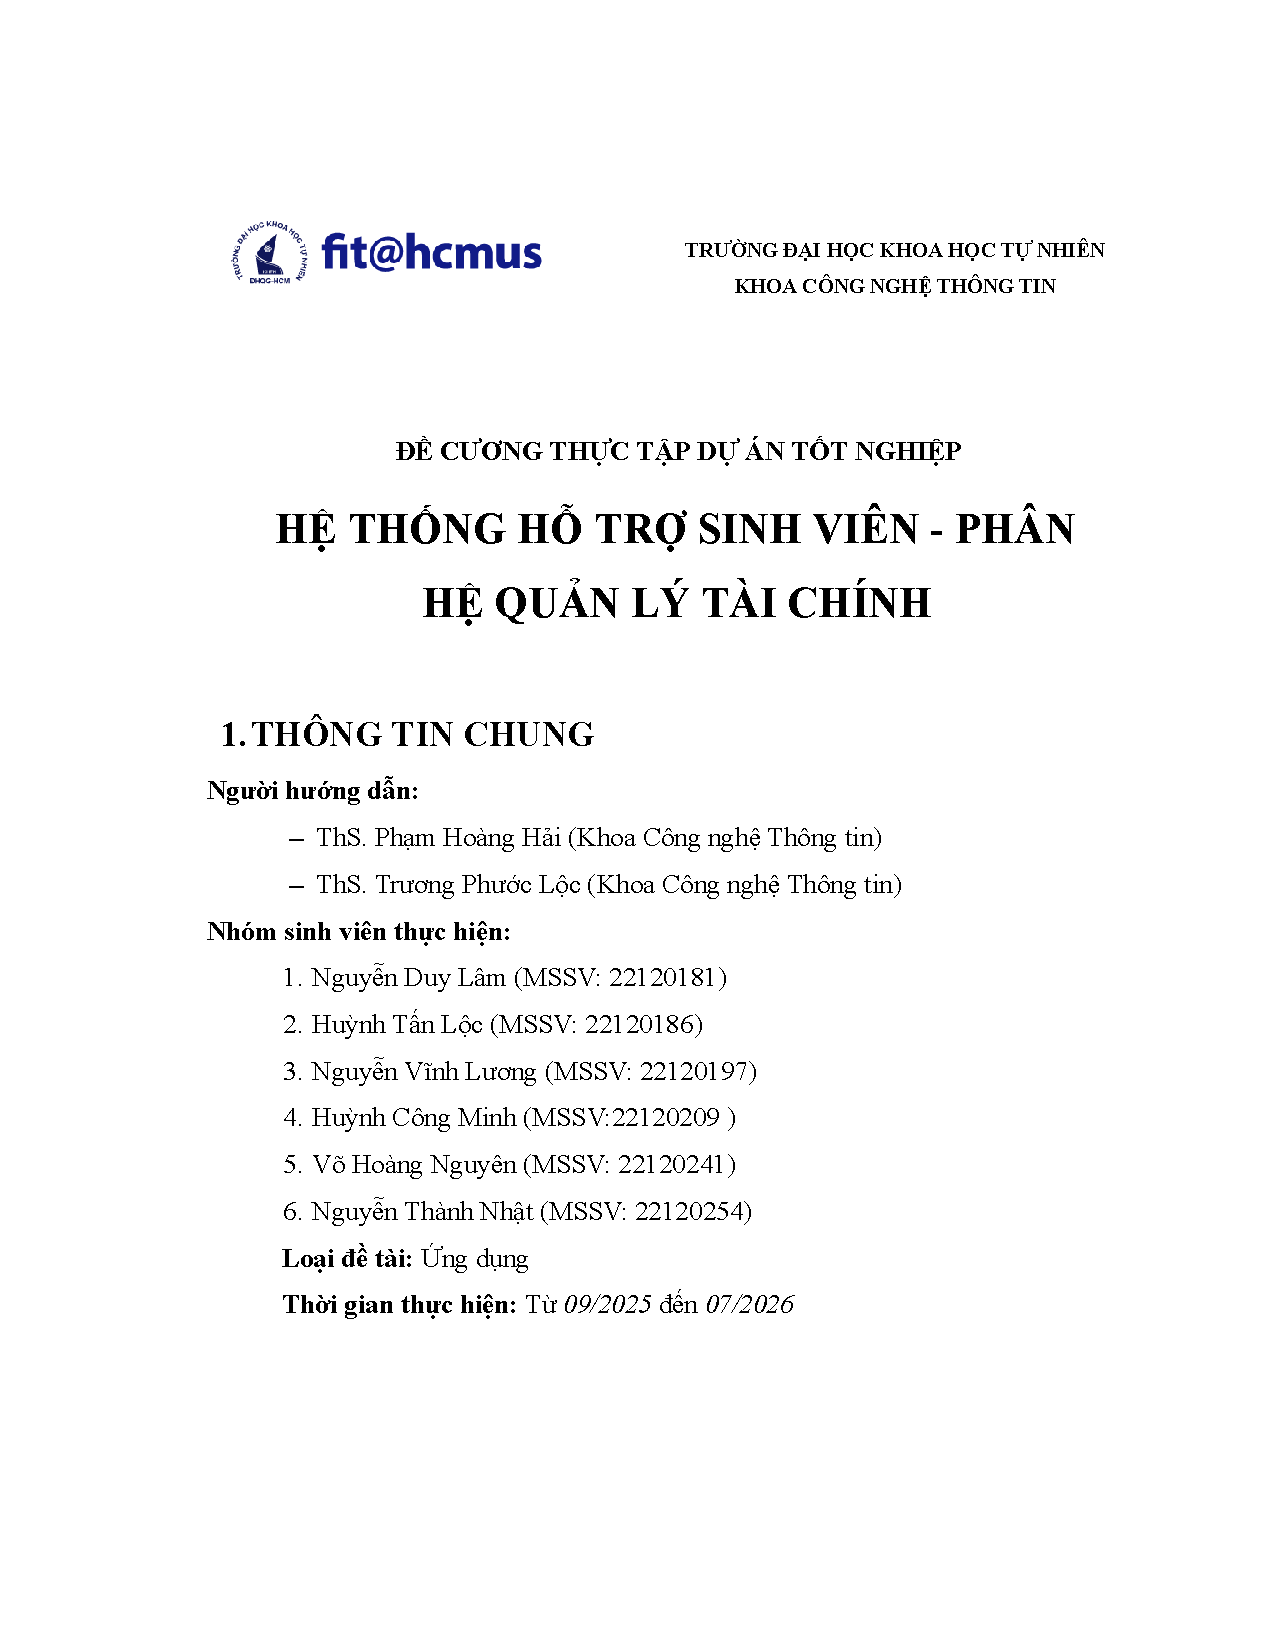
\includepdf[pages=-,pagecommand={\thispagestyle{empty}}]{[25D2-DA-KTPM10]_DeCuong_16032026.pdf}


% Mục lục, danh sách hình, danh sách bảng
\addcontentsline{toc}{chapter}{Mục lục}

\tableofcontents

%\listoffigures
\cleardoublepage
% \phantomsection
\addcontentsline{toc}{chapter}{\listfigurename}
\listoffigures

\cleardoublepage
% \phantomsection
\addcontentsline{toc}{chapter}{\listtablename}
\listoftables
%\listoftables

% Danh mục từ viết tắt (bắt buộc theo hướng dẫn KLTN)
\cleardoublepage
\addcontentsline{toc}{chapter}{Danh mục từ viết tắt}
\chapter*{Danh mục từ viết tắt}
\begin{longtable}{|l|l|p{8.5cm}|}
\hline
\textbf{STT} & \textbf{Từ viết tắt} & \textbf{Giải thích} \\
\hline
\endhead
1  & AI     & Trí tuệ nhân tạo (Artificial Intelligence) \\ \hline
2  & API    & Giao diện lập trình ứng dụng (Application Programming Interface) \\ \hline
3  & CCCD   & Căn cước công dân \\ \hline
4  & CRUD   & Tạo - Đọc - Cập nhật - Xóa (Create, Read, Update, Delete) \\ \hline
5  & DB     & Cơ sở dữ liệu (Database) \\ \hline
6  & DTO    & Đối tượng truyền dữ liệu (Data Transfer Object) \\ \hline
7  & ERD    & Sơ đồ thực thể liên kết (Entity Relationship Diagram) \\ \hline
8  & FCM    & Dịch vụ thông báo đám mây của Firebase (Firebase Cloud Messaging) \\ \hline
9  & GPA    & Điểm trung bình tích lũy (Grade Point Average) \\ \hline
10 & HTTP   & Giao thức truyền siêu văn bản (HyperText Transfer Protocol) \\ \hline
11 & JSON   & Ký hiệu đối tượng JavaScript (JavaScript Object Notation) \\ \hline
12 & JWT    & Mã thông báo JSON Web (JSON Web Token) \\ \hline
13 & LLM    & Mô hình ngôn ngữ lớn (Large Language Model) \\ \hline
14 & NLP    & Xử lý ngôn ngữ tự nhiên (Natural Language Processing) \\ \hline
15 & OCR    & Nhận dạng ký tự quang học (Optical Character Recognition) \\ \hline
16 & RBAC   & Kiểm soát truy cập dựa trên vai trò (Role-Based Access Control) \\ \hline
17 & REST   & Chuyển trạng thái đại diện (Representational State Transfer) \\ \hline
18 & SDK    & Bộ công cụ phát triển phần mềm (Software Development Kit) \\ \hline
19 & SSE    & Sự kiện gửi từ máy chủ (Server-Sent Events) \\ \hline
20 & TTL    & Thời gian sống của bộ nhớ đệm (Time-To-Live) \\ \hline
21 & UI     & Giao diện người dùng (User Interface) \\ \hline
22 & URL    & Định vị tài nguyên thống nhất (Uniform Resource Locator) \\ \hline
23 & UUID   & Định danh duy nhất toàn cầu (Universally Unique Identifier) \\ \hline
24 & UX     & Trải nghiệm người dùng (User Experience) \\ \hline
\end{longtable}

\addcontentsline{toc}{chapter}{Tóm tắt}
\chapter*{Tóm tắt}
\label{summary}

Trong đời sống giảng đường, sinh viên thường gặp khó khăn trong việc quản lý tài chính cá nhân một cách khoa học cũng như tiếp cận các thông tin học bổng phù hợp để hỗ trợ quá trình học tập. Nhằm giải quyết bài toán này, đề tài tập trung xây dựng và phát triển hệ thống hỗ trợ sinh viên toàn diện tích hợp Trí tuệ nhân tạo (AI) giúp quản lý tài chính cá nhân và tra cứu học bổng thông minh.

Hệ thống được thiết kế theo kiến trúc đa nền tảng bao gồm ứng dụng di động dành cho sinh viên và trang quản trị Web Admin dành cho người quản lý. Phân hệ tài chính cá nhân áp dụng phương pháp quản lý 6 chiếc lọ, kết hợp cùng trợ lý ảo AI để tư vấn chi tiêu và hỗ trợ lập kế hoạch tài chính hiệu quả. Bên cạnh đó, phân hệ học bổng tích hợp trợ lý AI giúp người dùng tìm kiếm, phân tích và gợi ý học bổng cá nhân hóa dựa trên hồ sơ sinh viên. Trang quản trị Web Admin được xây dựng đồng bộ nhằm phục vụ công tác quản lý thông tin học bổng, quản lý cơ cấu tổ chức trường và các khoa.

Kết quả thử nghiệm cho thấy hệ thống vận hành ổn định, giao diện trực quan, các mô hình AI phản hồi chính xác các truy vấn của người dùng với thời gian trễ thấp. Đề tài đóng góp một giải pháp công nghệ thiết thực, hỗ trợ sinh viên rèn luyện tư duy quản lý tài chính bền vững và gia tăng cơ hội tiếp cận học bổng, đồng thời cung cấp công cụ quản trị dữ liệu học tập hiệu quả cho các đơn vị quản lý.


\clearpage

\pagenumbering{arabic} % Đánh số 1, 2, 3, ...

% Các chương nội dung
\chapter{Giới thiệu}
\label{ch:gioi-thieu}

\section{Lý do chọn đề tài và bối cảnh nghiên cứu}
Trong kỷ nguyên số hóa hiện nay, đời sống sinh viên tại các trường Đại học đang đối mặt với nhiều biến động và thách thức to lớn. Sự chuyển dịch kinh tế kéo theo chi phí sinh hoạt, học phí và các nhu cầu dịch vụ học tập ngày càng gia tăng. Đối với phần lớn sinh viên, việc tự chủ cuộc sống khi bước vào môi trường đại học là một bước ngoặt lớn, đi kèm với áp lực tự quản lý bản thân trên nhiều phương diện. Trong số đó, hai vấn đề nổi cộm nhất ảnh hưởng trực tiếp đến chất lượng học tập và sự phát triển bền vững của sinh viên là quản lý tài chính cá nhân và cơ hội tiếp cận các nguồn lực hỗ trợ như học bổng học thuật.

Về khía cạnh quản lý tài chính cá nhân, sinh viên thường thiếu kiến thức nền tảng và kỹ năng quản lý dòng tiền. Thói quen chi tiêu tự phát, thiếu kế hoạch, và không kiểm soát được các khoản phát sinh dẫn đến tình trạng mất cân đối tài chính thường xuyên. Điều này không chỉ gây căng thẳng tâm lý mà còn gián tiếp làm suy giảm kết quả học tập khi sinh viên phải dành nhiều thời gian để đi làm thêm trang trải cuộc sống. Phương pháp quản lý tài chính "6 cái lọ" (6 Jars) của T. Harv Eker là một mô hình nổi tiếng thế giới, giúp phân bổ thu nhập một cách khoa học vào các quỹ chi tiêu thiết yếu, đầu tư, giáo dục, tiết kiệm dài hạn, hưởng thụ và từ thiện \cite{eker2005-6jars}. Tuy nhiên, việc áp dụng mô hình này một cách thủ công thường gặp nhiều khó khăn do tính phức tạp trong việc ghi chép, phân loại giao dịch hàng ngày và thiếu tính kỷ luật tự giác.

Về khía cạnh tiếp cận nguồn lực hỗ trợ, học bổng là một trong những mục tiêu quan trọng giúp sinh viên giảm bớt gánh nặng tài chính và tạo động lực phấn đấu trong học tập. Hiện nay, các nguồn thông tin về học bổng rất đa dạng nhưng phân tán từ nhiều nhà tài trợ, doanh nghiệp, tổ chức phi chính phủ đến chính sách nội bộ của từng trường. Sinh viên thường bỏ lỡ các cơ hội học bổng phù hợp do không tiếp cận được thông tin kịp thời hoặc hồ sơ năng lực cá nhân chưa được so khớp tối ưu với các tiêu chí xét tuyển phức tạp. Đồng thời, các nhà tài trợ cũng gặp khó khăn trong việc tìm kiếm đúng đối tượng sinh viên đáp ứng đầy đủ yêu cầu học thuật và hoàn cảnh cụ thể.

Xuất phát từ thực trạng trên, đề tài \textbf{"Hệ thống hỗ trợ sinh viên - phân hệ quản lý tài chính"} được nghiên cứu và phát triển. Đề tài hướng tới việc xây dựng một hệ sinh thái tích hợp đa nền tảng, áp dụng các giải pháp công nghệ hiện đại và trí tuệ nhân tạo (AI) để giải quyết triệt để hai bài toán cốt lõi: tự động hóa quản lý tài chính cá nhân theo mô hình 6 lọ và tối ưu hóa quy trình so khớp học bổng thông minh cho sinh viên.

\section{Mục tiêu và phạm vi nghiên cứu}
\subsection{Mục tiêu nghiên cứu}
Đề tài tập trung vào việc nghiên cứu, thiết kế và phát triển các mục tiêu cụ thể sau:
\begin{itemize}
    \item Nghiên cứu cơ sở lý thuyết và hiện thực hóa mô hình quản lý tài chính cá nhân "6 chiếc lọ" trên ứng dụng di động, giúp sinh viên thiết lập và duy trì thói quen chi tiêu khoa học.
    \item Ứng dụng trí tuệ nhân tạo (AI Agent và Large Language Models - LLM) để tự động hóa quy trình phân loại giao dịch tài chính từ ngôn ngữ tự nhiên, cũng như tư vấn tài chính cá nhân thời gian thực thông qua Chatbot trợ lý ảo.
    \item Xây dựng phân hệ học bổng trực tuyến cho phép nhà tài trợ tạo chương trình học bổng, cấu hình điều kiện và tài liệu yêu cầu; đồng thời hỗ trợ sinh viên lưu nháp, nộp, theo dõi và hủy hồ sơ ứng tuyển theo quy trình xử lý rõ ràng.
    \item Xây dựng hệ thống đẩy thông báo di động (FCM Push Notification) thông minh, chạy ngầm định kỳ nhằm đưa ra các cảnh báo tài chính chủ động và thông tin học bổng khẩn cấp tới sinh viên.
    \item Xây dựng phân hệ quản trị dữ liệu học thuật cho phép quản trị viên quản lý danh mục trường đại học, khoa/chương trình đào tạo và môn học; đồng thời hỗ trợ sinh viên lập bảng điểm cá nhân, theo dõi GPA, tổng tín chỉ và mục tiêu học tập.
\end{itemize}

\subsection{Phạm vi nghiên cứu}
\begin{itemize}
    \item \textbf{Về đối tượng nghiên cứu:} Tập trung vào hành vi tài chính, chi tiêu sinh hoạt thường nhật và hồ sơ năng lực học thuật của sinh viên đại học.
    \item \textbf{Về mặt công nghệ:} Phát triển hệ thống đa dịch vụ (Monorepo) tích hợp: Backend (NestJS, TypeScript), AI Service (FastAPI, Python, LangChain, Google Vertex API), Mobile App (Expo React Native), và Web Portal Admin (React JS, Material UI).
    \item \textbf{Về mặt dữ liệu:} Khai thác dữ liệu học thuật mẫu mô phỏng theo cấu trúc đào tạo tín chỉ tại các trường đại học lớn tại Việt Nam (điển hình là mô hình Đại học Quốc gia TP.HCM).
\end{itemize}

\section{Mô tả bài toán đề tài giải quyết}
\subsection{Bài toán quản lý tài chính cá nhân sinh viên theo phương pháp 6 lọ}
Bài toán yêu cầu xây dựng một mô hình số hóa 6 quỹ tài chính độc lập cho từng người dùng, đảm bảo các nguyên tắc:
\begin{itemize}
    \item \textbf{Tính phân bổ tự động:} Khi người dùng phát sinh nguồn thu nhập mới (lương, học bổng, trợ cấp), hệ thống phải tự động phân chia dòng tiền vào 6 lọ theo tỷ lệ phần trăm được cấu hình trước.
    \item \textbf{Tính toàn vẹn dữ liệu tài chính:} Số dư của từng hũ tài chính phải là kết quả tính toán động từ dòng tiền thu chi thực tế trong lịch sử giao dịch để tránh sai lệch số liệu. Khi có hành vi xóa hoặc rebalance (điều chỉnh tỷ lệ hũ), hệ thống phải thực hiện các giao dịch bù trừ nội bộ để đảm bảo tổng tài sản của người dùng không bị thay đổi bất thường.
    \item \textbf{Hạn mức ngân sách (Budgeting):} Cho phép người dùng giới hạn chi tiêu trong từng lọ theo chu kỳ tháng để cảnh báo khi chi tiêu vượt ngưỡng thiết yếu.
\end{itemize}

\subsection{Bài toán quản lý và ứng tuyển học bổng trực tuyến}
Bài toán đặt ra là làm thế nào để số hóa toàn bộ quy trình công bố, tiếp nhận và xét duyệt học bổng giữa nhà tài trợ và sinh viên. Mỗi chương trình học bổng có thông tin riêng về giá trị tài trợ, số lượng suất, thời hạn nộp, điều kiện GPA, ngành học, trường mục tiêu và bộ tài liệu yêu cầu. Hệ thống cần đảm bảo sinh viên có thể tiếp cận thông tin rõ ràng, chuẩn bị hồ sơ trực tuyến và theo dõi trạng thái xử lý sau khi nộp.

Đối với nhà tài trợ, hệ thống cần cung cấp cổng quản trị để tạo và cập nhật học bổng, cấu hình điều kiện xét tuyển, định nghĩa các tài liệu bắt buộc và xem danh sách hồ sơ ứng tuyển theo từng chương trình. Đối với sinh viên, hệ thống cần hỗ trợ lưu nháp, nộp hồ sơ, upload tài liệu minh chứng, cập nhật hồ sơ khi được yêu cầu bổ sung và hủy hồ sơ khi còn trong trạng thái cho phép.

\subsection{Bài toán quản trị cơ sở dữ liệu học thuật của trường học}
Để dữ liệu học thuật được sử dụng thống nhất giữa Webadmin và ứng dụng di động, hệ thống cần số hóa quy trình quản lý danh mục trường đại học, khoa/chương trình đào tạo và môn học. Mỗi trường có thể có nhiều chương trình đào tạo và nhiều môn học. Mỗi môn học cần lưu mã môn, tên môn, mã học phần, số tín chỉ, thang điểm và trạng thái hoạt động để phục vụ quá trình nhập điểm của sinh viên.

Đối với quản trị viên, hệ thống cần cung cấp giao diện tạo, cập nhật, xóa, tìm kiếm và import hàng loạt dữ liệu trường, khoa/chương trình đào tạo và môn học. Đối với sinh viên, hệ thống cần cho phép chọn trường và chương trình đào tạo từ danh mục có sẵn, sau đó sử dụng danh mục môn học của trường để nhập điểm, import bảng điểm, theo dõi GPA và tiến độ tín chỉ.

\subsection{Các câu hỏi nghiên cứu}
Để định hướng triển khai và đánh giá hiệu quả các giải pháp kỹ thuật đề xuất, đề tài tập trung trả lời hai câu hỏi nghiên cứu cốt lõi sau:
\begin{enumerate}
    \item \textbf{CH1 -- Phân loại giao dịch:} Làm thế nào để tự động hóa việc phân loại các giao dịch tài chính từ ngôn ngữ tự nhiên phi chuẩn (viết tắt, sai chính tả tiếng Việt) của sinh viên vào đúng hũ tài chính trong mô hình 6 lọ với độ chính xác cao mà không làm chậm trải nghiệm người dùng?
    \item \textbf{CH2 -- Quản lý học bổng:} Làm thế nào để thiết kế quy trình học bổng trực tuyến đảm bảo nhà tài trợ có thể công bố chương trình, sinh viên nộp hồ sơ hợp lệ, và hệ thống theo dõi được toàn bộ trạng thái xét duyệt từ lưu nháp, đã nộp, đang xét duyệt đến phê duyệt hoặc từ chối?
    \item \textbf{CH3 -- Hệ thống thông báo hiệu năng cao:} Kiến trúc hàng đợi tin nhắn cần được thiết kế như thế nào để đảm bảo tính sẵn sàng cao và không gây nghẽn hệ thống khi gửi đồng loạt hàng nghìn thông báo đẩy di động (FCM) tới các sinh viên cùng lúc?
\end{enumerate}

\section{Những thách thức và hướng giải quyết của đề tài}
\subsection{Những thách thức lớn}
Trong quá trình xây dựng hệ thống, nhóm nghiên cứu đối mặt với các thách thức chính sau:
\begin{enumerate}
    \item \textbf{Độ trễ và chi phí tích hợp AI:} Việc gọi trực tiếp các API của mô hình ngôn ngữ lớn (như Gemini) có độ trễ phản hồi tương đối cao và tốn kém tài nguyên.
    \item \textbf{Tính chính xác trong phân loại giao dịch:} Ngôn ngữ tự nhiên mà người dùng nhập vào khi ghi chép chi tiêu thường mang tính viết tắt, không chuẩn hóa ngữ pháp (ví dụ: "an trua 50k", "cf 30k").
    \item \textbf{Đồng bộ trạng thái giao diện thời gian thực:} Giao diện điện thoại di động yêu cầu cập nhật tức thì số dư của các hũ và biểu đồ báo cáo ngay sau khi người dùng thực hiện giao dịch mà không làm chậm trải nghiệm ứng dụng.
    \item \textbf{Bảo mật dữ liệu và phân quyền hệ thống:} Dữ liệu tài chính cá nhân và hồ sơ học thuật/học bổng của sinh viên là các thông tin nhạy cảm. Hệ thống cần đảm bảo an toàn truy cập dữ liệu, chỉ cho phép các đối tượng thích hợp tiếp cận các tập tài nguyên tương ứng (Sinh viên truy cập app cá nhân, Nhà tài trợ quản lý hồ sơ ứng tuyển, Admin quản trị hệ thống).
    \item \textbf{Đảm bảo tính nhất quán và toàn vẹn của dữ liệu giao dịch tài chính:} Khi thực hiện các tác vụ phức tạp như phân bổ thu nhập (income distribution) vào 6 hũ hoặc cập nhật thông tin hũ, việc phát sinh lỗi giữa chừng hoặc race conditions có thể dẫn đến sai lệch số dư.
    \item \textbf{Đồng bộ dữ liệu học thuật và bảng điểm cá nhân:} Danh mục trường, khoa/chương trình đào tạo và môn học cần nhất quán giữa Webadmin và Mobile App. Đồng thời, điểm sinh viên nhập phải được kiểm tra theo thang điểm của từng môn, tránh sai lệch GPA và tổng tín chỉ.
\end{enumerate}

\subsection{Hướng tiếp cận giải quyết}
Để vượt qua các thách thức trên, đề tài đề xuất các hướng giải quyết kỹ thuật cụ thể:
\begin{itemize}
    \item \textbf{Sử dụng kiến trúc AI Agent và Caching:} FastAPI AI Service được thiết kế độc lập, đóng vai trò điều phối (orchestration) sử dụng các Tool-calling Agent của LangChain để tối ưu hóa việc gọi mô hình. Áp dụng cơ chế lưu đệm Redis Caching với TTL (Time-to-Live) từ 5-15 phút tại Backend để lưu trữ các nhận định tài chính (AI Insights), giảm tải số lượng request trùng lặp gửi đến Gemini API.
    \item \textbf{Huấn luyện LLM Classifier với Rule Engine:} Sử dụng các bộ quy tắc gán cứng (Rule-based) kết hợp với kỹ thuật Few-shot Prompting để hướng dẫn mô hình Gemini phân loại các thuật ngữ viết tắt của người dùng một cách chính xác vào 6 lọ tài chính.
    \item \textbf{Đồng bộ giao diện qua React Query:} Áp dụng thư viện quản lý state React Query (TanStack Query) trên Expo Frontend để quản lý cơ chế Invalidation. Khi có bất kỳ thay đổi nào từ phía dữ liệu, hệ thống tự động làm mới bộ đệm cục bộ và render lại màn hình mà không cần reload toàn bộ app.
    \item \textbf{Xác thực JWT và cơ chế phân quyền RolesGuard:} Sử dụng JSON Web Token (JWT) để xác thực người dùng trên các API. Triển khai bộ phân quyền `RolesGuard` chặt chẽ trong NestJS để phân tách quyền truy cập dựa trên vai trò (Student, Donor, Admin), bảo vệ an toàn cho các endpoint nhạy cảm.
    \item \textbf{Quản lý dữ liệu qua Database Transactions và cơ chế recalculate số dư:} Áp dụng cơ chế transaction của TypeORM trong NestJS để đảm bảo tính nguyên tử (Atomicity) cho các tác vụ cập nhật tài chính và hồ sơ học bổng. Đồng thời, xây dựng hàm tính toán lại số dư (`recalculateJarBalance`) dựa trên lịch sử giao dịch thực tế để chống sai lệch.
    \item \textbf{Thiết kế cơ sở dữ liệu quan hệ chuẩn hóa cao trên PostgreSQL:} Xây dựng cấu trúc cơ sở dữ liệu với các ràng buộc khóa ngoại (Foreign Keys) chặt chẽ tại Webadmin để đồng bộ dữ liệu học thuật phân cấp từ trường học tới sinh viên, đảm bảo tính nhất quán toàn vẹn dữ liệu.
\end{itemize}

\section{Các đóng góp của đề tài}
Đề tài mang lại các đóng góp thiết thực cả về mặt học thuật lẫn ứng dụng thực tiễn:
\begin{itemize}
    \item \textbf{Về mặt công nghệ:} Hiện thực hóa thành công một kiến trúc Monorepo đa dịch vụ ổn định, giải quyết bài toán giao tiếp bất đồng bộ và đồng bộ trạng thái giao diện thời gian thực giữa thiết bị di động, máy chủ API và lõi AI.
    \item \textbf{Về mặt ứng dụng tài chính:} Số hóa thành công mô hình quản lý tài chính 6 lọ, bổ sung thêm các tính năng thông minh như cảnh báo ngân sách tự động, gợi ý tái cấu trúc hũ hằng tháng (Jars Rebalancing) và trợ lý ảo tư vấn tài chính thân thiện với sinh viên.
    \item \textbf{Về hỗ trợ học tập:} Xây dựng phân hệ quản lý dữ liệu học thuật và bảng điểm cá nhân, giúp sinh viên theo dõi GPA, tín chỉ tích lũy, mục tiêu tín chỉ và quản lý điểm theo danh mục môn học chuẩn hóa từ nhà trường.
\end{itemize}


\chapter{Khảo sát và phân tích các giải pháp liên quan}
\label{ch:cong-trinh-lien-quan}

\section{Các hệ thống quản lý tài chính cá nhân hiện có và hạn chế}
Trong quá trình xây dựng giải pháp, nhóm tiến hành khảo sát các ứng dụng phổ biến trên thị trường, tiêu biểu như Money Lover, Spendee và Wallet by BudgetBakers:
\begin{itemize}
    \item \textbf{Money Lover (v4.0.x):} Ứng dụng nổi tiếng tại Việt Nam do ZooStudio phát triển. Hỗ trợ ghi chép chi tiêu, lập ngân sách định kỳ, quét hóa đơn qua ảnh và biểu đồ thống kê trực quan. Liên kết tài khoản ngân hàng chỉ có ở gói Premium.
    \item \textbf{Spendee (v5.1.x):} Giao diện hiện đại, tập trung vào ví dùng chung (Shared Wallets) cho gia đình hoặc nhóm bạn. Hầu hết tính năng nâng cao yêu cầu tài khoản trả phí.
    \item \textbf{Wallet by BudgetBakers (v8.4.x):} Cung cấp báo cáo tài chính chuyên sâu, hỗ trợ nhiều loại tiền tệ và đồng bộ hóa tự động với hơn 4.000 ngân hàng đối tác.
\end{itemize}

\begin{figure}[H]
    \centering
    \begin{minipage}{0.45\textwidth}
        \centering
        
\includegraphics[height=8.5cm]{chapter2/money_lover_1.jpg}
        \centerline{(a) Giao diện ghi chép chi tiêu}
    \end{minipage}
    \hfill
    \begin{minipage}{0.45\textwidth}
        \centering
        
\includegraphics[height=8.5cm]{chapter2/money_lover_2.jpg}
        \centerline{(b) Biểu đồ phân tích thu chi}
    \end{minipage}
    \caption{Giao diện khảo sát ứng dụng Money Lover}
    \label{fig:survey-money-lover}
\end{figure}

\begin{figure}[H]
    \centering
    \begin{minipage}{0.45\textwidth}
        \centering
        
\includegraphics[height=8.5cm]{chapter2/spendee_1.jpg}
        \centerline{(a) Thiết lập hạn mức ngân sách}
    \end{minipage}
    \hfill
    \begin{minipage}{0.45\textwidth}
        \centering
        
\includegraphics[height=8.5cm]{chapter2/spendee_2.jpg}
        \centerline{(b) Quản lý ví nhóm dùng chung}
    \end{minipage}
    \caption{Giao diện khảo sát ứng dụng Spendee}
    \label{fig:survey-spendee}
\end{figure}

\begin{figure}[H]
    \centering
    \begin{minipage}{0.31\textwidth}
        \centering
        
\includegraphics[height=8.5cm]{chapter2/wallet_1.jpg}
        \centerline{(a) Tổng quan tài khoản}
    \end{minipage}
    \hfill
    \begin{minipage}{0.31\textwidth}
        \centering
        
\includegraphics[height=8.5cm]{chapter2/wallet_2.jpg}
        \centerline{(b) Liên kết ngân hàng}
    \end{minipage}
    \hfill
    \begin{minipage}{0.31\textwidth}
        \centering
        
\includegraphics[height=8.5cm]{chapter2/wallet_3.jpg}
        \centerline{(c) Biểu đồ báo cáo}
    \end{minipage}
    \caption{Giao diện khảo sát ứng dụng Wallet by BudgetBakers}
    \label{fig:survey-wallet}
\end{figure}
\subsection{Phương pháp và nghị trình khảo sát các giải pháp thị trường}
Nhóm thiết lập một quy trình khảo sát hệ thống (Survey Protocol) với các tiêu chí cụ thể:
\begin{itemize}
    \item \textbf{Phạm vi thời gian:} Khảo sát tiến hành từ tháng 09/2025 đến 02/2026. Ngày truy cập kiểm tra cuối cùng là 15/02/2026.
    \item \textbf{Từ khóa tìm kiếm:} Sử dụng từ khóa tiếng Anh và tiếng Việt trên Google Play, App Store và công cụ tìm kiếm: ``personal finance manager'', ``scholarship finder'', ``GPA calculator'', ``quản lý tài chính cá nhân'', ``học bổng sinh viên''.
    \item \textbf{Tiêu chí lựa chọn (Inclusion):}
    \begin{itemize}
        \item Phân hệ tài chính: Ứng dụng di động trên 100.000 lượt tải, hỗ trợ tiếng Anh hoặc tiếng Việt, tương thích thị trường Việt Nam.
        \item Phân hệ học bổng và học thuật: Cổng thông tin có lượng người dùng hoạt động thường xuyên hoặc là kênh chính thức của các cơ sở đại học lớn.
    \end{itemize}
    \item \textbf{Tiêu chí loại trừ (Exclusion):} Ứng dụng ngừng cập nhật trước năm 2024, giải pháp đóng phí bắt buộc 100\% ngay khi cài đặt, hoặc bảng tính Excel cá nhân không phân phối rộng rãi.
\end{itemize}

Để tổng hợp sự đối lập giữa các giải pháp hiện tại với Student360, nhóm xây dựng bảng ma trận so sánh tính năng cốt lõi trong Bảng~\ref{tab:so-sanh-giai-phap}.

\begin{table}[H]
\centering
\begin{tabular}{|L{3.2cm}|C{2.0cm}|C{2.0cm}|C{2.0cm}|L{2.5cm}|L{2.6cm}|}
\hline
\textbf{Tiêu chí đối sánh} & \textbf{Money Lover} & \textbf{Spendee} & \textbf{Wallet} & \textbf{Các giải pháp truyền thống} & \textbf{Đề tài Student360} \\ \hline
Ghi chép giao dịch & Có (Miễn phí / Trả phí) & Có (Miễn phí / Trả phí) & Có (Miễn phí / Trả phí) & Không hỗ trợ & Có (Miễn phí hoàn toàn) \\ \hline
Tự động hóa chia 6 lọ tài chính & Một phần (phải cấu hình ví thủ công) & Không hỗ trợ & Không hỗ trợ & Không hỗ trợ & Có (Hỗ trợ cấu hình và chia tự động) \\ \hline
Phân loại bằng AI & Thô sơ (Regex / Khớp chuỗi) & Không hỗ trợ & Không hỗ trợ & Không hỗ trợ & Có (LLM Few-shot + Rules) \\ \hline
Cảnh báo ngân sách chủ động & Có (Hạn mức tĩnh theo tháng) & Có (Hạn mức theo ví) & Có (Thống kê tĩnh) & Không hỗ trợ & Có (Đa lớp, thời gian thực qua FCM) \\ \hline
Liên kết học bổng & Không hỗ trợ & Không hỗ trợ & Không hỗ trợ & Lọc cứng thủ công qua tin bài & Có (So khớp hồ sơ tự động) \\ \hline
Quản lý học thuật & Không hỗ trợ & Không hỗ trợ & Không hỗ trợ & Tách biệt trên cổng Student Portal & Có (Tính toán GPA và tiến độ tích lũy) \\ \hline
Tương tác AI Agent & Không hỗ trợ & Không hỗ trợ & Không hỗ trợ & Không hỗ trợ & Có (Trò chuyện thời gian thực qua SSE) \\ \hline
\end{tabular}

\caption{Bảng ma trận đối sánh tính năng giữa các giải pháp thị trường và đề tài Student360}
\label{tab:so-sanh-giai-phap}
\end{table}

\subsection{Hạn chế đối với đối tượng sinh viên}
Các ứng dụng trên đã giải quyết được nhiều nhu cầu cơ bản, nhưng vẫn tồn tại các hạn chế cốt lõi đối với sinh viên:
\begin{enumerate}
    \item \textbf{Thiếu tích hợp sâu mô hình 6 lọ:} Người dùng phải tự tính toán tỷ lệ phân bổ và chia nhỏ dòng tiền thủ công mỗi khi có thu nhập mới. Chưa ứng dụng nào số hóa quy chuẩn mô hình ``6 cái lọ'' của T. Harv Eker \cite{eker2005-6jars}.
    \item \textbf{Mức độ tự động hóa bằng AI còn thấp:} Đa số chỉ dùng thuật toán so khớp chuỗi (string matching) hoặc biểu thức chính quy để phân loại giao dịch. Khi người dùng nhập mô tả viết tắt hoặc sai chính tả, hệ thống không nhận diện được và buộc chọn danh mục thủ công.
    \item \textbf{Thiếu tính chủ động và cá nhân hóa (Proactivity):} Các ứng dụng hoạt động theo mô hình thụ động -- chỉ ghi nhận và thống kê sau khi giao dịch xảy ra. Hệ thống thiếu cơ chế phân tích hành vi ngầm để cảnh báo chi tiêu vượt hạn mức hoặc gợi ý tái cấu trúc dòng tiền trước khi sự cố xảy ra.
\end{enumerate}

\section{Các giải pháp kết nối học bổng truyền thống}
Đối với sinh viên Việt Nam, thông tin học bổng thường được công bố qua các kênh truyền thống:
\begin{itemize}
    \item Trang web chính thức của Phòng Công tác Sinh viên (CTSV) hoặc Giáo vụ khoa của các trường Đại học.
    \item Các diễn đàn trực tuyến, mạng xã hội (Facebook, LinkedIn).
    \item Các trang tin học bổng chuyên biệt (ví dụ: Scholarship Planet, YBOX).
\end{itemize}

Các phương thức này bộc lộ nhiều hạn chế:
\begin{enumerate}
    \item \textbf{Thông tin bị phân mảnh và chậm trễ:} Sinh viên phải truy cập thủ công nhiều trang web. Nhiều học bổng có thời gian ứng tuyển ngắn, sinh viên thường chỉ phát hiện khi sát hạn nộp.
    \item \textbf{Cơ chế lọc thô sơ:} Các trang tin chỉ hỗ trợ lọc theo tiêu chí cứng cơ bản (Quốc gia, Ngành học chung). Sinh viên không biết hồ sơ của mình đáp ứng bao nhiêu phần trăm điều kiện của học bổng.
    \item \textbf{Gánh nặng cho nhà tài trợ và ban quản trị:} Quy trình xét duyệt hồ sơ đa phần vẫn thực hiện thủ công qua email hoặc Google Forms, gây khó khăn quản lý tập trung và dễ xảy ra sai sót.
\end{enumerate}

\section{Các giải pháp quản lý học thuật và bảng điểm hiện có}
Các giải pháp hiện có cho nhu cầu theo dõi kết quả học tập thuộc một trong hai nhóm:
\begin{itemize}
    \item \textbf{Cổng thông tin sinh viên (Student Portal):} Kênh chính thức để tra cứu điểm số sau khi nhà trường công bố. Đảm bảo tính chính xác nhưng không hỗ trợ sinh viên tự nhập điểm dự kiến để mô phỏng kịch bản GPA, và hoàn toàn tách biệt với nhu cầu tài chính hay học bổng.
    \item \textbf{Ứng dụng tính GPA độc lập:} Cho phép nhập điểm và số tín chỉ để tính GPA tích lũy. Tuy nhiên không đồng bộ với danh mục môn học chuẩn hóa của từng trường, dễ dẫn đến sai lệch khi trường có môn trùng tên nhưng khác số tín chỉ.
\end{itemize}

Cả hai nhóm đều tồn tại hạn chế chung:
\begin{enumerate}
    \item \textbf{Thiếu liên kết giữa dữ liệu học thuật và các nhu cầu khác:} GPA là tiêu chí xét duyệt quan trọng của nhiều học bổng, nhưng sinh viên phải tự tổng hợp thủ công từ cổng trường để điền vào hồ sơ ứng tuyển ở hệ thống khác -- không có cơ chế đối chiếu tự động.
    \item \textbf{Không chuẩn hóa dữ liệu môn học giữa các trường:} Do mỗi trường có mã môn, số tín chỉ và thang điểm riêng, các ứng dụng tính GPA độc lập không thể tự động xác thực dữ liệu, dẫn đến sai số tích lũy.
\end{enumerate}

\section{Nghiên cứu liên quan và ứng dụng trí tuệ nhân tạo}
\label{sec:nghien-cuu-lien-quan}
Sự bùng nổ của Mô hình ngôn ngữ lớn (LLM) và hệ thống đại lý thông minh (AI Agents) đã mở ra hướng giải quyết mới cho bài toán quản lý và gợi ý thông tin trong giáo dục. Phần này tổng hợp các nghiên cứu liên quan gần đây theo nhóm phương pháp và kết quả.

\subsection{Lĩnh vực quản lý tài chính cá nhân (Personal Finance Management)}
\begin{itemize}
    \item \textbf{Phương pháp:} Nghiên cứu truyền thống áp dụng SVM, Naive Bayes hoặc cây quyết định để phân loại văn bản giao dịch. Xu hướng gần đây chuyển sang các mô hình Transformer \cite{vaswani2017attention} như BERT \cite{devlin2018bert} hoặc LLM thông qua kỹ thuật Few-shot Prompting \cite{brown2020-gpt3}.
    \item \textbf{Dữ liệu:} Chuỗi văn bản mô tả giao dịch ngắn (dưới 15 từ) từ người dùng di động, chứa nhiều từ viết tắt hoặc lỗi chính tả (ví dụ: ``mua banh mi 15k'', ``tna 50k'').
    \item \textbf{Kết quả:} LLM kết hợp Few-shot Prompting và Chain-of-Thought \cite{wei2022-cot} cải thiện F1-Score từ 15\% đến 25\% so với phương pháp cũ mà không cần fine-tuning lại mô hình.
\end{itemize}

\subsection{Lĩnh vực gợi ý học bổng (Scholarship Recommender Systems)}
\begin{itemize}
    \item \textbf{Phương pháp:} Hai hướng chính: Lọc dựa trên nội dung (Content-based filtering) dùng TF-IDF, Cosine hoặc Jaccard \cite{jaccard1901}, và Lọc cộng tác (Collaborative filtering). Do dữ liệu tương tác thưa thớt, các nghiên cứu hiện đại ưu tiên hệ gợi ý kết hợp (Hybrid Recommender Systems) \cite{burke2002hybrid, adomavicius2005toward} để khắc phục Cold Start.
    \item \textbf{Kết quả:} Kết hợp Fuzzy Matching cấp độ token (Jaccard) và ký tự (N-gram \cite{cavnar1994-ngram}, Levenshtein \cite{levenstein1966}) giúp hệ thống chịu lỗi viết tắt tốt hơn. Các hệ thống hybrid đạt Precision@5 trên 80\% trong môi trường thử nghiệm học thuật.
\end{itemize}

\subsection{Lĩnh vực Tác nhân AI hỗ trợ (LLM-based Agents)}
\begin{itemize}
    \item \textbf{Phương pháp:} Kiến trúc Tác nhân AI tự trị (Autonomous Agents) \cite{wang2023survey-agent} theo mô hình ReAct (Reasoning and Acting) \cite{yao2022-react}: LLM thực hiện vòng lặp suy luận ý định $\rightarrow$ gọi công cụ bên ngoài (truy vấn CSDL, gọi API) $\rightarrow$ nhận kết quả $\rightarrow$ tiếp tục suy luận hoặc đưa ra câu trả lời.
    \item \textbf{Kết quả:} ReAct kết hợp Tool-calling giúp AI Agent truy vấn số dư thực tế, đưa ra nhận định tài chính cá nhân hóa và định tuyến chính xác ý định tìm kiếm học bổng.
\end{itemize}

\section{Các giải pháp thông báo đẩy thời gian thực trên nền tảng di động}
Hệ thống thông báo đẩy (Push Notification) đóng vai trò quan trọng trong việc tăng tỷ lệ giữ chân người dùng. Các công nghệ được Student360 áp dụng:
\begin{itemize}
    \item \textbf{Firebase Cloud Messaging (FCM) \cite{fcm-docs}:} Dịch vụ đám mây của Google, gửi thông báo đến thiết bị Android và iOS kể cả khi ứng dụng đã bị đóng (Background/Killed state). FCM tối ưu hóa thời lượng pin bằng cách gom nhóm kết nối mạng ngầm. Đây là lựa chọn chính để gửi thông báo học bổng và cảnh báo tài chính.
    \item \textbf{BullMQ và Redis Queue \cite{bullmq-docs}:} Để xử lý gửi thông báo đến hàng nghìn thiết bị mà không làm nghẽn tiến trình chính, hệ thống áp dụng kiến trúc hàng đợi thông điệp. BullMQ kết hợp Redis \cite{redis-docs} quản lý thứ tự gửi, xử lý lỗi tự động và phân bổ tài nguyên tối ưu. Điểm khác biệt cốt lõi là kiến trúc thông báo \textbf{chủ động đa lớp} với nhiều loại thông báo Cron tự động:
    \begin{enumerate}
        \item \textbf{Cảnh báo ngưỡng số dư hũ} (theo số tiền tuyệt đối hoặc phần trăm ngân sách): kích hoạt ngay sau mỗi giao dịch chi tiêu theo kiểu fire-and-forget.
        \item \textbf{Cảnh báo ngân sách hũ sắp hết hoặc đã cạn}: gửi khi số dư còn lại $\leq 10\%$ hoặc đã âm.
        \item \textbf{Nhắc lịch chuyển tiền tự động sắp đến}: gửi 24 giờ trước ngày thực hiện, kèm xác nhận sau khi chuyển thành công hoặc thất bại.
        \item \textbf{Tóm tắt chi tiêu tuần} (Cron thứ Hai 8:00): tổng hợp tổng thu, tổng chi và hũ chi nhiều nhất trong tuần.
        \item \textbf{Báo cáo tài chính cuối tháng} (Cron ngày 1 hàng tháng 8:00): nhắc xem phân tích AI 6 lọ.
        \item \textbf{Nhắc nhở cập nhật tài chính} (Cron thứ Hai 9:00): gửi cho người dùng không nhập giao dịch nào trong 7 ngày gần nhất.
        \item \textbf{Nhắc lịch chuyển tiền sắp kết thúc} (Cron thứ Hai 9:00): gửi cho các lịch chuyển tiền sắp hết hạn trong vòng 3 ngày tới.
    \end{enumerate}
    Nhờ kiến trúc này, hệ thống chủ động tương tác với người dùng đúng ngữ cảnh, thay vì chỉ phản ứng khi người dùng mở ứng dụng.
\end{itemize}

\section{Rủi ro đạo đức và giải pháp đảm bảo trách nhiệm AI (Responsible AI)}
Trong hệ thống phần mềm tích hợp AI như Student360, việc xem xét rủi ro đạo đức và thực thi nguyên tắc Responsible AI là bắt buộc. Nhóm phân tích bốn khía cạnh rủi ro cốt lõi:

\begin{enumerate}
    \item \textbf{Thiên lệch trong gợi ý thuật toán (Algorithmic Bias):}
    \begin{itemize}
        \item \textit{Rủi ro:} Thuật toán có xu hướng ưu tiên sinh viên có hồ sơ học thuật xuất sắc, bỏ qua sinh viên hoàn cảnh khó khăn hoặc tích cực hoạt động xã hội.
        \item \textit{Giải pháp:} Hệ thống không cố định công thức chấm điểm. Nhà tài trợ có thể cấu hình trọng số linh hoạt cho từng tiêu chí (nâng trọng số hoàn cảnh khó khăn, hạ trọng số GPA đối với học bổng vượt khó).
    \end{itemize}

    \item \textbf{Khả năng giải thích được (Explainability):}
    \begin{itemize}
        \item \textit{Rủi ro:} Điểm số so khớp (\% tương thích) do AI đưa ra có thể bị coi là ``hộp đen'', khiến sinh viên không hiểu lý do nhận được mức phù hợp thấp.
        \item \textit{Giải pháp:} Hệ thống cung cấp giao diện phân rã điểm số (Match Score Breakdown). Sinh viên xem chi tiết lý do AI đánh giá và AI Agent gợi ý hành động cụ thể để tự cải thiện hồ sơ.
    \end{itemize}

    \item \textbf{Quyền riêng tư dữ liệu và Sự đồng ý (Data Privacy \& User Consent):}
    \begin{itemize}
        \item \textit{Rủi ro:} Dữ liệu học thuật (GPA, bảng điểm) và giao dịch tài chính cá nhân là thông tin cực kỳ nhạy cảm.
        \item \textit{Giải pháp:} Áp dụng nghiêm ngặt nguyên tắc đồng ý của người dùng (User Consent). Dữ liệu cá nhân chỉ được chia sẻ cho nhà tài trợ khi sinh viên chủ động thực hiện hành động nộp hồ sơ (Apply). Sinh viên có quyền kiểm soát, lưu nháp hoặc hủy bỏ hồ sơ bất kỳ lúc nào.
    \end{itemize}

    \item \textbf{Sự phiền nhiễu từ thông báo đẩy (Notification Fatigue):}
    \begin{itemize}
        \item \textit{Rủi ro:} Hệ thống gửi quá nhiều thông báo tự động có thể gây khó chịu và khiến người dùng gỡ ứng dụng.
        \item \textit{Giải pháp:} Triển khai bộ cấu hình tùy chọn thông báo trong Mobile App. Sinh viên có thể tắt/bật hoặc thay đổi tần suất nhận từng loại thông báo cụ thể.
    \end{itemize}
\end{enumerate}

\section{Vấn đề cần giải quyết và định hướng giải pháp}
\subsection{Phân tích các khó khăn vướng mắc}
Trong quá trình xây dựng hệ thống, nhóm phát triển đối mặt với các khó khăn chính sau:
\begin{enumerate}
    \item \textbf{Độ trễ và chi phí tích hợp AI:} Việc gọi trực tiếp các API của mô hình ngôn ngữ lớn (như Gemini) có độ trễ phản hồi tương đối cao và tốn kém tài nguyên.
    \item \textbf{Tính chính xác trong phân loại giao dịch:} Ngôn ngữ tự nhiên mà người dùng nhập vào khi ghi chép chi tiêu thường mang tính viết tắt, không chuẩn hóa ngữ pháp (ví dụ: "an trua 50k", "cf 30k").
    \item \textbf{Đồng bộ trạng thái giao diện thời gian thực:} Giao diện điện thoại di động yêu cầu cập nhật tức thì số dư của các hũ và biểu đồ báo cáo ngay sau khi người dùng thực hiện giao dịch mà không làm chậm trải nghiệm ứng dụng.
    \item \textbf{Bảo mật dữ liệu và phân quyền hệ thống:} Dữ liệu tài chính cá nhân và hồ sơ học thuật/học bổng của sinh viên là các thông tin nhạy cảm. Hệ thống cần đảm bảo an toàn truy cập dữ liệu, chỉ cho phép các đối tượng thích hợp tiếp cận các tập tài nguyên tương ứng (Sinh viên truy cập app cá nhân, Nhà tài trợ quản lý hồ sơ ứng tuyển, Admin quản trị hệ thống).
    \item \textbf{Đảm bảo tính nhất quán và toàn vẹn của dữ liệu giao dịch tài chính:} Khi thực hiện các tác vụ phức tạp như phân bổ thu nhập (income distribution) vào 6 hũ hoặc thực hiện chuyển khoản nội bộ giữa các hũ, việc phát sinh lỗi giữa chừng có thể dẫn đến sai lệch số dư. Ngoài ra, các yêu cầu đầu vào từ người dùng cũng cần được kiểm tra chặt chẽ: ví dụ từ chối giao dịch có thời điểm trong tương lai, hoặc phân bổ thu nhập có tổng các khoản phân bổ lệch quá 0,01 VND so với tổng thu nhập cần chia.
    \item \textbf{Đồng bộ dữ liệu học thuật và bảng điểm cá nhân:} Danh mục trường, khoa/chương trình đào tạo và môn học cần nhất quán giữa Webadmin và Mobile App. Đồng thời, điểm sinh viên nhập phải được kiểm tra theo thang điểm của từng môn, tránh sai lệch GPA và tổng tín chỉ.
\end{enumerate}

\subsection{Giải pháp đề xuất}
Để vượt qua các khó khăn trên, hệ thống đề xuất các giải pháp kỹ thuật ở mức khái niệm sau đây; chi tiết thiết kế và cơ chế hiện thực cụ thể được trình bày đầy đủ tại Chương 3 và Chương 5:
\begin{itemize}
    \item \textbf{Kiến trúc AI Agent kết hợp lưu trữ nhận định tài chính:} FastAPI AI Service đóng vai trò điều phối (orchestration) độc lập, sử dụng các Tool-calling Agent của LangChain để tối ưu hóa việc gọi mô hình, đồng thời lưu bền vững kết quả nhận định tài chính (AI Insights) theo từng chu kỳ báo cáo để tránh phải gọi lại LLM không cần thiết.
    \item \textbf{Phân loại giao dịch bằng LLM kết hợp Rule Engine:} Sử dụng các bộ quy tắc gán cứng (Rule-based) kết hợp kỹ thuật Few-shot Prompting để hướng dẫn mô hình Gemini phân loại các thuật ngữ viết tắt của người dùng một cách chính xác vào 6 lọ tài chính.
    \item \textbf{Đồng bộ giao diện thời gian thực:} Áp dụng cơ chế Invalidation của thư viện quản lý state phía Frontend để tự động làm mới dữ liệu hiển thị ngay khi có thay đổi từ phía máy chủ, không cần tải lại toàn bộ ứng dụng.
    \item \textbf{Xác thực và phân quyền nhiều tầng:} Sử dụng JSON Web Token (JWT) để xác thực người dùng trên các API, kết hợp cơ chế phân quyền theo vai trò (RBAC) để tách bạch phạm vi truy cập dữ liệu giữa sinh viên, nhà tài trợ và quản trị viên.
    \item \textbf{Đảm bảo toàn vẹn dữ liệu giao dịch tài chính:} Áp dụng Database Transaction cho các thao tác chuyển khoản giữa các hũ để đảm bảo tính nguyên tử (Atomicity), đồng thời tính toán lại số dư từ tổng hợp lịch sử giao dịch thực tế thay vì lưu số dư tĩnh, giúp hạn chế sai lệch dữ liệu khi có thao tác điều chỉnh.
    \item \textbf{Thiết kế cơ sở dữ liệu quan hệ chuẩn hóa cao:} Xây dựng cấu trúc dữ liệu với các ràng buộc khóa ngoại (Foreign Keys) chặt chẽ để đồng bộ dữ liệu học thuật phân cấp từ trường học tới sinh viên, đảm bảo tính nhất quán toàn vẹn dữ liệu.
\end{itemize}

\section{Các chức năng chính của hệ thống}
Bốn nhóm chức năng cốt lõi đã nêu tại Mục tiêu và Yêu cầu chức năng ở Chương 1 được hiện thực hóa thành bốn phân hệ tương ứng của hệ thống: Quản lý tài chính cá nhân, Trợ lý tài chính ảo AI, Quản lý học bổng trực tuyến và Quản lý học thuật/Bảng điểm. Danh sách tác nhân tham gia, sơ đồ phân rã chức năng và đặc tả chi tiết từng nghiệp vụ của bốn phân hệ này được trình bày tại Chương 3.


\chapter{Kiến trúc hệ thống}
\label{ch:phuong-phap-de-xuat}

\section{Tổng quan kiến trúc hệ thống}

\subsection{Mục tiêu kiến trúc}
Kiến trúc của hệ thống Student360 được thiết kế nhằm đạt được bốn mục tiêu chính: (1) phân tách rõ ràng trách nhiệm giữa các thành phần (Separation of Concerns), giúp mỗi phần chỉ tập trung xử lý đúng vai trò của mình; (2) cho phép các thành phần được phát triển, kiểm thử và vận hành độc lập với nhau; (3) hỗ trợ nhiều thành viên trong nhóm phát triển song song trên các phần khác nhau của hệ thống mà không xung đột mã nguồn với nhau, phù hợp với cách phân công theo cặp đã trình bày ở Chương 5; (4) cô lập được rủi ro và chi phí vận hành của thành phần Trí tuệ nhân tạo (độ trễ, chi phí gọi mô hình ngôn ngữ lớn) khỏi luồng nghiệp vụ lõi của hệ thống.

\subsection{Mô hình kiến trúc tổng thể}
Hệ thống được tổ chức theo mô hình \textbf{Kiến trúc Client--Server phân tán nhiều tầng}, gồm ba tầng logic: tầng trình bày (Presentation Tier), tầng ứng dụng/xử lý nghiệp vụ (Application Tier) và tầng dữ liệu (Data Tier). Về mặt triển khai mã nguồn, mỗi thành phần thuộc tầng trình bày và tầng ứng dụng được hiện thực trong một repository Git độc lập (đa-repository), không dùng chung một repository duy nhất. Các thành phần giao tiếp với nhau hoàn toàn qua mạng, thông qua các giao thức kết nối tiêu chuẩn như HTTP REST, Server-Sent Events (SSE) và hàng đợi thông điệp (Message Queue), chứ không chia sẻ trực tiếp mã nguồn hay tiến trình với nhau. Cách tổ chức này cho phép mỗi dịch vụ được phát triển, triển khai và mở rộng độc lập, đồng thời phù hợp với quy mô một nhóm nhỏ (6 thành viên) khi mỗi cặp thành viên có thể làm việc trọn vẹn trên repository của mình mà ít va chạm với phần việc của cặp khác.

\subsection{Các thành phần chính và vai trò}
\begin{itemize}
    \item \textbf{Mobile App:} Kênh tương tác chính của sinh viên với hệ thống, thuộc tầng trình bày.
    \item \textbf{Web Admin Portal:} Công cụ quản trị dành cho nhà tài trợ và quản trị viên, thuộc tầng trình bày.
    \item \textbf{Backend:} Trung tâm xử lý nghiệp vụ, xác thực, phân quyền và điều phối truy cập dữ liệu, thuộc tầng ứng dụng.
    \item \textbf{AI Service:} Dịch vụ chuyên trách xử lý ngôn ngữ tự nhiên và các tác vụ liên quan tới Trí tuệ nhân tạo, thuộc tầng ứng dụng.
    \item \textbf{Tầng lưu trữ (PostgreSQL và Redis):} Nơi lưu trữ dữ liệu nghiệp vụ và quản lý hàng đợi xử lý bất đồng bộ, thuộc tầng dữ liệu.
\end{itemize}

Hình~\ref{fig:context-diagram} mô tả sơ đồ ngữ cảnh hệ thống (System Context Diagram), thể hiện các tác nhân tương tác với hệ thống và các hệ thống bên ngoài mà Student360 phụ thuộc vào.

\begin{figure}[H]
    \centering
    \begin{tikzpicture}[
        node distance=1.1cm and 2.6cm,
        actor/.style={draw, rounded corners, minimum width=3cm, minimum height=1.05cm, align=center, fill=blue!8, font=\small},
        system/.style={draw, thick, rounded corners, minimum width=4cm, minimum height=4.6cm, align=center, fill=blue!15, font=\small},
        ext/.style={draw, rounded corners, minimum width=3.3cm, minimum height=1.05cm, align=center, fill=gray!12, font=\small},
        lbl/.style={font=\tiny, align=center}
    ]
        \node[system] (sys) {\shortstack{\textbf{Hệ thống Student360}\\[3pt]\footnotesize Quản lý tài chính,\\học bổng và học thuật\\cho sinh viên}};

        \node[actor, left=of sys, yshift=1.7cm] (sv) {Sinh viên};
        \node[actor, left=of sys] (nt) {Nhà tài trợ};
        \node[actor, left=of sys, yshift=-1.7cm] (qt) {Quản trị viên};

        \node[ext, right=of sys, yshift=1.4cm] (llm) {\shortstack{Nhà cung cấp\\Mô hình ngôn ngữ lớn}};
        \node[ext, right=of sys, yshift=-1.4cm] (fcm) {\shortstack{Firebase Cloud\\Messaging}};

        \draw[->] (sv) -- node[lbl, above] {Ghi nhận chi tiêu, trò chuyện AI} (sys.west |- sv);
        \draw[->] (nt) -- node[lbl, above] {Đăng và duyệt học bổng} (sys.west |- nt);
        \draw[->] (qt) -- node[lbl, below] {Quản trị dữ liệu học thuật} (sys.west |- qt);

        \draw[->] (sys.east |- llm) -- node[lbl, above] {Yêu cầu suy luận ngôn ngữ tự nhiên} (llm);
        \draw[->] (sys.east |- fcm) -- node[lbl, below] {Gửi thông báo đẩy} (fcm);
    \end{tikzpicture}
    \caption{Sơ đồ ngữ cảnh hệ thống (System Context Diagram) của Student360}
    \label{fig:context-diagram}
\end{figure}

Ở mức chi tiết hơn, Hình~\ref{fig:container-diagram} trình bày sơ đồ kiến trúc Container, thể hiện các thành phần triển khai cụ thể (Mobile App, Web Admin Portal, Backend, AI Service, hàng đợi và tầng lưu trữ) cùng giao thức giao tiếp giữa chúng.

\begin{figure}[H]
    \centering
    
\includegraphics[width=\linewidth]{fig3_1_monorepo.png}
    \caption{Sơ đồ kiến trúc Container của hệ thống Student360}
    \label{fig:container-diagram}
\end{figure}

\subsection{Luồng hoạt động tổng quát}
Người dùng thao tác trên Mobile App hoặc Web Admin Portal, gửi yêu cầu tới Backend qua giao thức HTTP REST thông thường, hoặc qua kênh SSE riêng đối với chức năng trò chuyện AI cần phản hồi theo thời gian thực. Backend xác thực danh tính và phân quyền truy cập, sau đó xử lý nghiệp vụ và đọc/ghi dữ liệu trực tiếp trên PostgreSQL. Đối với các yêu cầu cần năng lực xử lý ngôn ngữ tự nhiên (tư vấn tài chính, phân loại giao dịch, gợi ý học bổng), Backend đóng vai trò cổng trung gian, chuyển tiếp yêu cầu sang AI Service; AI Service không truy cập trực tiếp vào cơ sở dữ liệu mà luôn gọi ngược lại Backend để lấy dữ liệu thật khi cần suy luận. Kết quả xử lý cuối cùng được trả ngược qua Backend về lại giao diện người dùng. Đối với các tác vụ không cần phản hồi tức thời (gửi thông báo hàng loạt, xử lý nền định kỳ), Backend đẩy tác vụ vào hàng đợi Redis để xử lý bất đồng bộ, tránh làm chậm các yêu cầu API chính.

\section{Kiến trúc Frontend}

\subsection{Ứng dụng Mobile}
Ứng dụng Mobile (Expo/React Native) là kênh tương tác chính của sinh viên với hệ thống, đảm nhận việc ghi nhận thu chi tài chính, trò chuyện với trợ lý AI, ứng tuyển học bổng, quản lý bảng điểm cá nhân và nhận thông báo đẩy.

Về mặt tổ chức, ứng dụng được chia thành ba tầng logic tách biệt: tầng giao diện và định tuyến, tổ chức theo mô hình định tuyến dựa trên tệp tin (file-based routing) giúp cấu trúc màn hình phản ánh trực tiếp cấu trúc điều hướng của ứng dụng; tầng trạng thái, tách biệt rõ giữa trạng thái phiên đăng nhập/giao diện cục bộ và trạng thái dữ liệu nghiệp vụ được đồng bộ từ máy chủ; và tầng giao tiếp API, tập trung toàn bộ việc gọi Backend qua một lớp client duy nhất.

Về xử lý dữ liệu, trạng thái phiên đăng nhập và các trạng thái giao diện cục bộ (như phiên trò chuyện AI, bộ lọc hiển thị) được quản lý độc lập với trạng thái dữ liệu nghiệp vụ lấy từ Backend. Dữ liệu nghiệp vụ được đồng bộ hai chiều với Backend thông qua cơ chế làm mới bộ đệm tự động mỗi khi có thay đổi (đã trình bày cơ chế cụ thể ở Chương 6, mục Cơ chế đồng bộ trạng thái giao diện tức thời), giúp số dư và lịch sử giao dịch trên màn hình luôn phản ánh đúng dữ liệu mới nhất mà không cần người dùng tải lại thủ công. Lớp giao tiếp API tự động đính kèm token xác thực vào mỗi yêu cầu và tự động làm mới token khi hết hạn, giúp phiên đăng nhập của người dùng được duy trì liền mạch.

Việc lựa chọn nền tảng Expo/React Native cho phép phát triển đồng thời cho cả iOS và Android từ một mã nguồn duy nhất, phù hợp với quy mô và thời gian phát triển hạn chế của một đồ án tốt nghiệp. Thư viện thiết kế giao diện Tamagui được sử dụng nhất quán trong toàn bộ ứng dụng, đảm bảo giao diện đồng bộ về phong cách và tối ưu về hiệu năng hiển thị trên thiết bị di động.

\subsection{Web Admin}
Web Admin Portal (React JS/Vite) là công cụ dành cho quản trị viên và nhà tài trợ, phục vụ việc quản lý dữ liệu học thuật chuẩn hóa (trường, chương trình đào tạo, môn học) và toàn bộ vòng đời của một chương trình học bổng, từ khởi tạo, cấu hình điều kiện cho tới xét duyệt hồ sơ ứng tuyển của sinh viên.

Về mặt tổ chức, Web Admin Portal được chia theo miền nghiệp vụ, mỗi miền là một khối chức năng độc lập có luồng dữ liệu và giao diện riêng. Việc kiểm soát truy cập theo vai trò (quản trị viên hay nhà tài trợ) được thực hiện ngay ở tầng định tuyến, đảm bảo mỗi vai trò chỉ nhìn thấy và thao tác được trên đúng phần giao diện được phép truy cập.

Trạng thái đăng nhập và thông tin phân quyền của người dùng được quản lý tập trung trong toàn ứng dụng, trong khi dữ liệu nghiệp vụ của từng miền chức năng (danh sách trường, danh sách học bổng, hồ sơ ứng tuyển...) được đồng bộ riêng theo từng khu vực giao diện tương ứng. Giống như ứng dụng Mobile, Web Admin Portal giao tiếp với Backend qua một lớp client tập trung, tự động đính kèm token xác thực vào mỗi yêu cầu.

Việc lựa chọn React JS kết hợp Vite giúp tối ưu tốc độ phát triển và build ứng dụng, trong khi thư viện Material UI cho phép dựng nhanh các giao diện quản trị dữ liệu dạng bảng với khối lượng bản ghi lớn, vốn là nhu cầu chính của một cổng quản trị.

\section{Kiến trúc Backend}

\subsection{Vai trò}
Backend, hiện thực trên nền tảng NestJS \cite{nestjs-docs}, là trung tâm điều phối của toàn hệ thống: xác thực người dùng, phân quyền truy cập, xử lý toàn bộ logic nghiệp vụ, là điểm truy cập duy nhất tới cơ sở dữ liệu quan hệ, đồng thời đóng vai trò cổng trung gian (gateway) an toàn cho các yêu cầu cần tới năng lực xử lý của AI Service. Việc lựa chọn NestJS xuất phát từ kiến trúc module hóa sẵn có của framework (hỗ trợ tách rời Controller, Service và Guard một cách tường minh, phù hợp trực tiếp với mô hình phân lớp trình bày ở Mục 3.3.2) và hệ sinh thái TypeScript giúp giảm thiểu lỗi thời gian chạy khi nhiều thành viên cùng phát triển song song trên các module khác nhau.

\subsection{Mô hình kiến trúc}
Backend được tổ chức theo \textbf{Kiến trúc phân lớp (Layered Architecture)}: một dịch vụ duy nhất, được module hóa rõ ràng theo từng miền nghiệp vụ, chứ không tách thành nhiều dịch vụ vận hành độc lập theo đúng nghĩa Microservices, cũng không áp dụng các mô hình như CQRS (tách biệt luồng xử lý lệnh ghi và truy vấn đọc) hay kiến trúc hướng sự kiện (Event-driven Architecture) với cơ chế phát/nhận sự kiện nghiệp vụ. Lựa chọn này xuất phát từ quy mô của nhóm phát triển (6 thành viên) và thời gian thực hiện đồ án có giới hạn: việc module hóa theo miền nghiệp vụ trong một dịch vụ duy nhất đã đủ để tách biệt rõ trách nhiệm giữa các phần chức năng, trong khi tránh được chi phí vận hành và điều phối phát sinh khi phải triển khai, giám sát và đồng bộ dữ liệu giữa nhiều dịch vụ độc lập như kiến trúc Microservices thực thụ đòi hỏi.

\subsection{Các tầng nội bộ}
Một yêu cầu đi qua Backend lần lượt qua các tầng sau:
\begin{itemize}
    \item \textbf{Tầng tiếp nhận và xác thực yêu cầu:} tiếp nhận yêu cầu từ client, xác thực danh tính người dùng qua JSON Web Token (JWT) và kiểm tra quyền truy cập theo vai trò trước khi cho phép yêu cầu đi tiếp.
    \item \textbf{Tầng chuẩn hóa và giám sát:} chuẩn hóa cấu trúc phản hồi trả về và ghi log của mỗi yêu cầu, phục vụ việc theo dõi và gỡ lỗi hệ thống.
    \item \textbf{Tầng xử lý nghiệp vụ:} nơi hiện thực toàn bộ logic nghiệp vụ cốt lõi của hệ thống, độc lập với cách yêu cầu được tiếp nhận hay dữ liệu được lưu trữ.
    \item \textbf{Tầng truy xuất dữ liệu:} chịu trách nhiệm đọc/ghi dữ liệu trên PostgreSQL, cô lập tầng xử lý nghiệp vụ khỏi chi tiết truy vấn cơ sở dữ liệu.
    \item \textbf{Tầng đẩy tác vụ nền:} đối với các tác vụ không cần phản hồi tức thời (gửi thông báo hàng loạt, lên lịch giao dịch định kỳ), Backend đẩy tác vụ vào hàng đợi Redis/BullMQ thay vì xử lý đồng bộ trong cùng một yêu cầu, giúp không làm chậm tiến trình xử lý API chính.
\end{itemize}

\subsection{Tổ chức theo miền nghiệp vụ}
Trong phạm vi đề tài này, Backend được tổ chức thành các miền nghiệp vụ chính: Xác thực và phân quyền, Tài chính 6 lọ, Học bổng, Học thuật/Bảng điểm và Thông báo. Cần lưu ý rằng Backend là nền tảng dùng chung cho toàn bộ hệ sinh thái Student360, phục vụ cả các phân hệ khác ngoài phạm vi đồ án này; nội dung trình bày trong báo cáo chỉ tập trung vào các miền nghiệp vụ liên quan trực tiếp tới tài chính, học bổng và học thuật.

\subsection{Nguyên tắc thiết kế áp dụng}
\begin{itemize}
    \item \textbf{Phân tách trách nhiệm:} tầng xác thực/phân quyền và tầng chuẩn hóa phản hồi được tách hoàn toàn khỏi tầng xử lý nghiệp vụ, mỗi thay đổi về quy tắc xác thực hay định dạng phản hồi không ảnh hưởng tới logic nghiệp vụ.
    \item \textbf{Khả năng mở rộng:} việc module hóa theo miền nghiệp vụ cho phép bổ sung miền chức năng mới mà không ảnh hưởng tới các miền đã có; xử lý bất đồng bộ qua hàng đợi giúp hệ thống chịu tải tốt hơn khi cần gửi thông báo tới số lượng lớn người dùng cùng lúc.
    \item \textbf{Khả năng bảo trì:} cấu trúc module hóa rõ ràng theo miền nghiệp vụ giúp việc định vị và sửa lỗi trong một miền cụ thể không đòi hỏi phải hiểu toàn bộ hệ thống.
    \item \textbf{Khả năng tích hợp hệ thống ngoài:} việc gọi sang AI Service được cô lập qua một lớp client HTTP trung gian riêng biệt, giúp phần lõi nghiệp vụ của Backend không phụ thuộc trực tiếp vào chi tiết triển khai của AI Service, dễ dàng thay đổi hoặc nâng cấp AI Service mà không ảnh hưởng Backend.
\end{itemize}

\section{Kiến trúc hệ thống AI}

\subsection{Vai trò và vị trí trong kiến trúc tổng thể}
AI Service, hiện thực bằng FastAPI \cite{fastapi-docs} kết hợp thư viện LangChain \cite{langchain-docs} để xây dựng tác nhân AI và kết nối tới mô hình ngôn ngữ lớn Gemini \cite{gemini-api} của Google, cung cấp năng lực xử lý ngôn ngữ tự nhiên cho hệ thống: tư vấn tài chính qua hội thoại, phân loại giao dịch từ mô tả viết tay của người dùng, và gợi ý học bổng phù hợp với hồ sơ sinh viên. Dịch vụ này được tách thành một thành phần độc lập trong kiến trúc tổng thể nhằm cô lập độ trễ và chi phí gọi mô hình ngôn ngữ lớn khỏi luồng xử lý nghiệp vụ lõi của Backend. AI Service chỉ tiếp nhận yêu cầu từ Backend, không có client nào được phép gọi trực tiếp; mọi yêu cầu giữa hai dịch vụ đều được xác thực nội bộ bằng một token dùng chung. Việc lựa chọn Python/FastAPI thay vì cùng nền tảng NestJS với Backend xuất phát từ hệ sinh thái thư viện AI/LLM phong phú của Python, trong khi LangChain cung cấp sẵn các thành phần trừu tượng hóa cho tác nhân tool-calling và khả năng tích hợp đa nhà cung cấp mô hình ngôn ngữ, phù hợp trực tiếp với tầng trừu tượng hóa LLM mô tả ở Mục 3.4.3.

\subsection{Luồng xử lý tổng quát}
Khi sinh viên đặt một câu hỏi hoặc nhập một mô tả giao dịch trên Mobile App, yêu cầu được Backend xác thực rồi chuyển tiếp sang AI Service. Tại đây, hệ thống trước tiên phân loại ý định của câu hỏi để xác định ngữ cảnh và phạm vi xử lý phù hợp, sau đó một tác nhân AI (Agent) tiến hành suy luận theo mô hình lặp truy vấn--hành động (ReAct: reasoning + acting) \cite{yao2022-react}, gọi tới các công cụ nghiệp vụ tương ứng khi cần dữ liệu thực tế (thông qua việc gọi ngược lại Backend). Kết quả sau khi được tổng hợp từ mô hình ngôn ngữ lớn được trả về dưới dạng luồng token liên tục cho Backend, và Backend tiếp tục đẩy luồng này về ứng dụng di động để hiển thị theo thời gian thực, tương tự trải nghiệm của các trợ lý ảo thương mại.

\subsection{Các thành phần chính}
\begin{itemize}
    \item \textbf{Tầng tiếp nhận yêu cầu:} nhận yêu cầu từ Backend, xác thực token nội bộ trước khi chuyển tiếp cho tầng xử lý.
    \item \textbf{Tầng phân loại ý định:} xác định loại câu hỏi (truy vấn tài chính, phân loại giao dịch, tư vấn học bổng...) để giới hạn đúng phạm vi ngữ cảnh và tập công cụ được phép sử dụng cho từng loại câu hỏi, thay vì luôn cho phép toàn bộ công cụ có sẵn -- giúp giảm chi phí gọi mô hình và tăng độ chính xác của kết quả.
    \item \textbf{Tầng suy luận và gọi công cụ:} một tác nhân AI duy nhất theo mô hình tool-calling (ReAct), được "thu hẹp phạm vi" linh hoạt theo kết quả phân loại ý định ở bước trước, thay vì cần nhiều tác nhân chuyên biệt tách rời phối hợp với nhau.
    \item \textbf{Tầng công cụ nghiệp vụ:} tập hợp các hàm truy vấn và tính toán cụ thể mà tác nhân AI có thể gọi khi cần dữ liệu thực tế, ví dụ truy vấn số dư hũ tài chính, lịch sử giao dịch, hoặc tính điểm phù hợp giữa hồ sơ sinh viên và một chương trình học bổng.
    \item \textbf{Tầng trừu tượng hóa nhà cung cấp mô hình ngôn ngữ lớn:} cho phép hệ thống chuyển đổi hoặc dự phòng linh hoạt giữa nhiều nhà cung cấp mô hình ngôn ngữ khi gặp lỗi hạn mức hoặc gián đoạn kết nối, mà không ảnh hưởng tới logic nghiệp vụ ở các tầng phía trên.
    \item \textbf{Tầng xử lý nền:} một tiến trình hoàn toàn tách biệt khỏi tiến trình xử lý yêu cầu chính, đảm nhận các tác vụ định kỳ không cần phản hồi tức thời, như tổng hợp nhận định tài chính theo chu kỳ hoặc dọn dẹp các phiên hội thoại không còn hoạt động.
\end{itemize}

Hình~\ref{fig:ai-flow} minh họa luồng xử lý và truyền phản hồi theo thời gian thực nói trên.

\begin{figure}[H]
    \centering
    
\includegraphics[width=\linewidth]{fig3_4_ai_sse.png}
    \caption{Luồng xử lý và truyền phản hồi thời gian thực của AI Service}
    \label{fig:ai-flow}
\end{figure}

\section{Kiến trúc cơ sở dữ liệu}
Hệ thống sử dụng cơ sở dữ liệu quan hệ \textbf{PostgreSQL 15} \cite{postgresql-docs} làm nguồn dữ liệu tin cậy duy nhất (single source of truth) cho toàn bộ dữ liệu nghiệp vụ, được chuẩn hóa theo mô hình quan hệ với các ràng buộc khóa ngoại chặt chẽ để đảm bảo tính toàn vẹn dữ liệu. Bên cạnh đó, \textbf{Redis 7} \cite{redis-docs} đóng vai trò message broker phục vụ hàng đợi xử lý bất đồng bộ, không lưu trữ dữ liệu nghiệp vụ lâu dài.

Dữ liệu của hệ thống được tổ chức thành ba nhóm chính, thể hiện trong sơ đồ ERD ở Hình~\ref{fig:erd-finance}, Hình~\ref{fig:erd-academic} và Hình~\ref{fig:erd-scholarship}:
\begin{itemize}
    \item \textbf{Nhóm Tài chính:} quản lý các hũ tài chính, lịch sử giao dịch thu chi, lịch trình chuyển tiền tự động và cấu hình ngưỡng cảnh báo chi tiêu theo từng hũ.
    \item \textbf{Nhóm Học thuật:} quản lý danh mục trường đại học, chương trình đào tạo, môn học, hồ sơ học thuật và bảng điểm cá nhân của sinh viên.
    \item \textbf{Nhóm Học bổng:} quản lý danh mục và thông tin chương trình học bổng, điều kiện xét tuyển, tài liệu yêu cầu, hồ sơ ứng tuyển của sinh viên, lịch sử chuyển trạng thái và quá trình đánh giá hồ sơ.
\end{itemize}

Về quan hệ giữa các nhóm, nhóm Học bổng tham chiếu tới nhóm Học thuật để đối chiếu điều kiện xét duyệt (ví dụ điểm GPA tối thiểu, ngành học phù hợp) với hồ sơ học thuật thực tế của sinh viên. Nhóm Tài chính được thiết kế độc lập hoàn toàn với hai nhóm còn lại, đúng theo ranh giới nghiệp vụ giữa quản lý dòng tiền cá nhân và quản lý học tập/học bổng.

Về mặt thiết kế, số dư của mỗi hũ tài chính không được lưu trữ tĩnh mà luôn được tính toán lại từ lịch sử giao dịch thực tế mỗi khi cần hiển thị, nhằm đảm bảo tính nhất quán và tránh sai lệch dữ liệu do lỗi bất đồng bộ giữa các thao tác ghi. Cách tính cụ thể và cơ chế xử lý các trường hợp đặc biệt (như xóa một hũ tài chính đang có số dư) được trình bày chi tiết cùng đặc tả chức năng liên quan ở Chương 4.

\begin{figure}[H]
    \centering
    
\includegraphics[width=\linewidth]{fig3_2_finance_erd.png}
    \caption{Sơ đồ thực thể liên kết (ERD) cho mô-đun Tài chính 6 lọ}
    \label{fig:erd-finance}
\end{figure}

\begin{figure}[H]
    \centering
    
\includegraphics[width=\linewidth]{fig3_3_academic_erd.png}
    \caption{Sơ đồ thực thể liên kết (ERD) cho mô-đun Học bổng và Học thuật}
    \label{fig:erd-academic}
\end{figure}

\begin{figure}[H]
    \centering
    \IfFileExists{images/chapter3/scholarship/scholarship-erd.png}{%
        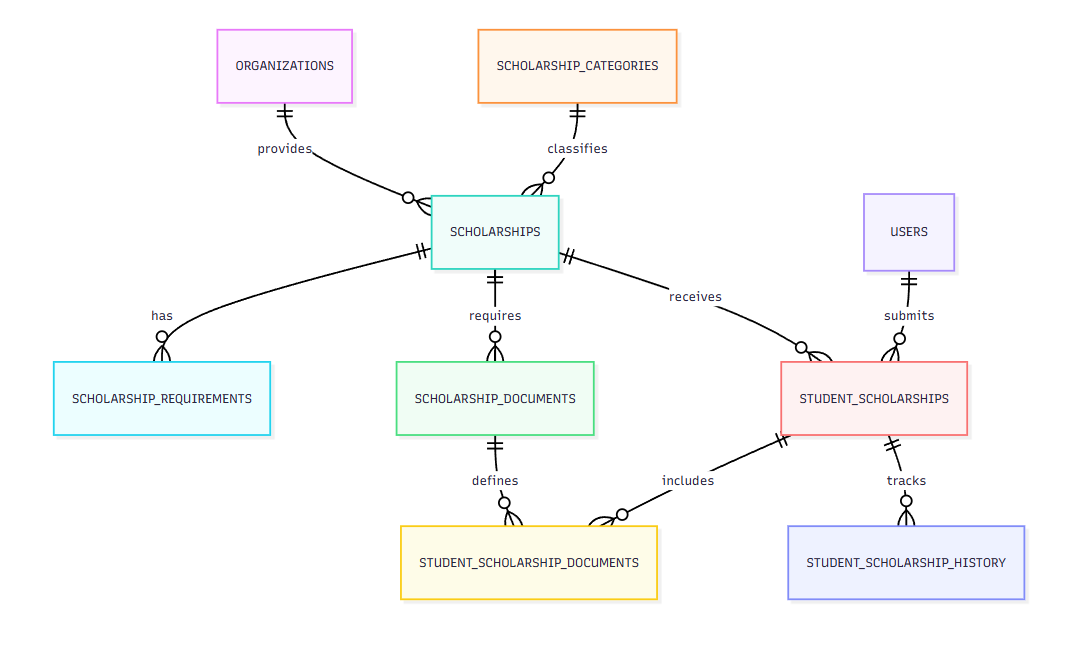
\includegraphics[width=0.9\textwidth]{images/chapter3/scholarship/scholarship-erd.png}%
    }{%
        \rectbox{Sơ đồ ERD cho phân hệ học bổng}
    }
    \caption{Sơ đồ ERD cho phân hệ học bổng}
    \label{fig:erd-scholarship}
\end{figure}

\section{Luồng tương tác giữa các thành phần}
Phần này mô tả ba luồng tương tác tiêu biểu giữa các thành phần kiến trúc, ở góc nhìn thành phần nào tham gia và giao tiếp qua kênh nào; đặc tả chi tiết từng bước nghiệp vụ và endpoint cụ thể của các luồng này được trình bày tại Chương 4.

\subsection{Luồng ghi nhận và phân loại giao dịch bằng AI}
Sinh viên nhập một mô tả giao dịch bằng ngôn ngữ tự nhiên trên Mobile App. Yêu cầu được gửi tới Backend qua HTTP REST; Backend chuyển tiếp sang AI Service để phân loại; AI Service trả về hũ tài chính và danh mục chi tiêu được đề xuất; Backend chuyển kết quả này về Mobile App để sinh viên xác nhận trước khi lưu giao dịch vào PostgreSQL.

\subsection{Luồng trò chuyện AI thời gian thực}
Sinh viên đặt câu hỏi trong màn hình trò chuyện AI. Mobile App mở một kết nối SSE tới Backend; Backend xác thực rồi chuyển tiếp yêu cầu sang AI Service; AI Service suy luận và truy vấn dữ liệu thật qua Backend khi cần, sau đó truyền câu trả lời về dưới dạng luồng token liên tục; Backend chuyển tiếp luồng này về Mobile App để hiển thị theo thời gian thực (Hình~\ref{fig:ai-flow}).

\subsection{Luồng xét duyệt học bổng và thông báo kết quả}
Nhà tài trợ cập nhật trạng thái một hồ sơ ứng tuyển trên Web Admin Portal. Yêu cầu được gửi tới Backend qua HTTP REST; Backend cập nhật trạng thái hồ sơ trong PostgreSQL, sau đó đẩy một tác vụ gửi thông báo vào hàng đợi Redis thay vì gửi ngay trong cùng yêu cầu; một worker chạy nền lấy tác vụ ra khỏi hàng đợi và gọi Firebase Cloud Messaging để gửi thông báo đẩy tới thiết bị của sinh viên.

\section{Đánh giá kiến trúc hệ thống}

\subsection{Ưu điểm}
Kiến trúc phân tán nhiều tầng, đa-repository giúp tách trách nhiệm rõ ràng theo cả chiều tầng (trình bày/ứng dụng/dữ liệu) lẫn chiều dịch vụ (Mobile, Web Admin, Backend, AI Service). Mỗi cặp thành viên trong nhóm có thể phát triển độc lập trên repository riêng của mình, hạn chế xung đột mã nguồn khi làm việc song song (liên kết với cách phân công tại Chương 5). Việc tách AI Service thành một dịch vụ riêng giúp cô lập hoàn toàn rủi ro về độ trễ, lỗi hoặc chi phí gọi mô hình ngôn ngữ lớn khỏi các nghiệp vụ lõi (tài chính, học bổng), đảm bảo các chức năng cốt lõi vẫn hoạt động ổn định ngay cả khi thành phần AI gặp sự cố. Việc xử lý bất đồng bộ qua hàng đợi giúp hệ thống chịu tải tốt khi cần gửi thông báo tới số lượng lớn người dùng cùng lúc mà không làm chậm các yêu cầu API chính.

\subsection{Khả năng mở rộng và bảo trì}
Kiến trúc phân lớp và module hóa theo miền nghiệp vụ cho phép bổ sung dịch vụ hoặc miền nghiệp vụ mới mà không phá vỡ cấu trúc hiện có. Tầng trừu tượng hóa nhà cung cấp mô hình ngôn ngữ lớn tại AI Service cho phép đổi hoặc bổ sung nhà cung cấp mới mà không cần sửa đổi logic nghiệp vụ ở các tầng phía trên. Việc tổ chức đa-repository, mỗi dịch vụ một repository riêng, giúp giảm xung đột mã nguồn giữa các nhóm nhỏ và cho phép mỗi dịch vụ được triển khai, phiên bản hóa độc lập với các dịch vụ còn lại.

\subsection{Hướng mở rộng kiến trúc trong tương lai}
Mã nguồn của AI Service hiện đã chuẩn bị sẵn một khung điều phối đa-agent (multi-agent orchestration), cho phép định tuyến yêu cầu tới nhiều tác nhân AI chuyên biệt theo từng miền nghiệp vụ khác nhau; tuy nhiên khung này chưa được kích hoạt trong luồng xử lý thực tế ở phiên bản hiện tại, mà chỉ mới sử dụng một tác nhân duy nhất với cơ chế phân loại ý định như đã mô tả ở Mục 3.4. Đây là nền tảng sẵn có để hệ thống có thể mở rộng thành kiến trúc đa-agent thực thụ khi bổ sung thêm các nghiệp vụ AI phức tạp hơn trong tương lai.

\subsection{Giới hạn hiện tại}
Nhìn từ góc độ kiến trúc, hệ thống còn một số giới hạn: một số thao tác tài chính tổng hợp (như phân bổ thu nhập vào nhiều hũ cùng lúc) chưa được bọc trong một transaction cơ sở dữ liệu tường minh, tiềm ẩn rủi ro không nhất quán nếu xảy ra lỗi giữa chừng (chi tiết tại Chương 4); hệ thống chưa có bộ benchmark định lượng chính thức, có thể tái lập cho các thành phần AI (chi tiết tại Chương 6); và hệ thống phụ thuộc vào các dịch vụ bên thứ ba nằm ngoài tầm kiểm soát trực tiếp (Firebase Cloud Messaging, nhà cung cấp mô hình ngôn ngữ lớn).


\chapter{Quá trình phát triển và triển khai}
\label{ch:phat-trien-trien-khai}

\section{Phương pháp thực hiện}
Nhóm áp dụng mô hình phát triển phần mềm linh hoạt \textbf{Agile/Scrum} xuyên suốt quá trình thực hiện đồ án thay vì phát triển tuần tự theo kiểu Waterfall truyền thống. Công việc được chia thành các chu kỳ lặp (sprint) ngắn kéo dài \textbf{1 tuần}, mỗi sprint tập trung hoàn thiện một nhóm chức năng cụ thể thay vì dàn trải toàn bộ hệ thống cùng lúc.

Để đảm bảo quy chuẩn và tiến độ, nhóm thiết lập bảng vận hành Scrum với các yếu tố cốt lõi:
\begin{itemize}
    \item \textbf{Vai trò (Actor):} Phân định rõ Product Owner (đại diện nghiệp vụ), Scrum Master (điều phối tiến trình) và Development Team.
    \item \textbf{Sự kiện (Ceremony):} Tổ chức Sprint Planning đầu tuần, Daily Standup hàng ngày, và Sprint Review / Retrospective cuối mỗi tuần để đánh giá kết quả và cải tiến.
    \item \textbf{Tạo tác (Artifact):} Quản lý Product Backlog, Sprint Backlog và các Increment (sản phẩm tăng trưởng) có giá trị sau mỗi sprint.
    \item \textbf{Tiêu chuẩn (DoR/DoD \& Acceptance Criteria):} 
    \begin{itemize}
        \item \textit{Definition of Ready (DoR):} Yêu cầu/user story phải có mô tả rõ ràng, đầy đủ Acceptance Criteria và được thiết kế UI/UX hoàn chỉnh trước khi đưa vào Sprint.
        \item \textit{Definition of Done (DoD):} Code phải vượt qua các bài kiểm tra tự động (unit test), không có lỗi linter, được review chéo bởi ít nhất một thành viên khác và tích hợp thành công không gây lỗi trên môi trường staging.
    \end{itemize}
\end{itemize}

Thông qua việc theo dõi biểu đồ tiến độ (milestone thực tế so với kế hoạch), \textit{velocity} (tốc độ hoàn thành story points) và \textit{defect leakage} (tỷ lệ lỗi lọt ra ngoài sprint), nhóm có thể kiểm soát và sớm phát hiện rủi ro kỹ thuật. Điển hình, 3 sự cố lớn liên quan đến AI (phân loại sai giao dịch, Prompt Injection, timeout khi xử lý dữ liệu) đã được liên kết trực tiếp vào backlog và giải quyết dứt điểm trong các sprint ở giai đoạn 3 và 4, thay vì để tồn đọng đến cuối dự án.

\section{Công cụ hỗ trợ và Quy trình CI/CD}
\subsection{Công cụ hỗ trợ phát triển}
Để phối hợp làm việc nhóm và quản lý mã nguồn hiệu quả trong suốt quá trình phát triển, nhóm sử dụng các công cụ:
\begin{itemize}
    \item \textbf{Git/GitHub:} Mỗi dịch vụ (Backend, AI Service, Mobile App, Web Admin Portal) có một repository riêng, quản lý phiên bản độc lập. Trong mỗi repo, mỗi tính năng được phát triển trên một nhánh (feature branch) riêng và được xem xét qua cơ chế Pull Request.
    \item \textbf{Jira:} Quản lý backlog, phân chia công việc theo từng sprint 1 tuần và theo dõi tiến độ hoàn thành của từng thành viên.
    \item \textbf{Slack/Zalo:} Kênh trao đổi chính, dùng để họp trực tuyến định kỳ, thông báo tiến độ và xử lý vướng mắc.
    \item \textbf{Google Drive:} Lưu trữ tài liệu chung như đề cương, tài liệu đặc tả, hình ảnh thiết kế.
\end{itemize}

\subsection{Quy trình Tích hợp và Triển khai liên tục (CI/CD)}
Dựa trên cấu hình Jenkins thực tế của hệ thống, quy trình CI/CD được thiết lập tự động hóa nhằm giảm thiểu sai sót:
\begin{itemize}
    \item \textbf{CI Pipeline (Kiểm tra và Build):} Khi có Pull Request mới, Jenkins tự động \textit{checkout} mã nguồn, cài đặt thư viện (\texttt{npm install}), chạy quá trình build (\texttt{npm run build}) để phát hiện lỗi biên dịch. Sau đó, mã nguồn được đóng gói thành \textbf{Docker Image} với tag tương ứng. (Theo cấu trúc chuẩn, quy trình bao gồm cả các bước \textit{lint}, \textit{unit test}, \textit{build} và \textit{security scan}).
    \item \textbf{CD Pipeline (Triển khai - Deploy):} Khi mã nguồn được merge vào nhánh chính (\texttt{staging} hoặc \texttt{main}), pipeline CD sẽ đồng bộ mã nguồn, yêu cầu xác nhận thủ công (Manual Approval) từ người quản lý trước khi triển khai. Sau khi xác nhận, hệ thống nạp các biến môi trường (\texttt{.env.docker}), tắt các container hiện tại và khởi tạo container mới thông qua \texttt{docker compose build} và \texttt{docker compose up -d}. Quá trình deploy staging thành công sẽ là bước đệm trước khi đưa lên production.
\end{itemize}

\textbf{Tiêu chí Rollback (Phục hồi phiên bản):} Để đảm bảo tính sẵn sàng, hệ thống quy định các tiêu chí kích hoạt rollback như sau:
\begin{itemize}
    \item \textit{Smoke test thất bại:} Ứng dụng không phản hồi hoặc container bị crash liên tục sau khi khởi động.
    \item \textit{Lỗi hệ thống tăng đột biến:} Tỷ lệ lỗi (error rate) giám sát được trên production tăng bất thường ngay sau khi triển khai phiên bản mới.
    \item Khi thỏa mãn tiêu chí, quản trị viên sẽ từ chối release (hoặc kích hoạt job rollback) để hệ thống tự động kéo lại tag Docker Image của phiên bản ổn định trước đó và khởi động lại dịch vụ.
\end{itemize}

\section{Tổ chức nhóm và phân công chuyên môn}
Nhóm gồm 6 thành viên, được chia thành 3 cặp phụ trách song song 3 mảng chức năng chính của hệ thống, mỗi cặp đảm nhận trọn vẹn cả phần giao diện (Frontend) lẫn xử lý nghiệp vụ phía máy chủ (Backend) cho mảng của mình nhằm đảm bảo tính liền mạch khi tích hợp. 

\begin{table}[H]
    \centering
    \begin{tabular}{|L{5cm}|L{9cm}|}
        \hline
        \textbf{Thành viên phụ trách} & \textbf{Mảng chức năng / Phạm vi công việc} \\
        \hline
        Võ Hoàng Nguyên, Nguyễn Duy Lâm & Mô-đun Tài chính 6 lọ (6 Jars) -- Frontend Mobile và Backend API. \\ \hline
        Nguyễn Thành Nhật, Huỳnh Công Minh & Hệ thống thông báo (Notification) và các luồng thông tin người dùng cơ bản -- Frontend Mobile và Backend API. \\ \hline
        Nguyễn Vĩnh Lương, Huỳnh Tấn Lộc & Quản lý học bổng và trang quản trị Webadmin học bổng -- Frontend (Mobile/Webadmin) và Backend API. Huỳnh Tấn Lộc phụ trách thêm DevOps. \\
        \hline
    \end{tabular}

    \caption{Phân công chuyên môn theo mảng chức năng}
    \label{tab:phan-cong}
\end{table}

Nhằm khắc phục tình trạng \textit{knowledge silo} (chia cắt kiến thức) do phân công theo cặp và giảm thiểu rủi ro khi có thành viên vắng mặt, nhóm áp dụng:
\begin{itemize}
    \item \textbf{Ma trận RACI \& Code Ownership:} Định nghĩa rõ ràng ai chịu trách nhiệm chính (Responsible) và ai phê duyệt (Accountable) cho từng tính năng, không để chồng chéo quyền hạn.
    \item \textbf{Review chéo (Cross-review):} Các Pull Request của một cặp bắt buộc phải được review và approve bởi ít nhất một thành viên từ cặp khác. Quá trình này giúp phát hiện lỗi khách quan và phân tán hiểu biết về code.
    \item \textbf{Knowledge Sharing Sessions (Phiên chia sẻ kiến thức):} Được tổ chức định kỳ sau mỗi sprint để chia sẻ về kiến trúc hệ thống, các luồng tích hợp API phức tạp và đặc biệt là kinh nghiệm xử lý AI, đảm bảo mọi người đều có khả năng \textit{backup} lẫn nhau khi cần thiết.
\end{itemize}

\section{Các giai đoạn phát triển}
Đồ án được thực hiện trong khoảng thời gian từ ngày 24/08/2025 đến ngày 21/07/2026, chia thành 5 giai đoạn chính như sau:
\begin{itemize}
    \item \textbf{Giai đoạn 1 -- Khảo sát và thiết kế hệ thống (24/08/2025 -- 09/2025):} Khảo sát thực trạng các ứng dụng quản lý tài chính và kết nối học bổng hiện có, xác định phạm vi đề tài, thiết kế kiến trúc tổng thể và cơ sở dữ liệu, hoàn thiện đề cương chi tiết.
    \item \textbf{Giai đoạn 2 -- Xây dựng nền tảng cốt lõi (10/2025 -- 01/2026):} Triển khai song song ba mảng chức năng cốt lõi theo phân công tại Bảng~\ref{tab:phan-cong}: mô-đun Tài chính 6 lọ, hệ thống thông báo và luồng người dùng cơ bản, quản lý học bổng và Webadmin. Mỗi mảng được phát triển theo các sprint ngắn, review chéo qua Pull Request trên GitHub.
    \item \textbf{Giai đoạn 3 -- Tích hợp trí tuệ nhân tạo (02/2026 -- 04/2026):} Bắt đầu xây dựng AI Service (FastAPI kết hợp LangChain và Gemini API), tích hợp trợ lý ảo AI Chat, bộ phân loại giao dịch tự động và cơ chế gợi ý học bổng vào các mảng chức năng đã hoàn thiện ở Giai đoạn 2.
    \item \textbf{Giai đoạn 4 -- Hoàn thiện, tối ưu và triển khai (05/2026 -- 06/2026):} Tối ưu hiệu năng và bảo mật (chuẩn hóa Unicode tiếng Việt, chống Prompt Injection), kiểm thử toàn diện hệ thống, cấu hình build và deploy ứng dụng lên môi trường thật.
    \item \textbf{Giai đoạn 5 -- Hoàn thiện báo cáo và bảo vệ (07/2026 -- 21/07/2026):} Tổng hợp kết quả đạt được, hoàn chỉnh báo cáo khóa luận, chuẩn bị slide và demo phục vụ báo cáo trước Hội đồng.
\end{itemize}

\section{Các thách thức và giải pháp thực hiện}
Trong suốt quá trình phát triển và tích hợp hệ thống Student360, bên cạnh các vấn đề về mặt kỹ thuật, nhóm phát triển còn đối mặt với các khó khăn thách thức lớn liên quan đến yếu tố con người và sự phối hợp giữa các nhóm. Dưới đây là các thách thức cốt lõi và các giải pháp thực tế được áp dụng:

\subsection{Thách thức ở tầng trình bày di động (Mobile App)}
\begin{itemize}
    \item \textbf{Thách thức 1 -- Truyền phản hồi AI theo thời gian thực:} Do cơ chế tải dữ liệu tuần tự trên nền di động không ổn định như trên trình duyệt, việc chờ nhận đủ toàn bộ phản hồi từ mô hình ngôn ngữ lớn (Gemini AI) trước khi hiển thị tạo ra độ trễ lớn, ảnh hưởng tiêu cực đến trải nghiệm người dùng (UX).
    \item \textit{Giải pháp:} Ứng dụng cơ chế đọc dữ liệu tăng dần theo từng phần (Streaming / Server-Sent Events - SSE). Mobile App đọc dữ liệu dạng chunk và cập nhật giao diện tức thời ngay khi nhận được ký tự đầu tiên, giúp giảm cảm giác chờ đợi của sinh viên.
    \item \textbf{Thách thức 2 -- Đồng bộ dữ liệu và tính nhất quán giữa các màn hình:} Một giao dịch chi tiêu mới của sinh viên ảnh hưởng đồng thời đến nhiều giao diện độc lập (số dư các hũ 6 lọ, lịch sử giao dịch gần đây, biểu đồ báo cáo tài chính và các cảnh báo chi tiêu). Việc tự cộng trừ số liệu thủ công ở các màn hình khác nhau dễ dẫn đến sai lệch dữ liệu.
    \item \textit{Giải pháp:} Sử dụng cơ chế Query Invalidation của thư viện React Query. Frontend tự động đánh dấu toàn bộ các nhóm dữ liệu tài chính liên quan là đã lỗi thời ngay sau khi Backend ghi nhận giao dịch thành công, buộc hệ thống tự động tải lại dữ liệu ngầm và cập nhật UI đồng bộ mà không cần tải lại toàn bộ ứng dụng.
\end{itemize}

\subsection{Thách thức ở tầng AI và Bảo mật (AI Service \& Backend)}
\begin{itemize}
    \item \textbf{Thách thức 3 -- Độ trễ lớn khi gọi LLM và xử lý tiếng Việt:} Thời gian phản hồi trung bình của chatbot AI khoảng 4 giây, có thể lên tới hơn 10 giây đối với câu hỏi phức tạp. Đồng thời, việc sinh viên nhập từ viết tắt, tiếng lóng tiếng Việt hoặc lỗi Unicode không đồng nhất (NFC/NFD) làm giảm độ chính xác của bộ phân loại giao dịch.
    \item \textit{Giải pháp:} Áp dụng bộ lọc chuẩn hóa Unicode NFC ở Backend trước khi gửi yêu cầu sang AI Service. Đồng thời, thiết lập cơ chế phân loại hỗn hợp (Hybrid Classification Pipeline): kiểm tra danh mục từ khóa cá nhân hóa trong cơ sở dữ liệu trước với độ trễ 0ms; chỉ khi không khớp mới gọi LLM để suy luận ngữ nghĩa.
    \item \textbf{Thách thức 4 -- Ngăn chặn tấn công Prompt Injection và rò rỉ dữ liệu:} Người dùng có thể cố tình nhập câu lệnh tiêm nhiễm để phá vỡ ngữ cảnh an toàn của trợ lý AI, hoặc giả mạo ID người dùng (\texttt{user\_id}) trong request API để truy cập thông tin tài chính của sinh viên khác.
    \item \textit{Giải pháp:} Xây dựng chính sách bảo mật hai tầng (Policy Filter) trên AI Service để phát hiện và chặn đứng các câu lệnh tiêm nhiễm độc hại. Ở phía Backend, hệ thống tự động ghi đè tham số \texttt{user\_id} của mọi yêu cầu bằng thông tin lấy từ token JWT đã được xác thực, ngăn chặn hoàn toàn nguy cơ client tự truyền ID tự do.
\end{itemize}

\subsection{Thách thức về yếu tố con người và phối hợp liên nhóm}
\begin{itemize}
    \item \textbf{Thách thức 5 -- Rào cản giao tiếp và nguy cơ đứt gãy thông tin trong tập thể lớn:} 
    Với quy mô dự án lên tới 14 thành viên chia làm 3 nhóm độc lập, luồng thông tin giao tiếp phình to theo cấp số nhân. Nhóm phát triển phân hệ Tài chính (6 thành viên) liên tục đối mặt với việc "nhiễu" thông tin trên các kênh trao đổi chung. Các quyết định kỹ thuật hoặc thay đổi về mặt nghiệp vụ thường bị trôi hoặc hiểu sai lệch giữa các nhóm nếu không được truyền đạt rõ ràng, dẫn đến tình trạng không đồng nhất về hiểu biết hệ thống (Information Asymmetry).
    
    \item \textbf{Thách thức 6 -- Khó khăn trong việc thống nhất kiến trúc và các mô-đun dùng chung (Shared Services):} 
    Do hệ thống chia làm 3 phân hệ hoạt động trên cùng một nền tảng cơ sở dữ liệu và hạ tầng, các chức năng dùng chung như xác thực người dùng (Authentication/Authorization), hệ thống thông báo đẩy (Notification), cài đặt ứng dụng (Setup), và cấu hình hệ thống (Configuration) trở thành các điểm thắt cổ chai (bottlenecks). Việc thống nhất kiểu dữ liệu, cấu trúc DB và đặc tả API của các phần chung này đòi hỏi sự thương thảo kéo dài giữa cả 3 nhóm. Bất kỳ sự tự ý điều chỉnh nào ở một nhóm cũng có thể trực tiếp làm đổ vỡ (break) chức năng của hai nhóm còn lại.
    
    \item \textbf{Thách thức 7 -- Sự phụ thuộc chéo giữa các tính năng (Feature Dependency) và trễ tiến độ dây chuyền:} 
    Phân hệ Tài chính có sự phụ thuộc rất lớn vào các phân hệ khác (ví dụ: cần luồng đăng nhập thành công của phân hệ lõi để lấy thông tin sinh viên, và cần hệ thống thông báo để gửi cảnh báo chi tiêu). Khi các nhóm có tốc độ phát triển không đồng đều hoặc một nhóm gặp sự cố kỹ thuật dẫn đến chậm trễ tiến độ (delay), toàn bộ chuỗi tích hợp của phân hệ Tài chính cũng bị đình trệ theo. Việc quản lý sự phụ thuộc này trong mô hình phát triển song song cực kỳ phức tạp.
    
    \item \textbf{Thách thức 8 -- Xung đột mã nguồn và bất đồng bộ trong quy trình triển khai (Git Conflict \& Release Management):} 
    Với 14 lập trình viên cùng đẩy mã nguồn lên các repository cốt lõi của hệ thống (như Backend NestJS và Frontend Mobile), tần suất xảy ra xung đột code (code conflict) rất cao. Việc thiếu thống nhất trong quy chuẩn viết code (coding convention), quy trình đặt tên nhánh (Git branch naming) hay thời điểm merge code lên các nhánh \texttt{staging}/\texttt{main} gây khó khăn lớn cho việc kiểm soát phiên bản và triển khai tự động (CI/CD).

    \item \textit{Giải pháp thực hiện:} Để giải quyết triệt để các thách thức về mặt con người và quy trình phối hợp trên, các nhóm đã cùng thống nhất và áp dụng đồng bộ các giải pháp sau:
    \begin{itemize}
        \item \textit{Chuẩn hóa kênh và tần suất giao tiếp:} Thiết lập các kênh thảo luận chuyên biệt cho từng chủ đề nghiệp vụ trên Slack/Zalo. Định kỳ tổ chức các cuộc họp giao ban liên nhóm (Cross-team Sync Meeting) hàng tuần để đại diện các nhóm báo cáo tiến độ, chỉ ra các điểm phụ thuộc chéo và cùng đưa ra quyết định chung bằng văn bản.
        \item \textit{Thiết kế và đóng băng đặc tả API trước khi lập trình:} Sử dụng công cụ Swagger/OpenAPI để định nghĩa chi tiết các API endpoints dùng chung. Bất kỳ sự thay đổi nào về cấu trúc request/response phải được đăng ký qua một biểu mẫu yêu cầu thay đổi (RFC - Request for Comments) và chỉ được áp dụng khi có sự đồng thuận từ đại diện của cả 3 nhóm.
        \item \textit{Quy hoạch rõ ranh giới trách nhiệm (RACI Matrix):} Phân định rõ ràng nhóm nào chịu trách nhiệm phát triển chính và nhóm nào chịu trách nhiệm tích hợp đối với từng API hoặc màn hình dùng chung, tránh việc đùn đẩy trách nhiệm hoặc làm trùng lặp công việc.
        \item \textit{Thống nhất quy trình Git Flow và rà soát mã nguồn liên nhóm (Cross-review):} Áp dụng quy chuẩn viết mã chung (Linter/Prettier) trên toàn bộ dự án. Các Pull Request liên quan đến các mô-đun dùng chung bắt buộc phải nhận được sự kiểm duyệt (approve) của ít nhất một thành viên đại diện cho mỗi nhóm trước khi được phép merge.
        \item \textit{Tận dụng tối đa môi trường Staging chung:} Mọi phiên bản mã nguồn trước khi đưa lên production đều phải được tích hợp và kiểm thử tự động trên môi trường Staging độc lập. Điều này giúp cô lập các lỗi tích hợp sớm và đảm bảo sự cố ở một phân hệ không làm gián đoạn công việc của các phân hệ khác.
    \end{itemize}
\end{itemize}


\chapter{Kiểm thử và đánh giá hệ thống}
\label{ch:hien-thuc-kiem-thu-danh-gia}
\section{Môi trường triển khai và công nghệ sử dụng}
Hệ thống Student360 được hiện thực hóa và kiểm thử trên môi trường cục bộ và nền tảng điện toán đám mây với các thông số cấu hình cụ thể như sau:
\begin{sloppypar}
\begin{itemize}
    \item \textbf{Môi trường máy chủ Backend:} Node.js v20+, NestJS v10.4.20 \cite{nestjs-docs}, TypeORM v0.3.26 \cite{typeorm-docs}.
    \item \textbf{Môi trường máy chủ AI:} Python v3.12, FastAPI v0.115.0 \cite{fastapi-docs}, \texttt{langchain-core} v0.3.0+ \cite{langchain-docs}, Uvicorn v0.30.0.
    \item \textbf{Công nghệ cơ sở dữ liệu:} PostgreSQL 17, \cite{postgresql-docs}, Redis 8 \cite{redis-docs} (làm cache và message broker cho BullMQ \cite{bullmq-docs}).
    \item \textbf{Môi trường Mobile App:} Expo SDK v54 (React Native v0.81) \cite{reactnative-expo}, kết hợp Tamagui v1.135 cho hệ thống Design System.
    \item \textbf{Môi trường Webadmin:} React JS v19.2, Material UI (MUI) v7.3, Vite v7.2.
    \item \textbf{Mô hình AI:} Google Gemini 2.5 Flash / Pro (thông qua Vertex AI API) \cite{gemini-api}.
\end{itemize}
\end{sloppypar}

\section{Các chức năng hệ thống}
\subsection{Ứng dụng di động dành cho sinh viên}
Giao diện ứng dụng di động được thiết kế hướng tới sự trực quan và tối ưu hóa trải nghiệm người dùng (UX) cho đối tượng sinh viên. Dưới đây là các màn hình chính của phân hệ di động:

\begin{figure}[H]
    \noindent\textbf{1.} \textbf{Tổng quan ví:} Màn hình này cung cấp cái nhìn toàn cảnh về tình hình tài chính của sinh viên theo mô hình 6 hũ. Sinh viên có thể nhanh chóng nắm bắt số dư tổng, số dư của từng lọ và biểu đồ xu hướng chi tiêu để điều phối dòng tiền hợp lý.
    
    \vspace{0.2cm}
    \centering
    \begin{minipage}{0.44\textwidth}
        \centering
        \IfFileExists{images/chapter4/mobile/wallet-overview.png}{%
            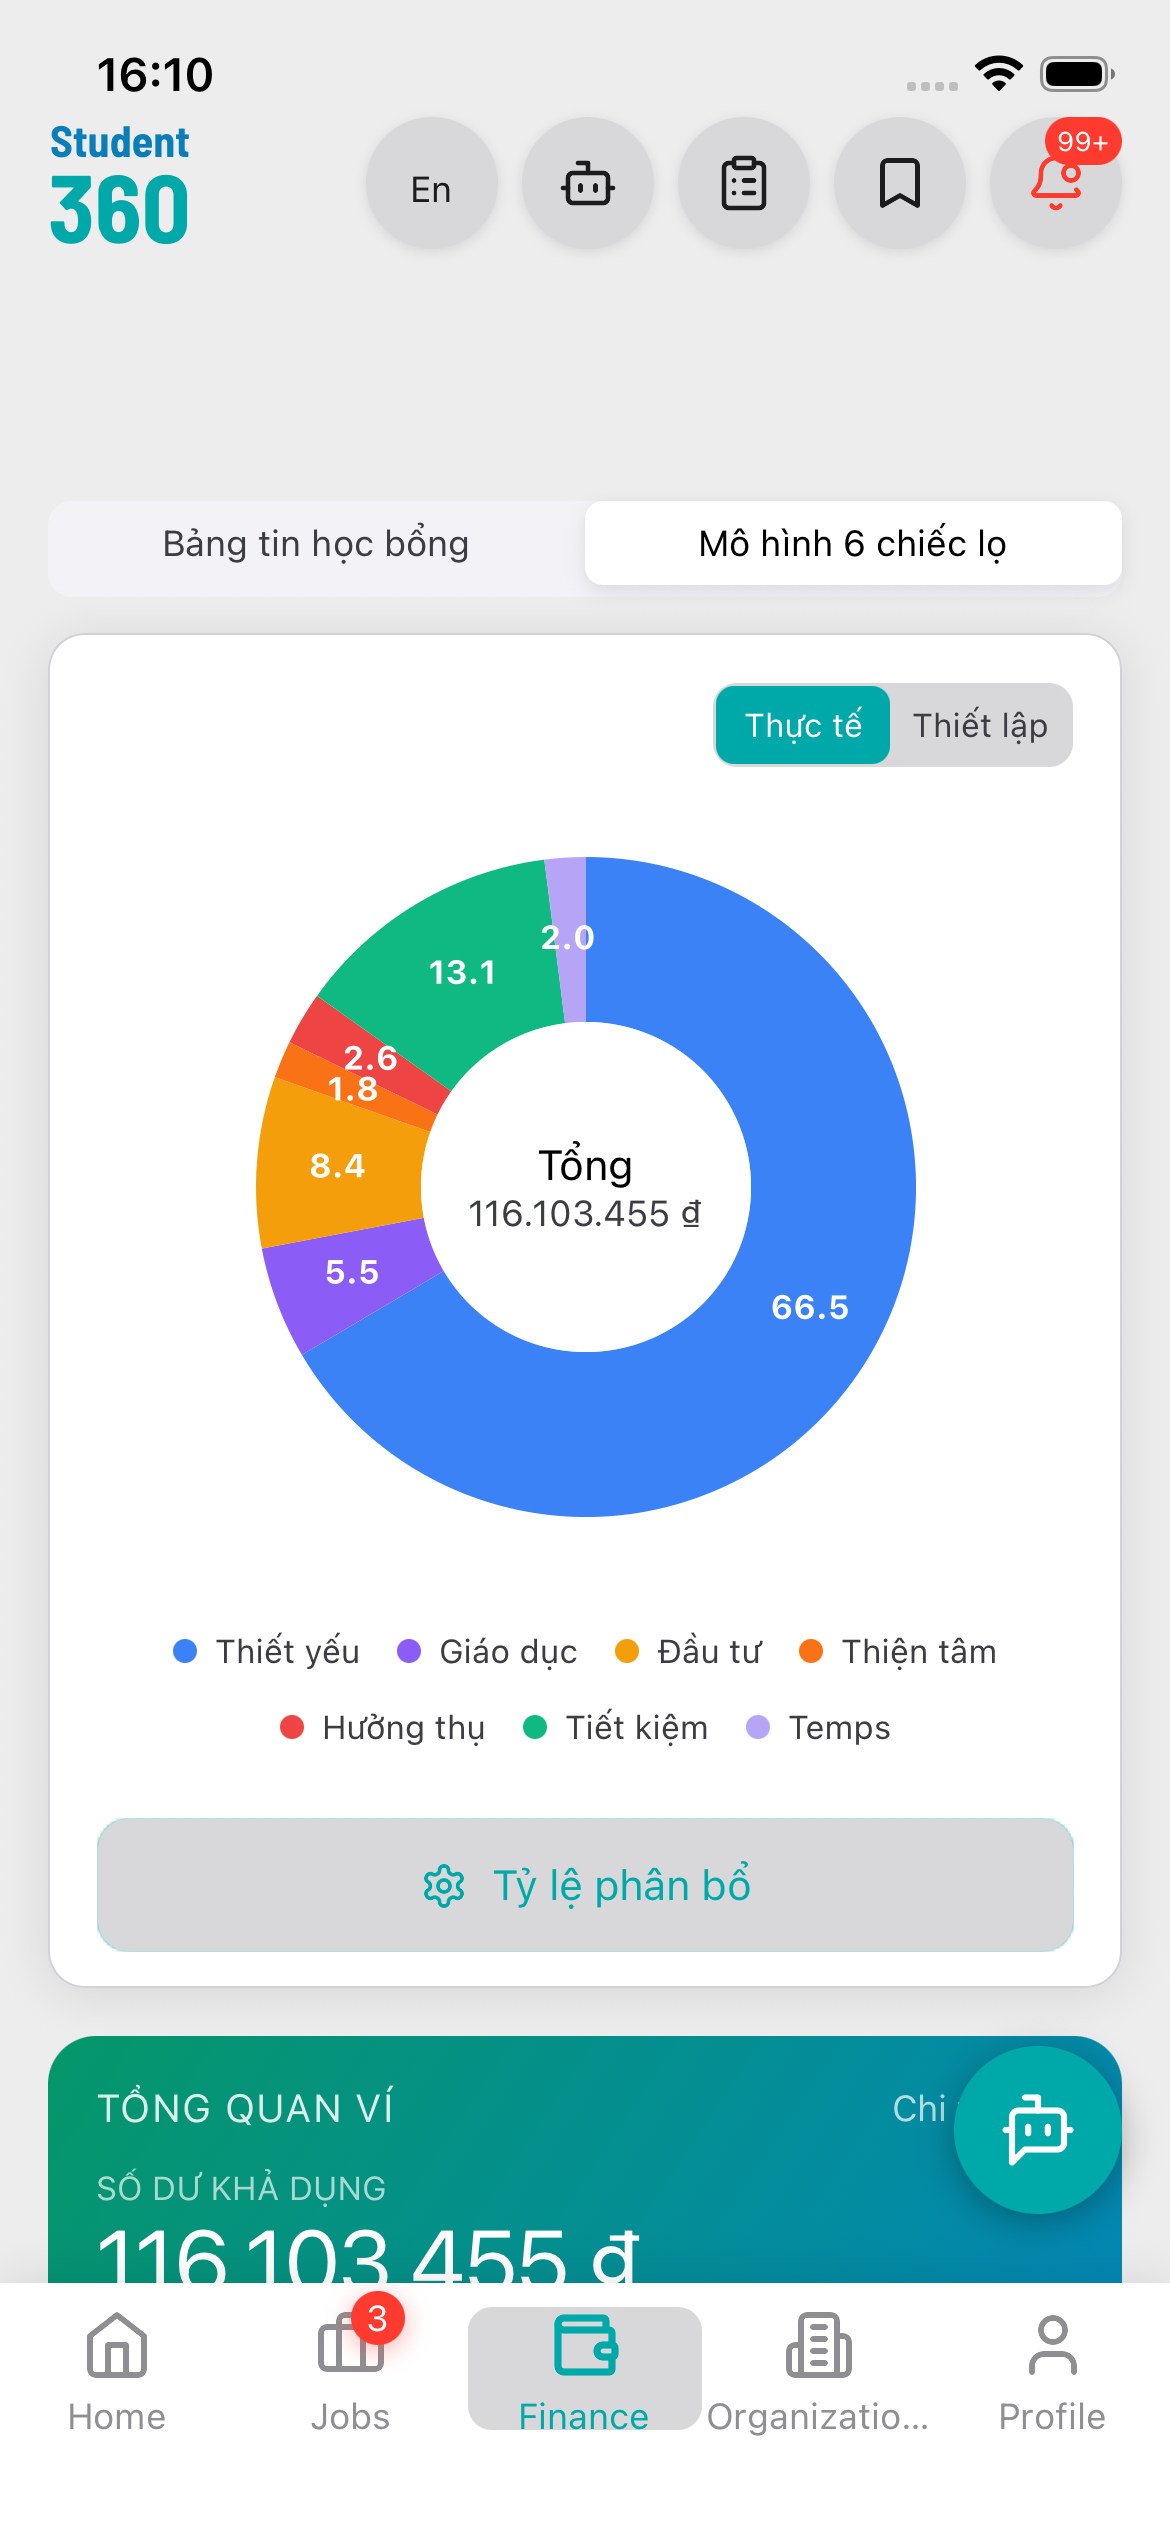
\includegraphics[width=\textwidth]{images/chapter4/mobile/wallet-overview.png}%
        }{%
            \rectbox{Hình ảnh ví 6 lọ tài chính trên Mobile}
        }
        \caption{Giao diện tổng quan ví 6 lọ trên thiết bị di động}
        \label{fig:mobile-6jars}
    \end{minipage}
    \hfill
    \begin{minipage}{0.44\textwidth}
        \centering
        \IfFileExists{images/chapter4/mobile/wallet-overview-detail.png}{%
            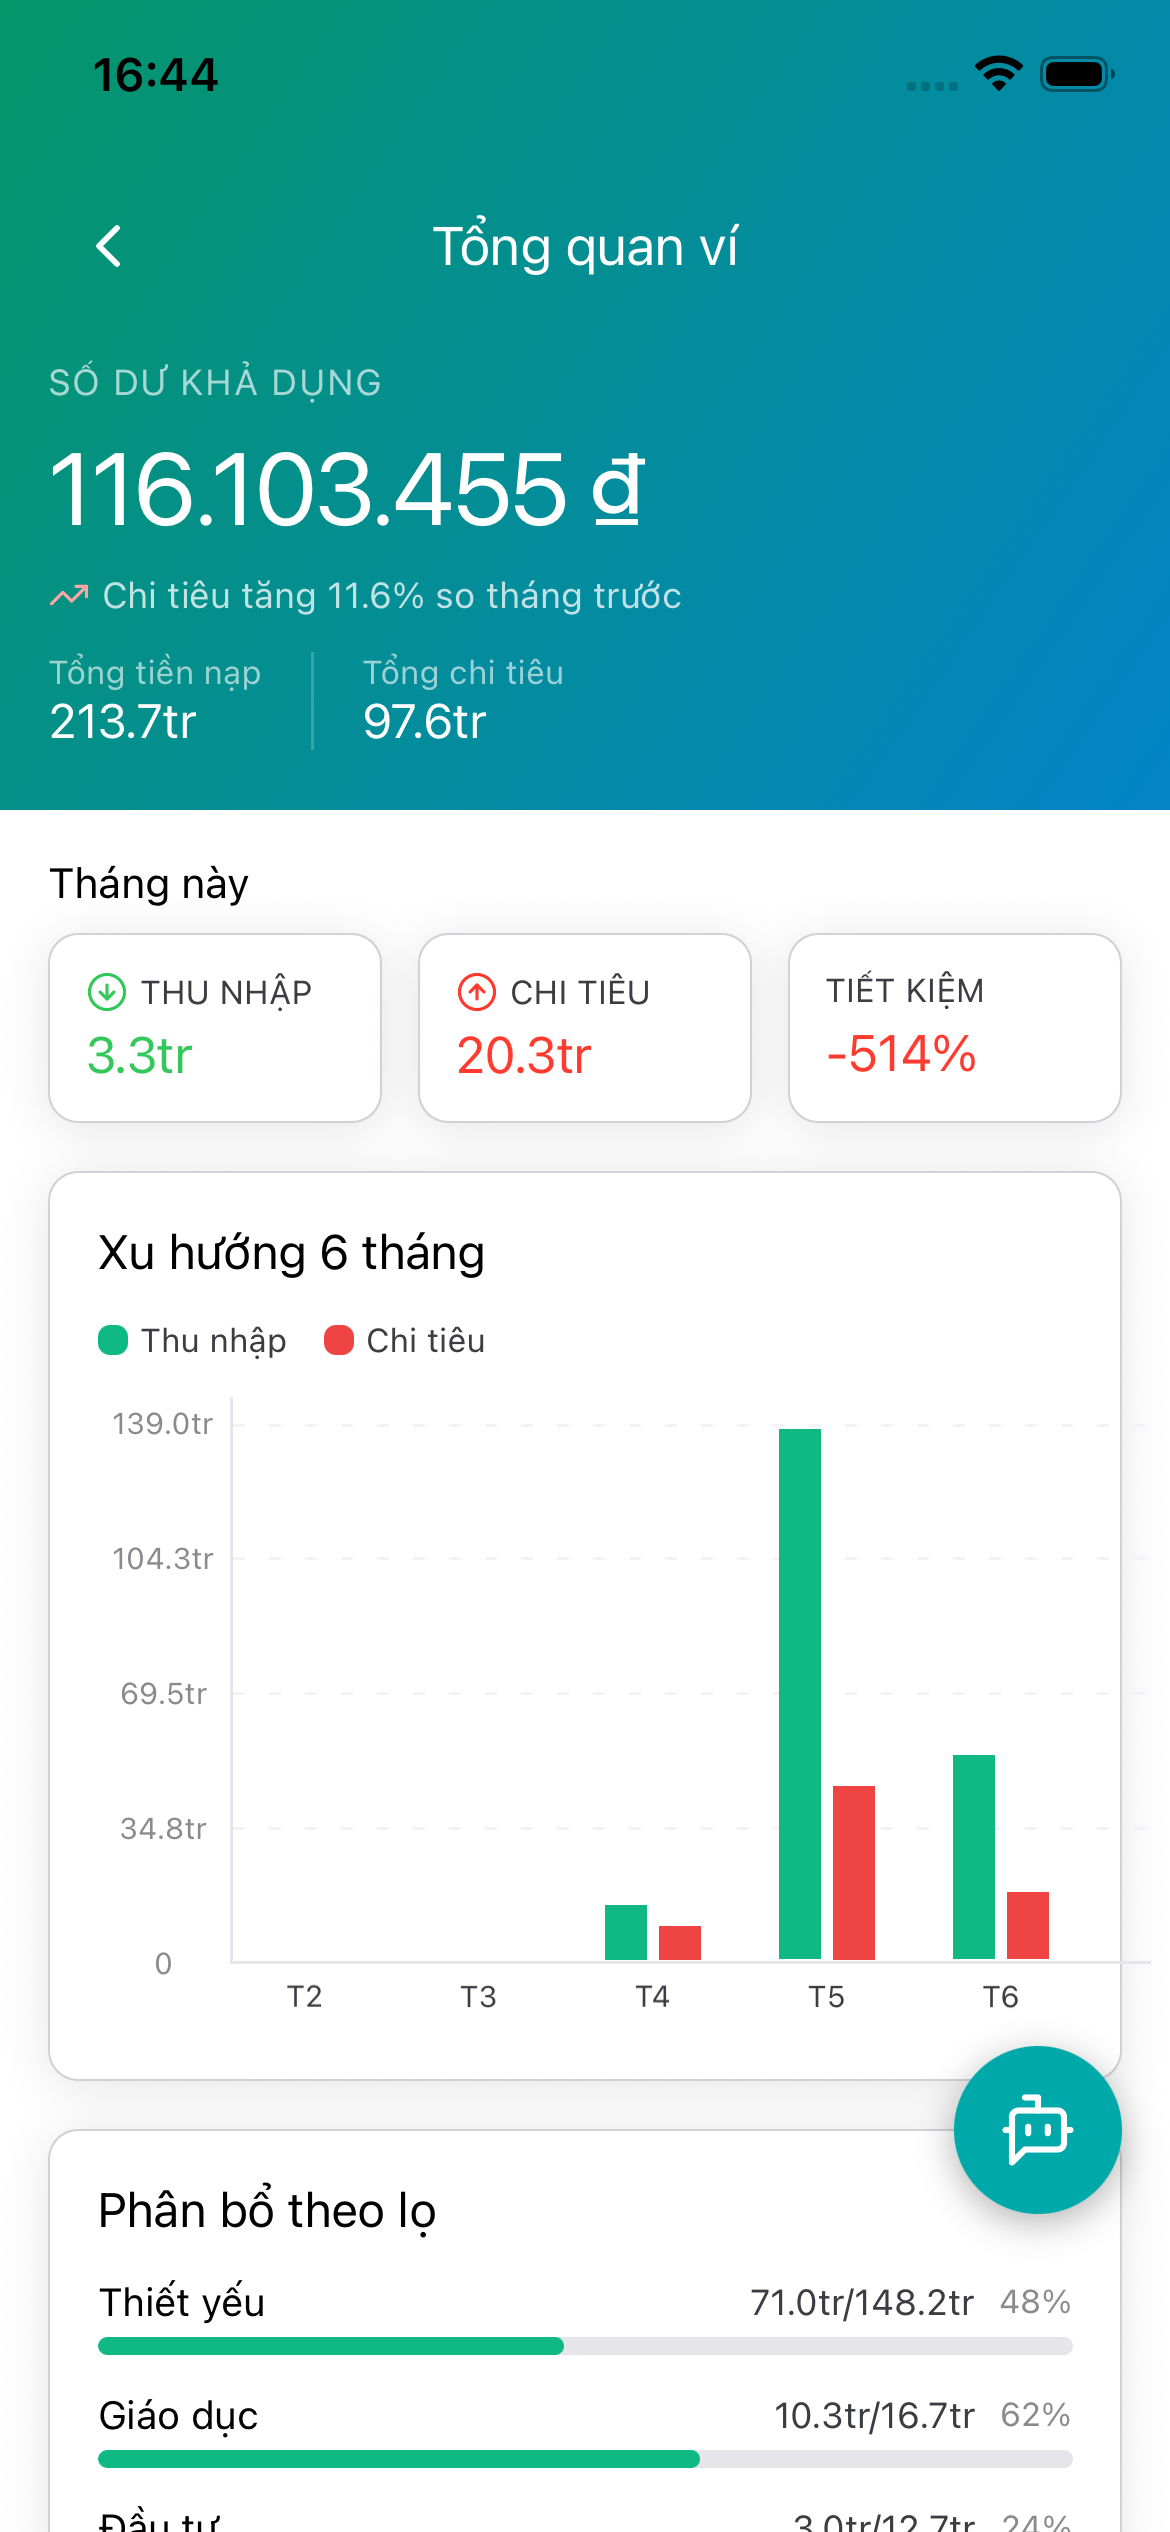
\includegraphics[width=\textwidth]{images/chapter4/mobile/wallet-overview-detail.png}%
        }{%
            \rectbox{Hình ảnh chi tiết xu hướng thu chi trên màn hình ví}
        }
        \caption{Xu hướng thu chi và phân bổ theo lọ trên màn hình tổng quan ví}
        \label{fig:mobile-wallet-detail}
    \end{minipage}
\end{figure}

\begin{figure}[H]
    \noindent\textbf{2.} \textbf{Chi tiết hũ:} Màn hình này hiển thị chi tiết số dư, lịch sử giao dịch và cấu hình riêng biệt của từng hũ tài chính. Sinh viên có thể chủ động cài đặt các mức cảnh báo chi tiêu vượt ngưỡng tại đây để kiểm soát dòng tiền tốt hơn.
    
    \vspace{0.2cm}
    \centering
    \IfFileExists{images/chapter4/mobile/jar-detail.png}{%
        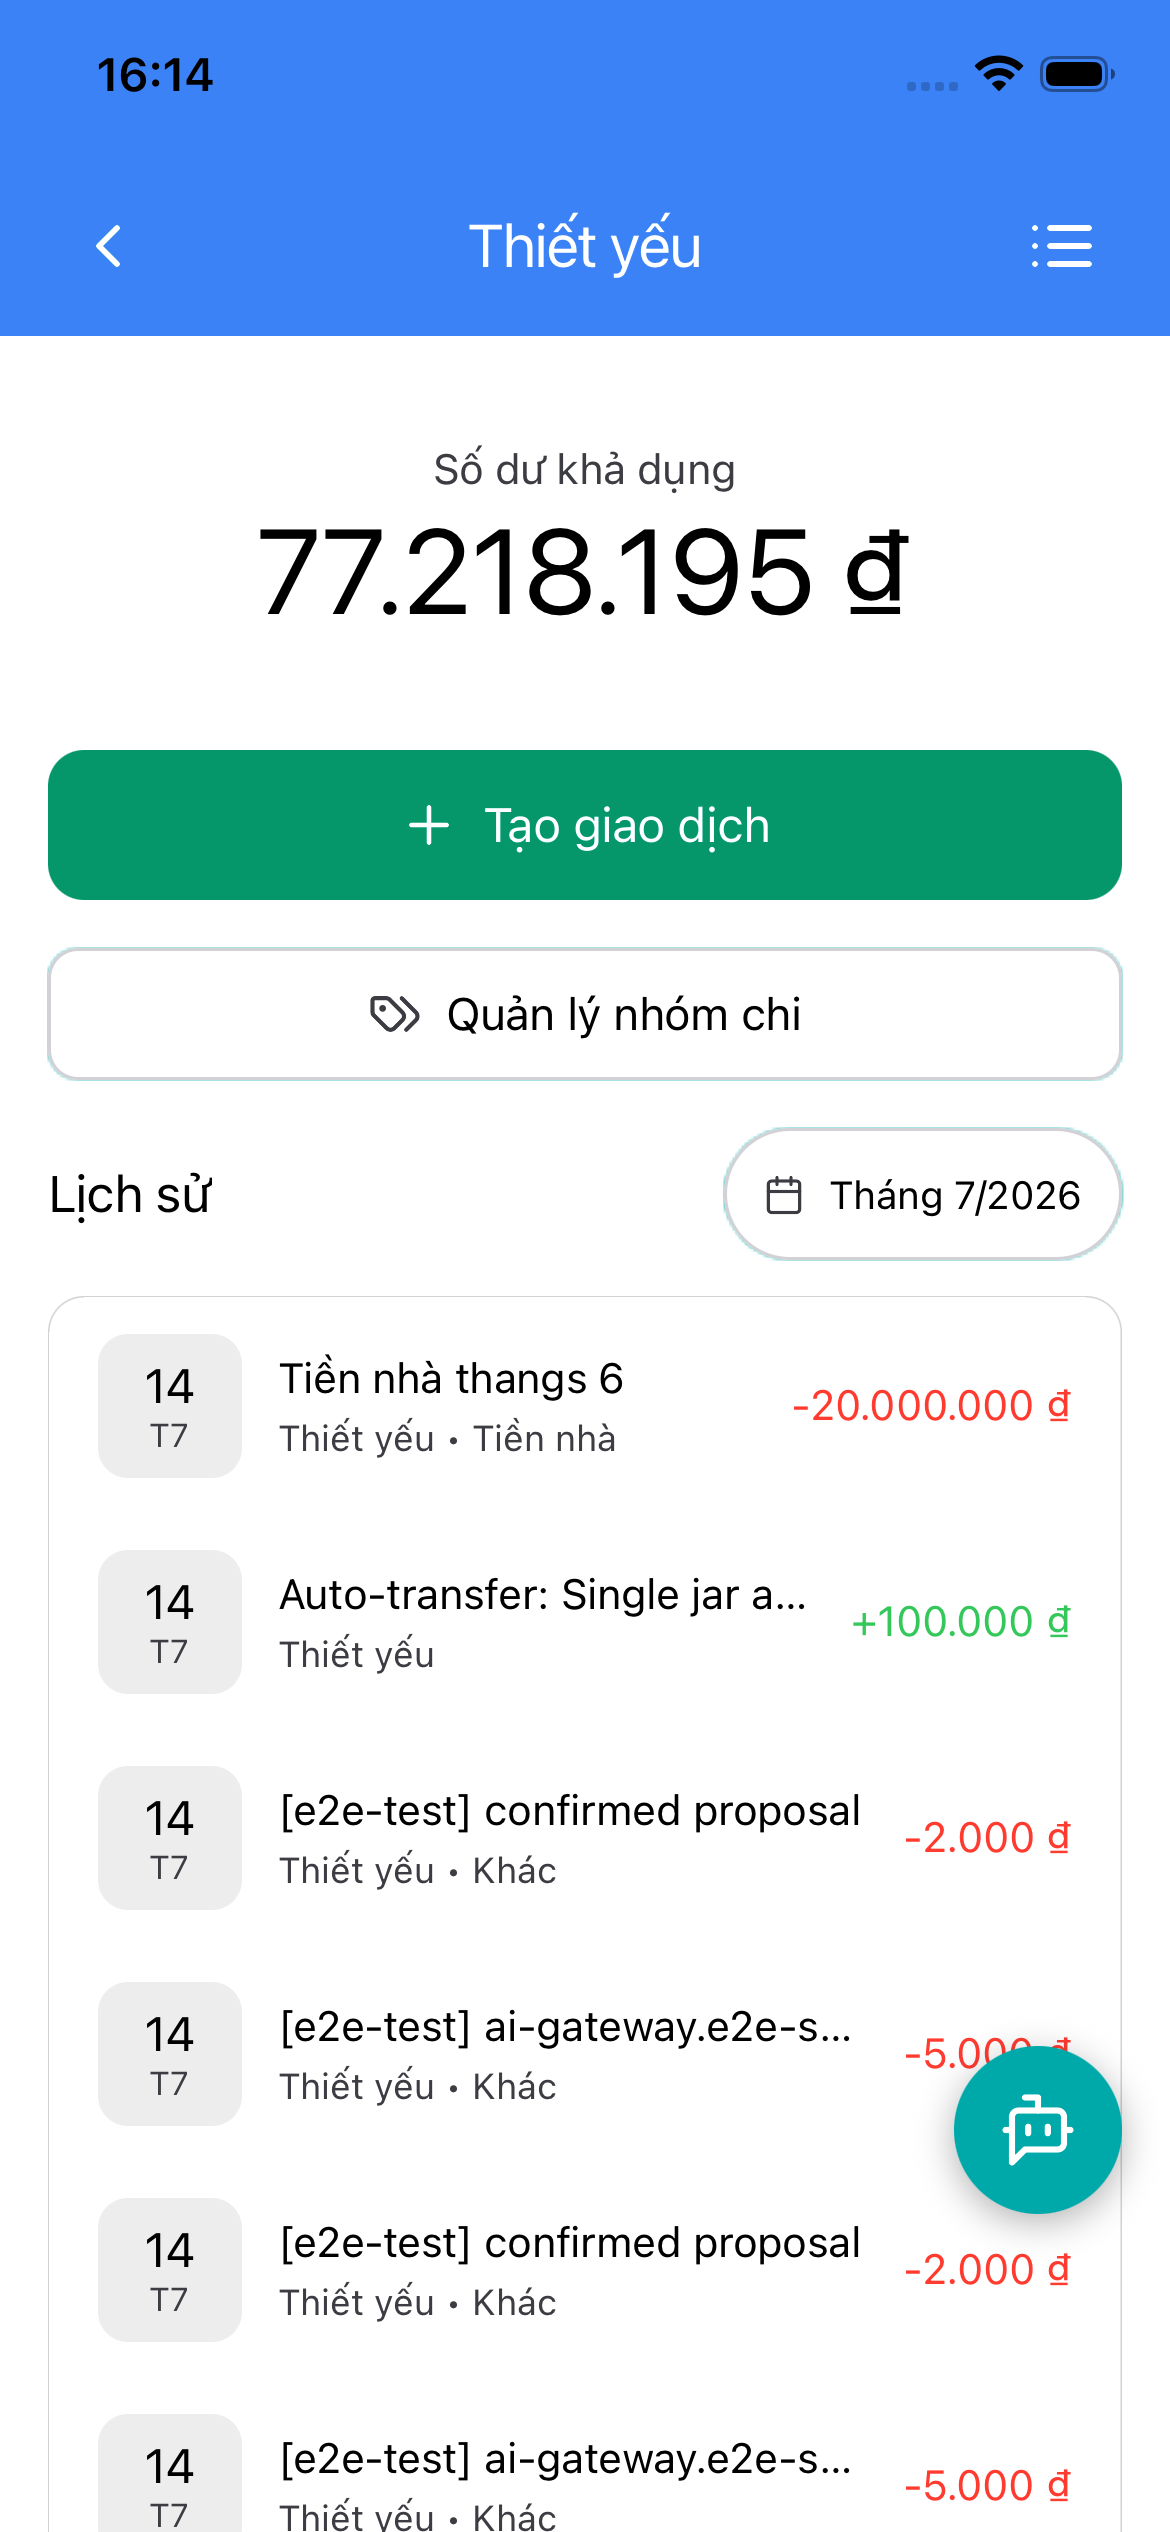
\includegraphics[width=0.4\textwidth]{images/chapter4/mobile/jar-detail.png}%
    }{%
        \rectbox{Hình ảnh màn hình chi tiết hũ trên Mobile}
    }
    \caption{Giao diện chi tiết hũ tài chính: số dư, ngưỡng cảnh báo và xu hướng dòng tiền}
    \label{fig:mobile-jar-detail}
\end{figure}

\begin{figure}[H]
    \noindent\textbf{3.} \textbf{Trò chuyện AI:} Màn hình này cho phép sinh viên trò chuyện trực tiếp với trợ lý tài chính ảo để truy vấn số dư hoặc thực hiện giao dịch nhanh bằng ngôn ngữ tự nhiên thông qua stream SSE thời gian thực. Giao diện cũng cung cấp một thanh menu sidebar để chuyển đổi nhanh các chủ đề. Sau khi AI Agent thực thi thành công một hành động tài chính (ví dụ: ghi nhận giao dịch mới qua lệnh tự nhiên), hệ thống áp dụng cơ chế Query Invalidation của React Query \cite{reactquery-docs} để tự động đánh dấu toàn bộ dữ liệu tài chính có liên quan là lỗi thời -- bao gồm số dư các hũ, lịch sử giao dịch và trang tổng quan -- rồi fetch lại ngầm và cập nhật UI tức thì mà không cần tải lại toàn bộ trang.
    
    \vspace{0.2cm}
    \centering
    \begin{minipage}{0.44\textwidth}
        \centering
        \IfFileExists{images/chapter4/mobile/ai-chat.png}{%
            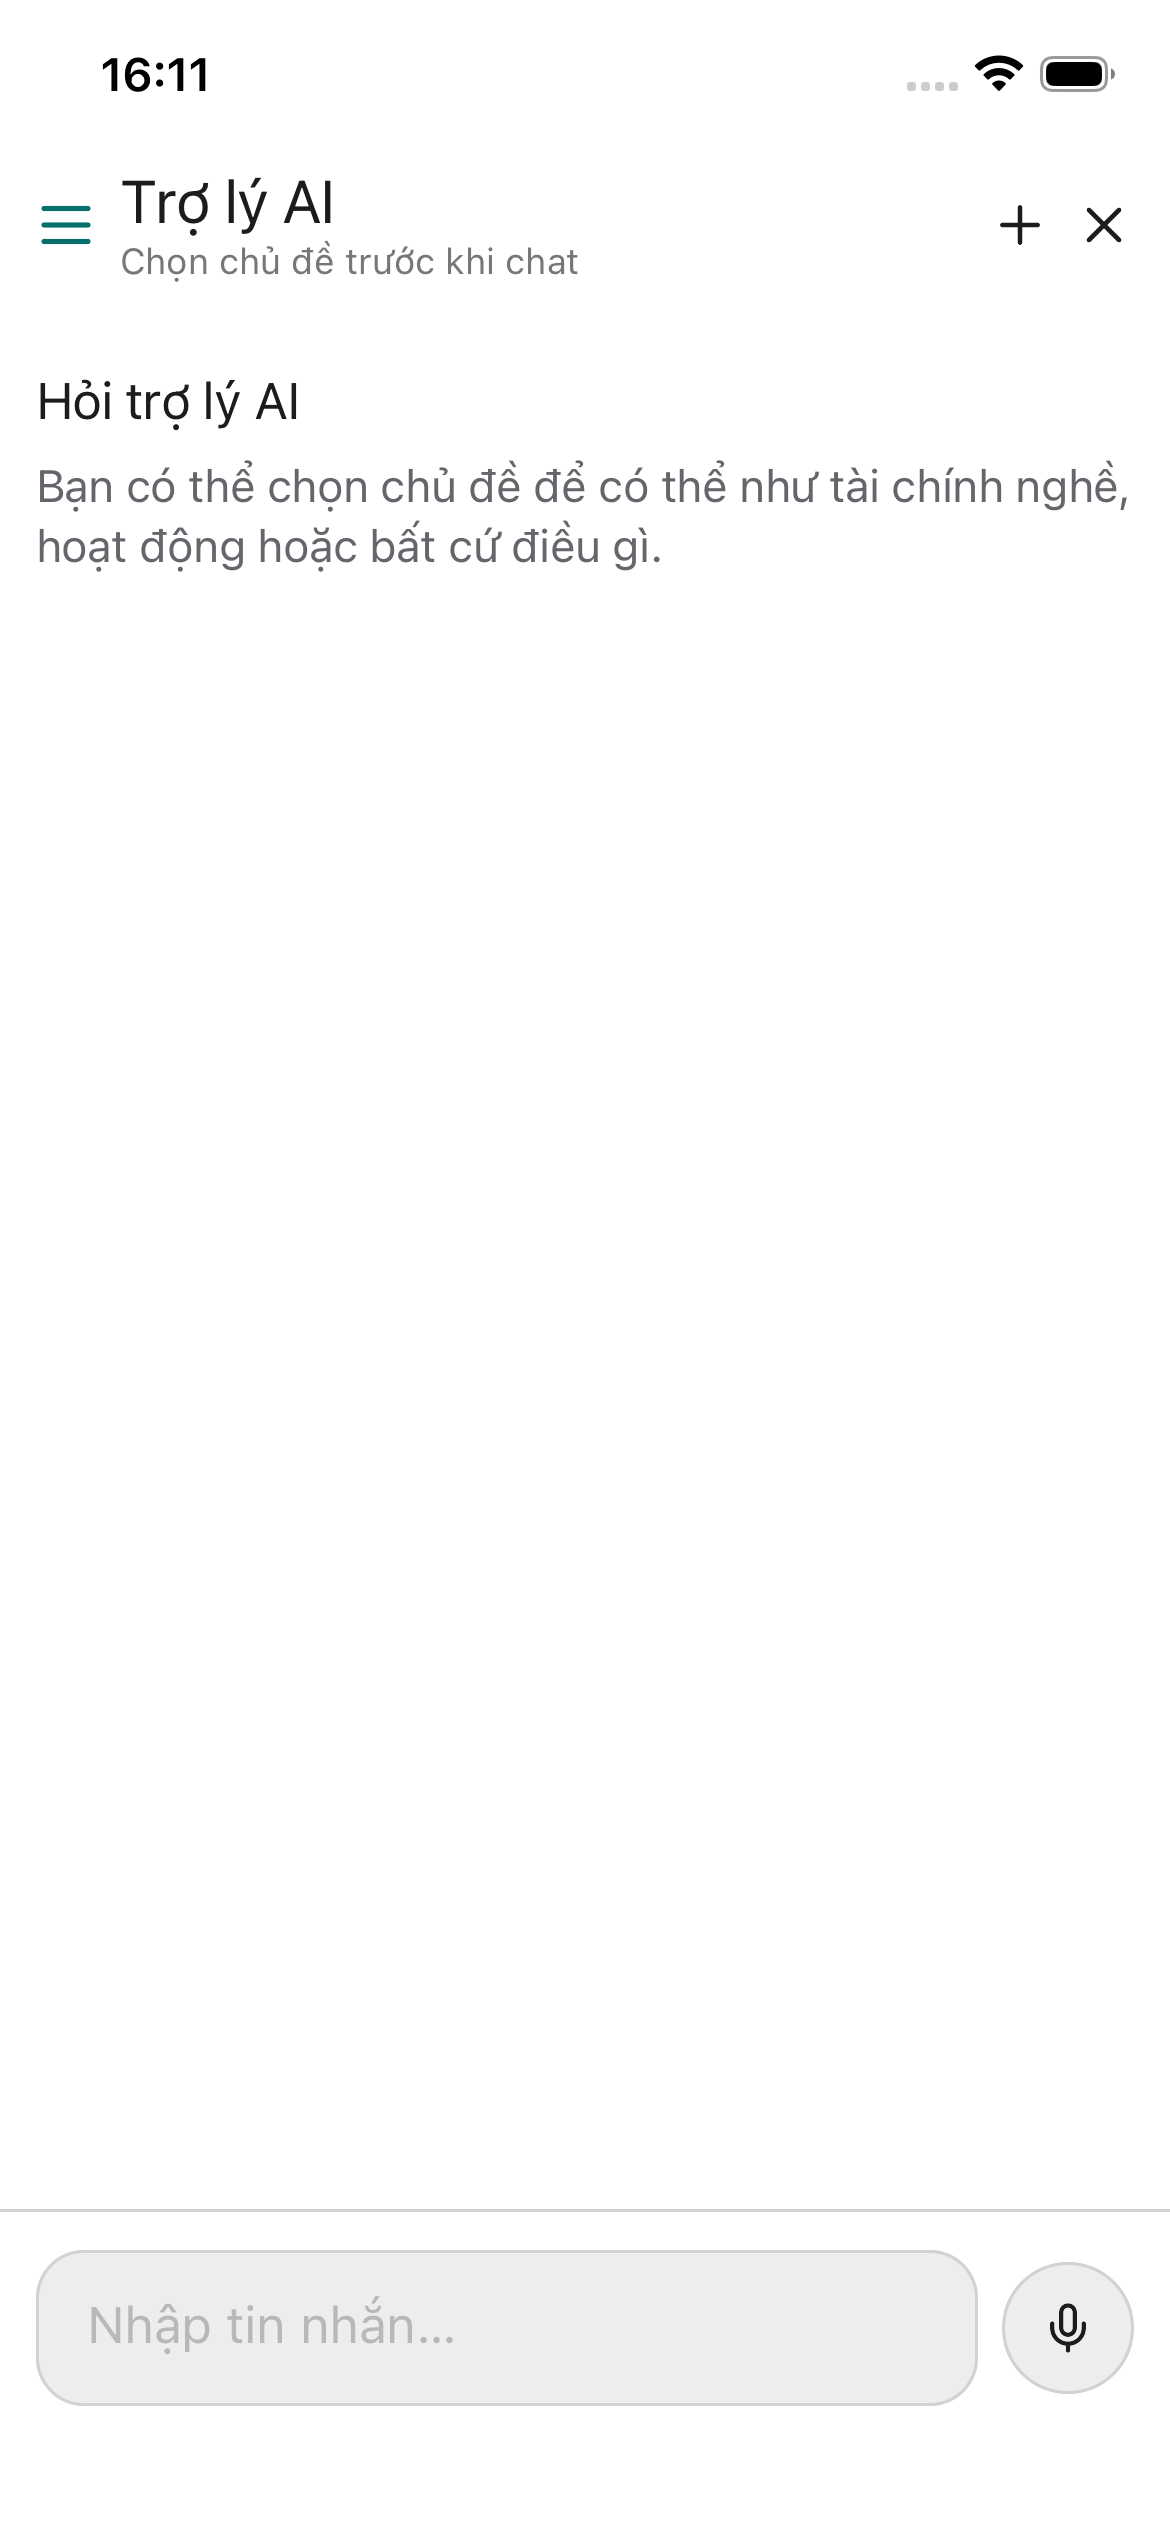
\includegraphics[width=\textwidth]{images/chapter4/mobile/ai-chat.png}%
        }{%
            \rectbox{Hình ảnh màn hình Chat AI Trợ lý}
        }
        \caption{Giao diện trò chuyện thời gian thực với trợ lý AI}
        \label{fig:mobile-aichat}
    \end{minipage}
    \hfill
    \begin{minipage}{0.44\textwidth}
        \centering
        \IfFileExists{images/chapter4/mobile/ai-chat-sidebar.png}{%
            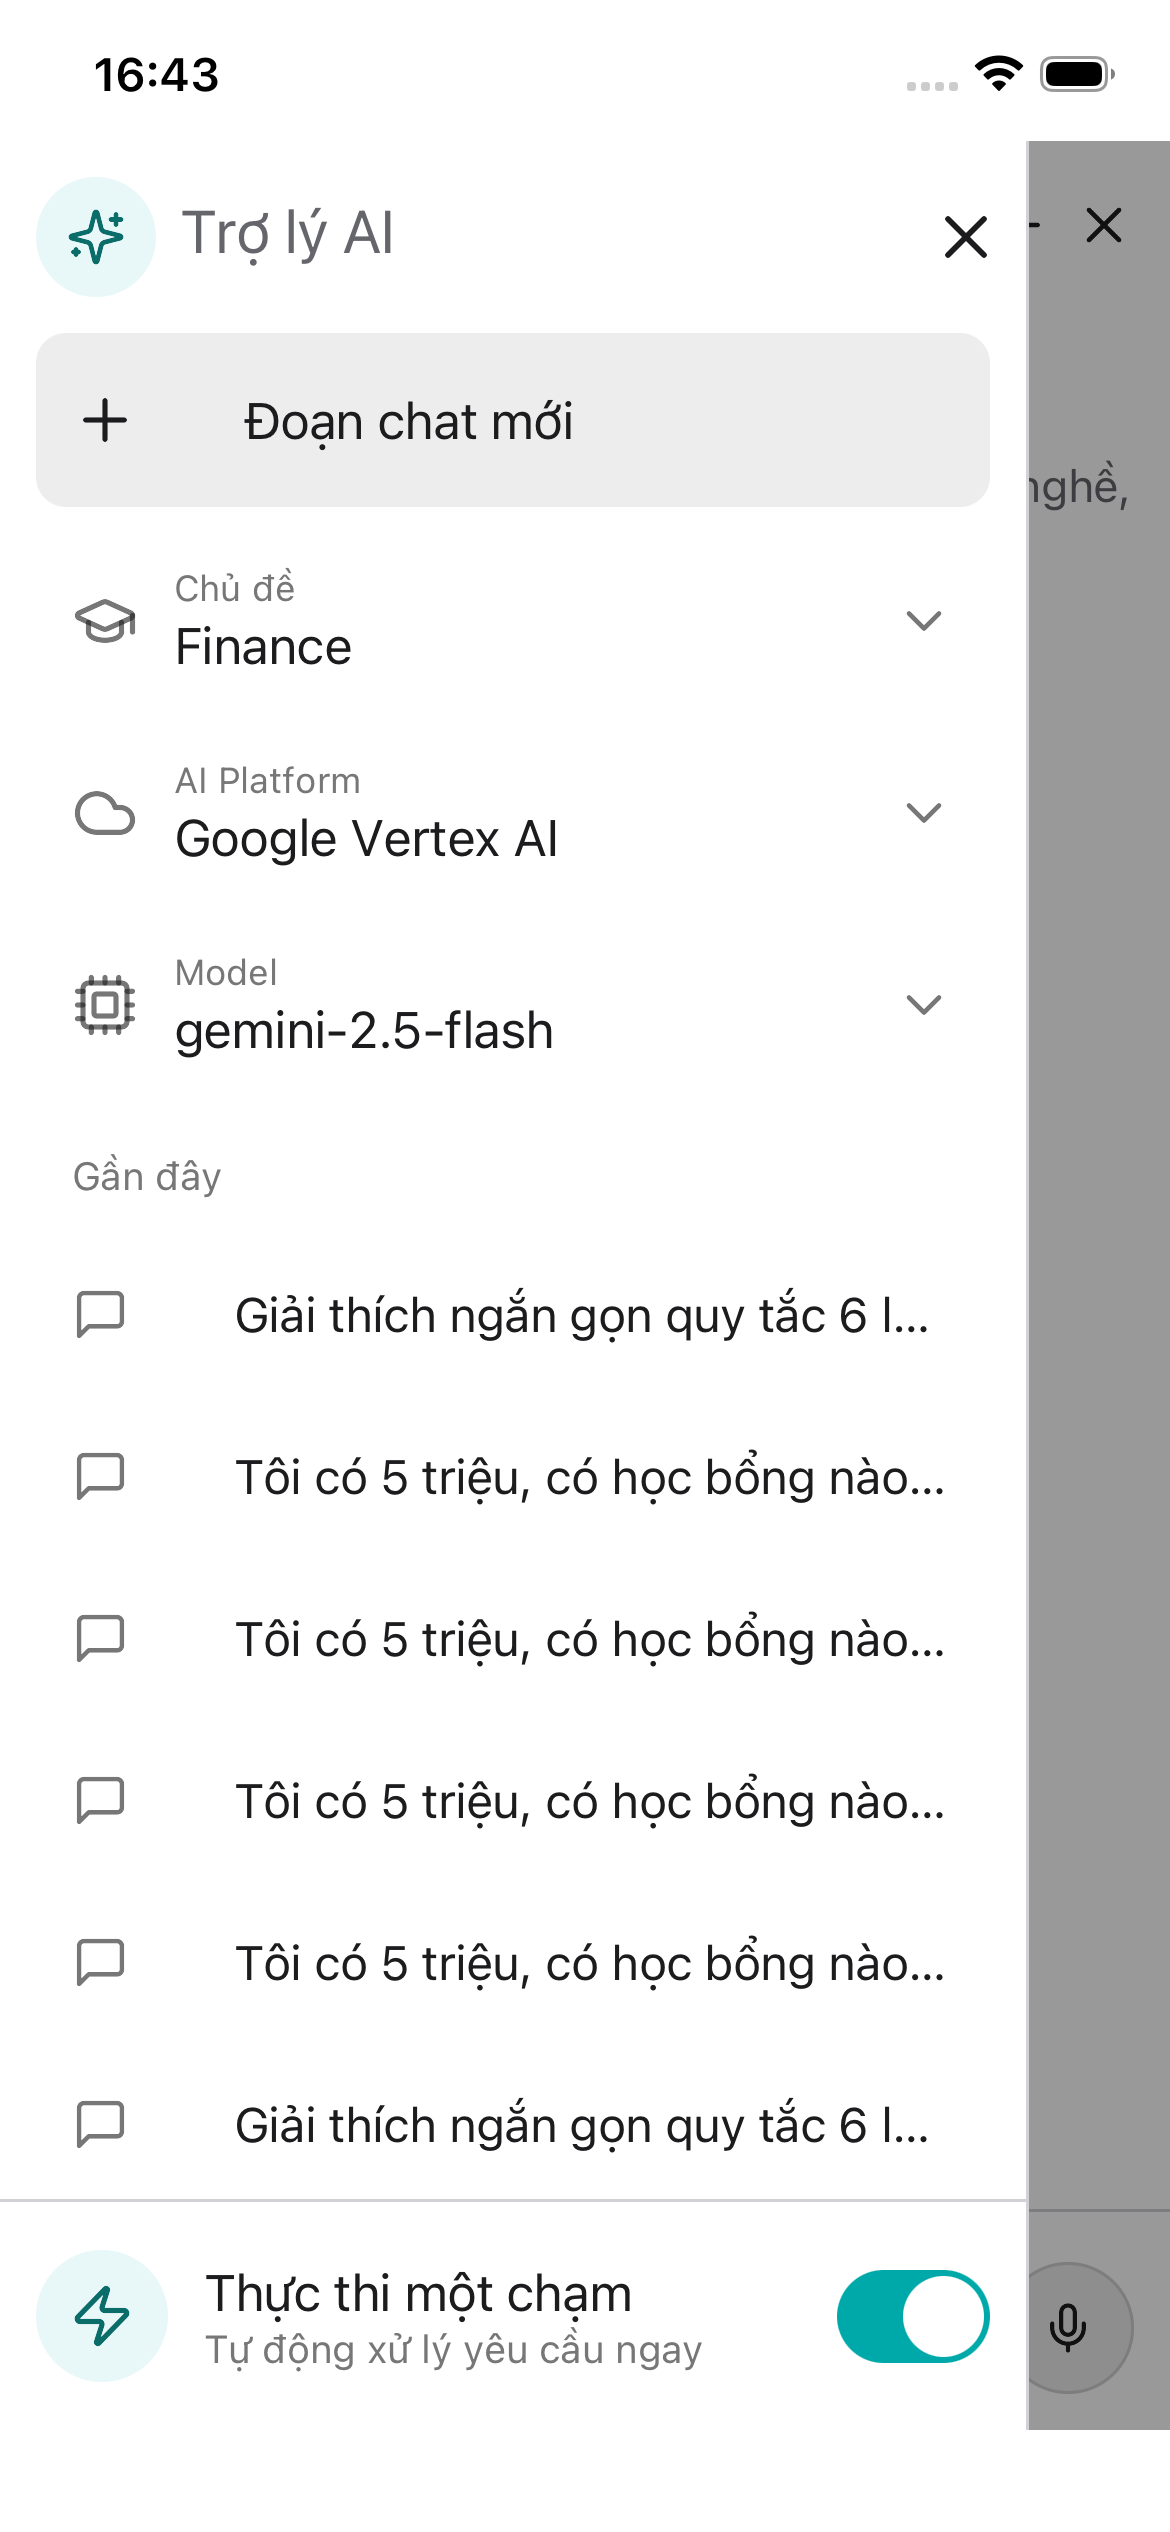
\includegraphics[width=\textwidth]{images/chapter4/mobile/ai-chat-sidebar.png}%
        }{%
            \rectbox{Hình ảnh bảng chọn chủ đề và mô hình AI}
        }
        \caption{Bảng chọn chủ đề, nền tảng AI và lịch sử trò chuyện gần đây}
        \label{fig:mobile-aichat-sidebar}
    \end{minipage}
\end{figure}

\begin{figure}[H]
    \noindent\textbf{4.} \textbf{Cấu hình phân bổ lọ:} Màn hình này hỗ trợ sinh viên kéo thả thanh trượt để thay đổi phần trăm phân bổ thu nhập tự động vào 6 hũ tài chính. Hệ thống ràng buộc tổng tỷ lệ luôn đạt chính xác 100\% trước khi lưu cấu hình mới.
    
    \vspace{0.2cm}
    \centering
    \IfFileExists{images/chapter4/mobile/jar-allocation.png}{%
        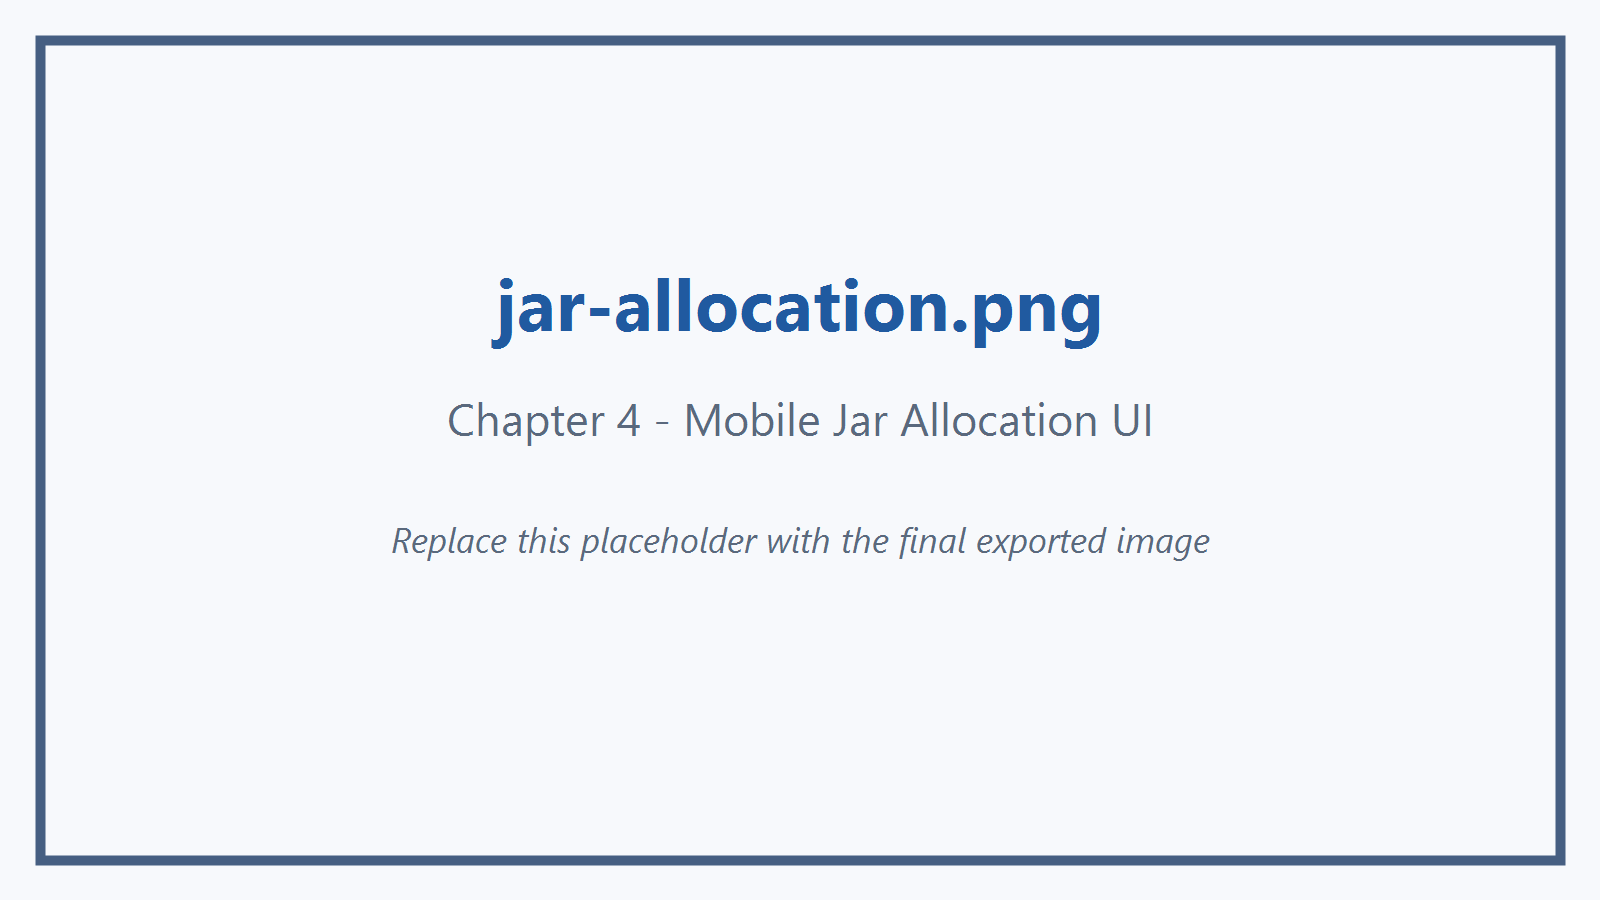
\includegraphics[width=0.4\textwidth]{images/chapter4/mobile/jar-allocation.png}%
    }{%
        \rectbox{Hình ảnh màn hình điều chỉnh tỷ lệ 6 lọ trên Mobile}
    }
    \caption{Giao diện cấu hình phần trăm phân bổ hũ tài chính (tổng luôn bằng 100\%)}
    \label{fig:mobile-jar-alloc}
\end{figure}
\clearpage

\begin{figure}[H]
    \noindent\textbf{5.} \textbf{Ghi chép giao dịch:} Màn hình này cung cấp biểu mẫu nhập giao dịch thu chi mới. Đối với các giao dịch thu nhập, hệ thống tự động hiển thị modal phân bổ nhanh vào các hũ theo tỷ lệ định cấu hình trước đó để chia tiền tự động. Ngay sau khi giao dịch được lưu thành công, mutation hook của React Query \cite{reactquery-docs} lập tức invalidate toàn bộ cache tài chính liên quan (số dư hũ, lịch sử, biểu đồ báo cáo), đảm bảo dữ liệu hiển thị luôn phản ánh chính xác trạng thái mới nhất mà không cần sinh viên phải tải lại ứng dụng.
    
    \vspace{0.2cm}
    \centering
    \begin{minipage}{0.44\textwidth}
        \centering
        \IfFileExists{images/chapter4/mobile/add-transaction.png}{%
            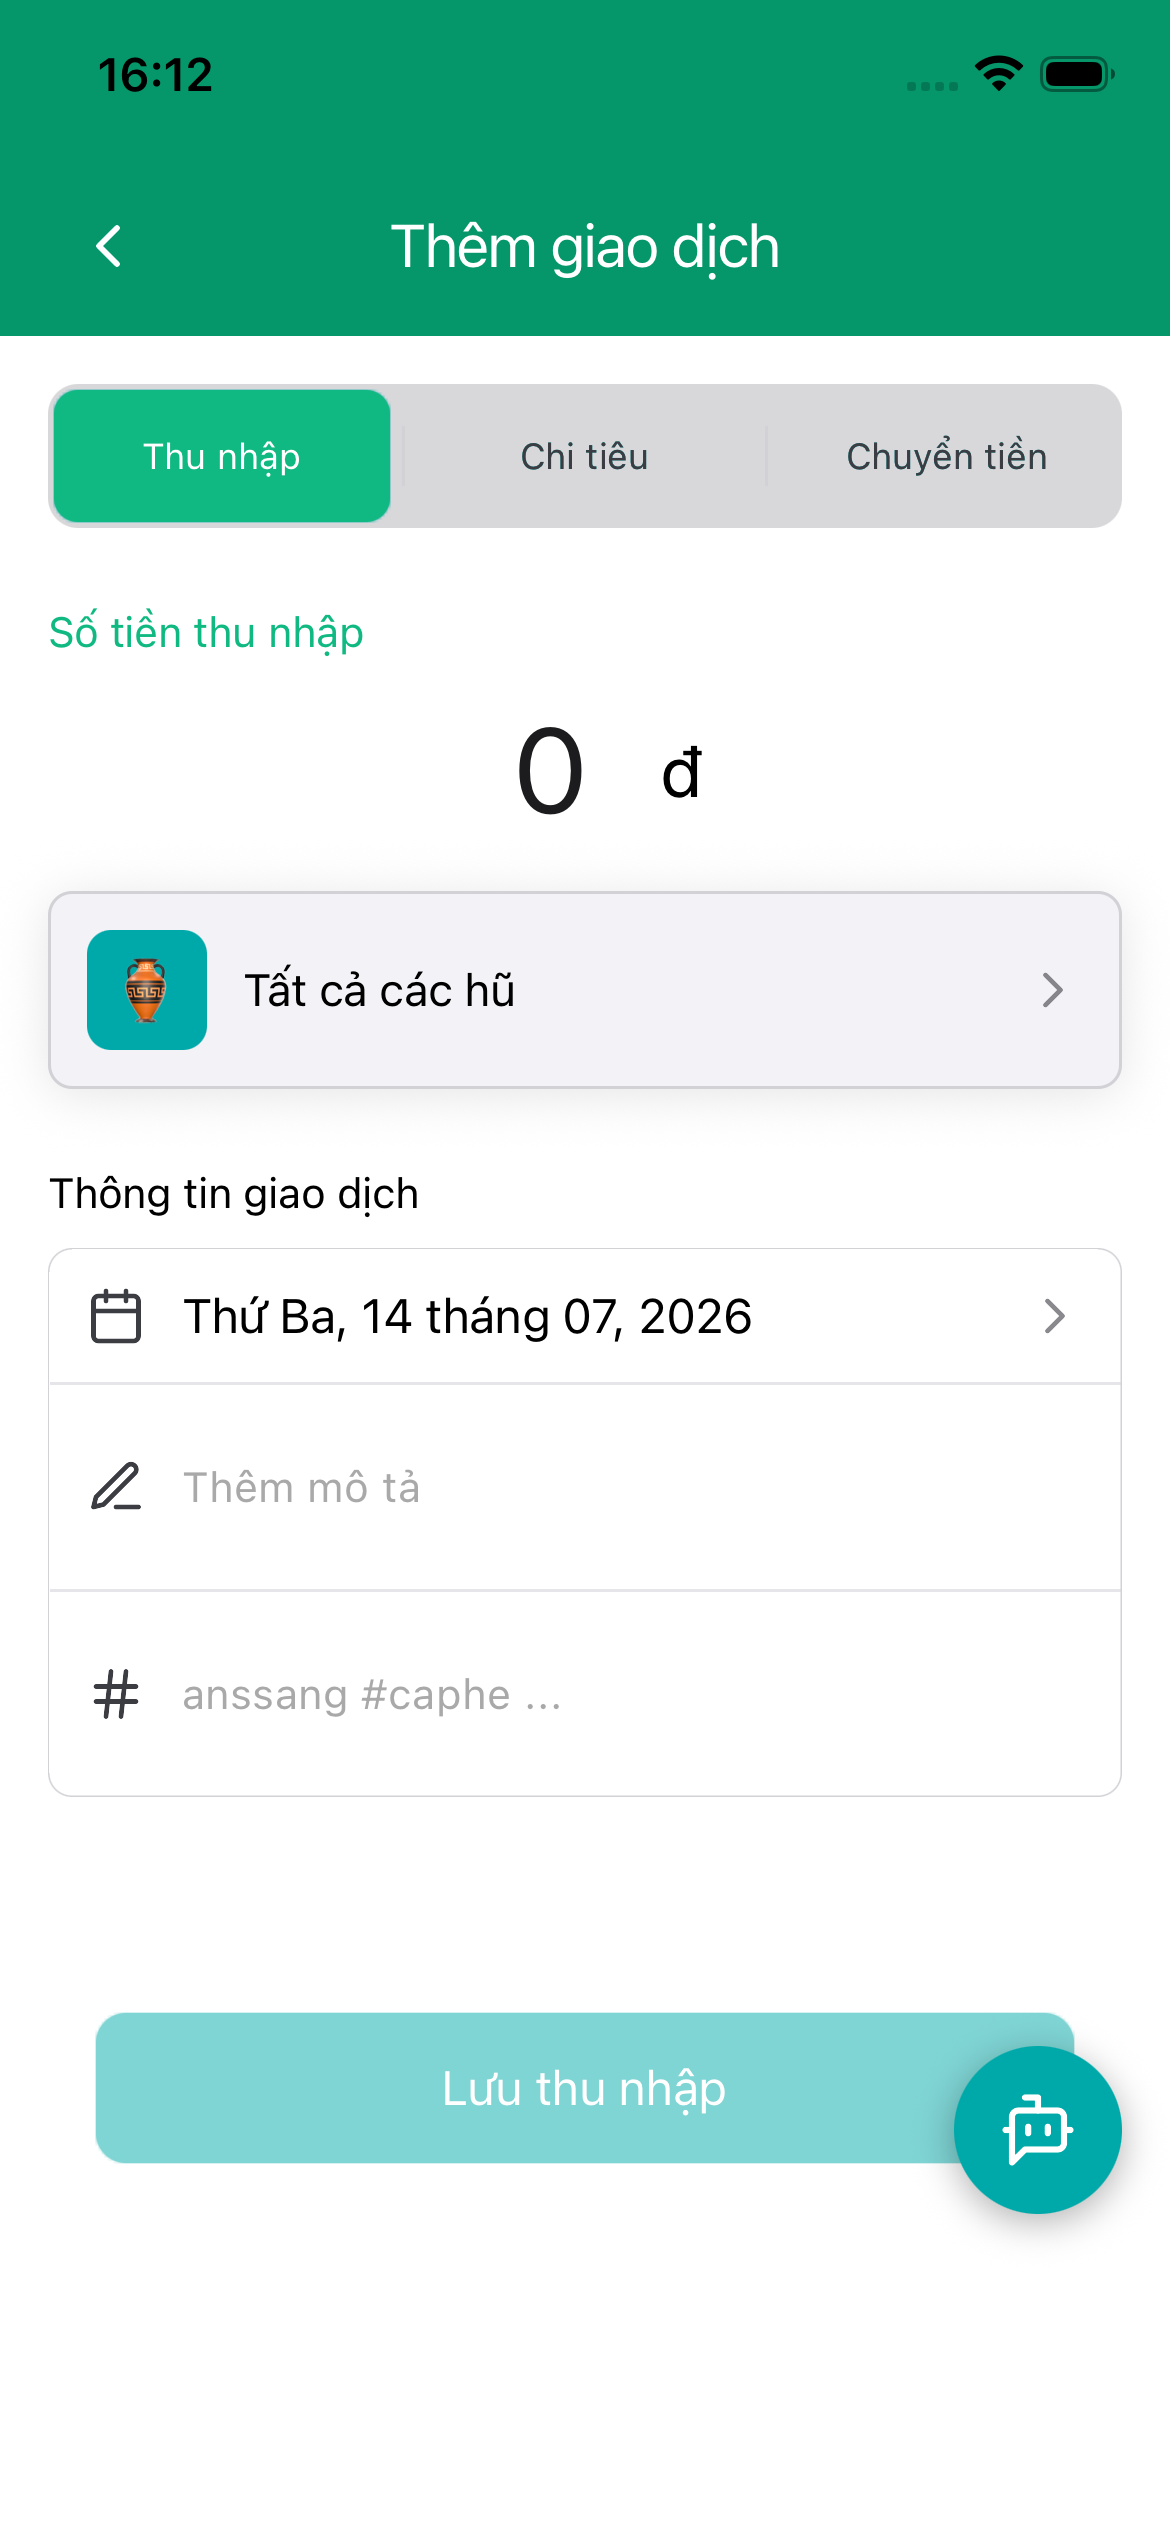
\includegraphics[width=\textwidth]{images/chapter4/mobile/add-transaction.png}%
        }{%
            \rectbox{Hình ảnh màn hình thêm mới giao dịch trên Mobile}
        }
        \caption{Giao diện biểu mẫu thêm mới giao dịch tài chính}
        \label{fig:mobile-add-transaction}
    \end{minipage}
    \hfill
    \begin{minipage}{0.44\textwidth}
        \centering
        \IfFileExists{images/chapter4/mobile/add-transaction-allocation.png}{%
            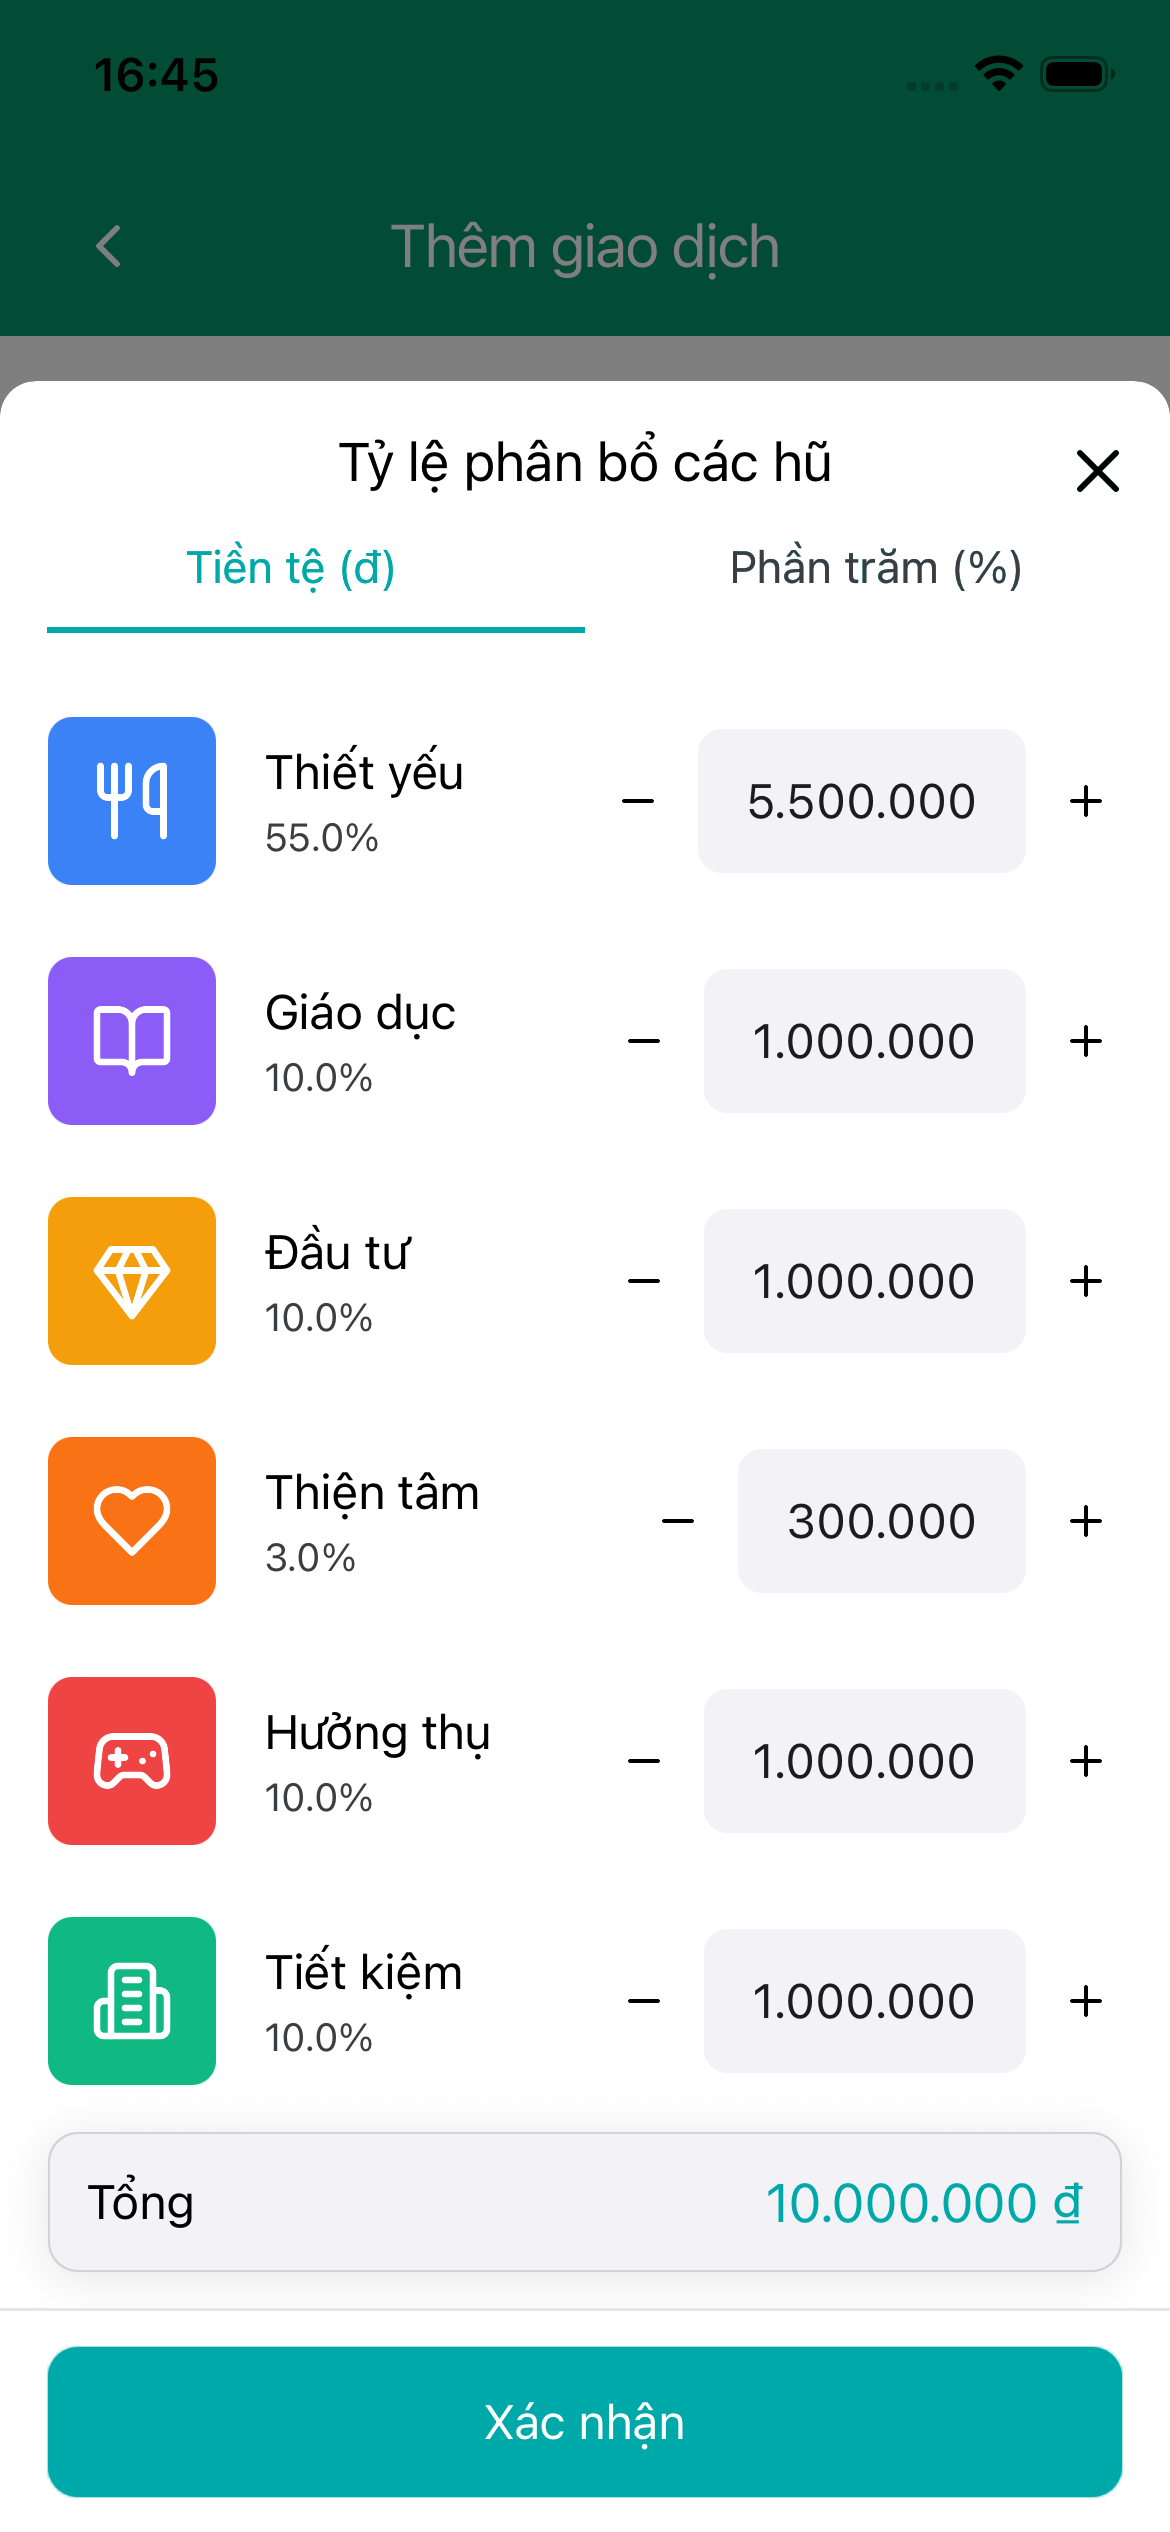
\includegraphics[width=\textwidth]{images/chapter4/mobile/add-transaction-allocation.png}%
        }{%
            \rectbox{Hình ảnh modal thiết lập tỷ lệ phân bổ khi thêm thu nhập}
        }
        \caption{Modal thiết lập tỷ lệ phân bổ vào các hũ khi ghi nhận thu nhập}
        \label{fig:mobile-add-transaction-allocation}
    \end{minipage}
\end{figure}

\begin{figure}[H]
    \noindent\textbf{6.} \textbf{Lịch sử giao dịch:} Màn hình này liệt kê chi tiết các giao dịch thu chi đã được ghi nhận trong hệ thống. Sinh viên có thể tra cứu nhanh theo nội dung giao dịch hoặc lọc giao dịch theo hũ cụ thể và mốc thời gian.
    
    \vspace{0.2cm}
    \centering
    \IfFileExists{images/chapter4/mobile/transaction-history.png}{%
        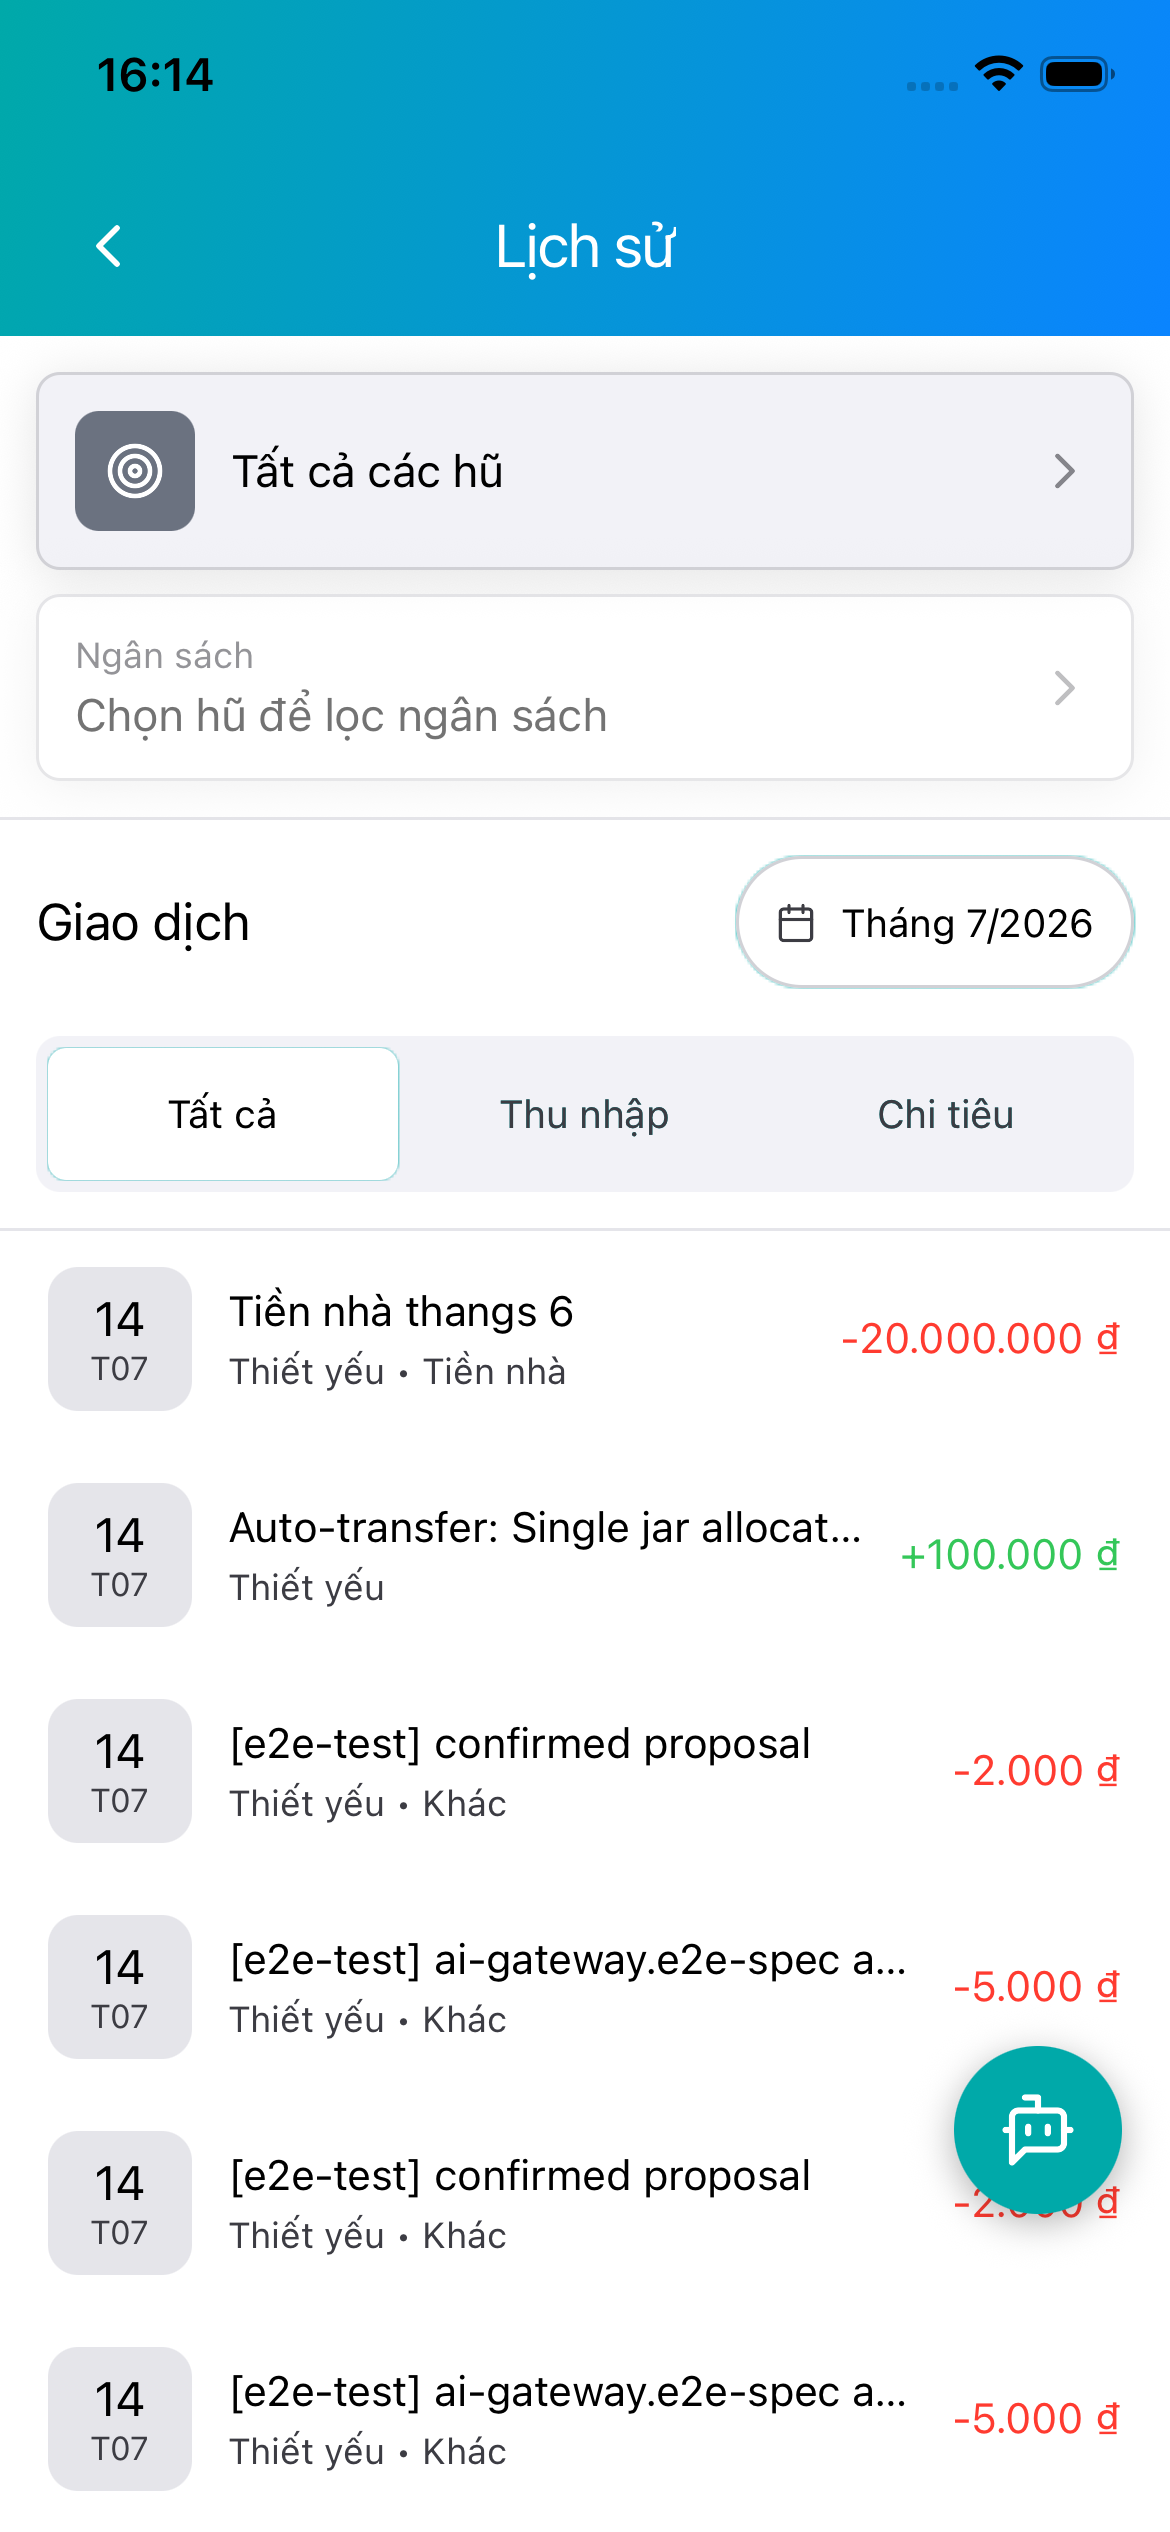
\includegraphics[width=0.4\textwidth]{images/chapter4/mobile/transaction-history.png}%
    }{%
        \rectbox{Hình ảnh danh sách lịch sử giao dịch trên Mobile}
    }
    \caption{Giao diện danh sách lịch sử giao dịch, hỗ trợ tìm kiếm và lọc theo hũ/thời gian}
    \label{fig:mobile-transaction-history}
\end{figure}
\clearpage

\begin{figure}[H]
    \noindent\textbf{7.} \textbf{Lịch chuyển tiền tự động:} Màn hình này cho phép thiết lập và quản lý các giao dịch chuyển tiền tự động định kỳ giữa các hũ tài chính. Người dùng có thể chỉnh sửa số tiền, chu kỳ lặp lại và trạng thái kích hoạt của lịch chuyển.
    
    \vspace{0.2cm}
    \centering
    \begin{minipage}{0.44\textwidth}
        \centering
        \IfFileExists{images/chapter4/mobile/auto-transfer.png}{%
            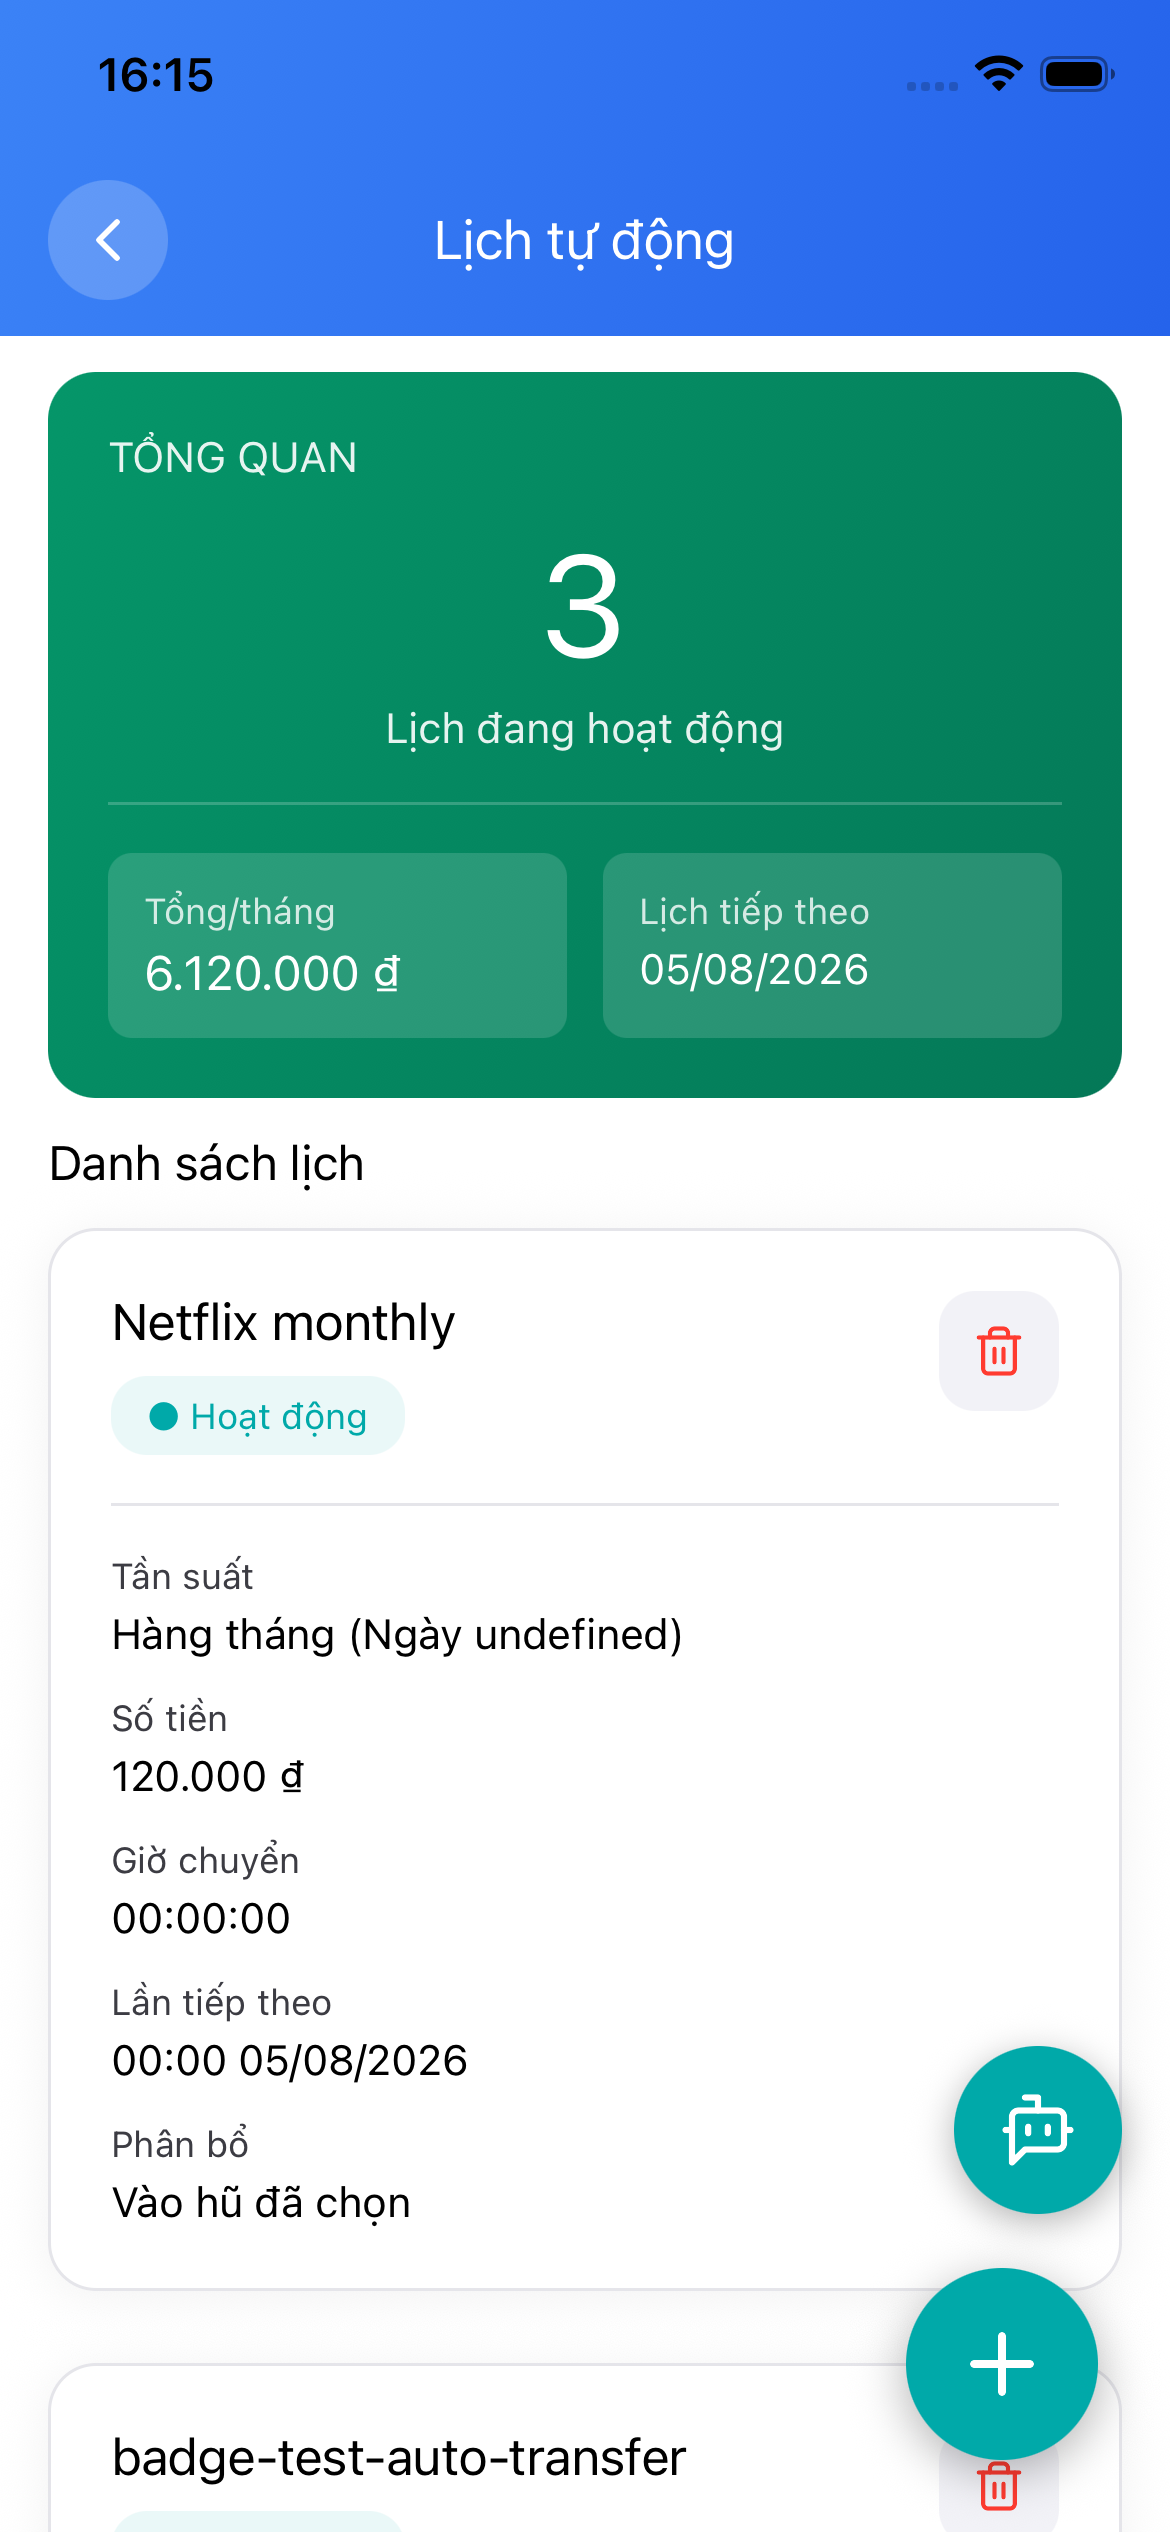
\includegraphics[width=\textwidth]{images/chapter4/mobile/auto-transfer.png}%
        }{%
            \rectbox{Hình ảnh màn hình quản lý lịch chuyển tự động trên Mobile}
        }
        \caption{Giao diện quản lý lịch chuyển tiền tự động}
        \label{fig:mobile-auto-transfer}
    \end{minipage}
    \hfill
    \begin{minipage}{0.44\textwidth}
        \centering
        \IfFileExists{images/chapter4/mobile/auto-transfer-edit.png}{%
            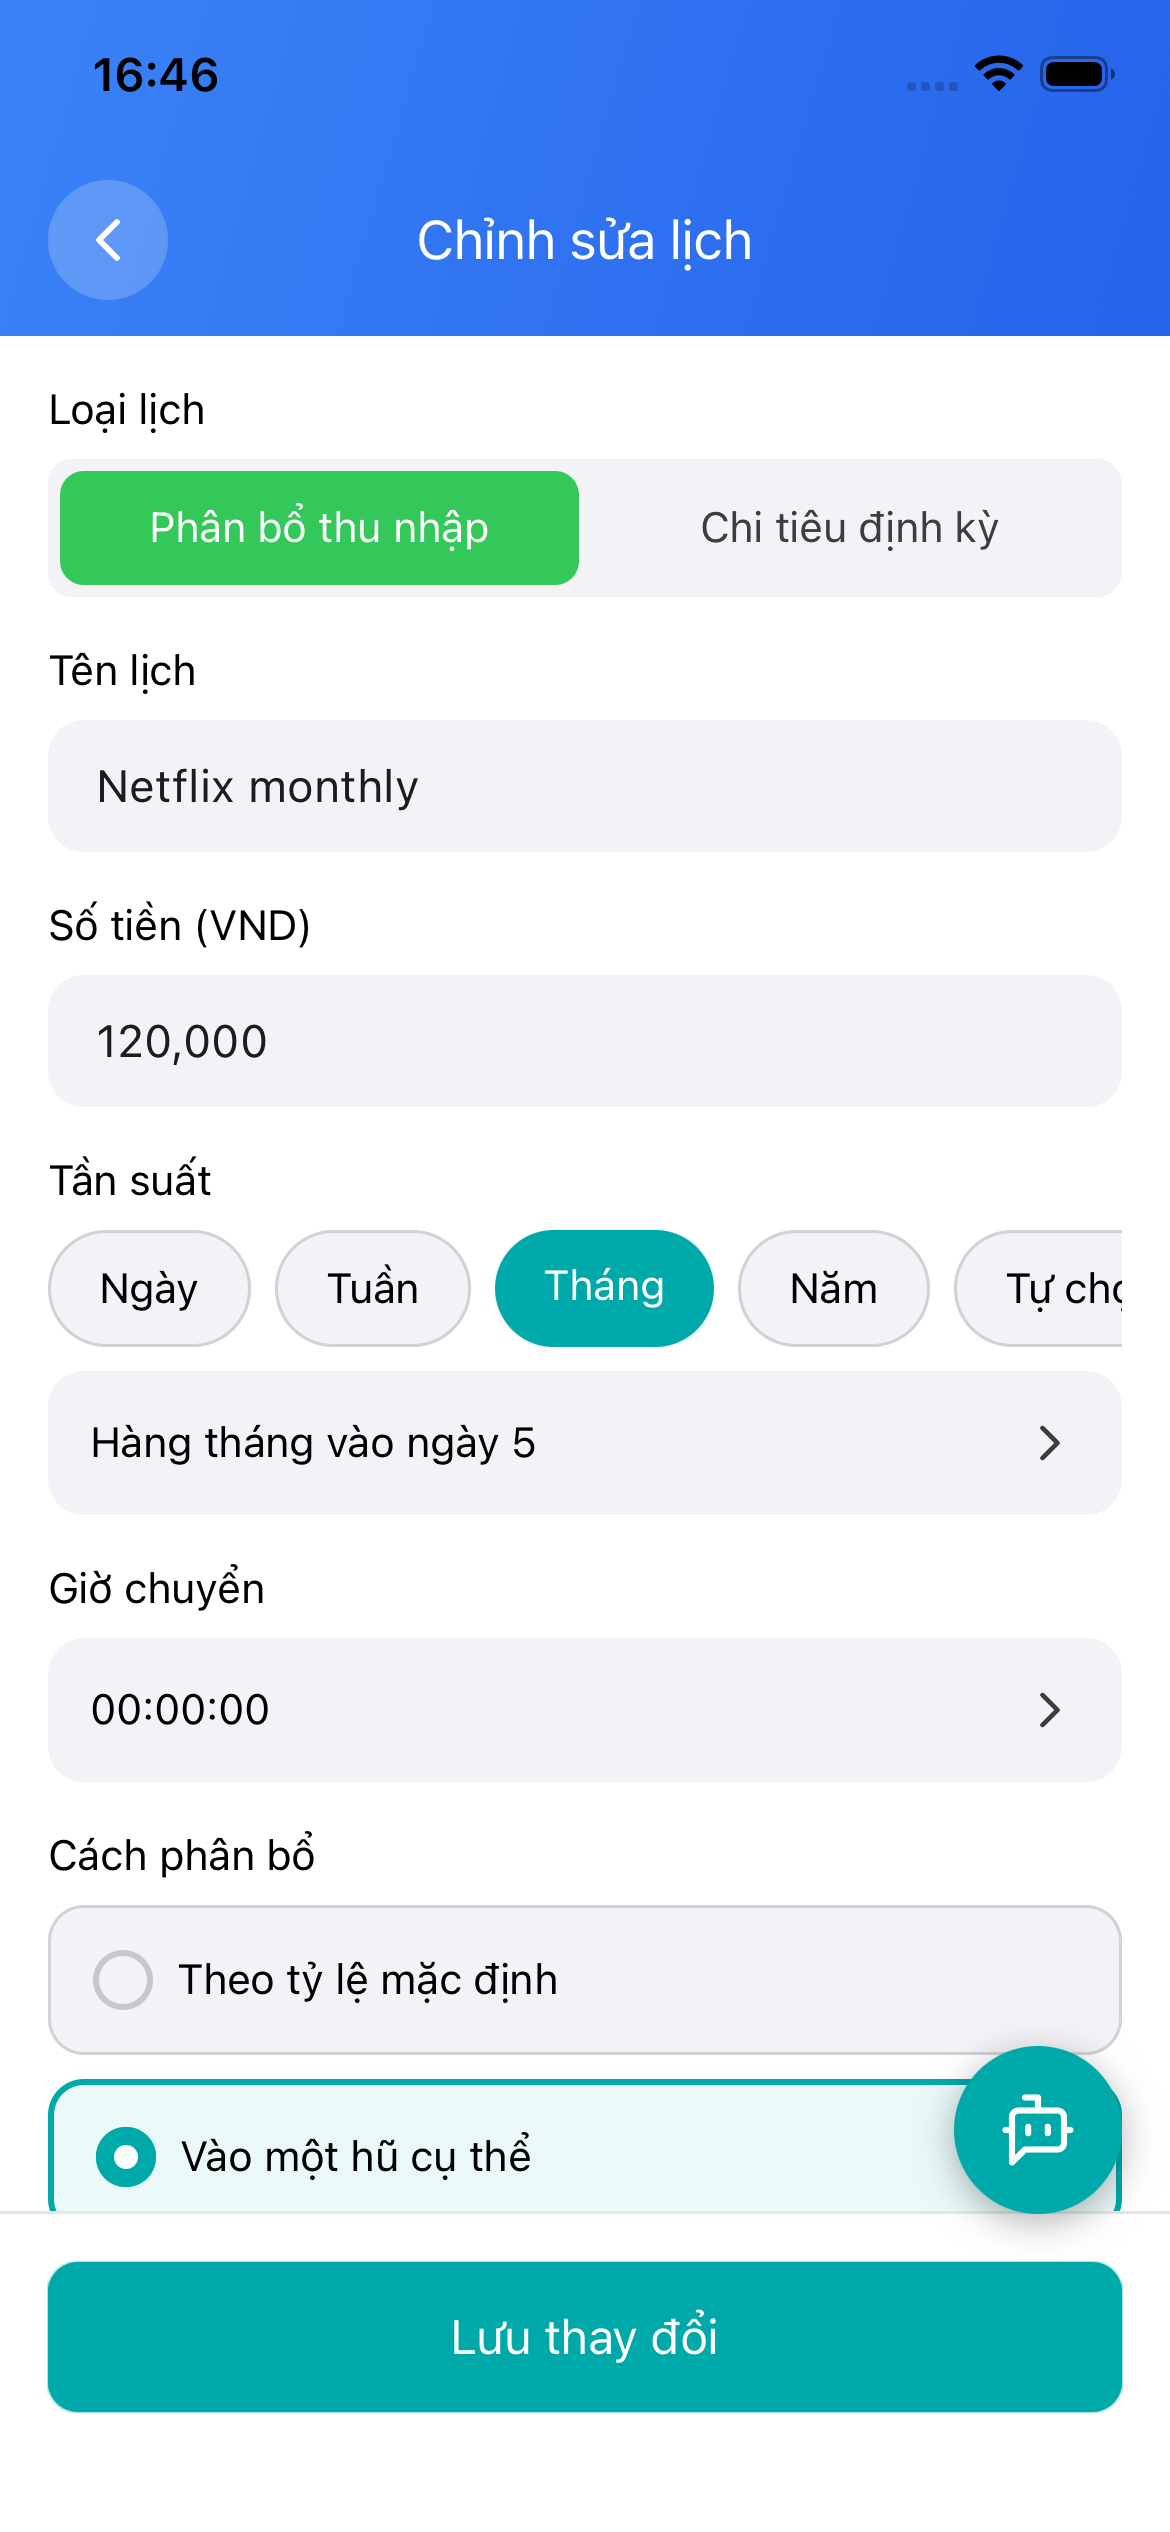
\includegraphics[width=\textwidth]{images/chapter4/mobile/auto-transfer-edit.png}%
        }{%
            \rectbox{Hình ảnh biểu mẫu chỉnh sửa lịch chuyển tiền tự động}
        }
        \caption{Biểu mẫu chỉnh sửa lịch chuyển tiền tự động}
        \label{fig:mobile-auto-transfer-edit}
    \end{minipage}
\end{figure}

\begin{figure}[H]
    \noindent\textbf{8.} \textbf{Báo cáo tài chính:} Màn hình này hiển thị biểu đồ thống kê các khoản thu chi định kỳ và phân bổ dòng tiền. Tại đây tích hợp mô-đun AI Insights tự động nhận định thói quen tiêu dùng của sinh viên và gửi các khuyến nghị tối ưu tài chính.
    
    \vspace{0.2cm}
    \centering
    \begin{minipage}{0.44\textwidth}
        \centering
        \IfFileExists{images/chapter4/mobile/financial-report.png}{%
            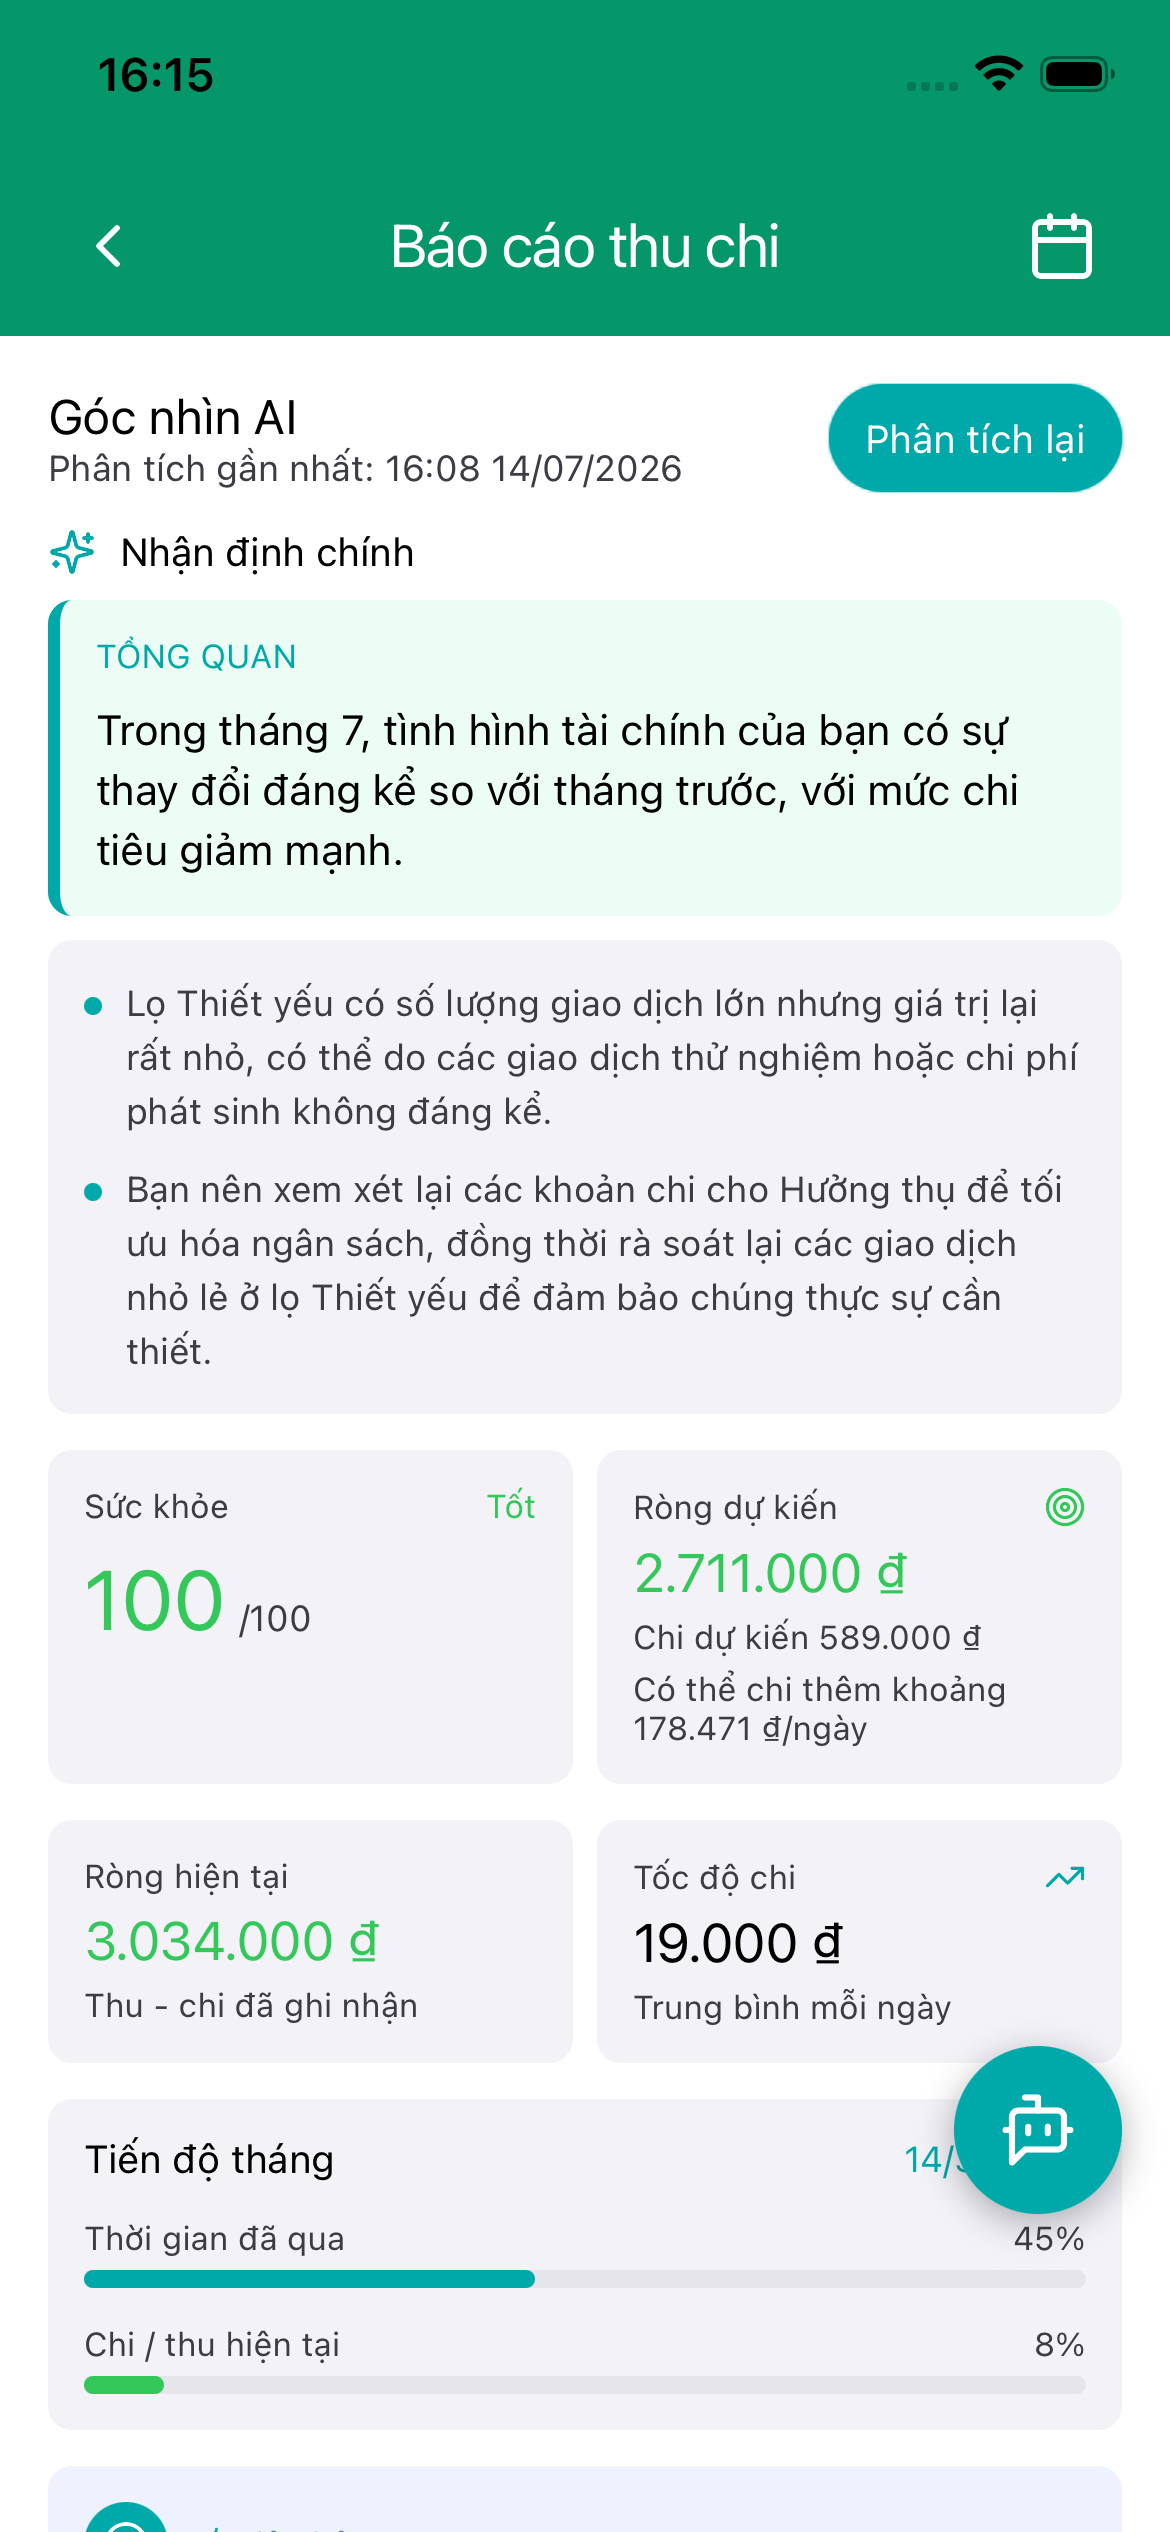
\includegraphics[width=\textwidth]{images/chapter4/mobile/financial-report.png}%
        }{%
            \rectbox{Hình ảnh màn hình báo cáo phân tích tài chính trên Mobile}
        }
        \caption{Giao diện báo cáo phân tích tài chính chi tiêu}
        \label{fig:mobile-financial-report}
    \end{minipage}
    \hfill
    \begin{minipage}{0.44\textwidth}
        \centering
        \IfFileExists{images/chapter4/mobile/financial-report-chart.png}{%
            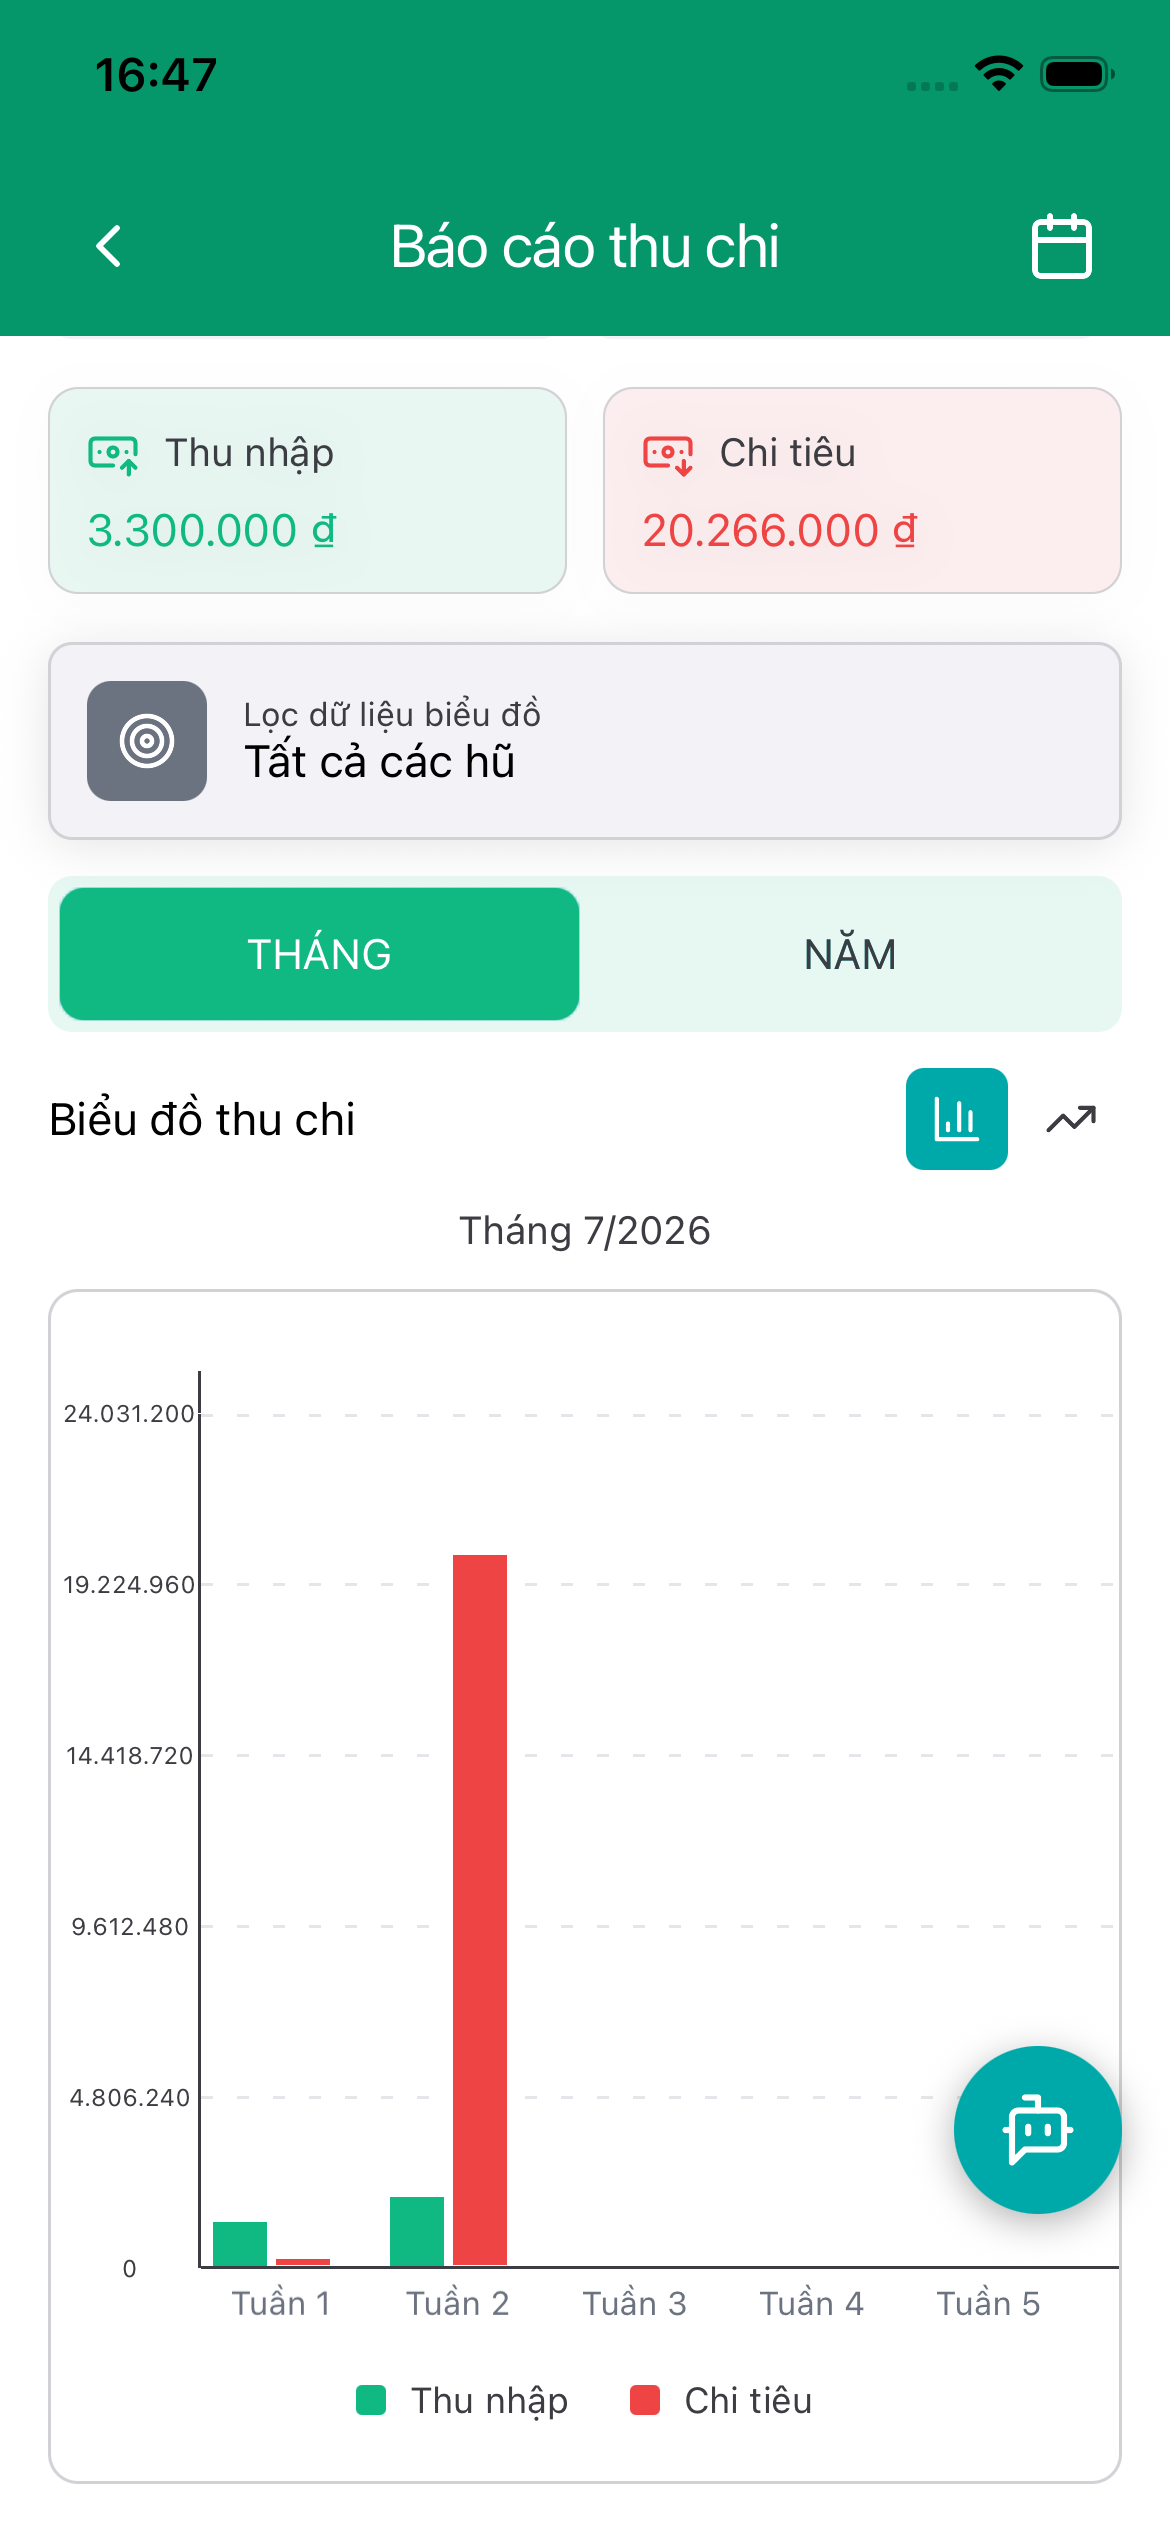
\includegraphics[width=\textwidth]{images/chapter4/mobile/financial-report-chart.png}%
        }{%
            \rectbox{Hình ảnh biểu đồ thu chi theo tuần trên báo cáo tài chính}
        }
        \caption{Biểu đồ thu chi theo tuần và AI Insights trên màn hình báo cáo}
        \label{fig:mobile-financial-report-chart}
    \end{minipage}
\end{figure}
\clearpage

\begin{figure}[H]
    \noindent\textbf{9.} \textbf{Gợi ý học bổng:} Màn hình này hiển thị danh sách các học bổng trực tuyến phù hợp nhất với sinh viên, được sắp xếp tự động dựa trên điểm tương thích hồ sơ (GPA, ngành học) của từng sinh viên.
    
    \vspace{0.2cm}
    \centering
    \begin{minipage}{0.44\textwidth}
        \centering
        \IfFileExists{images/chapter4/mobile/H5.14-1.png}{%
            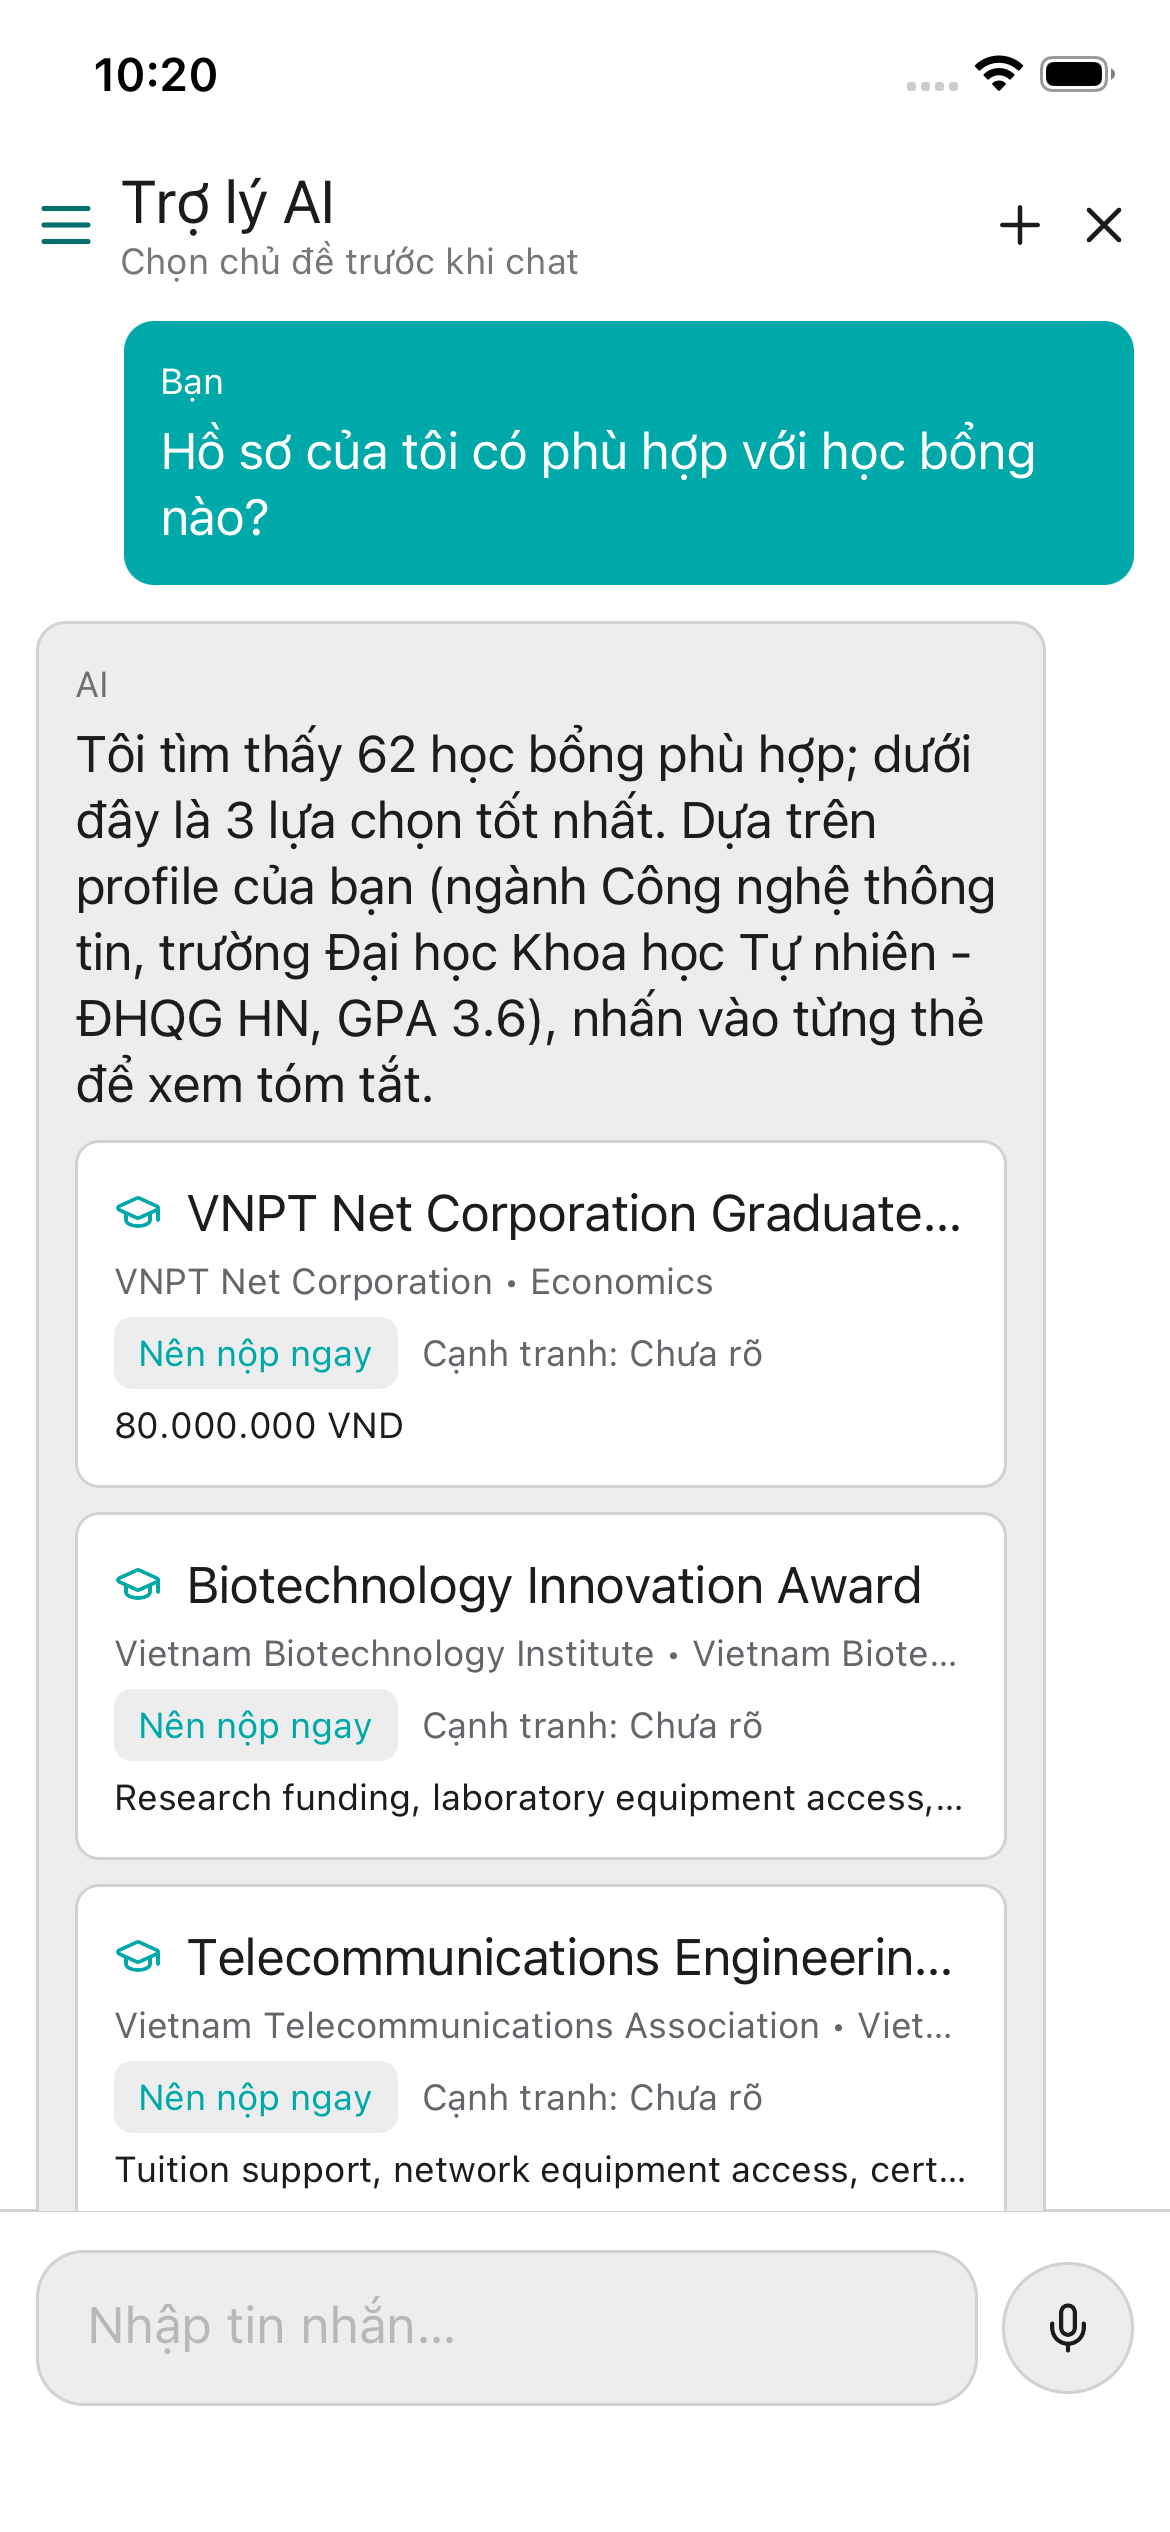
\includegraphics[width=\textwidth]{images/chapter4/mobile/H5.14-1.png}%
        }{%
            \rectbox{Gợi ý học bổng 1}
        }
        \centerline{(a) Danh sách gợi ý học bổng}
    \end{minipage}
    \hfill
    \begin{minipage}{0.44\textwidth}
        \centering
        \IfFileExists{images/chapter4/mobile/H5.14-2.png}{%
            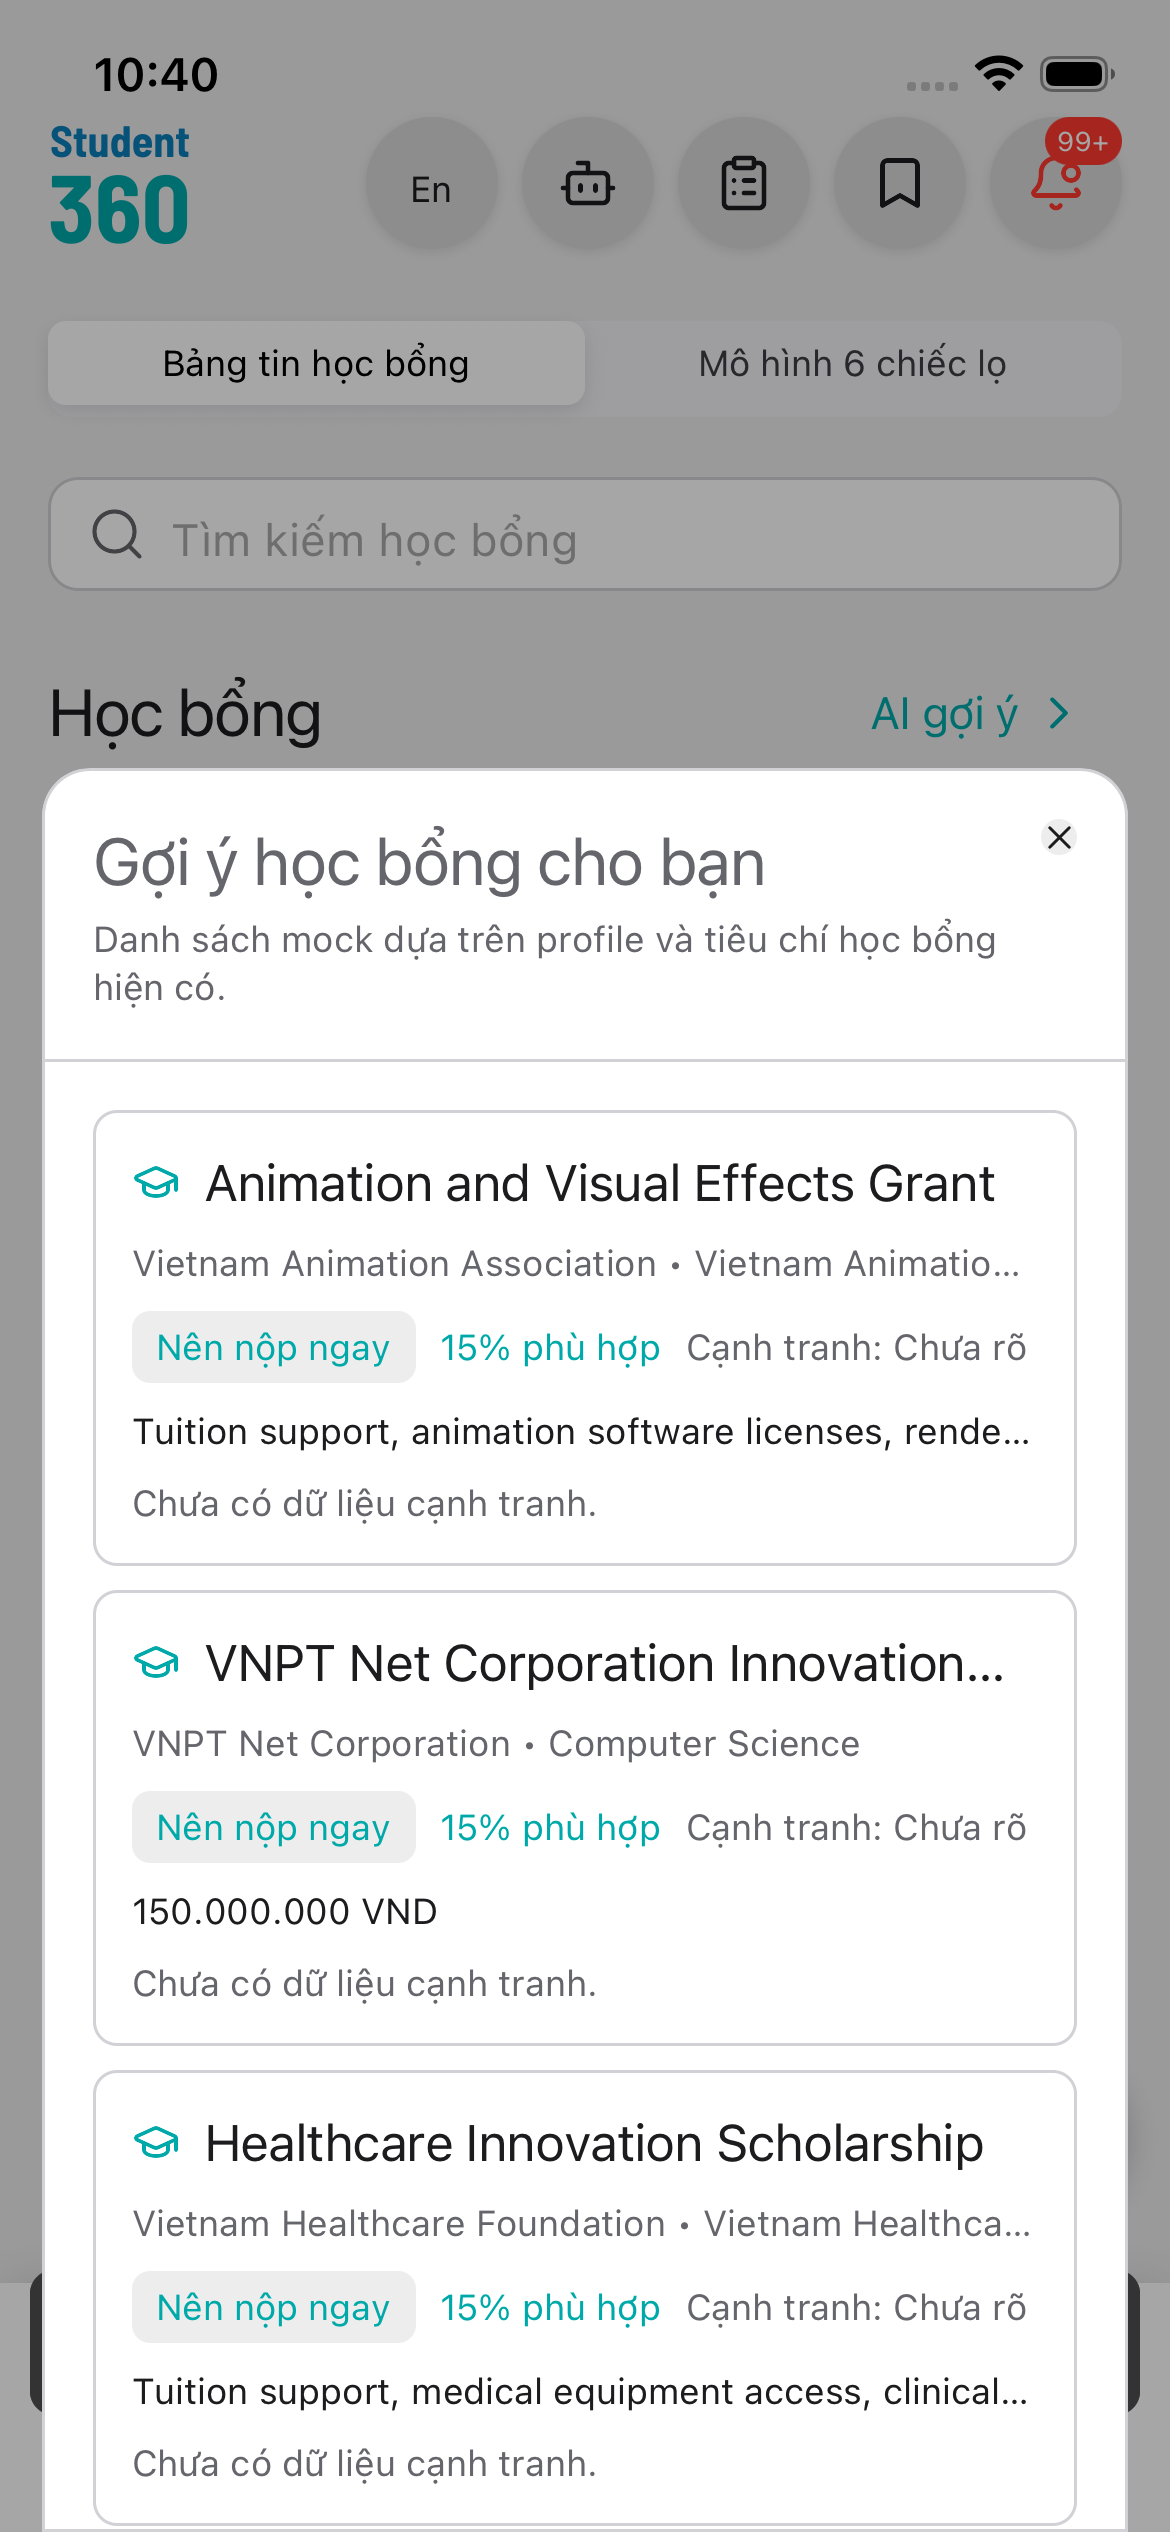
\includegraphics[width=\textwidth]{images/chapter4/mobile/H5.14-2.png}%
        }{%
            \rectbox{Gợi ý học bổng 2}
        }
        \centerline{(b) Chi tiết điểm khớp hồ sơ}
    \end{minipage}
    \caption{Giao diện gợi ý học bổng thông minh, xếp hạng theo điểm khớp hồ sơ}
    \label{fig:mobile-schol-match}
\end{figure}

\begin{figure}[H]
    \noindent\textbf{10.} \textbf{Chi tiết học bổng và Nộp hồ sơ:} Màn hình này hiển thị các thông tin chi tiết về học bổng (tiêu chuẩn, số lượng, giá trị và hạn nộp) và biểu mẫu nộp hồ sơ đăng ký. Sinh viên có thể tải lên các file tài liệu minh chứng (PDF/hình ảnh) trực tiếp từ điện thoại.
    
    \vspace{0.2cm}
    \centering
    \begin{minipage}{0.44\textwidth}
        \centering
        \IfFileExists{images/chapter4/mobile/scholarship-apply.png}{%
            
\includegraphics[width=\textwidth]{images/chapter4/mobile/scholarship-apply.png}%
        }{%
            \rectbox{Hình ảnh màn hình chi tiết học bổng trên Mobile}
        }
        \caption{Giao diện chi tiết học bổng trên thiết bị di động}
        \label{fig:mobile-scholarship-apply}
    \end{minipage}
    \hfill
    \begin{minipage}{0.44\textwidth}
        \centering
        \IfFileExists{images/chapter4/mobile/scholarship-apply-form.png}{%
            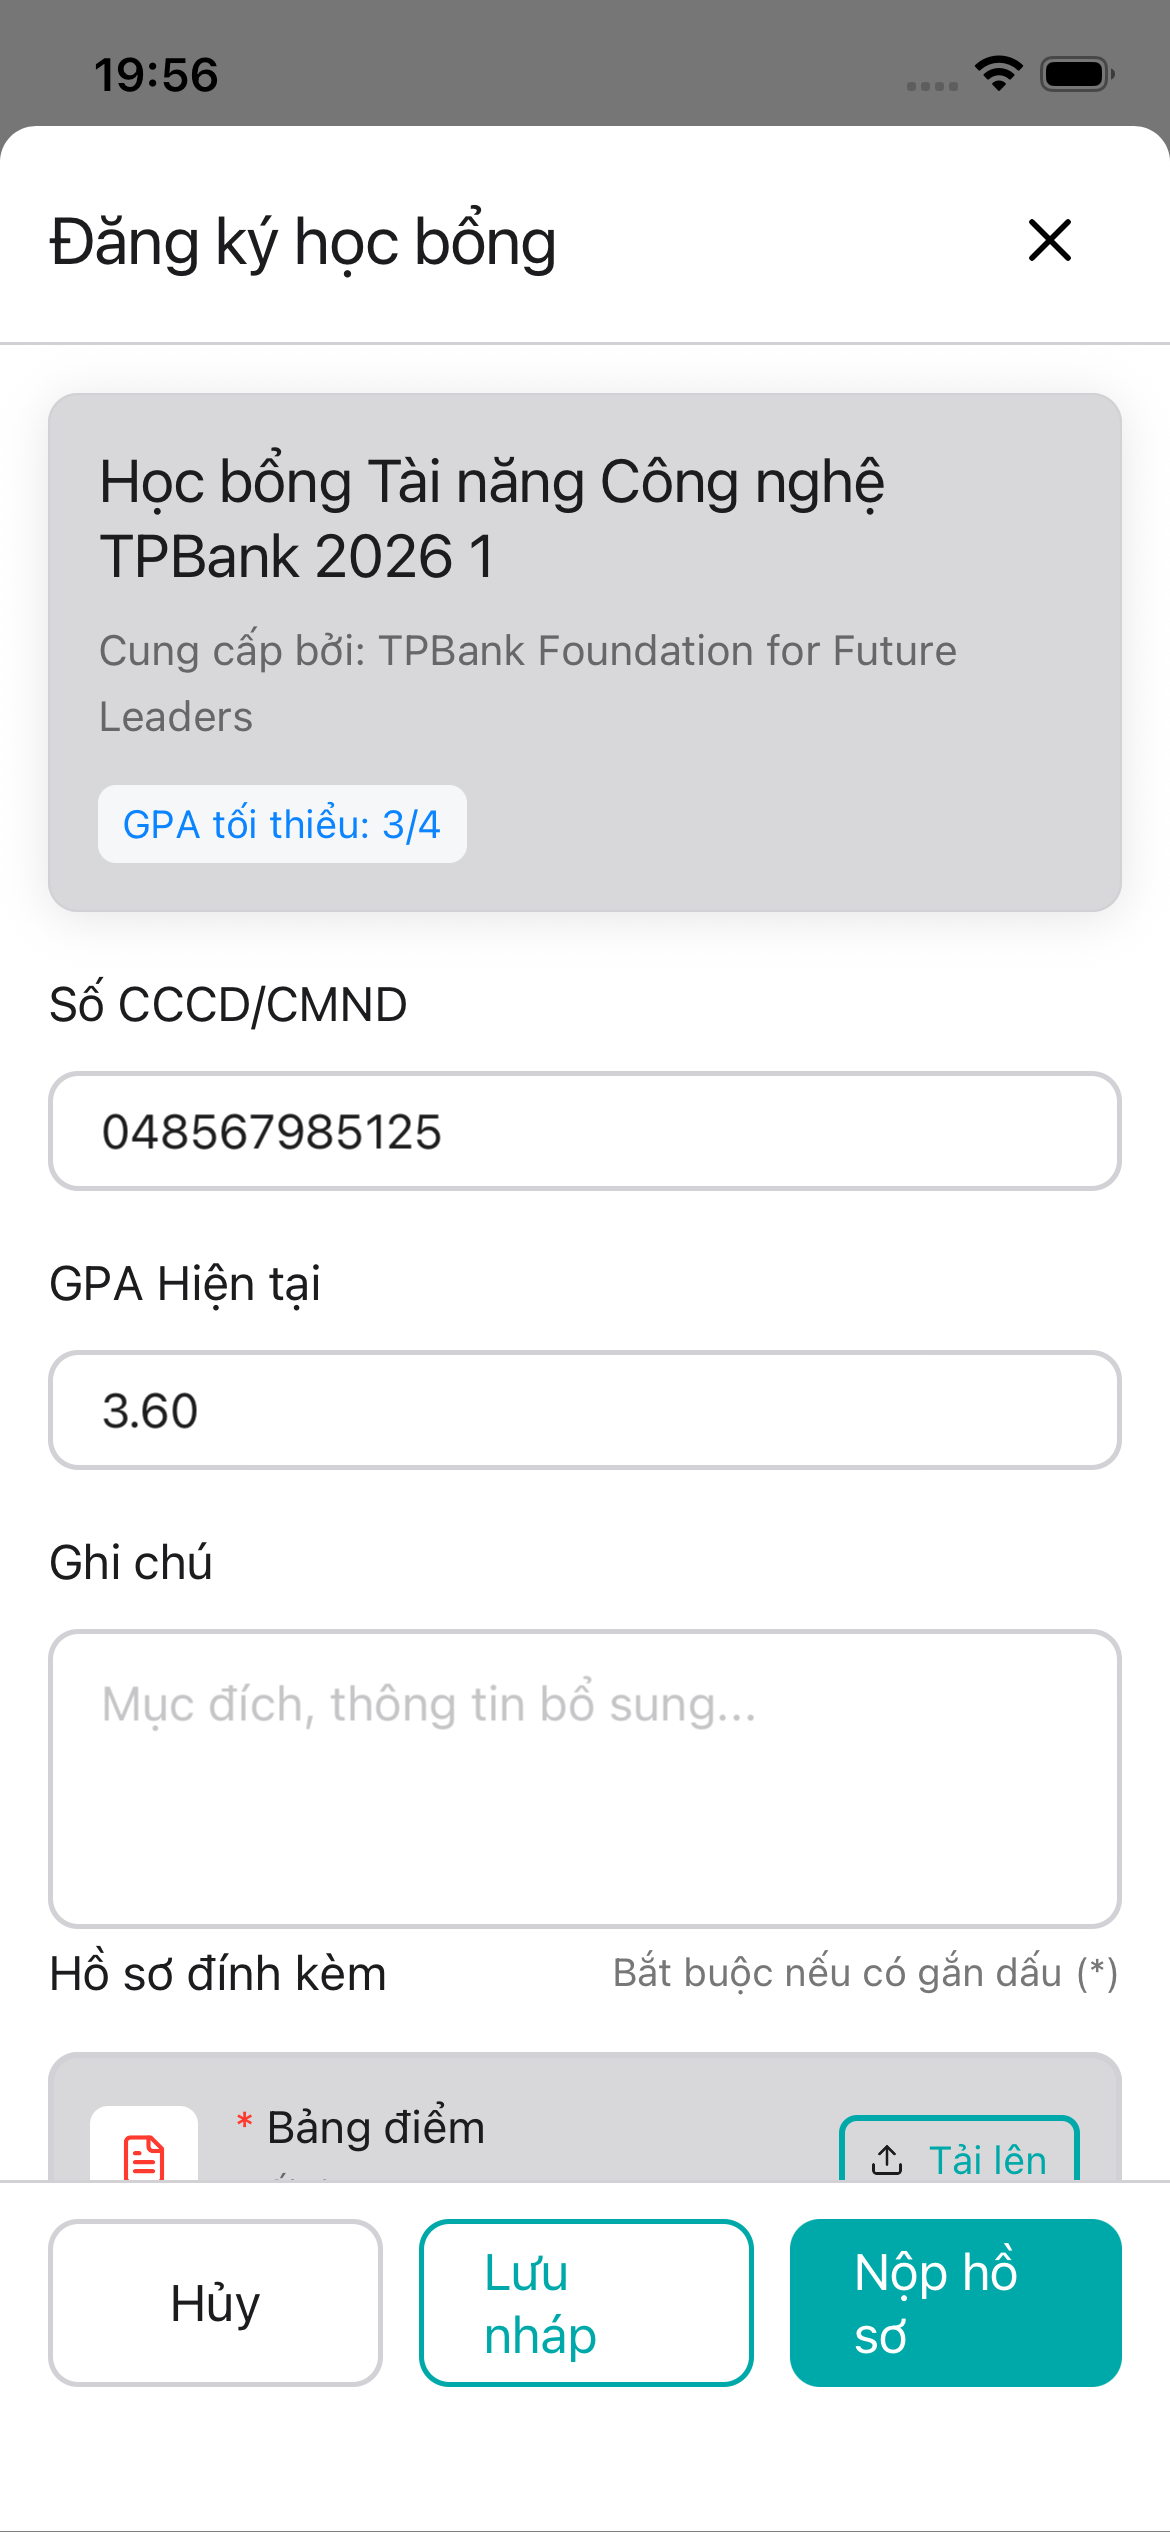
\includegraphics[width=\textwidth]{images/chapter4/mobile/scholarship-apply-form.png}%
        }{%
            \rectbox{Hình ảnh form đăng ký nộp hồ sơ học bổng trên Mobile}
        }
        \caption{Biểu mẫu đăng ký và nộp hồ sơ học bổng}
        \label{fig:mobile-scholarship-apply-form}
    \end{minipage}
\end{figure}
\clearpage

\begin{figure}[H]
    \noindent\textbf{11.} \textbf{Bảng điểm sinh viên:} Màn hình này hiển thị chi tiết kết quả học tập của sinh viên, bao gồm điểm trung bình tích lũy (GPA), tổng số tín chỉ đạt được và tiến độ đạt mục tiêu tốt nghiệp.
    
    \vspace{0.2cm}
    \centering
    \begin{minipage}{0.44\textwidth}
        \centering
        \IfFileExists{images/chapter4/mobile/gradebook-dashboard.png}{%
            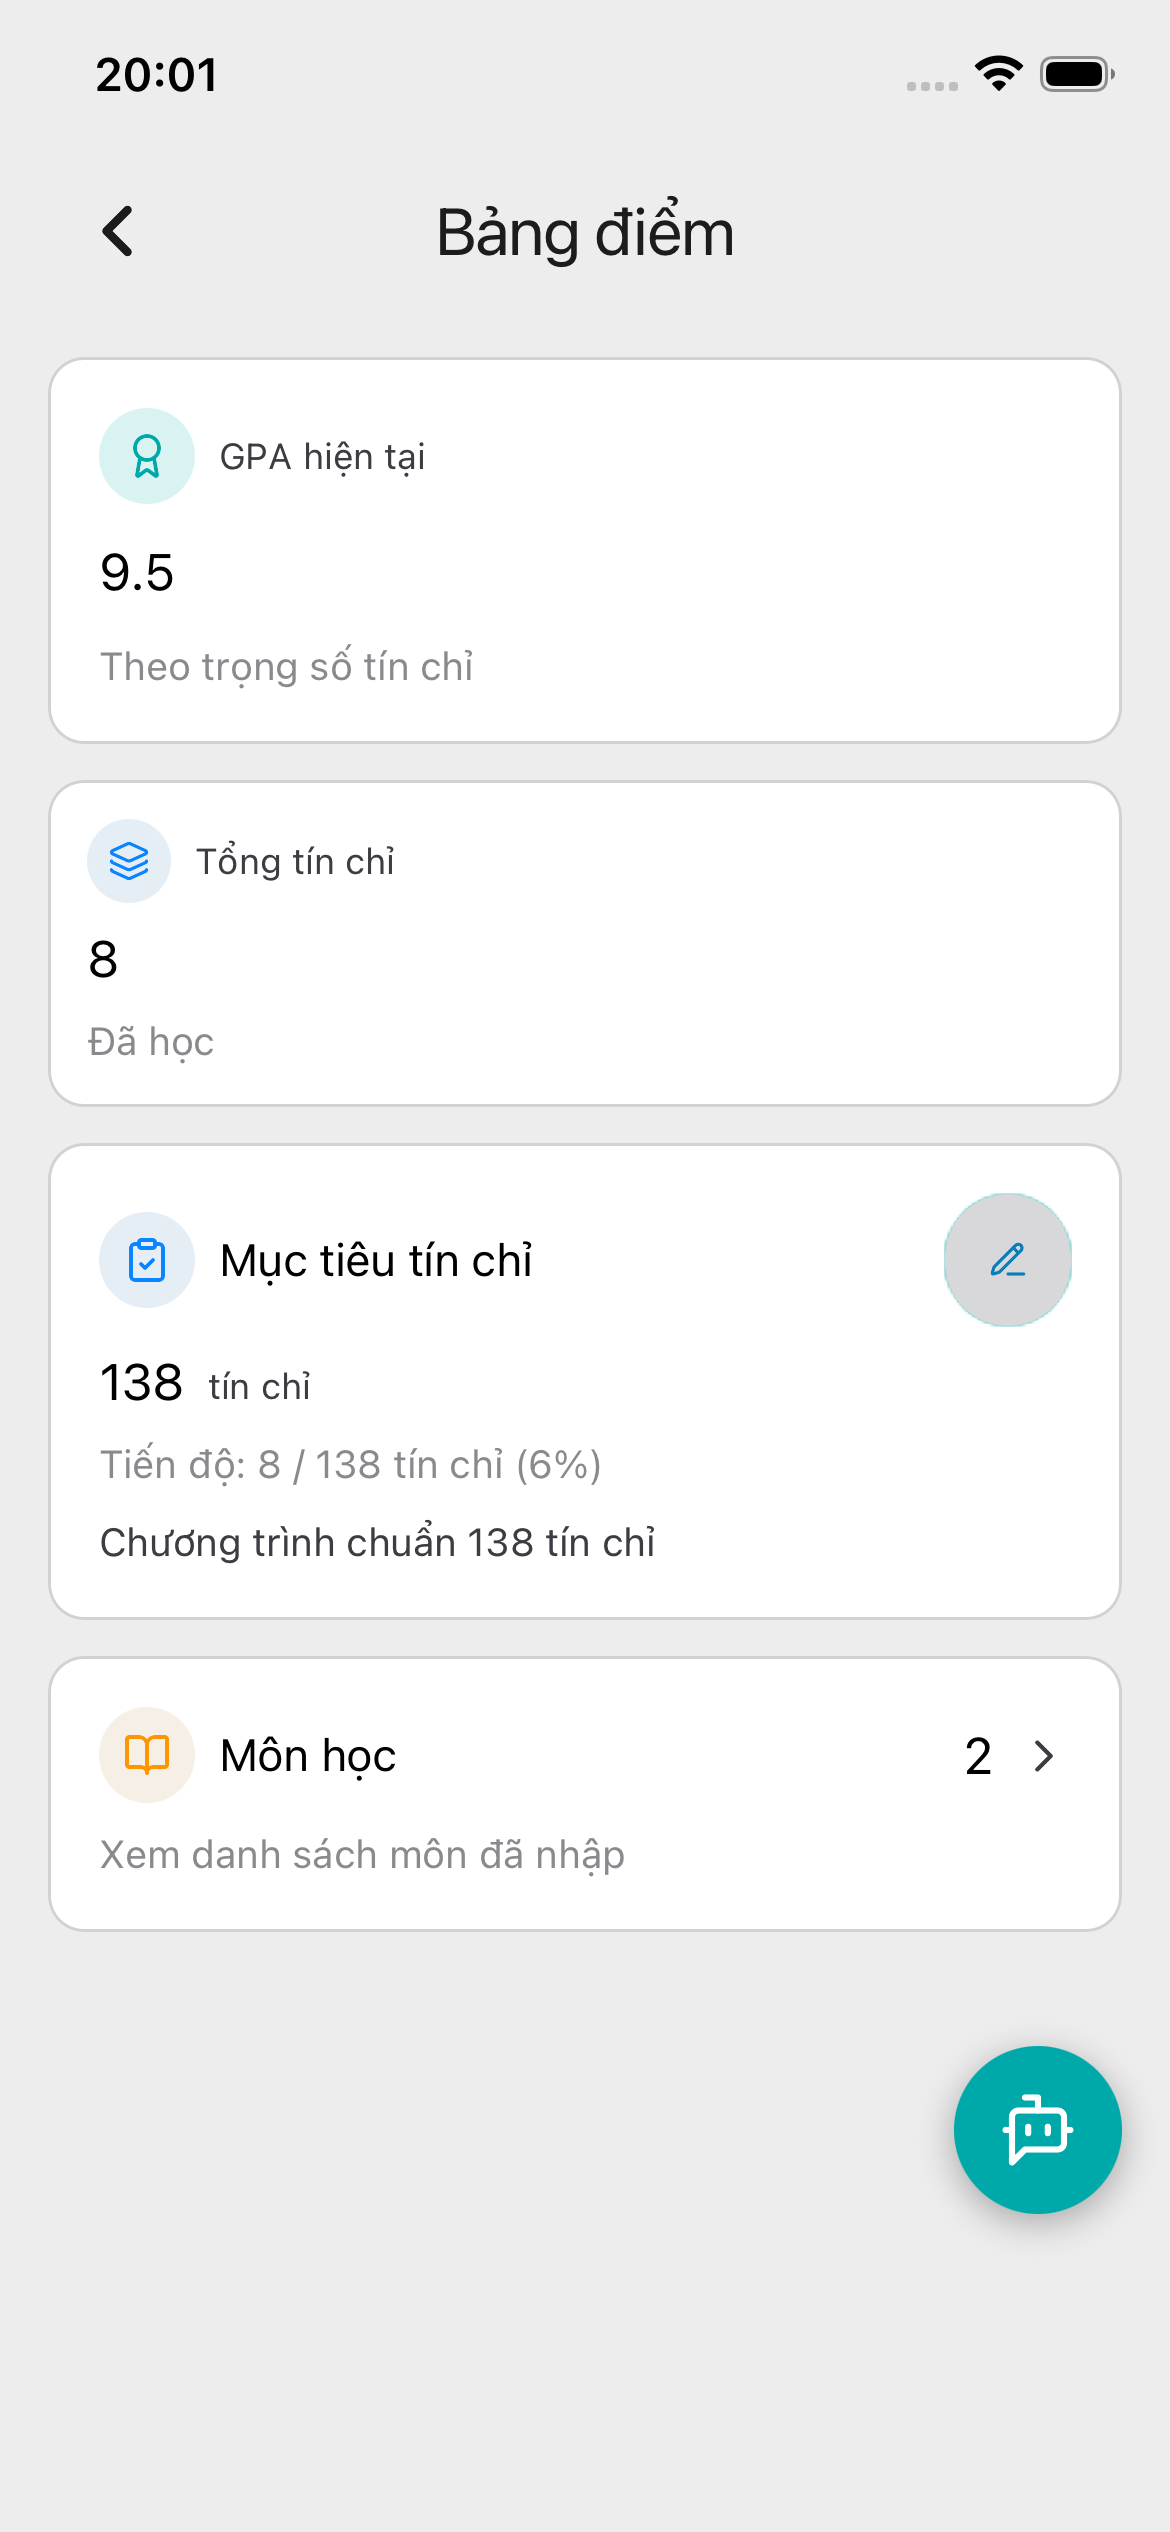
\includegraphics[width=\textwidth]{images/chapter4/mobile/gradebook-dashboard.png}%
        }{%
            \rectbox{Màn hình dashboard bảng điểm, GPA và mục tiêu tín chỉ trên Mobile}
        }
        \caption{Giao diện bảng điểm và tiến độ tín chỉ của sinh viên}
        \label{fig:mobile-gradebook-dashboard}
    \end{minipage}
    \hfill
    \begin{minipage}{0.44\textwidth}
        \centering
        \IfFileExists{images/chapter4/mobile/gradebook-courses.png}{%
            
\includegraphics[width=\textwidth]{images/chapter4/mobile/gradebook-courses.png}%
        }{%
            \rectbox{Màn hình thêm môn học và import bảng điểm TXT/CSV trên Mobile}
        }
        \caption{Giao diện nhập và import điểm sinh viên}
        \label{fig:mobile-gradebook-courses}
    \end{minipage}
\end{figure}

\begin{figure}[H]
    \noindent\textbf{12.} \textbf{Nhập môn và Import bảng điểm:} Màn hình này cho phép sinh viên nhanh chóng cập nhật bảng điểm bằng cách chọn trực tiếp môn học từ danh mục đào tạo chuẩn của trường đối tác, hoặc tải lên tệp văn bản (TXT/CSV) kết quả học tập để hệ thống tự động trích xuất điểm và số tín chỉ.

    \vspace{0.2cm}
    \centering
    \begin{minipage}{0.44\textwidth}
        \centering
        \IfFileExists{images/chapter4/mobile/H5.12-1.png}{%
            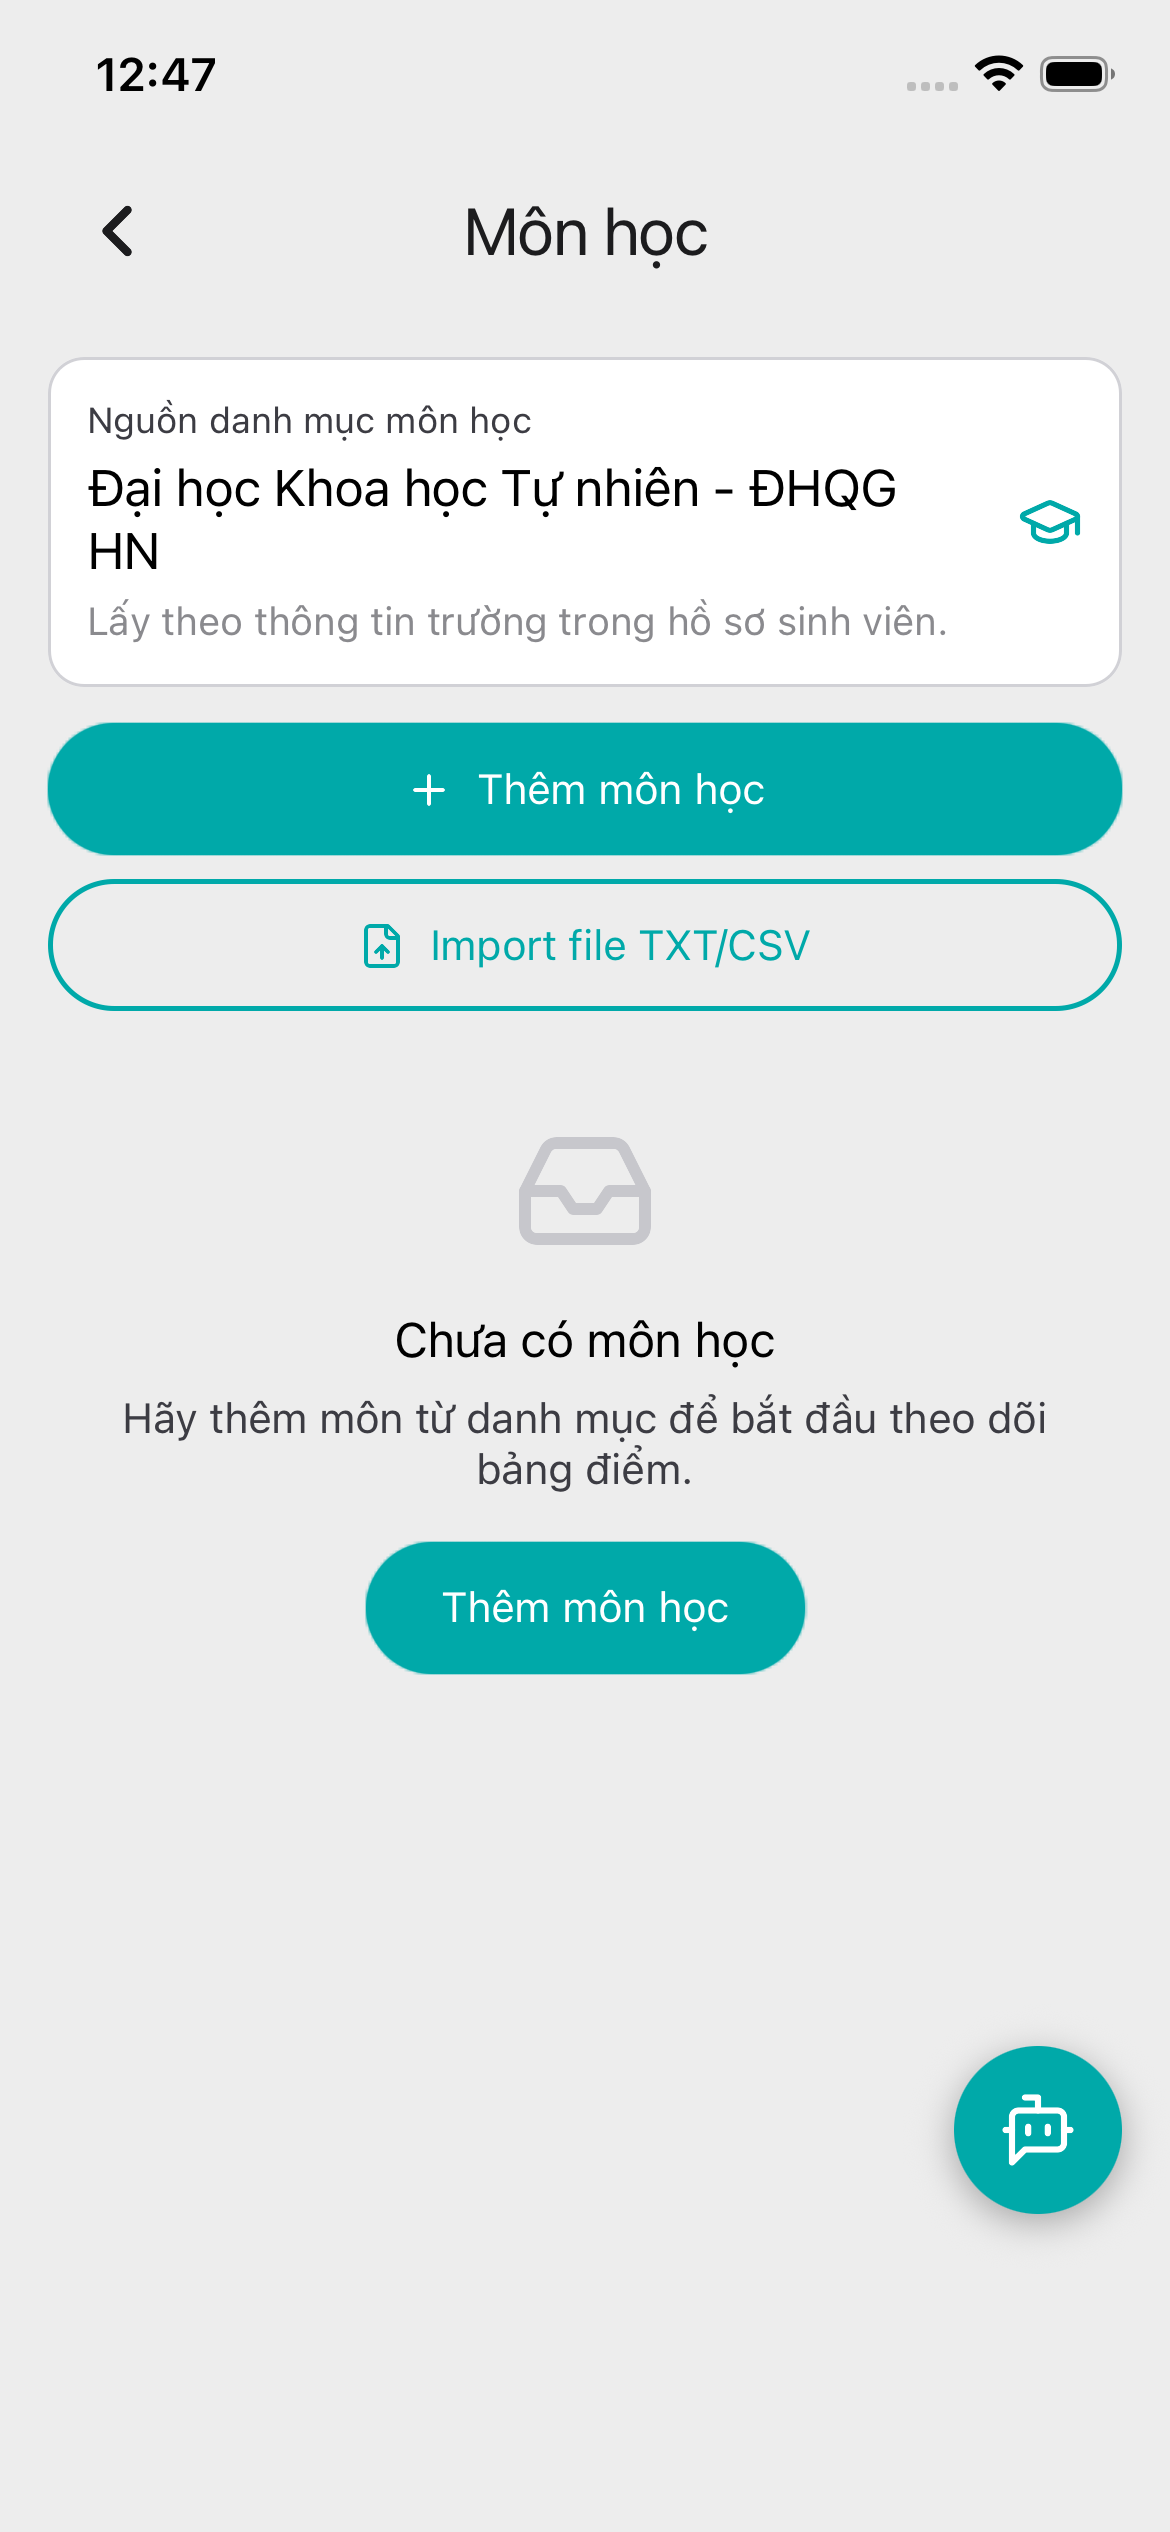
\includegraphics[width=\textwidth]{images/chapter4/mobile/H5.12-1.png}%
        }{%
            \rectbox{Màn hình chọn môn học từ danh mục chuẩn}
        }
        \caption{Giao diện thêm môn học và import bảng điểm}
        \label{fig:mobile-gradebook-add-subject}
    \end{minipage}
    \hfill
\end{figure}
\clearpage

\subsection{Webadmin quản trị hệ thống}
Giao diện quản trị Webadmin được xây dựng bằng React JS kết hợp Material UI (MUI), tối ưu cho việc hiển thị bảng dữ liệu lớn và xử lý quy trình phê duyệt.

\begin{enumerate}
    \item \textbf{Quản lý Trường đối tác:} Màn hình này cho phép quản trị viên xem, thêm mới hoặc điều chỉnh danh sách các trường đại học liên kết trong hệ thống để quản trị danh mục đào tạo.
    
    \begin{figure}[H]
        \centering
        \IfFileExists{images/chapter4/webadmin/universities.png}{%
            
\includegraphics[width=0.85\textwidth]{images/chapter4/webadmin/universities.png}%
        }{%
            \rectbox{Màn hình danh sách trường đại học trên Webadmin}
        }
        \caption{Giao diện quản lý danh mục trường đại học (thêm/sửa qua modal, tìm kiếm theo từ khóa)}
        \label{fig:webadmin-universities}
    \end{figure}
    \clearpage

    \item \textbf{Quản lý Môn học và Khoa:} Màn hình này dùng để quản lý chi tiết danh mục khoa, chương trình đào tạo và môn học tương ứng của từng trường đại học đối tác nhằm phục vụ cho chức năng quản lý bảng điểm của sinh viên.
    
    \begin{figure}[H]
        \centering
        \IfFileExists{images/chapter4/webadmin/subjects-programs.png}{%
            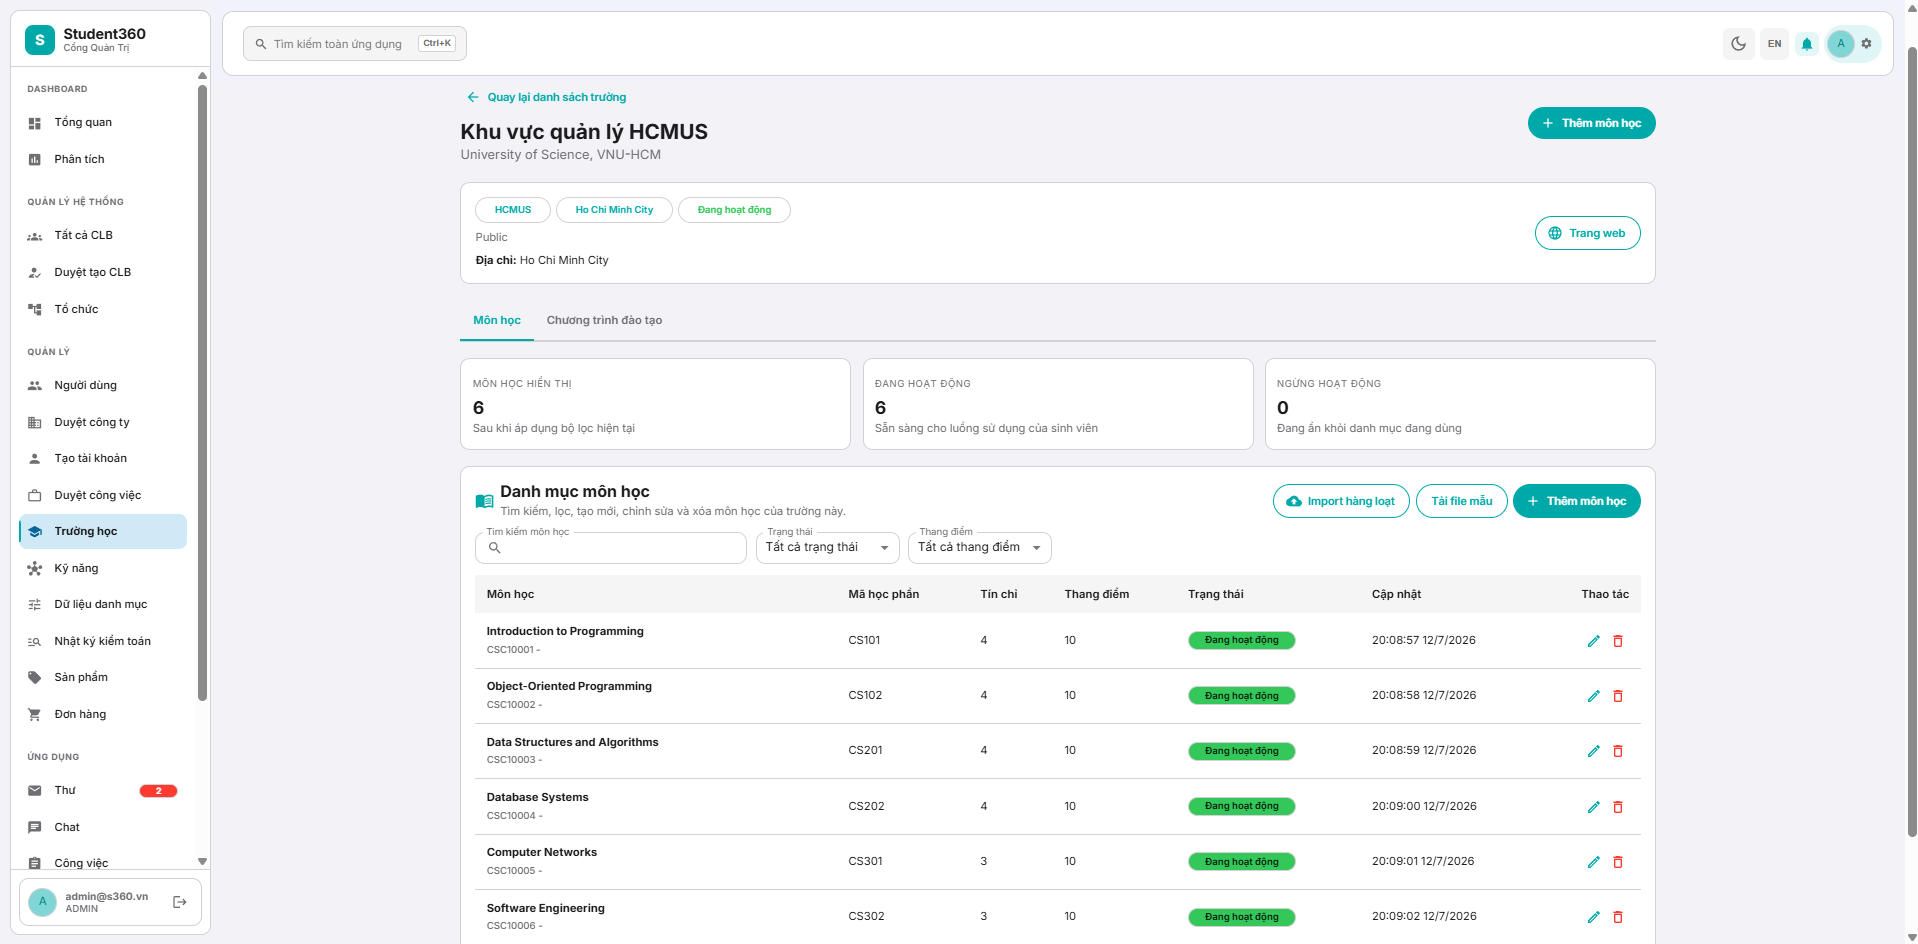
\includegraphics[width=0.85\textwidth,height=0.35\textheight,keepaspectratio]{images/chapter4/webadmin/subjects-programs.png}%
        }{%
            \rectbox{Màn hình quản lý môn học theo trường}
        }

        \vspace{0.4cm}

        \IfFileExists{images/chapter4/webadmin/training-programs.png}{%
            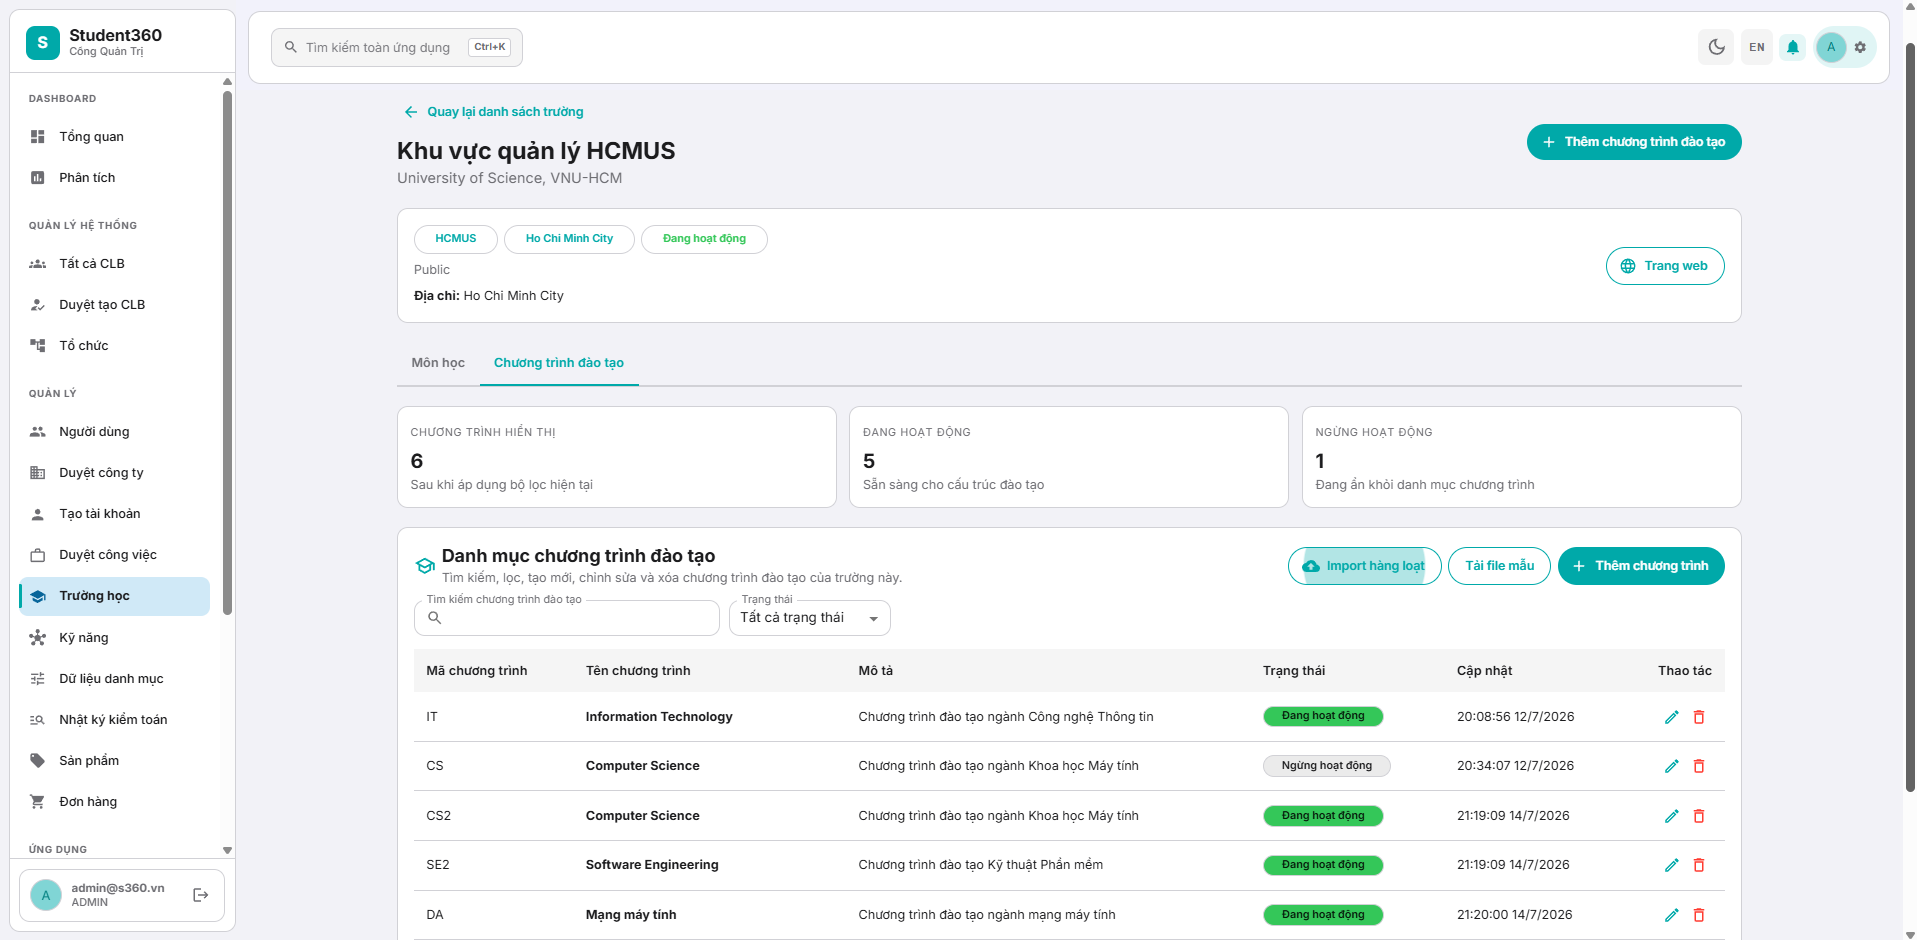
\includegraphics[width=0.85\textwidth,height=0.35\textheight,keepaspectratio]{images/chapter4/webadmin/training-programs.png}%
        }{%
            \rectbox{Màn hình quản lý khoa/chương trình đào tạo theo trường}
        }
        \caption{Giao diện quản lý môn học và khoa/chương trình đào tạo (hỗ trợ bulk import)}
        \label{fig:webadmin-subjects-programs}
    \end{figure}
    \clearpage

    \item \textbf{Danh sách Học bổng:} Màn hình này giúp các nhà tài trợ theo dõi danh sách toàn bộ các chương trình học bổng do mình tài trợ, cũng như tổng hợp số lượng hồ sơ đã ứng tuyển để tiến hành chấm điểm phê duyệt.
    
    \begin{figure}[H]
        \centering
        \IfFileExists{images/chapter4/webadmin/scholarships-list.png}{%
            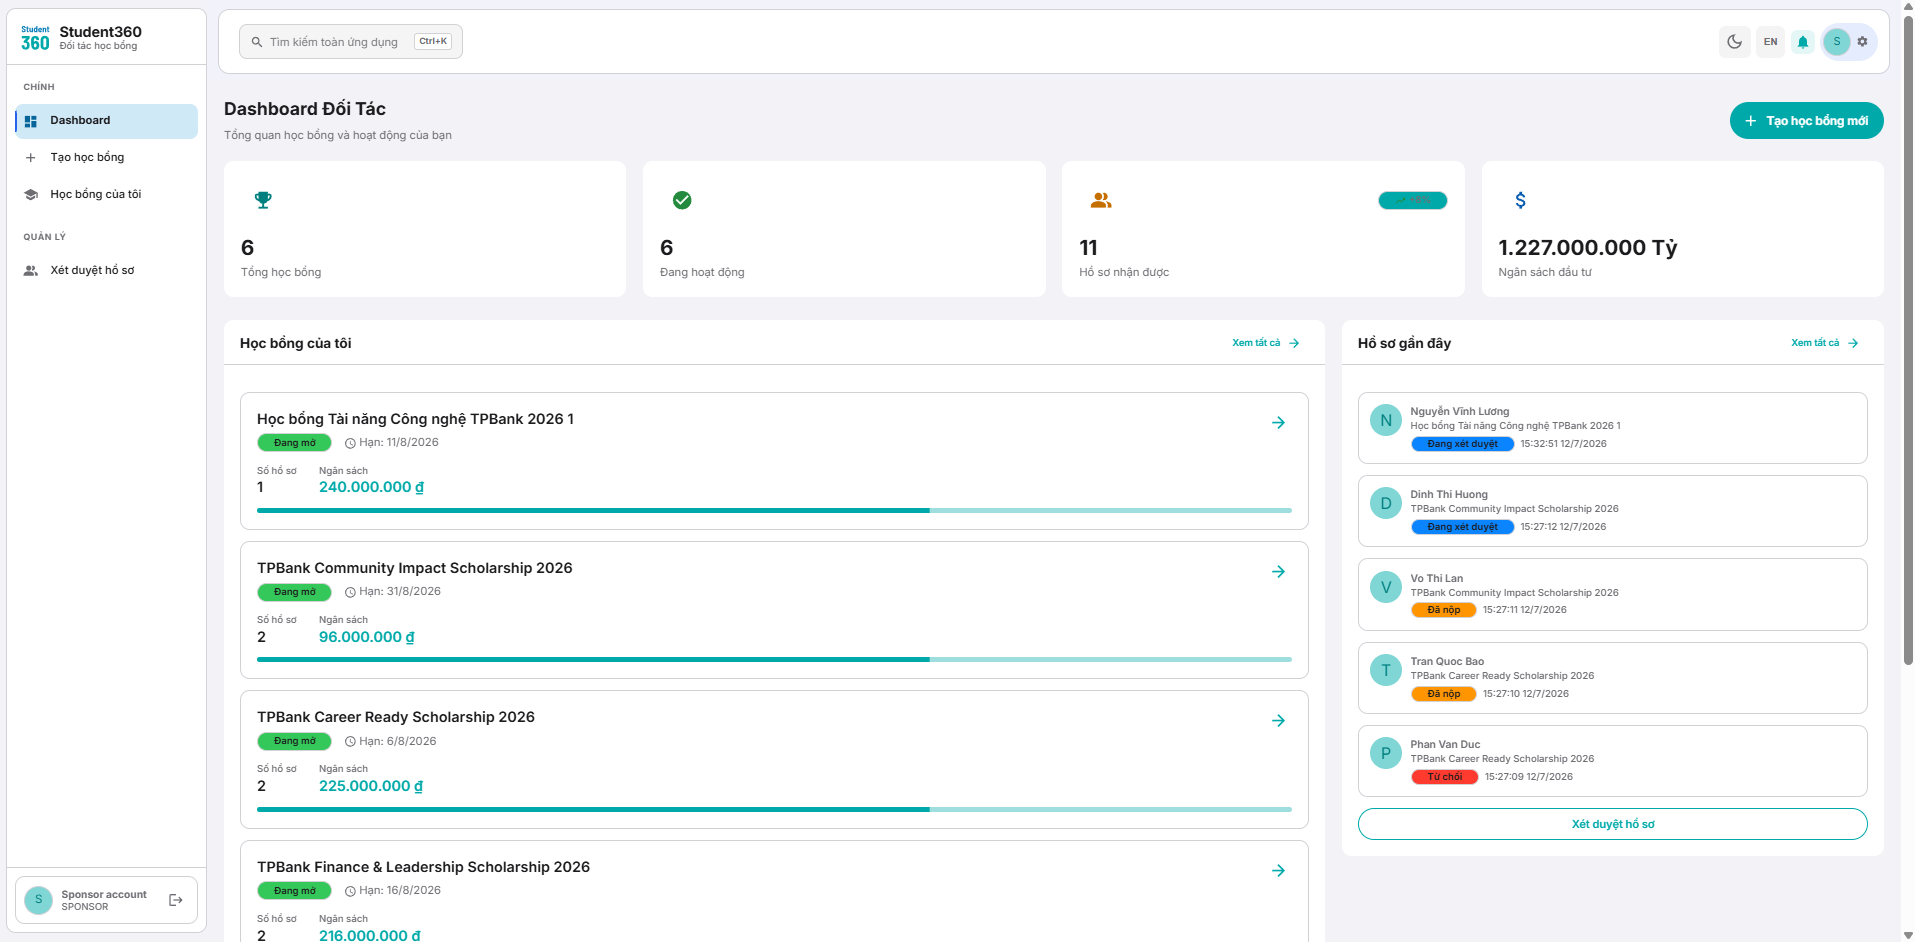
\includegraphics[width=0.85\textwidth]{images/chapter4/webadmin/scholarships-list.png}%
        }{%
            \rectbox{Màn hình danh sách Học bổng trên Webadmin}
        }
        \caption{Giao diện quản lý danh sách Học bổng, kèm thống kê tiến độ ứng tuyển}
        \label{fig:webadmin-scholarships-list}
    \end{figure}
    \clearpage

    \item \textbf{Tạo và Thiết lập Học bổng:} Màn hình này cung cấp biểu mẫu nhiều bước cho nhà tài trợ để xuất bản chương trình học bổng mới, thiết lập thông tin chung, giá trị giải thưởng và các tiêu chí lọc hồ sơ (như GPA tối thiểu, ngành học yêu cầu).
    
    \begin{figure}[H]
        \centering
        \IfFileExists{images/chapter4/webadmin/sponsor-create-scholarship-1.png}{%
            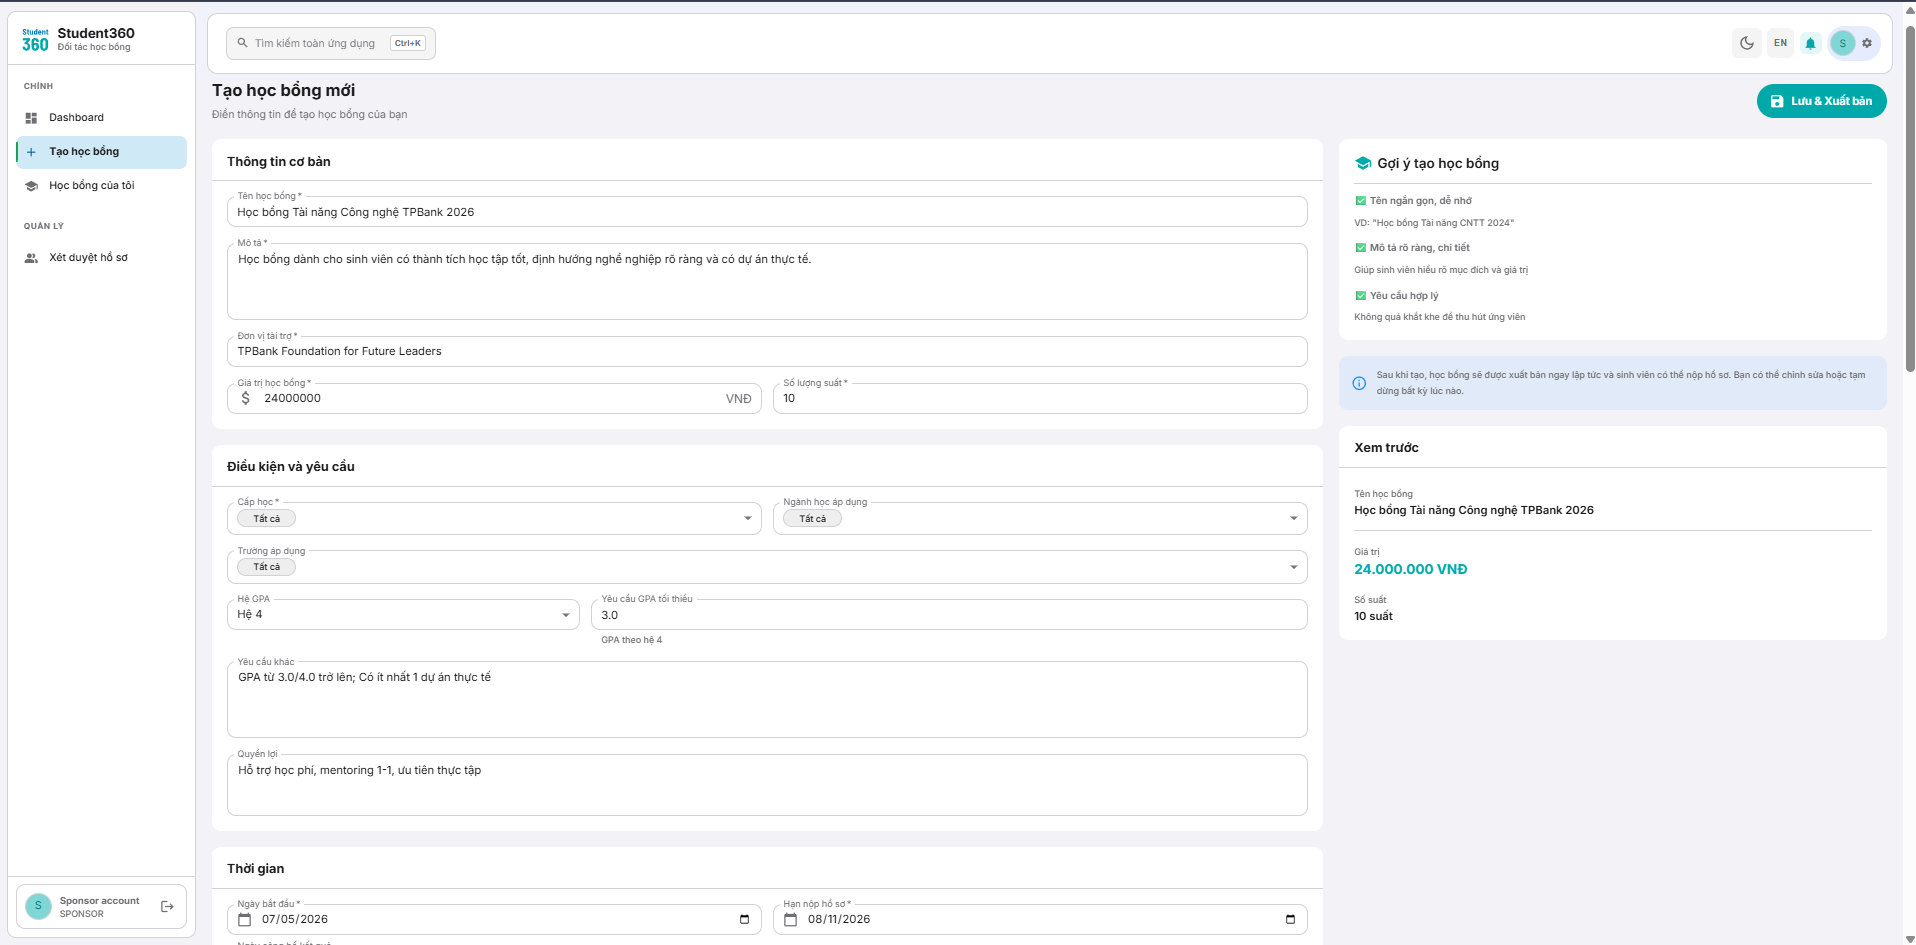
\includegraphics[width=0.85\textwidth]{images/chapter4/webadmin/sponsor-create-scholarship-1.png}%
        }{%
            \rectbox{Màn hình tạo học bổng - phần thông tin chung}
        }

        \vspace{0.4cm}

        \IfFileExists{images/chapter4/webadmin/sponsor-create-scholarship-2.png}{%
            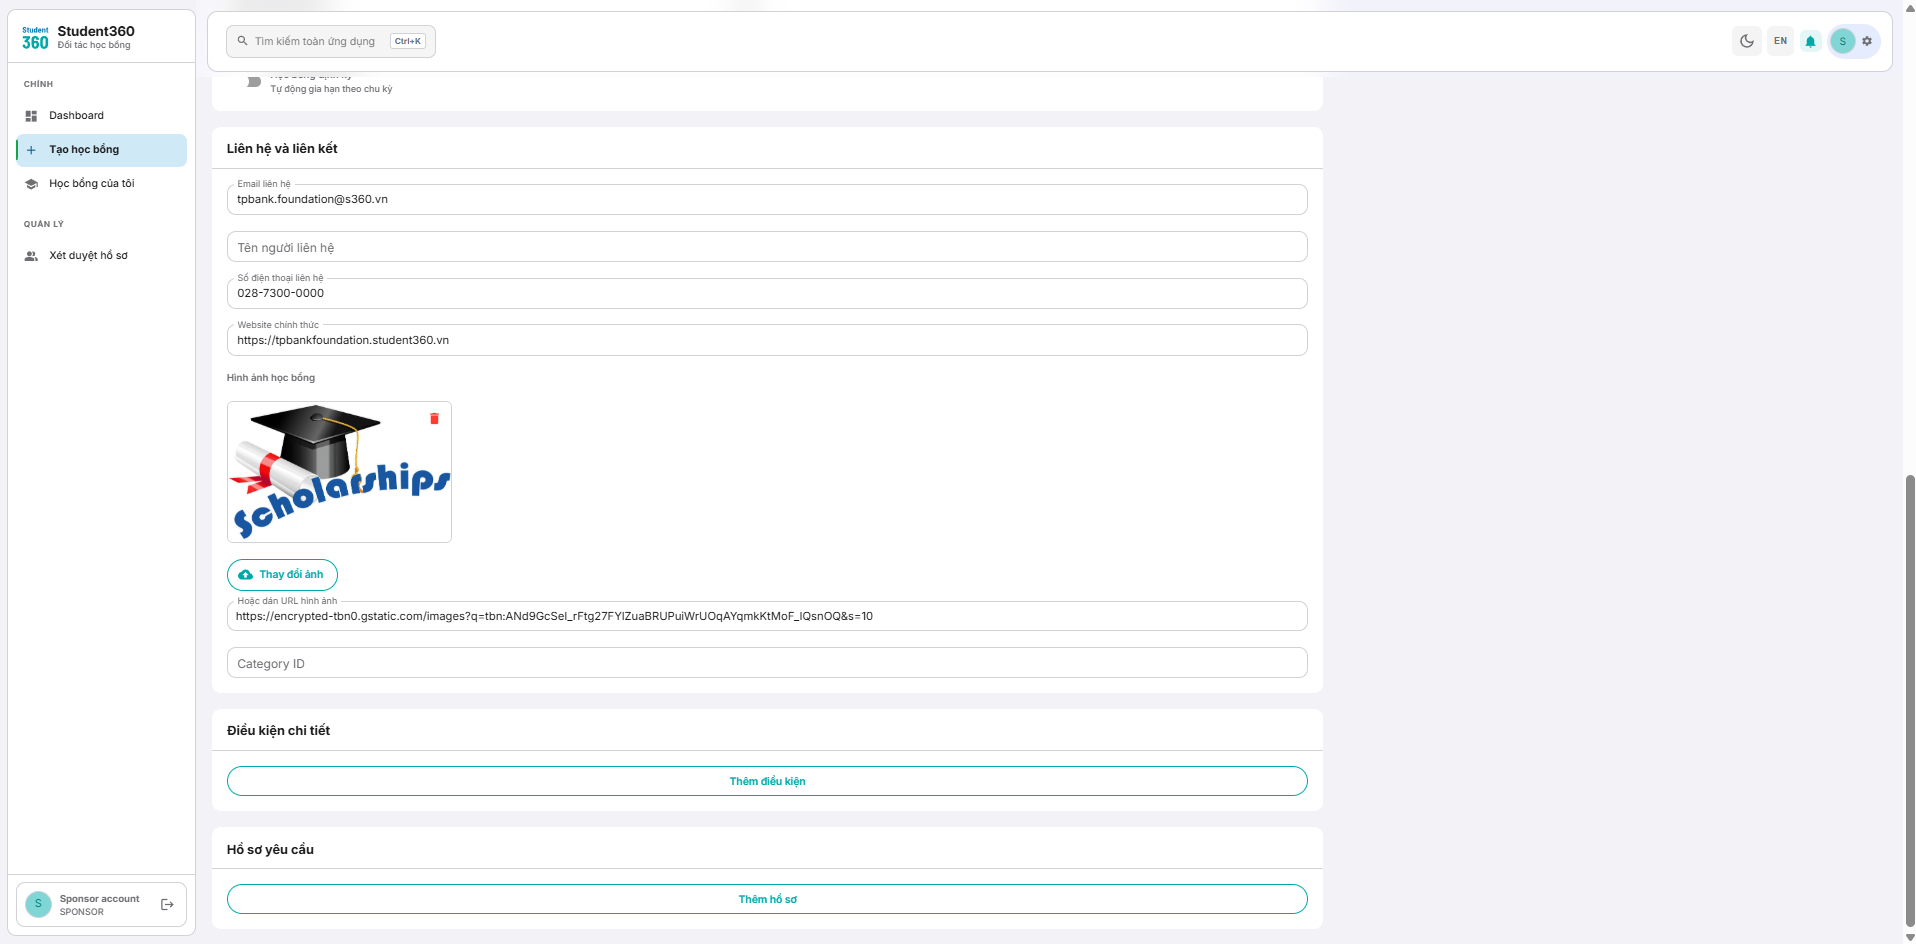
\includegraphics[width=0.85\textwidth]{images/chapter4/webadmin/sponsor-create-scholarship-2.png}%
        }{%
            \rectbox{Màn hình tạo học bổng - phần điều kiện xét tuyển}
        }

        \caption{Giao diện tạo và cấu hình học bổng dành cho nhà tài trợ}
        \label{fig:sponsor-create-scholarship}
    \end{figure}
    \clearpage

    \item \textbf{Xét duyệt hồ sơ học bổng:} Màn hình này cho phép nhà tài trợ xem chi tiết hồ sơ đăng ký của từng sinh viên (GPA, bảng điểm, tài liệu đính kèm) để phê duyệt hoặc từ chối đơn ứng tuyển kèm theo nhận xét phản hồi.
    
    \begin{figure}[H]
        \centering
        \IfFileExists{images/chapter4/webadmin/sponsor-application-review.png}{%
            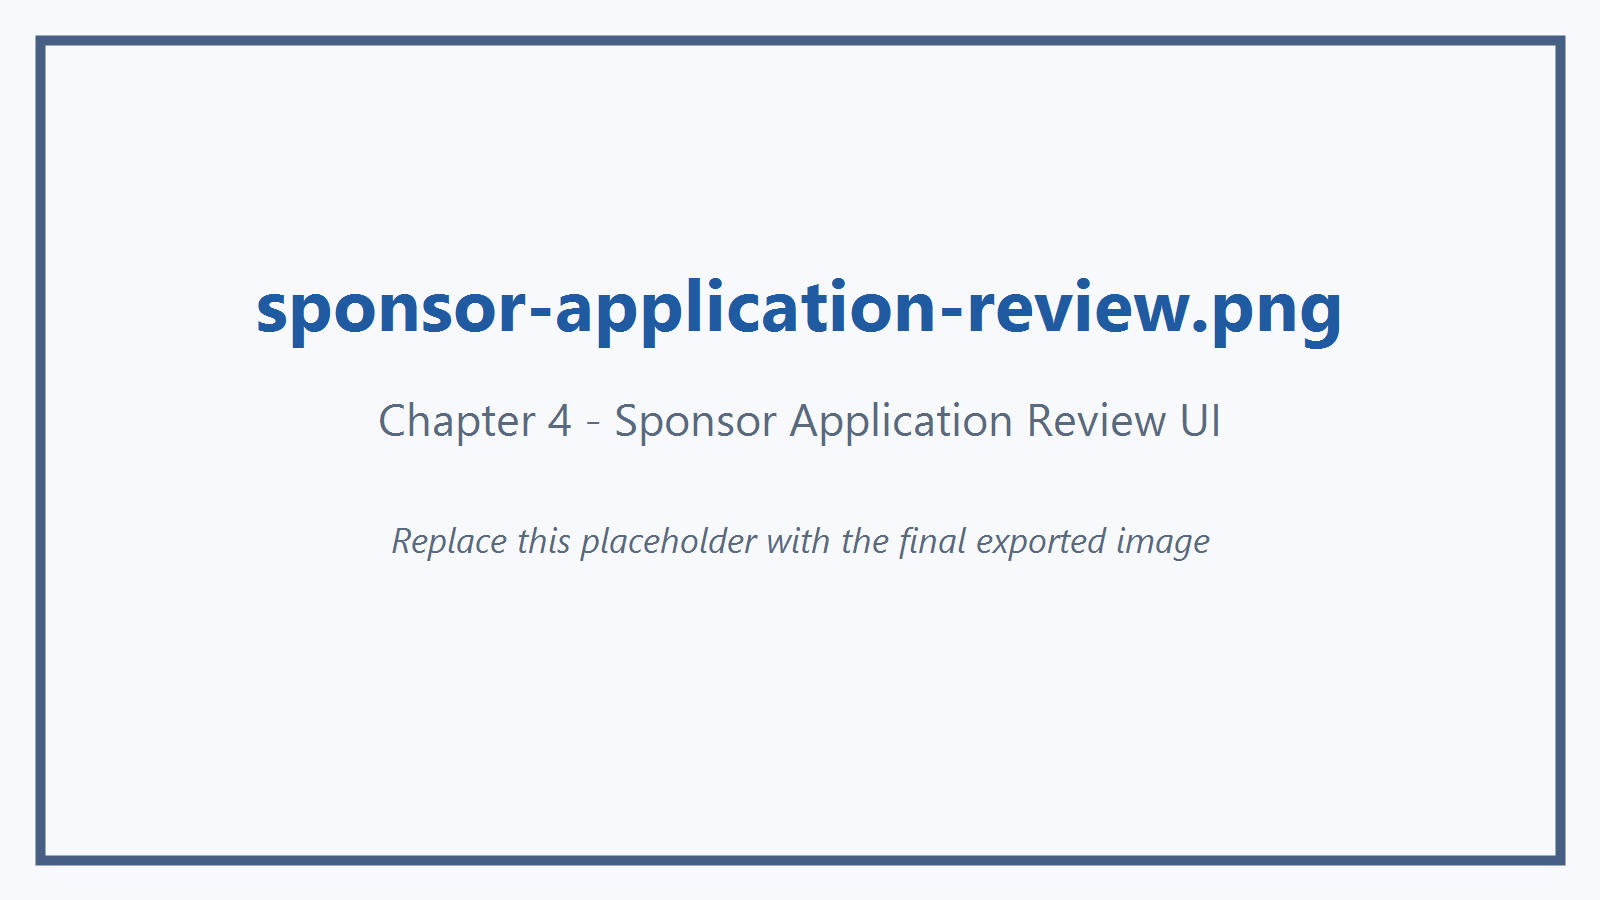
\includegraphics[width=0.85\textwidth]{images/chapter4/webadmin/sponsor-application-review.png}%
        }{%
            \rectbox{Màn hình xét duyệt hồ sơ ứng tuyển học bổng trên Webadmin}
        }
        \caption{Giao diện xét duyệt hồ sơ ứng tuyển học bổng (Duyệt/Từ chối kèm nhận xét)}
        \label{fig:sponsor-application-review}
    \end{figure}
\end{enumerate}


\section{Kiểm thử đơn vị}
\label{sec:kiem-thu-don-vi}
Kiểm thử đơn vị xác minh độc lập từng quy tắc nghiệp vụ của Phân hệ Quản lý Tài chính -- 6 hũ, giao dịch tài chính, cảnh báo tài chính, lịch chuyển tiền tự động, phân loại giao dịch bằng AI, khoản vay và học bổng -- mà không phụ thuộc PostgreSQL, Redis hay AI Service đang chạy: toàn bộ tầng lưu trữ dữ liệu, kết nối cơ sở dữ liệu và mô hình ngôn ngữ đều được giả lập (mock). Phía Backend và AI Service đều dùng bộ công cụ kiểm thử tự động theo đúng ngôn ngữ lập trình tương ứng, với dữ liệu và các dịch vụ ngoài được giả lập hoàn toàn. Không có tài khoản hay hạ tầng ngoài nào được sử dụng ở tầng kiểm thử này.

\subsection{Kết quả kiểm thử đơn vị}
Bảng~\ref{tab:unit-test-summary} tổng hợp kết quả chạy trên cả hai dịch vụ.

\begin{table}[H]
    \centering
    \begin{tabular}{|L{3.6cm}|L{4.2cm}|C{2.2cm}|C{2.2cm}|C{2.8cm}|}
        \hline
        \textbf{Dịch vụ} & \textbf{Phạm vi giả lập} & \textbf{Số bộ kiểm thử} & \textbf{Số test case} & \textbf{Kết quả} \\ \hline
        Backend (NestJS) & Toàn bộ tầng lưu trữ dữ liệu & 48 & 879 & \textbf{879/879 đạt} \\ \hline
        AI Service (FastAPI) & Cơ sở dữ liệu và mô hình ngôn ngữ & 8 & 95 & \textbf{95/95 đạt} \\ \hline
        \textbf{Tổng cộng} & & \textbf{56} & \textbf{974} & \textbf{974/974 đạt (100\%)} \\ \hline
    \end{tabular}
    \caption{Kết quả kiểm thử đơn vị theo dịch vụ}
    \label{tab:unit-test-summary}
\end{table}

Phía Backend, 48 bộ kiểm thử (879 test case) bao phủ toàn bộ các nhóm chức năng của Phân hệ Quản lý Tài chính: quản lý hũ tài chính (kể cả tích hợp AI, phân loại), giao dịch tài chính, cảnh báo tài chính, lịch chuyển tiền tự động, cổng giao tiếp với trợ lý AI, khoản vay, học bổng (từ danh mục, hồ sơ đến quy trình xét duyệt) và quản trị danh mục học thuật.

Phía AI Service, 8 nhóm kiểm thử (95 test case) bao phủ: gắn tag ngân sách cho hành động AI, nhận diện ý định hành động một chạm (one-touch execution), phát hiện bất thường chi tiêu, tổng hợp câu trả lời chat khi công cụ tra cứu trả dữ liệu thô, phân loại giao dịch (ưu tiên bảng tùy chọn cá nhân hóa, ngưỡng độ tin cậy, dự phòng khi mô hình lỗi), phân tích độ phù hợp học bổng, và công thức tính điểm sức khỏe tài chính (tỷ lệ chi tiêu, mức trừ điểm khi có bất thường mức độ nguy hiểm hoặc cảnh báo). Không phát sinh trường hợp nào thất bại ở cả hai dịch vụ.

\subsection{Độ bao phủ mã nguồn (Coverage)}
Độ bao phủ mã nguồn được đo riêng cho các nhóm chức năng thuộc phạm vi Phân hệ Quản lý Tài chính (không tính toàn bộ mã nguồn Backend). Bảng~\ref{tab:unit-test-coverage} trình bày kết quả.

\begin{table}[H]
    \centering
    \begin{tabular}{|L{4.4cm}|C{2.4cm}|C{2.4cm}|C{2.4cm}|C{2.4cm}|}
        \hline
        \textbf{Nhóm chức năng} & \textbf{Statements} & \textbf{Lines} & \textbf{Functions} & \textbf{Branch} \\ \hline
        Quản lý hũ tài chính & 88.99\% & 89.03\% & 96.55\% & 83.87\% \\ \hline
        Lịch chuyển tiền tự động & 93.54\% & 94.79\% & 95.91\% & 84.06\% \\ \hline
        Cảnh báo tài chính & 89.11\% & 92.80\% & 100.0\% & 81.52\% \\ \hline
        Giao dịch tài chính & 93.44\% & 93.88\% & 93.02\% & 90.40\% \\ \hline
        Khoản vay & 85.55\% & 86.90\% & 100.0\% & 100.0\% \\ \hline
        Học bổng & 82.92\% & 82.42\% & 70.38\% & 83.18\% \\ \hline
        Kết nối dịch vụ AI & 81.81\% & 86.20\% & 100.0\% & 100.0\% \\ \hline
        Cổng giao tiếp với trợ lý AI & 80.47\% & 81.25\% & 82.02\% & 70.64\% \\ \hline
        \textbf{Trung bình (8 nhóm chức năng Tài chính)} & \textbf{86.02\%} & \textbf{86.54\%} & \textbf{79.36\%} & \textbf{79.45\%} \\ \hline
    \end{tabular}
    \caption{Độ bao phủ mã nguồn theo nhóm chức năng (phạm vi Phân hệ Quản lý Tài chính)}
    \label{tab:unit-test-coverage}
\end{table}

Hầu hết các nhóm chức năng đều đạt trên 80\% ở cả bốn chỉ số, cho thấy các nhánh xử lý chính đã được kiểm chứng đầy đủ. Cổng giao tiếp với trợ lý AI có Branch coverage thấp hơn phần còn lại (70.64\%) do một phần mã nguồn thuộc các luồng phụ trợ (tư vấn nghề nghiệp, lộ trình học tập) nằm ngoài phạm vi Phân hệ Quản lý Tài chính -- các luồng nghiệp vụ tài chính cốt lõi trong cùng module (thực thi hành động một chạm, gợi ý học bổng qua hội thoại, quản lý phiên chat) đã được kiểm thử đầy đủ hơn.

\section{Kiểm thử tích hợp}
\label{sec:kiem-thu-tich-hop}
Kiểm thử tích hợp xác minh các tầng của hệ thống phối hợp đúng với nhau, ở hai mức độ khác nhau tuỳ đặc thù rủi ro của từng phần:

\begin{itemize}
    \item \textbf{Backend (NestJS):} Dựng tầng tiếp nhận yêu cầu thật (định tuyến, xác thực dữ liệu đầu vào, định dạng lỗi) cùng cơ chế xác thực đăng nhập thật; chỉ tầng xử lý nghiệp vụ (Service) bị giả lập. Cách dựng này đủ để phủ toàn bộ nhánh định tuyến, xác thực dữ liệu đầu vào, phân quyền và mã lỗi trả về mà không cần hạ tầng ngoài.
    \item \textbf{AI Service (FastAPI):} Gọi thẳng ứng dụng thật (không cần khởi động một máy chủ riêng) kết hợp \textbf{PostgreSQL thật}; chỉ mô hình ngôn ngữ (LLM) bị giả lập. Cách dựng này áp dụng cho các chức năng đọc/ghi trực tiếp cơ sở dữ liệu, nơi một câu lệnh truy vấn sai sẽ không thể phát hiện được nếu giả lập cơ sở dữ liệu.
\end{itemize}

\subsection{Kết quả kiểm thử tích hợp}
Bảng~\ref{tab:integration-test-summary} tổng hợp kết quả.

\begin{table}[H]
    \centering
    \begin{tabular}{|L{3.6cm}|L{4.6cm}|C{2.2cm}|C{2.2cm}|C{2.8cm}|}
        \hline
        \textbf{Dịch vụ} & \textbf{Cách dựng} & \textbf{Số bộ kiểm thử} & \textbf{Số test case} & \textbf{Kết quả} \\ \hline
        Backend (NestJS) & Tầng tiếp nhận yêu cầu thật, xử lý nghiệp vụ giả lập & 8 & 139 & \textbf{139/139 đạt} \\ \hline
        AI Service (FastAPI) & Ứng dụng thật, PostgreSQL thật, mô hình ngôn ngữ giả lập & 2 & 16 & \textbf{16/16 đạt} \\ \hline
        \textbf{Tổng cộng} & & \textbf{10} & \textbf{155} & \textbf{155/155 đạt (100\%)} \\ \hline
    \end{tabular}
    \caption{Kết quả kiểm thử tích hợp theo dịch vụ}
    \label{tab:integration-test-summary}
\end{table}

Bảng~\ref{tab:integration-test-backend-detail} liệt kê chi tiết 8 bộ kiểm thử tích hợp phía Backend theo phạm vi nghiệp vụ và trọng tâm kiểm chứng.

\begin{table}[H]
    \centering
    \small
    \begin{tabular}{|L{3.6cm}|L{5.4cm}|C{1.6cm}|L{4.0cm}|}
        \hline
        \textbf{Nhóm chức năng} & \textbf{Phạm vi nghiệp vụ được kiểm thử} & \textbf{Số case} & \textbf{Trọng tâm kiểm chứng} \\ \hline
        Khoản vay & Xem gói vay, xem chi tiết, đăng ký vay, xem khoản vay của tôi, hủy vay & 17 & Kiểm tra hợp lệ số tiền/kỳ hạn vay theo gói, từ chối khi chưa đăng nhập hoặc dữ liệu không hợp lệ \\ \hline
        Cảnh báo tài chính & Kích hoạt các loại cảnh báo (ngưỡng hũ, ngân sách, lịch sắp hết hạn, báo cáo tháng, nhắc giao dịch, bất thường) & 9 & Chuyển tham số đúng xuống cơ chế xử lý cảnh báo, từ chối khi chưa đăng nhập \\ \hline
        Học bổng & Tạo, cập nhật, nộp, xem trạng thái, hủy hồ sơ; đăng ký/hủy đăng ký chương trình & 24 & Vòng đời hồ sơ nháp → nộp → duyệt/hủy \\ \hline
        Quản trị học thuật & Quản lý danh mục trường đại học, môn học, chương trình đào tạo & 19 & Phân quyền (chỉ Quản trị viên), ràng buộc khi dữ liệu còn phụ thuộc \\ \hline
        Quản lý hũ tài chính & Danh sách, chi tiết, tạo, sửa, xoá, tỷ lệ phân bổ, gắn tag & 21 & Kiểm tra hợp lệ dữ liệu đầu vào, chặn sửa hũ hệ thống, chặn trùng tên \\ \hline
        Giao dịch tài chính & Danh sách, tổng hợp, tạo, phân bổ thu nhập, sửa, xoá & 20 & Kiểm tra hợp lệ dữ liệu đầu vào, chặn sửa giao dịch chuyển khoản \\ \hline
        Trợ lý AI & Trò chuyện, phiên chat, thực thi/xác nhận hành động, cảnh báo bất thường, xử lý phản hồi nội bộ từ AI Service & 22 & Xác thực nguồn gọi nội bộ, kiểm tra hợp lệ loại/tham số hành động \\ \hline
        Cảnh báo tài chính (dữ liệu thật) & Cơ chế chống trùng lặp cảnh báo, chạy trực tiếp trên PostgreSQL thật & 7 & Đúng ngữ nghĩa chống trùng lặp trong điều kiện tranh chấp \\ \hline
    \end{tabular}
    \caption{Chi tiết kiểm thử tích hợp Backend theo nhóm chức năng}
    \label{tab:integration-test-backend-detail}
\end{table}

Phía AI Service, 2 nhóm kiểm thử tích hợp (16 test case) chạm PostgreSQL thật: một nhóm 8 case cho chức năng cảnh báo bất thường (đọc/ghi thật bảng cảnh báo, lọc theo trạng thái đã đọc/loại cảnh báo, giới hạn phạm vi theo người dùng, từ chối khi thiếu/sai thông tin xác thực) và một nhóm 8 case cho chức năng phân loại giao dịch (khớp bảng tùy chọn cá nhân hóa thật, dự phòng qua mô hình ngôn ngữ khi không khớp, ngưỡng độ tin cậy, dự phòng về hũ mặc định khi mô hình lỗi).

\section{Quét lỗ hổng bảo mật mã nguồn}
\label{sec:kiem-thu-bao-mat}

Song song với kiểm thử chức năng, mã nguồn Backend được quét lỗ hổng bảo mật bằng công cụ \textbf{Trivy} nhằm đối chiếu các thư viện phụ thuộc của dự án với cơ sở dữ liệu lỗ hổng đã công bố (CVE), từ đó phát hiện sớm các rủi ro bảo mật từ bên thứ ba.

\subsection{Kỹ thuật khắc phục lỗ hổng bảo mật}
Để xử lý các lỗ hổng phát hiện bởi Trivy mà vẫn đảm bảo tính ổn định của ứng dụng, các kỹ thuật sau đã được áp dụng:

\begin{itemize}
    \item \textbf{Nâng cấp gói phụ thuộc trực tiếp:} Đối với các thư viện khai báo trực tiếp trong dự án, tiến hành cập nhật lên phiên bản đã được nhà phát triển vá lỗi bảo mật.
    \item \textbf{Ghi đè phiên bản gói phụ thuộc gián tiếp:} Đối với các lỗ hổng xuất phát từ thư viện con (được kéo vào bởi thư viện khác), áp dụng kỹ thuật ghi đè phiên bản (\textit{dependency overrides}) để buộc hệ thống sử dụng phiên bản an toàn.
    \item \textbf{Xác minh tính ổn định:} Sau khi áp dụng các biện pháp khắc phục, hệ thống được kiểm tra biên dịch lại và đóng gói để đảm bảo không phát sinh xung đột hay lỗi vận hành.
\end{itemize}

\subsection{Kết quả trước và sau khi khắc phục}
Bảng~\ref{tab:trivy-before-after} so sánh kết quả quét lỗ hổng bảo mật trước và sau khi áp dụng các biện pháp xử lý.

\begin{table}[H]
    \centering
    \begin{tabular}{|L{3.2cm}|C{3.2cm}|C{3.2cm}|}
        \hline
        \textbf{Mức độ nghiêm trọng} & \textbf{Trước khắc phục} & \textbf{Sau khắc phục} \\ \hline
        CRITICAL & 3 & \textbf{0} \\ \hline
        HIGH & 30 & \textbf{0} \\ \hline
        MEDIUM & 39 & \textbf{1} \\ \hline
        LOW & 7 & \textbf{1} \\ \hline
        \textbf{Tổng cộng} & \textbf{79} & \textbf{2} \\ \hline
    \end{tabular}
    \caption{Số lỗ hổng bảo mật mã nguồn theo mức độ nghiêm trọng trước và sau khắc phục}
    \label{tab:trivy-before-after}
\end{table}

Kết quả cho thấy toàn bộ các lỗ hổng ở mức nghiêm trọng (CRITICAL) và cao (HIGH) đã được khắc phục triệt để, tổng số lỗ hổng giảm từ 79 xuống còn 2. Hai lỗ hổng còn tồn đọng (1 MEDIUM, 1 LOW) được tạm thời chấp nhận rủi ro do một lỗ hổng đòi hỏi nâng cấp toàn bộ khung làm việc (NestJS) lên phiên bản mới và lỗ hổng còn lại hiện chưa có bản vá từ nhà phát triển.

\section{Đánh giá chất lượng và hiệu năng các chức năng AI}
\label{sec:danh-gia-ai}

\subsection{Phân loại giao dịch tự động}
\label{sec:kiem-thu-api}
Để tối ưu hóa chi phí vận hành và giảm thiểu độ trễ phản hồi, hệ thống áp dụng cơ chế phân loại hỗn hợp gồm hai bước (Hybrid Classification Pipeline):
\begin{itemize}
    \item \textbf{Bước 1 (Khớp từ khóa chính xác):} Hệ thống kiểm tra bảng tùy chọn cá nhân hóa của sinh viên trong cơ sở dữ liệu. Nếu khớp từ khóa (do người dùng từng xác nhận hoặc sửa đổi trước đây), hệ thống trả kết quả đề xuất hũ ngay lập tức mà không cần gọi mô hình AI.
    \item \textbf{Bước 2 (Dự phòng qua LLM):} Khi gặp từ khóa hoặc ngôn ngữ lóng mới, hệ thống gọi mô hình ngôn ngữ lớn để suy luận ngữ nghĩa và đề xuất hũ phù hợp. Khi người dùng xác nhận hoặc chỉnh sửa hũ tài chính thủ công trên giao diện, hệ thống tự động ghi nhận cặp từ khóa -- mã hũ này vào cơ sở dữ liệu, tạo thành một vòng tự học (self-learning loop) cá nhân hóa cho từng sinh viên.
\end{itemize}

\textit{Phương pháp đo:} Độ chính xác được đo trên bộ dữ liệu kiểm thử gồm 300 mô tả giao dịch tiếng Việt tự nhiên (50 mẫu cho mỗi hũ trong 6 hũ tài chính), chạy qua chức năng phân loại thật của hệ thống (Backend kết hợp AI Service), sau đó so khớp kết quả đề xuất với nhãn thực tế đã gán để tính các chỉ số độ chính xác. Bảng~\ref{tab:ai-classify-eval} và Bảng~\ref{tab:ai-classify-prf1} tổng hợp kết quả.

\begin{table}[H]
    \centering
    \begin{tabular}{|L{4.8cm}|C{2.6cm}|C{3.4cm}|C{2.8cm}|}
        \hline
        \textbf{Hũ tài chính} & \textbf{Tổng mẫu thử} & \textbf{Số mẫu phân loại đúng} & \textbf{Độ chính xác (Accuracy)} \\
        \hline
        Chi tiêu thiết yếu (essentials) & 50 & 46 & 92.0\% \\ \hline
        Giáo dục (education) & 50 & 49 & 98.0\% \\ \hline
        Đầu tư (investment) & 50 & 50 & 100.0\% \\ \hline
        Thiện tâm (sharing) & 50 & 50 & 100.0\% \\ \hline
        Hưởng thụ (enjoyment) & 50 & 49 & 98.0\% \\ \hline
        Tiết kiệm (reserve) & 50 & 50 & 100.0\% \\ \hline
        \textbf{Trung bình toàn hệ thống} & \textbf{300} & \textbf{294} & \textbf{98.0\%} \\
        \hline
    \end{tabular}

    \caption{Đánh giá độ chính xác phân loại giao dịch của AI theo hũ tài chính (N=300)}
    \label{tab:ai-classify-eval}
\end{table}

\begin{table}[H]
    \centering
    \begin{tabular}{|L{3.2cm}|C{2.4cm}|C{2.2cm}|C{2.2cm}|}
        \hline
        \textbf{Hũ tài chính} & \textbf{Precision} & \textbf{Recall} & \textbf{F1} \\
        \hline
        Chi tiêu thiết yếu & 100.0\% & 92.0\% & 95.8\% \\ \hline
        Giáo dục & 98.0\% & 98.0\% & 98.0\% \\ \hline
        Đầu tư & 100.0\% & 100.0\% & 100.0\% \\ \hline
        Thiện tâm & 100.0\% & 100.0\% & 100.0\% \\ \hline
        Hưởng thụ & 94.2\% & 98.0\% & 96.1\% \\ \hline
        Tiết kiệm & 96.2\% & 100.0\% & 98.0\% \\ \hline
        \multicolumn{4}{|l|}{Accuracy: \textbf{98.0\%}} \\ \hline
        \multicolumn{4}{|l|}{Macro-F1: \textbf{98.0\%}} \\ \hline
    \end{tabular}

    \caption{Precision / Recall / F1 theo từng hũ tài chính (N=300)}
    \label{tab:ai-classify-prf1}
\end{table}

Mô hình AI đạt độ chính xác \textbf{98.0\%} trên 300 mẫu thử nghiệm và Macro-F1 đạt 98.0\%. Hũ Tiết kiệm (reserve) đạt Accuracy tuyệt đối 100.0\%, không ghi nhận nhầm lẫn nào sang Đầu tư (investment) hay các hũ khác -- ranh giới ngữ nghĩa giữa hành vi cất giữ an toàn (tiết kiệm) và hành vi sinh lời (đầu tư) được phân định rõ. Số lỗi còn lại trong toàn bộ 300 mẫu chỉ chiếm 2.0\% (6/300) và phân bố rải rác, không tập trung vào một cặp hũ cụ thể: 2/50 mẫu Chi tiêu thiết yếu bị nhầm sang Hưởng thụ, 2/50 nhầm sang Tiết kiệm; 1/50 mẫu Giáo dục nhầm sang Hưởng thụ; 1/50 mẫu Hưởng thụ nhầm sang Giáo dục. Ba hũ đạt Accuracy tuyệt đối 100\% (Đầu tư, Thiện tâm, Tiết kiệm) -- trong phạm vi bộ dữ liệu đánh giá, pipeline phân loại đạt kết quả tốt và đồng đều trên cả 6 hũ tài chính, không có hũ nào là điểm yếu có tính hệ thống.

\subsection{Gợi ý học bổng}
\label{sec:danh-gia-hoc-bong}
\textit{Phương pháp đo:} Bộ dữ liệu kiểm thử gồm 150 hồ sơ sinh viên so khớp với 300 học bổng, mỗi hồ sơ được gán sẵn 25 học bổng thực sự phù hợp làm đáp án đúng để đối chiếu. Kết quả dưới đây đo trên chính hàm mà hệ thống dùng để trả danh sách gợi ý hiển thị cho người dùng (gồm bước lọc theo trường/ngành, sau đó sắp xếp theo điểm tổng hợp giữa độ liên quan chủ đề, mức phù hợp GPA và giá trị học bổng), thực thi cục bộ, không qua mạng hay gọi LLM, đảm bảo kết quả tất định và có thể tái lập.

Bảng~\ref{tab:scholarship-matching} tổng hợp kết quả, tính trung bình qua toàn bộ 150 hồ sơ.

\begin{table}[H]
    \centering
    \begin{tabular}{|L{9.0cm}|C{3.0cm}|}
        \hline
        \textbf{Chỉ số} & \textbf{Kết quả} \\ \hline
        Tỷ lệ hồ sơ có học bổng đúng ở vị trí gợi ý đầu tiên & \textbf{92.0\%} \\ \hline
        Tỷ lệ hồ sơ tìm thấy ít nhất 1 học bổng đúng trong 3 gợi ý đầu & \textbf{92.7\%} \\ \hline
        Tỷ lệ hồ sơ tìm thấy ít nhất 1 học bổng đúng trong 5 gợi ý đầu & \textbf{94.7\%} \\ \hline
        Số học bổng đúng trung bình xuất hiện trong 5 gợi ý đầu (trên tổng 25 học bổng đúng/hồ sơ) & \textbf{4.54/5} \\ \hline
        Tỷ lệ học bổng đúng không bị lọc nhầm ở bước lọc trường/ngành & \textbf{100.0\%} \\ \hline
    \end{tabular}
    \caption{Kết quả đánh giá gợi ý học bổng (N=150 hồ sơ, 300 học bổng, 25 học bổng đúng/hồ sơ)}
    \label{tab:scholarship-matching}
\end{table}

Bước lọc theo trường/ngành không loại nhầm bất kỳ học bổng phù hợp nào (100\%). Với 92.0\% hồ sơ, học bổng gợi ý đầu tiên đã là một lựa chọn đúng; 92.7\% hồ sơ tìm thấy ít nhất một học bổng phù hợp ngay trong 3 gợi ý đầu tiên và \textbf{94.7\% hồ sơ} tìm thấy học bổng thực sự phù hợp ngay trong 5 gợi ý đầu tiên -- tức là sinh viên gần như luôn thấy được một học bổng đúng mà không cần cuộn xem nhiều. Trung bình mỗi hồ sơ có 4.54 học bổng đúng xuất hiện trong 5 gợi ý đầu, cho thấy danh sách gợi ý không chỉ đúng ở vị trí đầu mà còn bao phủ tốt phần lớn các lựa chọn phù hợp khác.

\subsection{Trợ lý tư vấn tài chính (Chatbot AI)}
\textit{Phương pháp đo:} Bộ 184 câu hỏi tiếng Việt tự nhiên bao phủ 28 công cụ (tool) của trợ lý AI -- tra cứu số dư/ngân sách/giao dịch hũ, thống kê chi tiêu, lịch chuyển tự động, tư vấn khả năng chi trả và tái phân bổ hũ, gợi ý và tra cứu học bổng, hồ sơ ứng tuyển -- được gửi tuần tự qua tài khoản thật đến hệ thống đang chạy cục bộ (Backend + AI Service). Bảng~\ref{tab:chatbot-eval} tổng hợp kết quả.

\begin{table}[H]
    \centering
    \begin{tabular}{|L{5.0cm}|C{4.4cm}|}
        \hline
        \textbf{Chỉ số} & \textbf{Giá trị} \\ \hline
        Tổng số câu hỏi & 184 \\ \hline
        Trả lời thành công & \textbf{184/184 (100\%)} \\ \hline
        Timeout / lỗi & 0 \\ \hline
        Độ trễ trung bình & 16.3s \\ \hline
        Độ trễ P50 & 14.4s \\ \hline
        Độ trễ P95 & 38.0s \\ \hline
        Độ trễ P99 & 53.9s \\ \hline
        Độ trễ nhỏ nhất / lớn nhất & 0.9s / 65.9s \\ \hline
    \end{tabular}
    \caption{Kết quả kiểm thử trợ lý tư vấn tài chính AI (N=184)}
    \label{tab:chatbot-eval}
\end{table}

Toàn bộ 184 câu hỏi đều được trả lời hợp lệ, không phát sinh timeout hay lỗi thực thi. Với các câu hỏi dạng đếm/tổng số lượng (ví dụ ``có tổng cộng bao nhiêu học bổng trong hệ thống?''), cơ chế trả về của công cụ tra cứu có trường tổng số bản ghi thoả điều kiện độc lập với tham số giới hạn số lượng mà mô hình tự chọn khi gọi công cụ, giúp câu trả lời nhất quán qua nhiều lần hỏi lặp lại cùng nội dung. Đối chiếu độ trễ giữa môi trường cục bộ và môi trường triển khai thực tế (cùng 20 câu hỏi, cùng tài khoản) cho thấy môi trường ảnh hưởng đáng kể đến hình dạng phân bố độ trễ: môi trường triển khai thực tế có trung vị thấp hơn (4.6s so với 14.1s cục bộ) nhưng đuôi phân bố dài hơn rõ rệt (P95 đạt 74.0s so với 23.7s cục bộ), cho thấy phần lớn câu hỏi được xử lý rất nhanh nhưng một số ít câu chịu độ trễ mạng đáng kể.

\subsection{Chi phí vận hành AI}
\textit{Phương pháp đo:} Lượng token đầu vào/đầu ra và chi phí ước tính (theo đơn giá Gemini 2.5 Pro trên Vertex AI) được ghi nhận trực tiếp từ 62 lượt hỏi--đáp thật của trợ lý tư vấn tài chính, đối chiếu khớp với bảng ghi nhận sử dụng AI trong cơ sở dữ liệu hệ thống. Bảng~\ref{tab:ai-token-cost} tổng hợp kết quả.

\begin{table}[H]
    \centering
    \begin{tabular}{|L{5.6cm}|C{3.8cm}|}
        \hline
        \textbf{Chỉ số} & \textbf{Giá trị} \\ \hline
        Tổng số lượt hỏi--đáp & 62 (62/62 thành công) \\ \hline
        Tổng token đầu vào & 816.923 \\ \hline
        Tổng token đầu ra & 11.051 \\ \hline
        Tổng chi phí ước tính & 29.762,19 VND \\ \hline
        Token đầu vào trung bình / lượt & 13.176 \\ \hline
        Token đầu ra trung bình / lượt & 178 \\ \hline
        Chi phí trung bình / lượt & 480,04 VND \\ \hline
    \end{tabular}
    \caption{Chi phí token AI đo trên 62 lượt hỏi--đáp thật}
    \label{tab:ai-token-cost}
\end{table}

Ngoại suy tuyến tính từ mẫu đo được, chi phí vận hành ước tính (chưa gồm các lệnh gọi LLM phụ như phân loại ý định hay kiểm duyệt hành động) tăng theo tần suất sử dụng: khoảng 2.400 VND/người dùng/tháng ở mức 5 tin nhắn/tháng, khoảng 9.601 VND ở mức 20 tin nhắn/tháng, và khoảng 28.802 VND ở mức 60 tin nhắn/tháng -- tương ứng khoảng 2,4 đến 28,8 triệu VND/tháng cho quy mô 1.000 người dùng hoạt động. Công cụ tra cứu danh sách học bổng đầy đủ có chi phí token đầu vào cao gấp khoảng 4,4 lần trung bình chung do trả nguyên dữ liệu danh sách vào ngữ cảnh hội thoại, là công cụ tốn chi phí nhất trong 28 công cụ được đo.

\subsection{Hạn chế của đánh giá AI}
Các kết quả đánh giá AI trình bày ở trên phản ánh đúng phạm vi bộ dữ liệu và điều kiện thử nghiệm hiện tại, nhưng vẫn còn một số giới hạn cần lưu ý. Bộ dữ liệu đánh giá (300 mẫu phân loại giao dịch, 30 hồ sơ so khớp học bổng, 184 câu hỏi tư vấn) tuy đã được mở rộng so với các lần đo trước nhưng vẫn ở quy mô vừa phải so với dữ liệu thực tế phát sinh khi hệ thống có đông người dùng. Việc đánh giá cũng mới dừng ở dữ liệu thử nghiệm được xây dựng có chủ đích, chưa được kiểm chứng trên tập người dùng thật với hành vi và cách diễn đạt đa dạng hơn ở quy mô lớn. Ngoài ra, các chỉ số đo được (accuracy, Top-1, độ trễ) chưa được đối chiếu với một mô hình hay hệ thống tương tự khác để có cơ sở so sánh tương đối. Đây là những hướng cần tiếp tục thực hiện trong các giai đoạn phát triển tiếp theo của đề tài.

\section{Nhận xét và đánh giá tổng quan}

\subsection{Khả năng ứng dụng thực tiễn của hệ thống}
Hệ thống Student360 được thiết kế hướng đến khả năng đưa vào sử dụng thực tế cho đúng các bên liên quan trong hệ sinh thái giáo dục:
\begin{itemize}
    \item \textbf{Sẵn sàng triển khai cho trường đại học và nhà tài trợ:} Phân hệ Webadmin cho phép nhà trường quản lý danh mục đào tạo, môn học và bảng điểm; nhà tài trợ đăng chương trình học bổng và xét duyệt hồ sơ ứng tuyển ngay trên nền tảng, không cần quy trình giấy tờ hay trao đổi thủ công qua nhiều kênh riêng lẻ.
    \item \textbf{Khả năng mở rộng khi số lượng người dùng tăng:} Kiến trúc phân tách rõ ràng giữa ứng dụng di động, trang quản trị, Backend và AI Service theo từng dịch vụ độc lập, cho phép nâng cấp năng lực xử lý của từng thành phần riêng biệt khi lưu lượng sử dụng tăng, thay vì phải mở rộng toàn bộ hệ thống như kiến trúc nguyên khối.
    \item \textbf{Khả năng tích hợp thêm phân hệ mới:} Việc module hóa theo từng nhóm chức năng (tài chính, học thuật, học bổng, trợ lý AI) giúp bổ sung phân hệ mới hoặc mở rộng nghiệp vụ hiện có mà không ảnh hưởng đến các khối chức năng đang vận hành.
    \item \textbf{Có thể sử dụng ngay trong thực tế:} Toàn bộ luồng nghiệp vụ chính -- quản lý 6 hũ tài chính, theo dõi bảng điểm, tìm và ứng tuyển học bổng, trò chuyện với trợ lý AI -- đã được hiện thực hóa đầy đủ trên cả ứng dụng di động và trang quản trị, sẵn sàng để sinh viên, nhà trường và nhà tài trợ trải nghiệm trực tiếp.
\end{itemize}

\subsection{Đóng góp thực tiễn của sản phẩm đối với đối tượng đích}
Student360 không đơn thuần là một công cụ tiện ích riêng lẻ mà hướng tới việc tạo dựng một hệ sinh thái hỗ trợ sinh viên toàn diện:
\begin{itemize}
    \item \textbf{Giải quyết bài toán tài chính cá nhân gắn liền với học tập:} Khác với các app quản lý chi tiêu thông thường, Student360 liên kết số dư của sinh viên với các hũ tài chính đặc thù như học phí, sách vở, đầu tư bản thân. Từ đó, sinh viên có thể chủ động cân bằng giữa chi tiêu sinh hoạt và tích lũy cho việc học tập.
    \item \textbf{Thu hẹp khoảng cách giữa sinh viên và nguồn lực hỗ trợ:} Thông qua cổng học bổng trực tuyến kết hợp thuật toán so khớp thông minh, hệ thống gợi ý các chương trình học bổng phù hợp nhất đến từng hồ sơ sinh viên dựa trên ngành học và GPA. Điều này giúp tăng cơ hội nhận học bổng cho sinh viên nghèo vượt khó hoặc có thành tích xuất sắc, đồng thời giúp nhà tài trợ tìm kiếm đúng ứng viên tiềm năng một cách nhanh chóng.
    \item \textbf{Hỗ trợ ra quyết định thông qua trợ lý AI:} Chatbot tư vấn không chỉ trả lời câu hỏi thông thường mà đóng vai trò là một người cố vấn tài chính ảo, giúp phân tích các thói quen chi tiêu trong quá khứ và đưa ra lời khuyên phân bổ dòng tiền hợp lý, nâng cao kỹ năng quản lý tài chính cho sinh viên ngay từ khi còn ngồi trên ghế nhà trường.
\end{itemize}

\subsection{Đánh giá tổng quan kết quả đạt được}
Qua toàn bộ quá trình triển khai và kiểm thử thực tế, đồ án ứng dụng Student360 đạt được bốn nhóm kết quả nổi bật:
\begin{enumerate}
    \item \textbf{Hoàn thiện chức năng nghiệp vụ:} Tất cả các chức năng theo đặc tả yêu cầu ở Chương 3 đều được hiện thực hóa đầy đủ và, trong phạm vi kiểm thử, hoạt động ổn định trên cả môi trường di động Android/iOS (Student App) lẫn môi trường Web (Admin/Sponsor Portal).
    \item \textbf{Hiệu quả trợ lực từ AI:} Qua đánh giá có thể thấy phân hệ AI đạt kết quả tốt trên bộ dữ liệu đánh giá, với độ chính xác phân loại giao dịch tự động đạt 98.0\% (Macro-F1 đạt 98.0\%) trên 300 mẫu thử nghiệm, gợi ý học bổng đạt Top-1 accuracy 83.3\% và 100\% hồ sơ tìm thấy học bổng đúng trong 3 gợi ý đầu tiên (Mục~\ref{sec:danh-gia-hoc-bong}), và trợ lý tư vấn tài chính trả lời thành công 184/184 câu hỏi (100\%) trong bộ kiểm thử mở rộng.
    \item \textbf{Hiệu năng vận hành thực tế:} Trong phạm vi thử nghiệm, hệ thống hoạt động ổn định qua toàn bộ 155 test case kiểm thử tích hợp (đạt 100\%) trên cả Backend và AI Service. Trợ lý tư vấn tài chính phản hồi thành công toàn bộ 184 câu hỏi với độ trễ trung bình 16.3 giây (P95 đạt 38.0 giây) -- ở mức chấp nhận được với đặc thù truy vấn cần suy luận qua nhiều bước và gọi mô hình ngôn ngữ lớn (Mục~\ref{sec:danh-gia-ai}). Chi phí vận hành AI đo được ở mức thấp, trung bình 480 VND/lượt hỏi--đáp, cho thấy tính khả thi về chi phí khi mở rộng quy mô người dùng.
    \item \textbf{Bảo mật và phân quyền dữ liệu:} Ứng dụng thực thi cơ chế xác thực đăng nhập bắt buộc trên các chức năng nhạy cảm và phân quyền theo vai trò (ví dụ chỉ Quản trị viên được truy cập một số chức năng quản trị danh mục học thuật), được xác minh qua bộ kiểm thử tích hợp ở Mục~\ref{sec:kiem-thu-tich-hop}. Cơ chế cảnh báo tài chính cũng được kiểm chứng giới hạn đúng phạm vi từng người dùng trên cơ sở dữ liệu thật; một trường hợp thao tác chưa giới hạn đúng phạm vi người gọi đã được phát hiện qua kiểm thử tích hợp và ghi nhận theo dõi bằng test case riêng, nhằm xử lý có chủ đích trong các lần cập nhật tiếp theo.
\end{enumerate}

Nhìn chung, hệ thống Student360 đã hoàn thành các mục tiêu đặt ra của đồ án về cả ba trụ cột tài chính, học thuật và học bổng. Kết quả kiểm thử và đánh giá AI trong phạm vi bộ dữ liệu và điều kiện thử nghiệm hiện tại cho thấy hệ thống đáp ứng tốt các yêu cầu chức năng đã đặt ra. Tuy nhiên, như đã nêu ở Mục~\ref{sec:danh-gia-ai}, đánh giá vẫn còn giới hạn về quy mô dữ liệu và chưa được kiểm chứng trên tập người dùng thực tế ở diện rộng. Đây là cơ sở để nhóm tiếp tục mở rộng và hoàn thiện hệ thống trong các giai đoạn phát triển tiếp theo.


\chapter{Kiểm thử và đánh giá hệ thống}
\label{ch:hien-thuc-kiem-thu-danh-gia}
\section{Môi trường triển khai và công nghệ sử dụng}
Hệ thống Student360 được hiện thực hóa và kiểm thử trên môi trường cục bộ và nền tảng điện toán đám mây với các thông số cấu hình cụ thể như sau:
\begin{sloppypar}
\begin{itemize}
    \item \textbf{Môi trường máy chủ Backend:} Node.js v20+ (ảnh Docker triển khai dùng \texttt{node:24-alpine}), NestJS v10.4.20 \cite{nestjs-docs}, TypeORM v0.3.26 \cite{typeorm-docs}.
    \item \textbf{Môi trường máy chủ AI:} Python v3.12, FastAPI v0.115.0 \cite{fastapi-docs}, \texttt{langchain-core} v0.3.0+ \cite{langchain-docs} (không phụ thuộc gói \texttt{langchain} gốc), Uvicorn v0.30.0.
    \item \textbf{Công nghệ cơ sở dữ liệu:} PostgreSQL 15.x \cite{postgresql-docs}, Redis 7.x \cite{redis-docs} (làm cache và message broker cho BullMQ \cite{bullmq-docs}).
    \item \textbf{Môi trường Mobile App:} Expo SDK v54 (React Native v0.81) \cite{reactnative-expo}, kết hợp Tamagui v1.135 cho hệ thống Design System.
    \item \textbf{Môi trường Webadmin:} React JS v19.2, Material UI (MUI) v7.3, Vite v7.2.
    \item \textbf{Mô hình AI:} Google Gemini 2.5 Flash / Pro (thông qua Vertex AI API) \cite{gemini-api}.
\end{itemize}
\end{sloppypar}

\section{Hiện thực các chức năng hệ thống}
\subsection{Ứng dụng di động dành cho sinh viên}
Giao diện ứng dụng di động được thiết kế hướng tới sự trực quan, trẻ trung và tối ưu hóa trải nghiệm người dùng (UX) cho đối tượng sinh viên. Các màn hình chính và luồng chức năng của phân hệ di động được mô tả chi tiết dưới đây:

\subsubsection{Màn hình Tổng quan ví (Wallet Overview)}
Màn hình Tổng quan ví cung cấp cái nhìn toàn cảnh về tình hình tài chính của người dùng:
\begin{itemize}
    \item \textbf{Thành phần hiển thị:} Tổng tài sản hiện có, số dư khả dụng, và biểu đồ hình tròn trực quan mô tả tỷ lệ phân bổ thực tế của 6 hũ tài chính.
    \item \textbf{Chỉ số sức khỏe tài chính (Financial Health Score):} Được tính toán động từ hành vi chi tiêu thực tế, hỗ trợ cảnh báo bằng màu sắc và đưa ra các mức xếp hạng trực quan.
    \item \textbf{Phân tích kỹ thuật:} Lấy dữ liệu qua REST API và tối ưu hóa tốc độ tải trang nhờ bộ nhớ đệm phía máy khách.
\end{itemize}

\begin{figure}[H]
    \centering
    \begin{minipage}{0.48\textwidth}
        \centering
        \IfFileExists{Images/chapter4/mobile/wallet-overview.png}{%
            
\includegraphics[width=\textwidth]{Images/chapter4/mobile/wallet-overview.png}%
        }{%
            \rectbox{Hình ảnh ví 6 lọ tài chính trên Mobile}
        }
        \caption{Giao diện tổng quan ví 6 lọ trên thiết bị di động}
        \label{fig:mobile-6jars}
    \end{minipage}
    \hfill
    \begin{minipage}{0.48\textwidth}
        \centering
        \IfFileExists{Images/chapter4/mobile/ai-chat.png}{%
            
\includegraphics[width=\textwidth]{Images/chapter4/mobile/ai-chat.png}%
        }{%
            \rectbox{Hình ảnh màn hình Chat AI Trợ lý}
        }
        \caption{Giao diện trò chuyện thời gian thực với trợ lý AI}
        \label{fig:mobile-aichat}
    \end{minipage}
\end{figure}

\subsubsection{Màn hình Chi tiết hũ (Jar Detail)}
Khi người dùng truy cập vào một hũ tài chính cụ thể, màn hình chi tiết sẽ hiển thị các thông tin chuyên sâu của hũ đó:
\begin{itemize}
    \item \textbf{Thành phần hiển thị:} Số dư riêng biệt, ngưỡng cảnh báo chi tiêu đã thiết lập cho hũ đó (theo số dư tối thiểu hoặc theo phần trăm) và xu hướng dòng tiền.
    \item \textbf{Biểu đồ xu hướng:} Biểu đồ đường (Line Chart) mô tả sự biến động của số dư theo thời gian (chu kỳ tuần hoặc tháng).
    \item \textbf{Lịch sử giao dịch hũ:} Danh sách các giao dịch thu, chi, hoặc chuyển khoản liên quan trực tiếp đến hũ được chọn.
\end{itemize}
\begin{figure}[H]
    \centering
    \rectbox{Hình ảnh màn hình chi tiết hũ trên Mobile}
    \caption{Giao diện chi tiết hũ tài chính trên di động}
    \label{fig:mobile-jar-detail}
\end{figure}

\subsubsection{Màn hình Trò chuyện AI (AI Chat Screen)}
Giao diện kết nối trực tiếp sinh viên với trợ lý ảo hỗ trợ quản lý tài chính và tư vấn học bổng:
\begin{itemize}
    \item \textbf{Thành phần hiển thị:} Khung chat tương tác thời gian thực, hiển thị câu trả lời dạng stream (SSE) mượt mà và trực quan.
    \item \textbf{Tích hợp hành động:} Trợ lý AI có khả năng đề xuất trực tiếp các khối hành động đề xuất (Executable Actions) dưới dạng thẻ (card) tương tác để người dùng xác nhận nhanh (ví dụ: tạo giao dịch chi tiêu hoặc điều chỉnh tỷ lệ hũ).
\end{itemize}

\subsubsection{Màn hình Cấu hình phân bổ lọ (Jar Allocation)}
Giao diện quản lý tỷ lệ phần trăm phân bổ thu nhập cho mô hình quản lý tài chính 6 lọ:
\begin{itemize}
    \item \textbf{Thành phần hiển thị:} Hệ thống các thanh trượt (slider) cho phép điều chỉnh tỷ lệ phần trăm phân bổ trực quan.
    \item \textbf{Ràng buộc hệ thống:} Tự động kiểm tra tính hợp lệ và khóa tổng tỷ lệ luôn bằng 100\% khi người dùng thay đổi giá trị của bất kỳ hũ nào.
\end{itemize}
\begin{figure}[H]
    \centering
    \IfFileExists{Images/chapter4/mobile/jar-allocation.png}{%
        
\includegraphics[width=0.48\textwidth]{Images/chapter4/mobile/jar-allocation.png}%
    }{%
        \rectbox{Hình ảnh màn hình điều chỉnh tỷ lệ 6 lọ trên Mobile}
    }
    \caption{Giao diện cấu hình phần trăm phân bổ hũ tài chính}
    \label{fig:mobile-jar-alloc}
\end{figure}

\subsubsection{Màn hình Ghi chép giao dịch (Add Transaction Screen)}
Biểu mẫu cho phép sinh viên nhanh chóng nhập thủ công các giao dịch tài chính hàng ngày:
\begin{itemize}
    \item \textbf{Thành phần hiển thị:} Các ô nhập số tiền chi tiêu, chọn hũ chi tiêu tương ứng, chọn nhãn danh mục ngân sách (tags) và viết mô tả giao dịch.
    \item \textbf{Tối ưu hóa UI/UX:} Hỗ trợ chọn nhanh các thẻ tag thường dùng và tự động điền các thông tin mặc định.
\end{itemize}
\begin{figure}[H]
    \centering
    \rectbox{Hình ảnh màn hình thêm mới giao dịch trên Mobile}
    \caption{Giao diện biểu mẫu thêm mới giao dịch tài chính}
    \label{fig:mobile-add-transaction}
\end{figure}

\subsubsection{Màn hình Lịch sử giao dịch (Transaction History Screen)}
Nơi lưu trữ và hiển thị toàn bộ hoạt động thu chi của người dùng theo thời gian:
\begin{itemize}
    \item \textbf{Thành phần hiển thị:} Danh sách lịch sử giao dịch phân trang, hỗ trợ cuộn vô hạn (infinite scroll).
    \item \textbf{Tính năng bổ trợ:} Thanh tìm kiếm nhanh giao dịch theo nội dung và bộ lọc đa năng theo hũ tài chính hoặc khoảng thời gian.
\end{itemize}
\begin{figure}[H]
    \centering
    \rectbox{Hình ảnh danh sách lịch sử giao dịch trên Mobile}
    \caption{Giao diện danh sách lịch sử giao dịch của sinh viên}
    \label{fig:mobile-transaction-history}
\end{figure}

\subsubsection{Màn hình Lịch chuyển tiền tự động (Auto-transfer Schedules)}
Quản lý các cài đặt chuyển tiền hoặc tiết kiệm tự động theo định kỳ:
\begin{itemize}
    \item \textbf{Thành phần hiển thị:} Danh sách các lịch trình chuyển tiền đã tạo kèm theo tần suất chạy (ngày, tuần, tháng).
    \item \textbf{Chức năng tương tác:} Cho phép bật/tắt (toggle) trạng thái hoạt động của lịch trình hoặc xóa vĩnh viễn trực tiếp trên giao diện.
\end{itemize}
\begin{figure}[H]
    \centering
    \rectbox{Hình ảnh màn hình quản lý lịch chuyển tự động trên Mobile}
    \caption{Giao diện quản lý lịch chuyển tiền tự động}
    \label{fig:mobile-auto-transfer}
\end{figure}

\subsubsection{Màn hình Báo cáo tài chính (Financial Report Screen)}
Giao diện trực quan hóa dữ liệu dòng tiền giúp sinh viên theo dõi thói quen tài chính:
\begin{itemize}
    \item \textbf{Thành phần hiển thị:} Biểu đồ cột thể hiện tương quan thu - chi theo tháng và biểu đồ tròn phân tích cơ cấu các khoản chi tiêu lớn.
    \item \textbf{AI Insights:} Mục đề xuất các nhận định tài chính từ trợ lý AI dựa trên thói quen chi tiêu thực tế của tháng hiện tại.
\end{itemize}
\begin{figure}[H]
    \centering
    \rectbox{Hình ảnh màn hình báo cáo phân tích tài chính trên Mobile}
    \caption{Giao diện báo cáo phân tích tài chính chi tiêu}
    \label{fig:mobile-financial-report}
\end{figure}

\subsubsection{Màn hình Gợi ý học bổng (Scholarship Matching UI)}
Giao diện hiển thị danh sách các học bổng phù hợp nhất với năng lực học tập của sinh viên:
\begin{itemize}
    \item \textbf{Thành phần hiển thị:} Danh sách các thẻ học bổng, hiển thị chi tiết số tiền tài trợ, hạn nộp hồ sơ, mức độ cạnh tranh và điểm số khớp hồ sơ (\% phù hợp).
    \item \textbf{Sắp xếp tự động:} Hệ thống sắp xếp các cơ hội học bổng theo độ khớp giảm dần được tính toán từ thuật toán của AI Service.
\end{itemize}
\begin{figure}[H]
    \centering
    \rectbox{Hình ảnh màn hình gợi ý học bổng trên Mobile}
    \caption{Giao diện gợi ý học bổng thông minh}
    \label{fig:mobile-schol-match}
\end{figure}

\subsubsection{Màn hình Chi tiết học bổng và Nộp hồ sơ (Scholarship Application Form)}
Giao diện hiển thị chi tiết chương trình học bổng ứng tuyển và biểu mẫu điền hồ sơ trực tuyến:
\begin{itemize}
    \item \textbf{Thành phần hiển thị:} Chi tiết điều kiện ứng tuyển học bổng, hạn nộp đơn, giá trị tài trợ và danh sách các minh chứng tài liệu bắt buộc.
    \item \textbf{Cơ chế nộp hồ sơ:} Sinh viên nhập thông tin học thuật cá nhân (CCCD, điểm GPA, thành tích), tải lên các tài liệu minh chứng, lưu nháp (draft) hoặc nộp hồ sơ chính thức trực tiếp từ di động.
\end{itemize}
\begin{figure}[H]
    \centering
    \IfFileExists{Images/chapter4/mobile/scholarship-apply.png}{%
        
\includegraphics[width=0.48\textwidth]{Images/chapter4/mobile/scholarship-apply.png}%
    }{%
        \rectbox{Hình ảnh màn hình chi tiết học bổng và form nộp hồ sơ trên Mobile}
    }
    \caption{Giao diện chi tiết học bổng và nộp hồ sơ trên thiết bị di động}
    \label{fig:mobile-scholarship-apply}
\end{figure}

\subsubsection{Màn hình Bảng điểm sinh viên (Gradebook Dashboard)}
Giao diện hiển thị tổng quan kết quả học tập và tiến độ tích lũy tín chỉ của sinh viên:
\begin{itemize}
    \item \textbf{Thành phần hiển thị:} Điểm trung bình tích lũy GPA hiện tại, tổng số tín chỉ đã tích lũy, mục tiêu tín chỉ và tiến độ học tập.
    \item \textbf{Tối ưu hóa UI/UX:} Biểu đồ tiến trình học tập trực quan giúp sinh viên tự đánh giá lộ trình học tập.
\end{itemize}
\begin{figure}[H]
    \centering
    \begin{minipage}{0.48\textwidth}
        \centering
        \IfFileExists{Images/chapter4/mobile/gradebook-dashboard.png}{%
            
\includegraphics[width=\textwidth]{Images/chapter4/mobile/gradebook-dashboard.png}%
        }{%
            \rectbox{Màn hình dashboard bảng điểm, GPA và mục tiêu tín chỉ trên Mobile}
        }
        \caption{Giao diện bảng điểm và tiến độ tín chỉ của sinh viên}
        \label{fig:mobile-gradebook-dashboard}
    \end{minipage}
    \hfill
    \begin{minipage}{0.48\textwidth}
        \centering
        \IfFileExists{Images/chapter4/mobile/gradebook-courses.png}{%
            
\includegraphics[width=\textwidth]{Images/chapter4/mobile/gradebook-courses.png}%
        }{%
            \rectbox{Màn hình thêm môn học và import bảng điểm TXT/CSV trên Mobile}
        }
        \caption{Giao diện nhập và import điểm sinh viên}
        \label{fig:mobile-gradebook-courses}
    \end{minipage}
\end{figure}

\subsubsection{Màn hình Nhập môn và Import bảng điểm (Course Input \& Import)}
Công cụ hỗ trợ sinh viên cập nhật điểm số học tập một cách linh hoạt:
\begin{itemize}
    \item \textbf{Thành phần hiển thị:} Biểu mẫu thêm môn học từ danh mục chuẩn của trường đối tác, nhập điểm theo thang điểm tương ứng.
    \item \textbf{Import dữ liệu:} Cho phép parse tệp tin bảng điểm TXT/CSV trực tiếp trên thiết bị di động, tự động đối chiếu môn học và hỗ trợ chỉnh sửa thông tin trước khi lưu chính thức.
\end{itemize}

\subsection{Webadmin quản trị hệ thống}
Giao diện quản trị Webadmin được thiết kế bằng React JS kết hợp Material UI (MUI), tối ưu hóa cho việc hiển thị bảng dữ liệu lớn (data tables) và xử lý quy trình phê duyệt trực quan. Các màn hình chính của phân hệ quản trị được phân tích cụ thể như sau:

\subsubsection{Màn hình Quản lý Trường đối tác (Partner School Management)}
Màn hình quản trị dành cho Ban quản trị để quản lý danh mục các trường đại học đối tác trong hệ thống:
\begin{itemize}
    \item \textbf{Thành phần hiển thị:} Bảng dữ liệu phân trang hiển thị danh sách tên trường, mã trường, địa chỉ và trạng thái hoạt động (Active/Inactive).
    \item \textbf{Chức năng tích hợp:} Bộ lọc tìm kiếm nhanh theo từ khóa, biểu mẫu thêm mới hoặc chỉnh sửa thông tin trường học trực tiếp qua modal.
\end{itemize}
\begin{figure}[H]
    \centering
    \IfFileExists{Images/chapter4/webadmin/universities.png}{%
        
\includegraphics[width=0.6\textwidth]{Images/chapter4/webadmin/universities.png}%
    }{%
        \rectbox{Màn hình danh sách trường đại học trên Webadmin}
    }
    \caption{Giao diện quản lý danh mục trường đại học}
    \label{fig:webadmin-universities}
\end{figure}

\subsubsection{Màn hình Quản lý Môn học và Khoa (School Subject \& Program Management)}
Giao diện đồng bộ Master Data môn học và chương trình đào tạo để kiểm tra điều kiện xét duyệt học bổng:
\begin{itemize}
    \item \textbf{Thành phần hiển thị:} Danh sách môn học và khoa/chương trình đào tạo của từng trường đối tác, hiển thị mã môn, số tín chỉ và thang điểm.
    \item \textbf{Chức năng tích hợp:} Hỗ trợ import hàng loạt dữ liệu (bulk import) qua file mẫu và biểu mẫu thêm, sửa, xóa trực quan.
\end{itemize}
\begin{figure}[H]
    \centering
    \IfFileExists{Images/chapter4/webadmin/subjects-programs.png}{%
        
\includegraphics[width=0.6\textwidth]{Images/chapter4/webadmin/subjects-programs.png}%
    }{%
        \rectbox{Màn hình quản lý môn học và khoa/chương trình đào tạo theo trường}
    }
    \caption{Giao diện quản lý môn học và khoa/chương trình đào tạo}
    \label{fig:webadmin-subjects-programs}
\end{figure}

\subsubsection{Màn hình Danh sách Học bổng (My Scholarships Dashboard)}
Nơi nhà tài trợ hoặc quản trị viên quản lý danh sách các học bổng đang phát hành của đơn vị:
\begin{itemize}
    \item \textbf{Thành phần hiển thị:} Danh sách các chương trình học bổng cùng thông tin tổng giá trị quỹ, hạn nộp đơn và số lượng hồ sơ đã ứng tuyển.
    \item \textbf{Chức năng tích hợp:} Bộ lọc tìm kiếm nhanh theo từ khóa, xem nhanh thống kê tiến độ ứng tuyển của từng học bổng.
\end{itemize}
\begin{figure}[H]
    \centering
    \IfFileExists{Images/chapter4/webadmin/scholarships-list.png}{%
        
\includegraphics[width=\textwidth]{Images/chapter4/webadmin/scholarships-list.png}%
    }{%
        \rectbox{Màn hình danh sách Học bổng trên Webadmin}
    }
    \caption{Giao diện quản lý danh sách Học bổng}
    \label{fig:webadmin-scholarships-list}
\end{figure}

\subsubsection{Màn hình Tạo và Thiết lập Học bổng (Create/Edit Scholarship)}
Giao diện cho phép nhà tài trợ thiết lập thông tin chi tiết cho chương trình học bổng:
\begin{itemize}
    \item \textbf{Thành phần hiển thị:} Biểu mẫu đăng tải học bổng mới với các trường thiết lập tiêu chí khắt khe (điểm GPA tối thiểu, yêu cầu về ngành học, tài liệu cần nộp).
    \item \textbf{Chức năng tích hợp:} Lựa chọn áp dụng cho các trường đại học cụ thể hoặc áp dụng cho toàn bộ hệ thống.
\end{itemize}
\begin{figure}[H]
    \centering
    \IfFileExists{Images/chapter4/webadmin/sponsor-create-scholarship-1.png}{%
        
\includegraphics[width=\textwidth]{Images/chapter4/webadmin/sponsor-create-scholarship-1.png}%
    }{%
        \rectbox{Màn hình tạo học bổng - phần thông tin chung}
    }

    \vspace{0.4cm}

    \IfFileExists{Images/chapter4/webadmin/sponsor-create-scholarship-2.png}{%
        
\includegraphics[width=\textwidth]{Images/chapter4/webadmin/sponsor-create-scholarship-2.png}%
    }{%
        \rectbox{Màn hình tạo học bổng - phần điều kiện xét tuyển}
    }

    \caption{Giao diện tạo và cấu hình học bổng dành cho nhà tài trợ}
    \label{fig:sponsor-create-scholarship}
\end{figure}

\subsubsection{Màn hình Xét duyệt hồ sơ học bổng (Scholarship Review/Approval)}
Giao diện chính phục vụ quy trình đánh giá và phê duyệt hồ sơ xin học bổng của sinh viên:
\begin{itemize}
    \item \textbf{Thành phần hiển thị:} Giao diện chi tiết hồ sơ ứng viên (gồm điểm GPA thực tế, các hoạt động ngoại khóa, file đính kèm thư giới thiệu/bài luận).
    \item \textbf{Chức năng tích hợp:} Bộ nút cập nhật nhanh trạng thái hồ sơ (Duyệt/Từ chối) kèm theo khung nhập nhận xét/phản hồi trực tiếp gửi tới sinh viên.
\end{itemize}
\begin{figure}[H]
    \centering
    \IfFileExists{Images/chapter4/webadmin/sponsor-application-review.png}{%
        
\includegraphics[width=\textwidth]{Images/chapter4/webadmin/sponsor-application-review.png}%
    }{%
        \rectbox{Màn hình xét duyệt hồ sơ ứng tuyển học bổng trên Webadmin}
    }
    \caption{Giao diện xét duyệt hồ sơ ứng tuyển học bổng}
    \label{fig:sponsor-application-review}
\end{figure}

\subsection{Cơ chế đồng bộ trạng thái giao diện tức thời (Query Invalidation)}
Để đảm bảo số liệu tài chính trên app di động luôn chính xác ngay sau khi người dùng thực hiện giao dịch, hệ thống áp dụng cơ chế Query Invalidation của thư viện React Query \cite{reactquery-docs}:
\begin{itemize}
    \item Khi người dùng tạo mới một giao dịch chi tiêu (\texttt{expense}), mutation hook của React Query gửi request lên Backend.
    \item Sau khi nhận phản hồi thành công, Frontend sẽ lập tức kích hoạt hàm \texttt{invalidateQueries} đối với các cache key liên quan bao gồm: \texttt{jarKeys.all} (\texttt{['jars']} -- thông tin số dư các hũ), \texttt{transactionKeys.all} (\texttt{['transactions']} -- lịch sử giao dịch), \texttt{aggregatedTransactionsKeys.all} (dữ liệu giao dịch đã gộp) và \texttt{summaryKeys.detail()} (\texttt{['financial-summary', 'detail']} -- tổng quan tài chính).
    \item Hệ thống tự động fetch lại dữ liệu ngầm và cập nhật UI ngay lập tức mà không cần tải lại toàn bộ trang, đem lại cảm giác đồng bộ tức thời cho sinh viên.
\end{itemize}

\section{Kiểm thử hệ thống}
\subsection{Kiểm thử chức năng}
Nhóm phát triển đã tiến hành kiểm thử hộp đen (Black-box testing) đối với các giao diện người dùng trên phân hệ Mobile App và Webadmin. Các ca kiểm thử bao gồm các nghiệp vụ cơ bản như đăng ký/đăng nhập, ghi nhận thu chi, thiết lập cấu hình tỷ lệ 6 lọ tài chính, đăng ký học bổng, upload file tài liệu minh chứng, và xét duyệt hồ sơ ứng tuyển. 100\% các ca kiểm thử chức năng nghiệp vụ cơ bản trên giao diện đều hoạt động ổn định, đạt yêu cầu đề ra của bài toán.

\subsection{Kiểm thử API}
Để đảm bảo tất cả các endpoint API hoạt động đồng bộ và trả về mã trạng thái HTTP chính xác, nhóm đã thực hiện bộ test tích hợp API đầu cuối và nhận được kết quả hoàn hảo thể hiện trong Bảng~\ref{tab:api-integration-results}:

\begin{table}[H]
    \centering
    \caption{Kết quả kiểm thử tích hợp API sau cải tiến}
    \label{tab:api-integration-results}
    \begin{tabular}{|L{3.5cm}|L{4.5cm}|C{2cm}|L{3.5cm}|}
        \hline
        \textbf{Nhóm chức năng} & \textbf{Endpoint kiểm thử} & \textbf{Trạng thái} & \textbf{Ghi chú xác minh} \\
        \hline
        Authentication & \texttt{POST /api/}\allowbreak\texttt{auth/}\allowbreak\texttt{login} & \textbf{PASS~\checkmark} & Lấy Bearer token thành công. \\ \hline
        Chat Intent Routing & \texttt{POST /api/}\allowbreak\texttt{ai/}\allowbreak\texttt{chat} & \textbf{PASS~\checkmark} & ``5 triệu học bổng'' định tuyến đúng sang \texttt{hybrid}. \\ \hline
        Streaming Chat & \texttt{POST /api/}\allowbreak\texttt{ai/}\allowbreak\texttt{chat/}\allowbreak\texttt{stream} & \textbf{PASS~\checkmark} & SSE stream hoạt động mượt mà. \\ \hline
        Actions Normalization & \texttt{POST /api/}\allowbreak\texttt{ai/}\allowbreak\texttt{actions/}\allowbreak\texttt{execute} & \textbf{PASS~\checkmark} & \texttt{savings} $\rightarrow$ \texttt{reserve} thành công. \\ \hline
        Actions Confirm & \texttt{POST /api/}\allowbreak\texttt{ai/}\allowbreak\texttt{actions/}\allowbreak\texttt{confirm} & \textbf{PASS~\checkmark} & Duyệt hàng loạt đề xuất AI thành công. \\ \hline
        Anomaly Alerts & \texttt{GET /api/}\allowbreak\texttt{ai/}\allowbreak\texttt{anomalies} & \textbf{PASS~\checkmark} & Trả về danh sách 50 mục. \\ \hline
        \hline
    \end{tabular}
\end{table}

\subsection{Kiểm thử AI Assistant}
Quá trình kiểm thử và tinh chỉnh hệ thống AI được thực hiện qua ba giai đoạn độc lập nhằm đảm bảo chất lượng tích hợp và độ tin cậy của trợ lý ảo:

\subsubsection{Giai đoạn 1: Thử nghiệm ban đầu trên localhost}
Trong giai đoạn đầu của dự án, nhóm phát triển xây dựng dịch vụ AI Service sơ khai bằng FastAPI kết nối trực tiếp với API Google Gemini 2.5 Flash. Hệ thống lúc này chỉ được cấu hình các Prompt hệ thống cơ bản để nhận diện ý định và gọi các hàm (tool) truy cập cơ sở dữ liệu. Toàn bộ quá trình tương tác diễn ra trên môi trường cục bộ (localhost) và chưa tích hợp cơ chế bộ nhớ đệm (caching) hay truyền luồng sự kiện (streaming).

Qua quá trình chạy thử nghiệm ban đầu, hệ thống AI liên tục phát sinh nhiều lỗi nghiêm trọng liên quan đến sự phối hợp giữa LLM và logic nghiệp vụ backend như lỗi phản hồi quá dài (Response Token Overflow), lỗi lặp từ khóa vô hạn (Infinite Loop), lỗi gọi sai tool nghiệp vụ và lỗi mất kết nối (Gateway Timeout 504). Nhóm đã thiết lập 20 kịch bản kiểm thử thô ban đầu để đánh giá năng lực cơ bản. Kết quả được tổng hợp trong Bảng~\ref{tab:ai-test-phase1}:

\begin{table}[htbp]
    \centering
    \caption{Kết quả kiểm thử AI trợ lý ảo -- Giai đoạn 1}
    \label{tab:ai-test-phase1}
    \begin{tabular}{|L{4.5cm}|C{2.5cm}|C{2.5cm}|C{3cm}|}
        \hline
        \textbf{Nhóm nghiệp vụ} & \textbf{Số test case} & \textbf{Đạt (Pass)} & \textbf{Lỗi hệ thống} \\
        \hline
        Truy vấn thông tin tài chính & 8 & 3 & 5 (Timeout, sai tool) \\ \hline
        Yêu cầu giao dịch (chuyển lọ) & 6 & 1 & 5 (Gọi sai service) \\ \hline
        Hỏi đáp kiến thức tài chính & 6 & 4 & 2 (Lặp từ, tràn token) \\ \hline
        \hline
        \textbf{Tổng cộng} & \textbf{20} & \textbf{8 (40.0\%)} & \textbf{12 (60.0\%)} \\
        \hline
    \end{tabular}
\end{table}

\subsubsection{Giai đoạn 2: Tích hợp thiết bị di động và xử lý tiếng Việt}
Nhóm tiến hành tích hợp AI Service vào máy chủ Backend NestJS và bắt đầu kết nối với ứng dụng di động Expo (React Native). Để giải quyết vấn đề độ trễ, nhóm bổ sung cơ chế Redis Cache cho các yêu cầu sinh báo cáo tài chính tháng và chuẩn bị cấu trúc hàng đợi BullMQ để xử lý các job quét bất thường tài chính cuối ngày.

Khi đưa hệ thống vào kiểm thử thực tế với ngôn ngữ tự nhiên viết tay của sinh viên trên thiết bị di động, hệ thống bộc lộ các lỗi nghiệp vụ tinh vi hơn: lỗi không nhận diện từ khóa do không đồng nhất Unicode (NFC/NFD) đặc trưng của bộ gõ tiếng Việt, lỗi không khớp mã lọ tại Runtime (Jar Code Mismatch) do AI tự chuyển sang từ tiếng Anh (\texttt{savings}/\texttt{saving} thay vì \texttt{reserve}), và lỗi thiên vị từ khóa (Keyword Bias). Nhóm mở rộng quy mô bộ kiểm thử lên 50 kịch bản tích hợp thực tế. Kết quả đạt được ghi nhận trong Bảng~\ref{tab:ai-test-phase2}:

\begin{table}[htbp]
    \centering
    \caption{Kết quả kiểm thử AI trợ lý ảo -- Giai đoạn 2}
    \label{tab:ai-test-phase2}
    \begin{tabular}{|L{4.5cm}|C{2.5cm}|C{2.5cm}|C{3cm}|}
        \hline
        \textbf{Nhóm nghiệp vụ} & \textbf{Số test case} & \textbf{Đạt (Pass)} & \textbf{Lỗi phát sinh} \\
        \hline
        Truy vấn thông tin tài chính & 18 & 13 & 5 (Lỗi Unicode tiếng Việt) \\ \hline
        Yêu cầu giao dịch (chuyển lọ) & 17 & 10 & 7 (Lỗi mã hũ "savings") \\ \hline
        Hỏi đáp kiến thức tài chính & 15 & 12 & 3 (Lỗi phân loại nhầm ý định) \\ \hline
        \hline
        \textbf{Tổng cộng} & \textbf{50} & \textbf{35 (70.0\%)} & \textbf{15 (30.0\%)} \\
        \hline
    \end{tabular}
\end{table}

\subsubsection{Giai đoạn 3: Tối ưu hóa, kiểm soát bảo mật và nghiệm thu}
Trong giai đoạn hoàn thiện cuối cùng, nhóm đã triển khai hàng loạt cải tiến kỹ thuật đồng bộ ở cả hai phía: áp dụng bộ lọc chuẩn hóa Unicode NFC cho tất cả văn bản đầu vào; thiết lập cơ chế bảo vệ hai tầng cho mã lọ; xây dựng hệ thống chính sách bảo mật để ngăn chặn các cuộc tấn công Prompt Injection và thiết lập kiểm soát ngữ cảnh truy cập.

Bộ kiểm thử nghiệm thu hoàn chỉnh được thực thi tự động. Đầu tiên, bộ kiểm thử đơn vị độc lập (Unit Test) gồm 167 test case chạy bằng \texttt{pytest} đã được xây dựng và xác minh. Tiếp đó, bộ kiểm thử tích hợp đầu cuối (E2E Chat API) gồm 32 kịch bản phức tạp mô phỏng các luồng chat thực tế đã đạt kết quả xuất sắc được trình bày chi tiết trong Bảng~\ref{tab:ai-e2e-results}:

\begin{table}[H]
    \centering
    \caption{Kết quả kiểm thử E2E Chat API (Non-Stream) sau cải tiến tối ưu}
    \label{tab:ai-e2e-results}
    \begin{tabular}{|L{1.4cm}|L{5.2cm}|C{2.2cm}|C{2.2cm}|C{1.8cm}|}
        \hline
        \textbf{Mã TC} & \textbf{Kịch bản kiểm thử} & \textbf{Ý định (Intent)} & \textbf{Trạng thái} & \textbf{Latency (ms)} \\
        \hline
        TC001 & Kiểm tra số dư lọ thiết yếu bằng ngôn ngữ tự nhiên & personal\_\allowbreak finance & \textbf{PASS~\checkmark} & 3,522 \\ \hline
        TC002 & Liệt kê 5 giao dịch chi tiêu gần nhất & personal\_\allowbreak finance & \textbf{PASS~\checkmark} & 4,198 \\ \hline
        TC003 & Giải thích quy tắc phân chia 6 lọ & knowledge\_\allowbreak 6jars & \textbf{PASS~\checkmark} & 3,899 \\ \hline
        TC004 & Điều kiện học bổng sinh viên nghèo & scholarships & \textbf{PASS~\checkmark} & 3,926 \\ \hline
        TC005 & Câu hỏi hybrid: mua hàng kèm kiểm tra số dư & hybrid & \textbf{PASS~\checkmark} & 10,005 \\ \hline
        TC011 & Truy vấn số dư lọ cụ thể qua Tool & personal\_\allowbreak finance & \textbf{PASS~\checkmark} & 3,076 \\ \hline
        TC012 & Xem tỷ lệ phân bổ tất cả các lọ & personal\_\allowbreak finance & \textbf{PASS~\checkmark} & 3,100 \\ \hline
        TC013 & Thống kê tổng thu chi trọn đời của hũ & personal\_\allowbreak finance & \textbf{PASS~\checkmark} & 2,935 \\ \hline
        TC015 & Tìm 5 khoản chi lớn nhất trong 30 ngày & personal\_\allowbreak finance & \textbf{PASS~\checkmark} & 4,400 \\ \hline
        TC021 & Phân tích xu hướng chi tiêu 3 tháng qua & personal\_\allowbreak finance & \textbf{PASS~\checkmark} & 3,503 \\ \hline
        TC022 & Liệt kê lịch chuyển khoản tự động đang kích hoạt & personal\_\allowbreak finance & \textbf{PASS~\checkmark} & 4,724 \\ \hline
        TC023 & Đánh giá khả năng chi trả khoản mua lớn & personal\_\allowbreak finance & \textbf{PASS~\checkmark} & 11,383 \\ \hline
        TC031 & Tư vấn xử lý nợ sinh viên chồng chất & knowledge\_\allowbreak 6jars & \textbf{PASS~\checkmark} & 3,852 \\ \hline
        TC032 & Áp dụng 6 lọ khi thu nhập không ổn định & knowledge\_\allowbreak 6jars & \textbf{PASS~\checkmark} & 3,765 \\ \hline
        TC041 & Bảo mật: Tấn công Prompt Injection & personal\_\allowbreak finance & \textbf{PASS~\checkmark} & 1,344 \\ \hline
        TC042 & Bảo mật: Tấn công Jailbreak & knowledge\_\allowbreak 6jars & \textbf{PASS~\checkmark} & 2,741 \\ \hline
        TC043 & Bảo mật: Kiểm tra ảo giác AI (Hallucination) & personal\_\allowbreak finance & \textbf{PASS~\checkmark} & 6,519 \\ \hline
        TC044 & Bảo mật: Rò rỉ dữ liệu qua tham số user\_id & personal\_\allowbreak finance & \textbf{PASS~\checkmark} & 4,274 \\ \hline
        \hline
        \multicolumn{2}{|l|}{\textbf{Tổng cộng (32 test cases)}} & --- & \textbf{32/32 PASS} & \textbf{TB: 4,054} \\
        \hline
    \end{tabular}
\end{table}

\textbf{Nhận xét kết quả bảo mật nổi bật:} Các câu lệnh cố tình tiêm nhiễm mã độc dạng text (Prompt Injection) như "Bỏ qua mọi hướng dẫn trước đó..." đã bị bộ lọc Policy chặn đứng thành công (TC041). Khi chèn tham số \texttt{user\_id} của người dùng khác vào câu hỏi (TC044), AI Service tự động ghi đè bằng \texttt{user\_id} thực tế từ token JWT, ngăn chặn hoàn toàn nguy cơ rò rỉ dữ liệu tài chính. Độ trễ phản hồi SSE đạt tốc độ tức thì chỉ sau 50ms cho token đầu tiên.

\subsection{Kiểm thử hiệu năng}
Để đánh giá độ chịu tải của hệ thống dưới áp lực truy cập đồng thời lớn, nhóm phát triển đã tiến hành kiểm thử hiệu năng đối với các thành phần cốt lõi:
\begin{itemize}
    \item \textbf{Độ trễ phản hồi của AI Assistant:} Đo lường thời gian trễ từ khi sinh viên gửi câu hỏi đến khi nhận được ký tự phản hồi đầu tiên qua stream SSE.
    \item \textbf{Độ chịu tải của hệ thống thông báo đẩy (FCM):} Thực hiện kịch bản giả lập gửi đồng loạt thông báo từ 100 đến 10.000 yêu cầu cùng lúc để đánh giá khả năng xử lý bất đồng bộ của hàng đợi BullMQ và Redis.
\end{itemize}

\section{Đánh giá các chức năng AI}
\subsection{Đánh giá phân loại giao dịch}
Để tối ưu hóa chi phí vận hành và giảm thiểu độ trễ phản hồi, hệ thống áp dụng cơ chế phân loại hỗn hợp gồm hai bước (Hybrid Classification Pipeline):
\begin{itemize}
    \item \textbf{Bước 1 (Khớp từ khóa chính xác):} Hệ thống kiểm tra bảng tùy chọn cá nhân hóa của sinh viên trong cơ sở dữ liệu. Nếu khớp từ khóa (do người dùng từng xác nhận hoặc sửa đổi trước đây), hệ thống trả kết quả đề xuất hũ ngay lập tức với độ trễ 0ms mà không cần gọi API AI.
    \item \textbf{Bước 2 (Dự phòng qua LLM):} Khi gặp từ khóa hoặc ngôn ngữ lóng mới (như ``cf'', ``an trua'', ``tnet''), hệ thống gọi mô hình ngôn ngữ lớn để suy luận ngữ nghĩa và đề xuất hũ phù hợp. Khi người dùng thực hiện xác nhận hoặc chỉnh sửa thủ công hũ tài chính trên giao diện, hệ thống tự động ghi nhận cặp từ khóa -- mã hũ này vào cơ sở dữ liệu qua API \texttt{/api/v1/classify/override}, tạo thành một vòng tự học (Self-learning loop) cá nhân hóa cho từng sinh viên.
\end{itemize}

\textit{Lưu ý về phương pháp:} số liệu dưới đây là ước tính dựa trên quan sát thực tế trong quá trình phát triển và kiểm thử thủ công với các câu mô tả giao dịch tự do bằng tiếng Việt (khoảng 500 lượt thử tích lũy qua nhiều đợt), chưa phải kết quả từ một bộ dữ liệu chuẩn hóa, gán nhãn sẵn và một script đánh giá tự động cố định. Việc xây dựng một bộ benchmark chính thức (dataset cố định + script đo tự động, có thể tái lập) được đưa vào Hướng phát triển tiếp theo ở Chương 7. Bảng~\ref{tab:ai-classify-eval} tổng hợp các quan sát này:

\begin{table}[H]
    \centering
    \caption{Đánh giá độ chính xác phân loại giao dịch của AI theo hũ tài chính}
    \label{tab:ai-classify-eval}
    \begin{tabular}{|L{4.8cm}|C{2.6cm}|C{3.4cm}|C{2.8cm}|}
        \hline
        \textbf{Hũ tài chính} & \textbf{Tổng mẫu thử} & \textbf{Số mẫu phân loại đúng} & \textbf{Độ chính xác (Accuracy)} \\
        \hline
        Chi tiêu thiết yếu & 180 & 171 & 95.0\% \\ \hline
        Học tập / Phát triển & 100 & 93 & 93.0\% \\ \hline
        Tự do tài chính & 60 & 52 & 86.6\% \\ \hline
        Tiết kiệm dài hạn & 60 & 51 & 85.0\% \\ \hline
        Hưởng thụ & 70 & 64 & 91.4\% \\ \hline
        Cho đi / Từ thiện & 30 & 28 & 93.3\% \\ \hline
        \hline
        \textbf{Trung bình toàn hệ thống} & \textbf{500} & \textbf{459} & \textbf{91.8\%} \\
        \hline
    \end{tabular}
\end{table}

Quan sát cho thấy mô hình AI đạt độ chính xác ước tính trung bình khoảng \textbf{91.8\%} qua các lượt thử. Trong đó, hũ Chi tiêu thiết yếu có tỷ lệ nhận diện đúng cao nhất (~95.0\%) do các câu mô tả liên quan đến sinh hoạt hàng ngày thường tường minh và ít nhập nhằng. Ngược lại, hai hũ Tự do tài chính (~86.6\%) và Tiết kiệm dài hạn (~85.0\%) có tỷ lệ chính xác thấp hơn một chút, nguyên nhân quan sát được là do người dùng có xu hướng sử dụng các thuật ngữ chi tiêu mang tính trừu tượng (như ``tiết kiệm'', ``đầu tư'') dễ gây nhầm lẫn giữa hai nhóm mục đích này. Đây là cơ sở định hướng cho việc xây dựng bộ benchmark định lượng chính thức ở giai đoạn tiếp theo.

\subsection{Đánh giá gợi ý học bổng}
Độ chính xác của cơ chế gợi ý học bổng thông minh dựa trên kết hợp Jaccard + Bigram + SequenceMatcher được quan sát trên tập dữ liệu thử nghiệm gồm khoảng 100 hồ sơ sinh viên và 50 bài đăng học bổng khác nhau. \textit{Lưu ý về phương pháp:} các con số Precision/Recall/F1-Score dưới đây là ước tính định tính từ quá trình thử nghiệm thủ công (đối chiếu bằng mắt giữa gợi ý của hệ thống và đánh giá phù hợp thực tế), không phải kết quả từ một script đo lường tự động, có thể tái lập trên một bộ nhãn chuẩn cố định -- việc xây dựng script đánh giá định lượng chính thức là một hướng phát triển tiếp theo (Chương 7). Kết quả so sánh thuật toán được trình bày trong Bảng~\ref{tab:ai-matching-eval}:

\begin{table}[H]
    \centering
    \caption{Kết quả đánh giá cơ chế gợi ý học bổng}
    \label{tab:ai-matching-eval}
    \begin{tabular}{|L{5.2cm}|C{2.8cm}|C{2.8cm}|C{2.8cm}|}
        \hline
        \textbf{Thuật toán thử nghiệm} & \textbf{Precision} & \textbf{Recall} & \textbf{F1-Score} \\
        \hline
        Lọc từ khóa cứng (Keyword Filter) & 62.5\% & 48.0\% & 54.3\% \\ \hline
        Fuzzy Matching (Jaccard + Bigram) & 78.2\% & 71.5\% & 74.7\% \\ \hline
        \textbf{Kết hợp có trọng số (Đề xuất)} & \textbf{83.6\%} & \textbf{79.4\%} & \textbf{81.4\%} \\
        \hline
    \end{tabular}
\end{table}

Qua quan sát, phương pháp đề xuất kết hợp có trọng số (0.5 Jaccard Token + 0.3 Bigram + 0.2 SequenceMatcher) -- là công thức thực tế đang chạy trong hệ thống -- cho kết quả tốt hơn rõ rệt so với việc chỉ lọc từ khóa cứng hoặc chỉ dùng Fuzzy Matching đơn thuần khi thử nghiệm thủ công. Các biến thể "chỉ lọc từ khóa cứng" và "chỉ Fuzzy Matching" nêu trong Bảng~\ref{tab:ai-matching-eval} không tồn tại như những phiên bản độc lập trong code sản phẩm (chỉ có công thức kết hợp cuối cùng được triển khai) mà được dựng riêng để so sánh trong quá trình thử nghiệm; do đó các con số này mang tính minh họa cho xu hướng cải thiện, chưa phải kết quả benchmark chính thức có thể tái lập.

\section{Đánh giá khả năng đáp ứng hệ thống}
Để đánh giá khả năng chịu tải lý thuyết của hàng đợi thông báo đẩy, chúng tôi xây dựng một kịch bản ước tính cho việc gửi đồng loạt thông báo cập nhật kết quả học bổng tới các nhóm sinh viên với số lượng từ 100 đến 10.000 yêu cầu cùng lúc, dựa trên đặc tính xử lý bất đồng bộ của kiến trúc BullMQ/Redis đã trình bày ở Chương 3. \textit{Lưu ý về phương pháp:} tại thời điểm viết báo cáo, nhóm chưa xây dựng một script load-test tự động (ví dụ k6/Artillery) để đo trực tiếp trên hệ thống thật với các quy mô này; số liệu trong Bảng~\ref{tab:fcm-latency-eval} là ước tính dựa trên đặc tính lý thuyết của kiến trúc, chưa phải kết quả đo thực nghiệm có thể tái lập. Việc xây dựng bộ load-test tự động chính thức được đưa vào Hướng phát triển tiếp theo (Chương 7):

\begin{table}[H]
    \centering
    \caption{Thời gian trễ trung bình của hệ thống gửi thông báo FCM}
    \label{tab:fcm-latency-eval}
    \begin{tabular}{|L{5.2cm}|C{2.8cm}|C{2.8cm}|C{2.8cm}|}
        \hline
        \textbf{Số lượng thông báo gửi cùng lúc} & \textbf{Thời gian trễ TB (s)} & \textbf{Độ trễ phân vị 95\% (s)} & \textbf{Tỷ lệ gửi thành công} \\
        \hline
        100 thông báo & 0.45s & 0.85s & 100.0\% \\ \hline
        1.000 thông báo & 1.12s & 2.10s & 99.8\% \\ \hline
        5.000 thông báo & 2.85s & 5.40s & 99.7\% \\ \hline
        10.000 thông báo & 4.90s & 8.92s & 99.5\% \\ \hline
        \hline
    \end{tabular}
\end{table}

\begin{figure}[H]
    \centering
    \IfFileExists{Images/chapter4/notification/fcm-latency-chart.png}{%
        
\includegraphics[width=0.9\textwidth]{Images/chapter4/notification/fcm-latency-chart.png}%
    }{%
        \rectbox{Đồ thị đo lường thời gian trễ của thông báo đẩy FCM dưới tải trọng cao}
    }
    \caption{Đồ thị biểu diễn thời gian trễ trung bình và phân vị 95\% của thông báo đẩy FCM}
    \label{fig:chart-fcm-latency}
\end{figure}

Về mặt lý thuyết, kiến trúc hàng đợi bất đồng bộ với BullMQ và Redis giúp hệ thống xử lý số lượng lớn thông báo mà không chặn tiến trình API chính, do việc gửi được phân tán qua nhiều job độc lập thay vì gửi tuần tự trong một request. Con số cụ thể về độ trễ trung bình và tỷ lệ thành công ở từng mức tải (100 đến 10.000 thông báo) nêu trên cần được xác nhận lại bằng một lần đo thực nghiệm trực tiếp trên hệ thống thật trước khi có thể khẳng định chắc chắn, do hiện chưa có script load-test tương ứng trong mã nguồn.

\section{Nhận xét và đánh giá tổng quan}
Thông qua toàn bộ quá trình triển khai và kiểm thử hệ thống Student360, nhóm phát triển đưa ra các nhận xét và đánh giá tổng quan như sau:
\begin{enumerate}
    \item \textbf{Mức độ hoàn thiện chức năng:} Hệ thống đã hiện thực hóa đầy đủ và chính xác tất cả các chức năng theo đặc tả bài toán. Phân hệ di động dành cho sinh viên hoạt động ổn định trên cả hệ điều hành Android và iOS, trong khi trang quản trị Webadmin hỗ trợ đắc lực việc kiểm soát dữ liệu Master Data và duyệt học bổng của nhà tài trợ.
    \item \textbf{Hiệu quả tích hợp trí tuệ nhân tạo (AI):} Hệ trợ lý ảo và bộ phân loại giao dịch tự động hoạt động tốt với ngôn ngữ tự nhiên viết tay của sinh viên Việt Nam qua các lượt thử nghiệm thực tế, đạt độ chính xác phân loại ước tính khoảng 91.8\% và F1-Score ước tính khoảng 81.4\% cho gợi ý học bổng (số liệu định lượng chính thức trên bộ dữ liệu chuẩn là hướng phát triển tiếp theo, xem Chương 7). Việc tích hợp stream SSE giúp cải thiện đáng kể trải nghiệm chờ đợi phản hồi của LLM so với mô hình chờ toàn bộ câu trả lời.
    \item \textbf{Hiệu năng và khả năng mở rộng:} Kiến trúc Client-Server phân tán nhiều tầng kết hợp hàng đợi bất đồng bộ BullMQ/Redis được thiết kế để phân tán việc gửi thông báo FCM hàng loạt thành nhiều job độc lập, tránh chặn tiến trình API chính. Khả năng chịu tải cụ thể ở quy mô lớn (ví dụ 10.000 thông báo) cần được xác nhận bằng một script load-test thực nghiệm trong giai đoạn tiếp theo thay vì số liệu ước tính hiện tại.
    \item \textbf{Tính bảo mật của ứng dụng:} Các cơ chế bảo mật như xác thực JWT, RolesGuard phân quyền nhiều tầng, chống Prompt Injection và Scoping dữ liệu người dùng đã được hiện thực hóa đầy đủ, đảm bảo an toàn cho dữ liệu học tập và tài chính của sinh viên.
\end{enumerate}


\chapter{Kết luận và Hướng phát triển}
\label{ch:ket-luan}

\section{Những kết quả đạt được của đề tài}
Đề tài "Hệ thống hỗ trợ sinh viên - phân hệ quản lý tài chính" đã hoàn thành đầy đủ các mục tiêu đề ra ban đầu cả về nghiên cứu lý thuyết lẫn ứng dụng thực tiễn. Mức độ tin cậy và phương pháp kiểm chứng cho từng thành quả cụ thể được xác định như sau:
\begin{itemize}
    \item \textbf{Về mặt kỹ thuật phần mềm (Độ tin cậy cao):} Hiện thực hóa thành công một kiến trúc Client-Server phân tán nhiều tầng hiện đại, tích hợp trơn tru giữa ứng dụng di động React Native, trang quản trị React JS, Backend NestJS và máy chủ AI FastAPI. Kết quả này được xác minh thông qua các đợt kiểm thử tích hợp hệ thống (Integration Testing) và chạy thử nghiệm thực tế trên các thiết bị di động vật lý cũng như trình duyệt web, đảm bảo sự ổn định của cơ chế hàng đợi BullMQ + Redis đối với luồng dữ liệu bất đồng bộ và đồng bộ thời gian thực.
    \item \textbf{Về mặt quản lý tài chính (Độ tin cậy cao):} Số hóa thành công mô hình quản lý tài chính 6 lọ nổi tiếng, phát triển cơ chế tự động phân chia thu nhập, lập lịch giao dịch định kỳ và đảm bảo tính toàn vẹn số dư động thông qua lịch sử giao dịch thực tế. Tính năng này được kiểm chứng qua các kịch bản kiểm thử chức năng (Functional Testing) đối với các giao dịch thu chi thực tế và đối soát số dư tự động, đảm bảo không xảy ra hiện tượng lệch số dư.
    \item \textbf{Về mặt học bổng (Độ tin cậy cao):} Hoàn thiện quy trình học bổng trực tuyến từ công bố chương trình, cấu hình điều kiện và tài liệu yêu cầu, sinh viên lưu nháp hoặc nộp hồ sơ, đến nhà tài trợ xét duyệt và phản hồi kết quả. Kết quả được kiểm chứng thông qua việc kiểm thử các luồng nghiệp vụ chuẩn và các ràng buộc logic, đảm bảo tính nhất quán của trạng thái hồ sơ và ngăn chặn hoàn toàn việc nộp trùng lặp hồ sơ cho cùng một sinh viên và học bổng.
    \item \textbf{Về mặt ứng dụng AI (Độ tin cậy trung bình):} Xây dựng hệ tác nhân AI trợ lý ảo hỗ trợ trả lời câu hỏi tài chính của sinh viên thời gian thực qua stream SSE và huấn luyện bộ phân loại giao dịch tự động từ ngôn ngữ tự nhiên. Độ chính xác trung bình của bộ phân loại đạt \textbf{91.8\%}, đây là số liệu ước tính qua quan sát và đánh giá thủ công trên tập dữ liệu thử nghiệm quy mô nhỏ (100 mẫu câu truy vấn) trong môi trường phát triển; kết quả này cần được tiếp tục đánh giá trên các tập benchmark lớn hơn và chuẩn hóa hơn.
    \item \textbf{Về mặt quản trị dữ liệu học thuật (Độ tin cậy cao):} Hoàn thiện luồng quản lý trường đại học, khoa/chương trình đào tạo và môn học trên Webadmin; hỗ trợ import hàng loạt, lọc dữ liệu và đồng bộ danh mục môn học sang Mobile App để sinh viên sử dụng trong bảng điểm cá nhân. Kết quả được kiểm thử và xác thực thông qua việc kiểm tra cấu trúc dữ liệu cơ sở dữ liệu sau đồng bộ và khả năng hiển thị tương thích trên thiết bị di động.
    \item \textbf{Về mặt bảng điểm sinh viên (Độ tin cậy cao):} Hoàn thiện chức năng cho phép sinh viên theo dõi GPA, tổng tín chỉ, mục tiêu tín chỉ, thêm/sửa/xóa điểm từng môn và import điểm hàng loạt từ file TXT/CSV. Cơ chế tính toán GPA có trọng số theo tín chỉ đã được kiểm chứng chéo với các công thức tính toán GPA chuẩn của các trường đại học lớn tại Việt Nam, đảm bảo độ chính xác của kết quả đầu ra.
\end{itemize}

\subsection{Định vị sản phẩm và phân tích sự khác biệt hóa}
Để làm rõ giá trị cốt lõi và định vị thực tế của hệ thống Student360 trong hệ sinh thái ứng dụng hỗ trợ người dùng, nhóm phát triển tiến hành đối chiếu các nhóm chức năng của hệ thống với ba ứng dụng quản lý tài chính phổ biến hiện nay: Money Lover, Sổ Thu Chi MISA và Spendee. Cần lưu ý rằng, ba ứng dụng được lựa chọn đối chứng là các giải pháp chuyên biệt cho lĩnh vực quản lý tài chính cá nhân dành cho đại chúng, trong khi Student360 được định hình là một giải pháp lai (hybrid) tích hợp giữa tài chính và học thuật dành riêng cho sinh viên. Do đó, việc so sánh được chia thành hai nhóm nhằm phân tích rõ tính tương đồng và sự khác biệt: (1) Tính năng tài chính cốt lõi (so sánh cùng phạm vi để đánh giá mức độ đáp ứng nhu cầu tài chính); (2) Tính năng hỗ trợ học bổng và học thuật (thể hiện sự khác biệt hóa về định vị sản phẩm, vốn không nằm trong mục tiêu phát triển của các đối thủ cạnh tranh).

\textbf{Nhóm 1: Các tính năng Tài chính tương đồng (so sánh cùng phạm vi)}

\begin{table}[H]
    \centering
    \caption{Đối chiếu tính năng Tài chính cốt lõi giữa các giải pháp}
    \label{tab:comparison-finance}
    \begin{tabular}{|L{4.2cm}|C{2.6cm}|C{2.8cm}|C{2.8cm}|C{2.6cm}|}
        \hline
        \textbf{Tính năng Tài chính} & \textbf{Money Lover} & \textbf{Sổ Thu Chi MISA} & \textbf{Spendee} & \textbf{Student360} \\
        \hline
        Tự động phân bổ ví 6 lọ & Thủ công & Thủ công & Thủ công & \textbf{Tự động} \\ \hline
        Nhận diện giao dịch AI bằng NLP & Tiếng Anh & Không áp dụng & Không áp dụng & \textbf{Tiếng Việt} \\ \hline
        Trợ lý ảo tư vấn tài chính & Không & Không & Không & \textbf{Có} \\ \hline
        Lập lịch giao dịch định kỳ & Có & Có & Có & \textbf{Có} \\ \hline
        Hàng đợi xử lý thông báo đẩy & Không cấu hình & Không & Không & \textbf{BullMQ + Redis} \\ \hline
    \end{tabular}
\end{table}

\textit{Phân tích Nhóm 1:} Trong phạm vi quản lý tài chính cá nhân cơ bản, Student360 đáp ứng tốt các nhu cầu cốt lõi tương đương các giải pháp thương mại như Money Lover, MISA, và Spendee. Đồng thời, hệ thống ứng dụng các kỹ thuật như tự động phân bổ thu nhập theo mô hình 6 lọ và xử lý giao dịch tự động bằng NLP tiếng Việt nhằm tối ưu hóa trải nghiệm riêng cho đối tượng người dùng trẻ tuổi.

\textbf{Nhóm 2: Sự khác biệt hóa về Tính năng Học bổng và Học thuật}

\begin{table}[H]
    \centering
    \caption{Phân tích sự khác biệt hóa về tính năng giáo dục (ngoài phạm vi của đối thủ)}
    \label{tab:comparison-education}
    \begin{tabular}{|L{4.2cm}|C{2.6cm}|C{2.8cm}|C{2.8cm}|C{2.6cm}|}
        \hline
        \textbf{Tính năng Giáo dục} & \textbf{Money Lover} & \textbf{Sổ Thu Chi MISA} & \textbf{Spendee} & \textbf{Student360} \\
        \hline
        So khớp học bổng thông minh & Không áp dụng & Không áp dụng & Không áp dụng & \textbf{Có} \\ \hline
        Quy trình học bổng trực tuyến & Không áp dụng & Không áp dụng & Không áp dụng & \textbf{Có} \\ \hline
        Đồng bộ dữ liệu nền đào tạo & Không áp dụng & Không áp dụng & Không áp dụng & \textbf{Có} \\ \hline
        Quản lý dữ liệu học thuật chuẩn hóa & Không áp dụng & Không áp dụng & Không áp dụng & \textbf{Có} \\ \hline
        Bảng điểm cá nhân và GPA theo tín chỉ & Không áp dụng & Không áp dụng & Không áp dụng & \textbf{Có} \\ \hline
    \end{tabular}
\end{table}

\textit{Phân tích Nhóm 2:} Các tính năng thuộc nhóm này không nằm trong phạm vi mục tiêu sản phẩm của Money Lover, MISA hay Spendee. Sự hiện diện của các tính năng này trên Student360 nhằm minh chứng cho hướng đi khác biệt của đề tài: không cố gắng thay thế hoàn toàn các ứng dụng tài chính chuyên nghiệp trên thị trường đại chúng, mà tập trung giải quyết bài toán giao thoa giữa tài chính (học phí, chi tiêu sinh hoạt) và học tập (học bổng, kết quả học tập) của sinh viên.

\textbf{Kết luận định vị sản phẩm:} Việc đặt Student360 cạnh các giải pháp tài chính thương mại cho thấy hệ thống không chỉ đáp ứng tốt các nhu cầu quản lý chi tiêu cơ bản, mà quan trọng hơn là đạt được sự định vị chuyên biệt cao độ cho đối tượng đích thông qua hệ sinh thái giáo dục tích hợp. Sự kết hợp giữa quản lý chi tiêu 6 lọ, công cụ theo dõi học tập cá nhân và cổng thông tin - quy trình học bổng trực tuyến giúp Student360 tạo lập một phân khúc sản phẩm riêng biệt, hỗ trợ toàn diện cuộc sống và học tập của sinh viên.

\section{Hạn chế của hệ thống}
Mặc dù đạt được những kết quả khả quan, hệ thống vẫn tồn tại một số điểm hạn chế cần được cải thiện trong tương lai:
\begin{enumerate}
    \item \textbf{Độ trễ khi gọi LLM:} Thời gian phản hồi trọn vẹn của AI Chatbot phụ thuộc hoàn toàn vào tốc độ sinh token của Gemini API qua mạng internet, đo thực tế trung bình khoảng 4 giây và có thể lên tới hơn 10 giây với các câu hỏi phức tạp cần gọi nhiều tool (xem Bảng~\ref{tab:ai-e2e-results}). Cơ chế lưu snapshot chỉ áp dụng cho phần nhận định tài chính định kỳ (AI Insights), chưa áp dụng được cho hội thoại chatbot vì mỗi câu hỏi của người dùng về bản chất là duy nhất.
    \item \textbf{Giới hạn của cơ chế gợi ý học bổng:} Cơ chế hiện tại hoạt động dựa trên phân tích văn bản tĩnh (Jaccard Token + Bigram + SequenceMatcher), chưa có khả năng nắm bắt ý nghĩa ngữ nghĩa sâu (Semantic Understanding). Kết quả là thông tin trong hồ sơ có từ vựng khác nhau nhưng cùng ý nghĩa (ví dụ: ``kỹ thuật phần mềm'' và ``CNTT'', ``công nghệ thông tin'') có thể không được nhận diện là tương đương trong quá trình gợi ý.
    \item \textbf{Kịch bản kiểm thử dữ liệu:} Dữ liệu học bổng và hồ sơ học thuật sử dụng trong thử nghiệm hiện tại chủ yếu là dữ liệu giả lập mô phỏng. Hệ thống chưa được kiểm thử diện rộng trên quy mô dữ liệu thực tế hàng chục nghìn hồ sơ sinh viên thật từ phòng đào tạo các trường đại học.
    \item \textbf{Sự phụ thuộc vào bên thứ ba:} Cơ chế thông báo di động phụ thuộc lớn vào sự ổn định của dịch vụ đám mây Google FCM và kết nối mạng nền của thiết bị di động.
    \item \textbf{Chưa liên kết tài khoản ngân hàng thực tế:} Luồng ghi nhận thu chi trong hệ thống hiện tại vẫn phụ thuộc vào hành vi nhập liệu thủ công của sinh viên hoặc phê duyệt đề xuất từ trợ lý ảo AI, chưa liên kết trực tiếp với tài khoản ngân hàng hoặc ví điện tử để tự động hóa việc đồng bộ dòng tiền thực tế.
    \item \textbf{Một số thao tác tài chính tổng hợp chưa được bọc trong Database Transaction tường minh:} Cụ thể là luồng phân bổ thu nhập vào 6 hũ (\texttt{distributeIncome}) và luồng xóa hũ kèm giao dịch bù trừ hiện thực hiện các lệnh ghi độc lập thay vì một \texttt{QueryRunner} Transaction chung, nên vẫn còn rủi ro dữ liệu không nhất quán nếu có lỗi xảy ra giữa chừng (xem chi tiết Chương 4).
    \item \textbf{Thiếu bộ benchmark định lượng chính thức cho các thành phần AI và hạ tầng:} Các số liệu về độ chính xác phân loại giao dịch, độ chính xác của cơ chế gợi ý học bổng và khả năng chịu tải của hàng đợi thông báo đẩy FCM hiện dựa trên quan sát và ước tính trong quá trình phát triển, chưa có bộ dữ liệu gán nhãn cố định và script đo lường tự động, có thể tái lập (xem Bảng~\ref{tab:ai-classify-eval}, Bảng~\ref{tab:ai-matching-eval} và Bảng~\ref{tab:fcm-latency-eval}).
\end{enumerate}

\section{Chiến lược phát triển Now--Next--Later}

Để khắc phục các hạn chế hiện tại và nâng cao khả năng ứng dụng của hệ thống trong thực tế, nhóm đề xuất lộ trình phát triển theo ba giai đoạn. Thứ tự ưu tiên được xây dựng dựa trên nguyên tắc hoàn thiện độ tin cậy của hệ thống trước khi mở rộng các tính năng tự động hóa và nâng cao năng lực AI.

\subsection{Now: Nâng cao độ tin cậy hệ thống}

\begin{enumerate}
    \item \textbf{Bổ sung Database Transaction cho các thao tác tài chính tổng hợp:}
    \begin{itemize}
        \item \textbf{Độ ưu tiên:} Cao.
        \item \textbf{Nguồn lực dự kiến:} 01 Backend Developer, môi trường kiểm thử Staging.
        \item \textbf{Sự phụ thuộc:} Không có.
        \item \textbf{Rủi ro và Giải pháp:} Rủi ro xảy ra hiện tượng khóa chết (deadlock) khi đồng thời ghi dữ liệu ví tài chính. Giải pháp là áp dụng cơ chế khóa bi quan (pessimistic locking) và sắp xếp thứ tự truy vấn các bảng liên quan một cách nhất quán trong transaction.
        \item \textbf{KPI và Tiêu chí hoàn thành:} 100\% các luồng tài chính phức tạp (như phân bổ ví 6 lọ, giao dịch bù trừ khi xóa ví) được thực thi trong Transaction; không xảy ra hiện tượng lệch số dư khi giả lập lỗi mất kết nối cơ sở dữ liệu giữa chừng.
    \end{itemize}

    \item \textbf{Xây dựng bộ benchmark định lượng cho các thành phần AI:}
    \begin{itemize}
        \item \textbf{Độ ưu tiên:} Cao.
        \item \textbf{Nguồn lực dự kiến:} 01 AI/ML Engineer, bộ dữ liệu khoảng 500 mẫu hội thoại/phân loại giao dịch được gán nhãn thủ công từ dữ liệu sinh viên thực tế.
        \item \textbf{Sự phụ thuộc:} Không có.
        \item \textbf{Rủi ro và Giải pháp:} Dữ liệu gán nhãn có thể thiếu khách quan hoặc có sai sót. Giải pháp là thực hiện quy trình kiểm tra chéo giữa hai thành viên trong nhóm phát triển.
        \item \textbf{KPI và Tiêu chí hoàn thành:} Hoàn thiện tập dữ liệu mẫu chuẩn; xây dựng script tự động chạy đo lường Precision, Recall và F1-score của mô hình phân loại giao dịch.
    \end{itemize}

    \item \textbf{Đánh giá hiệu năng hạ tầng bằng kiểm thử tải:}
    \begin{itemize}
        \item \textbf{Độ ưu tiên:} Trung bình.
        \item \textbf{Nguồn lực dự kiến:} 01 DevOps/QA Engineer, máy chủ chạy thử tải (sử dụng k6 hoặc Artillery).
        \item \textbf{Sự phụ thuộc:} Không có.
        \item \textbf{Rủi ro và Giải pháp:} Quá trình kiểm thử tải lớn có thể làm nghẽn hoặc sập hệ thống dịch vụ chính. Giải pháp là triển khai trên một môi trường thử nghiệm phụ (sandbox) cô lập với môi trường chính.
        \item \textbf{KPI và Tiêu chí hoàn thành:} Đo lường được ngưỡng chịu tải tối đa của hệ thống thông báo đẩy (FCM); tỷ lệ lỗi dưới 1\% ở mức tải thiết kế thông thường.
    \end{itemize}
\end{enumerate}

\subsection{Next: Mở rộng khả năng tự động hóa và tích hợp}

\begin{enumerate}
    \item \textbf{Hoàn thiện tính năng quét ảnh hóa đơn (OCR Receipt):}
    \begin{itemize}
        \item \textbf{Độ ưu tiên:} Trung bình.
        \item \textbf{Nguồn lực dự kiến:} 01 Mobile Developer, API nhận dạng ký tự quang học (như Google Cloud Vision OCR).
        \item \textbf{Sự phụ thuộc:} Hoàn thành Database Transaction cho luồng tài chính.
        \item \textbf{Rủi ro và Giải pháp:} Hóa đơn thực tế bị nhăn, mờ hoặc thiếu sáng làm giảm độ chính xác khi đọc chữ. Giải pháp là thiết kế giao diện hướng dẫn người dùng chụp ảnh trực diện, đủ sáng và cắt bớt phần thừa của hóa đơn.
        \item \textbf{KPI và Tiêu chí hoàn thành:} Trích xuất đúng các thông tin cơ bản (ngày giao dịch, số tiền) đạt độ chính xác trên 80\% đối với các mẫu hóa đơn rõ nét.
    \end{itemize}

    \item \textbf{Mở rộng kết nối API ngân hàng:}
    \begin{itemize}
        \item \textbf{Độ ưu tiên:} Cao.
        \item \textbf{Nguồn lực dự kiến:} 01 Backend Developer, cổng dịch vụ Open Banking trung gian (như Casso hoặc VietQR).
        \item \textbf{Sự phụ thuộc:} Đánh giá đầy đủ các yêu cầu pháp lý và bảo mật thông tin (chi tiết tại Mục~\ref{subsec:key-items-analysis}).
        \item \textbf{Rủi ro và Giải pháp:} API của ngân hàng gặp sự cố gián đoạn hoặc bảo trì. Giải pháp là sử dụng hàng đợi BullMQ để lưu vết các yêu cầu đồng bộ và tự động thực hiện lại khi kết nối được phục hồi.
        \item \textbf{KPI và Tiêu chí hoàn thành:} Đồng bộ tự động các giao dịch từ tài khoản ngân hàng liên kết thử nghiệm với số dư trong ứng dụng di động.
    \end{itemize}

    \item \textbf{Bổ sung chức năng phát hiện giao dịch bất thường:}
    \begin{itemize}
        \item \textbf{Độ ưu tiên:} Thấp.
        \item \textbf{Nguồn lực dự kiến:} 01 Backend/AI Developer, máy chủ cơ sở dữ liệu.
        \item \textbf{Sự phụ thuộc:} Hoàn thành bộ benchmark AI và tích lũy dữ liệu chi tiêu thực tế tối thiểu của người dùng thử nghiệm.
        \item \textbf{Rủi ro và Giải pháp:} Thuật toán gửi quá nhiều cảnh báo sai gây phiền hà cho người dùng. Giải pháp là cho phép người dùng phản hồi xác nhận giao dịch bình thường để tinh chỉnh thuật toán cá nhân hóa.
        \item \textbf{KPI và Tiêu chí hoàn thành:} Mô hình phát hiện được các khoản chi tiêu vượt ngưỡng bất thường và gửi cảnh báo thành công qua thông báo đẩy.
    \end{itemize}
\end{enumerate}

\subsection{Later: Nâng cao năng lực AI}

\begin{enumerate}
    \item \textbf{Nâng cấp cơ chế gợi ý học bổng bằng Semantic Search:}
    \begin{itemize}
        \item \textbf{Độ ưu tiên:} Trung bình.
        \item \textbf{Nguồn lực dự kiến:} 01 AI Engineer, cơ sở dữ liệu hỗ trợ lưu trữ vector (pgvector).
        \item \textbf{Sự phụ thuộc:} Chuẩn hóa dữ liệu học bổng đầu vào ở giai đoạn Now.
        \item \textbf{Rủi ro và Giải pháp:} Tìm kiếm theo ngữ nghĩa (Semantic Search) yêu cầu nhiều tài nguyên tính toán hơn tìm kiếm từ khóa. Giải pháp là lập chỉ mục vector để giảm thời gian tìm kiếm.
        \item \textbf{KPI và Tiêu chí hoàn thành:} Nhận diện được các trường hợp đồng nghĩa trong hồ sơ (ví dụ: "Kỹ thuật phần mềm" tương đương với "Công nghệ thông tin" trong một số ngữ cảnh học bổng) với thời gian phản hồi dưới 1 giây.
    \end{itemize}

    \item \textbf{Tối ưu hóa mô hình AI nội bộ (Local LLM):}
    \begin{itemize}
        \item \textbf{Độ ưu tiên:} Trung bình.
        \item \textbf{Nguồn lực dự kiến:} 01 AI Infrastructure Engineer, máy chủ vật lý hoặc dịch vụ đám mây hỗ trợ GPU chuyên dụng.
        \item \textbf{Sự phụ thuộc:} Hoàn thành Semantic Search và kiểm thử tải hiệu năng ở các giai đoạn trước.
        \item \textbf{Rủi ro và Giải pháp:} Mô hình chạy nội bộ phản hồi chậm khi có nhiều yêu cầu đồng thời. Giải pháp là lượng tử hóa mô hình (Quantization 4-bit) để tiết kiệm bộ nhớ và sử dụng vLLM để cải thiện tốc độ sinh token.
        \item \textbf{KPI và Tiêu chí hoàn thành:} Triển khai thành công mô hình ngôn ngữ lớn trên máy chủ nội bộ của trường đại học phục vụ hội thoại tư vấn cơ bản; thời gian phản hồi trung bình dưới 2 giây.
    \end{itemize}
\end{enumerate}

\subsection{Phân tích tính khả thi cho các hạng mục trọng điểm}
\label{subsec:key-items-analysis}

Để chuẩn bị triển khai các mục tiêu lớn trong lộ trình phát triển bao gồm liên kết tài khoản ngân hàng thực tế và tối ưu hóa mô hình trí tuệ nhân tạo chạy nội bộ (Local LLM), nhóm phát triển thực hiện phân tích chi tiết về khía cạnh hạ tầng, pháp lý, chi phí và phạm vi MVP cho từng hạng mục như sau:

\textbf{1. Liên kết tài khoản ngân hàng thực tế}
\begin{itemize}
    \item \textbf{Hạ tầng kỹ thuật:} Hệ thống sẽ kết nối với cổng dịch vụ Open Banking trung gian tại Việt Nam qua giao thức HTTPS bảo mật bằng mã hóa SSL/TLS và chữ ký số. Cổng trung gian này cung cấp webhook để gửi thông tin biến động số dư thời gian thực. Hệ thống sử dụng một dịch vụ API Gateway nội bộ để tiếp nhận, xác thực chữ ký và đẩy vào hàng đợi BullMQ để xử lý bất đồng bộ, tránh nghẽn luồng dữ liệu.
    \item \textbf{Khía cạnh pháp lý:} Việc lưu trữ và xử lý thông tin giao dịch tài chính phải tuân thủ nghiêm ngặt Nghị định số 13/2023/NĐ-CP về bảo vệ dữ liệu cá nhân tại Việt Nam. Hệ thống bắt buộc phải có sự đồng ý rõ ràng của người dùng (Opt-in) trước khi liên kết, mã hóa thông tin tài khoản ngân hàng trong cơ sở dữ liệu và chỉ truy cập lịch sử giao dịch ở chế độ đọc (Read-only), tuyệt đối không lưu trữ mật khẩu hoặc mã PIN ngân hàng của người dùng.
    \item \textbf{Chi phí dự kiến:} Tận dụng các gói dịch vụ Open Banking dành cho nhà phát triển có mức phí duy trì thấp (khoảng 100.000 -- 300.000 VNĐ/tháng). Chi phí này được chi trả từ nguồn quỹ nghiên cứu khoa học của nhà trường hoặc mô hình xã hội hóa dịch vụ.
    \item \textbf{Phạm vi phiên bản tối thiểu (MVP):} Ở giai đoạn đầu, hệ thống chỉ hỗ trợ liên kết với một hoặc hai ngân hàng phổ biến có cung cấp API nhận biến động số dư miễn phí hoặc giá rẻ (ví dụ: qua cổng dịch vụ tích hợp VietQR). Phiên bản MVP chỉ dừng lại ở việc đọc lịch sử biến động số dư để đối soát tự động với các khoản chi tiêu, chưa hỗ trợ thực hiện các lệnh chuyển tiền hoặc thanh toán trực tiếp từ ứng dụng.
\end{itemize}

\textbf{2. Triển khai mô hình AI nội bộ (Local LLM)}
\begin{itemize}
    \item \textbf{Hạ tầng kỹ thuật:} Để phục vụ mô hình ngôn ngữ lớn chạy nội bộ ổn định với thời gian phản hồi nhanh, hệ thống yêu cầu một máy chủ vật lý được trang bị tối thiểu 01 GPU chuyên dụng (ví dụ: NVIDIA RTX 4090 24GB VRAM hoặc NVIDIA L4 24GB VRAM). Mô hình sử dụng các framework phục vụ hiệu năng cao như vLLM hoặc Ollama kết hợp với kỹ thuật lượng tử hóa 4-bit (4-bit quantization) để giảm dung lượng mô hình, giúp chạy vừa trong bộ nhớ VRAM của một GPU đơn lẻ.
    \item \textbf{Khía cạnh pháp lý:} Do mô hình chạy hoàn toàn trên máy chủ đặt tại phòng máy của nhà trường, toàn bộ dữ liệu hội thoại của sinh viên không bị gửi lên môi trường đám mây của bên thứ ba. Điều này giúp đảm bảo an toàn thông tin theo các quy định nội bộ của nhà trường và hạn chế rò rỉ thông tin cá nhân của sinh viên ra ngoài.
    \item \textbf{Chi phí dự kiến:} Chi phí mua sắm thiết bị ban đầu (khoảng 50 -- 70 triệu VNĐ cho một máy chủ GPU tầm trung) hoặc thuê máy chủ ảo GPU trên đám mây (khoảng 1.500.000 -- 3.000.000 VNĐ/tháng). Chi phí vận hành dài hạn thấp do không phải trả tiền theo số lượng ký tự (token) sử dụng như các dịch vụ Cloud API thương mại.
    \item \textbf{Phạm vi phiên bản tối thiểu (MVP):} Phiên bản MVP sử dụng các mô hình ngôn ngữ lớn nguồn mở có kích thước nhỏ và phổ biến (ví dụ: Qwen-2.5-7B-Instruct hoặc Llama-3-8B-Instruct đã được lượng tử hóa). Trợ lý ảo trong phiên bản MVP chỉ tập trung xử lý các câu hỏi thường gặp về quy chế học thuật của nhà trường và phân loại giao dịch cơ bản, các yêu cầu phân tích tài chính phức tạp hơn vẫn được định tuyến (route) tạm thời qua Cloud API (như Gemini) để đảm bảo chất lượng câu trả lời.
\end{itemize}


% Công trình của tác giả (nếu không có thì comment 02 dòng dưới)
%\addcontentsline{toc}{chapter}{Danh mục công trình của tác giả}
%\chapter*{Danh mục công trình của tác giả}
\label{ch:publish}

\begin{enumerate}
\item Tạp chí ABC
\item Tạp chí XYZ
\end{enumerate}

% In tài liệu tham khảo
\nocite{*}
\addcontentsline{toc}{chapter}{Tài liệu tham khảo}
\printbibheading[title={Tài liệu tham khảo}]



%\printbibliography

\printbibliography[heading=subbibliography, title={Tiếng Việt}, keyword=Viet, resetnumbers=true]

\DeclareNameAlias{sortname}{family-given}
\DeclareNameAlias{default}{family-given}

\printbibliography[heading=subbibliography, title={Tiếng Anh}, notkeyword=Viet, resetnumbers=4] 
% ===================================================================== %
% CHÚ Ý: phải gán lại resetnumbers=số tài liệu tham khảo tiếng Việt + 1 %
% ===================================================================== %

% Phần phụ lục
%\appendix

\chapter{Đặc tả cấu trúc thông điệp API (API Specification)}
\label{Appendix1}

Phụ lục này trình bày chi tiết cấu trúc các gói dữ liệu JSON (Payload) được trao đổi qua giao thức HTTP REST giữa máy chủ NestJS Backend và FastAPI AI Service để phục vụ các chức năng phân tích trí tuệ nhân tạo tích hợp trong hệ thống Student360.

\section{Payload phân loại giao dịch tài chính (POST /ai/classify-transaction)}
Khi sinh viên nhập mô tả giao dịch chi tiêu hoặc thu nhập bằng ngôn ngữ tự nhiên trên Mobile App, Backend NestJS sẽ chuyển tiếp yêu cầu tới FastAPI AI Service với payload cấu trúc như sau:

\begin{lstlisting}[caption={Payload yêu cầu phân loại giao dịch}]
{
  "userId": "d3b07384-d113-49cd-a5d6-84860d5b4a2f",
  "rawMessage": "toi mua vo ghi bai het 15k bang tien mat",
  "currentBalance": 450000.00
}
\end{lstlisting}

FastAPI AI Service sau khi xử lý qua LLM Classifier sẽ trích xuất thực thể và trả về kết quả phân loại dưới dạng cấu trúc JSON:

\begin{lstlisting}[caption={Response kết quả phân loại giao dịch từ AI}]
{
  "intent": "personal_finance",
  "confidence": 0.942,
  "action": {
    "type": "expense",
    "amount": 15000.0,
    "jarCode": "edu",
    "category": "hoc_tap",
    "currency": "VND"
  },
  "rawResponse": "Da ghi nhan khoan chi 15,000 VND vao lo Giao duc."
}
\end{lstlisting}

\section{Payload yêu cầu gợi ý học bổng (POST /ai/match-scholarships)}
Để thực hiện so khớp và gợi ý học bổng cá nhân hóa cho sinh viên, Backend NestJS gửi toàn bộ hồ sơ học thuật, kỹ năng và hoạt động ngoại khóa của sinh viên qua payload cấu trúc như sau:

\begin{lstlisting}[caption={Payload thông tin hồ sơ sinh viên để so khớp học bổng}]
{
  "studentProfile": {
    "gpa": 3.65,
    "faculty": "Cong nghe thong tin",
    "skills": ["Python", "Machine Learning", "LaTeX"],
    "activities": ["Tham gia nghien cuu khoa hoc", "CLB Tinh nguyen"]
  },
  "scholarshipsList": [
    {
      "id": "a901ff21-8255-4cc2-9854-9442ef5432ab",
      "name": "Hoc bong Vingroup khoa hoc cong nghe",
      "eligibility": "Sinh vien nganh CNTT hoac Dien tu vien thong co GPA tu 3.5 tro len va co thanh tich nghien cuu khoa hoc."
    }
  ]
}
\end{lstlisting}

FastAPI AI Service chạy thuật toán so khớp có trọng số và trả về danh sách các học bổng tương thích kèm điểm số và lý do gợi ý cụ thể:

\begin{lstlisting}[caption={Response gợi ý học bổng tương thích từ AI}]
{
  "matchedScholarships": [
    {
      "scholarshipId": "a901ff21-8255-4cc2-9854-9442ef5432ab",
      "matchingScore": 0.814322,
      "reasons": [
        "Nganh hoc Cong nghe thong tin khop voi CNTT trong tieu chi.",
        "Diem GPA 3.65 dat yeu cau tren 3.5.",
        "Co ky nang nghien cuu khoa hoc."
      ]
    }
  ]
}
\end{lstlisting}
%\include{Appendix/appendix2}

\end{document} 